

\documentclass[12pt,oneside,final]{thesis}

\usepackage{mathtools}
\usepackage{setspace}
\usepackage{feynmp}
\usepackage{rotating}
\usepackage{cite}
\usepackage{amsmath,amsfonts} 
\usepackage{amssymb}
\usepackage{graphicx}
%\usepackage{caption}
\usepackage{subfigure}
\usepackage{mathrsfs}
\usepackage{color}
\usepackage{hyperref}
\graphicspath{{./figs/}}
\usepackage{fixltx2e}
\usepackage{array}
\usepackage{float}

% wrapfig is fragile: use sparingly
\usepackage{wrapfig} 
%\usepackage{times}  % Use this for ugly fonts

%\usepackage{thesis}

\usepackage{fancyhdr}    % Use nice looking headers along with the required footer page numbers   
%\usepackage[hypertex]{hyperref}

\usepackage{color}

\newcommand{\wpr}{\ensuremath{\mathrm{W}^{\prime}}}
\newcommand{\zpr}{\ensuremath{\mathrm{Z}^{\prime}}}
\newcommand{\bs}{\ensuremath{\mathrm{b}^{*}}}
\newcommand{\mum}{\ensuremath{\mathrm{\mu m}}}
\newcommand{\mus}{\ensuremath{\mathrm{\mu s}}}
\newcommand{\fbinv}{\ensuremath{\mathrm{fb^{-1}}}}
\newcommand{\pbinv}{\ensuremath{\mathrm{pb^{-1}}}}
\newcommand{\TeV}{\mathrm{TeV}}
\newcommand{\MeV}{\mathrm{MeV}}
\newcommand{\GeV}{\mathrm{GeV}}
\newcommand{\tbbar}{\mathrm{t\overline{b}}}
\newcommand{\pt}{\ensuremath{\mathrm{p_{T}}}}
\newcommand{\PT}{\ensuremath{\mathrm{p_{T}}}}
\newcommand{\MET}{\ensuremath{\mathrm{E_{T}^{miss}}}}
\newcommand{\textdegrees}{\ensuremath{\mathrm{^{\circ}}}}

\newcommand{\ttbar}{\mathrm{t\overline{t}}}


\newcommand{\PW}{W}
\newcommand{\cPZ}{Z}
\newcommand{\GeVcc}{GeV}
\newcommand{\TeVcc}{TeV}
\newcommand{\bbbar}{\mathrm{b\overline{b}}}
\newcommand{\kt}{$k_{T}$}
\newcommand{\PH}{H}

\newcommand{\qqbar}{{\rm q\bar{q}}}
\newcommand{\qqbarprime}{{\rm q\bar{q'}}}
\newcommand{\Hbb}{H \to \bbbar}
\newcommand{\Hww}{ H \to \PW\PW^*\to4{\rm q}}
\newcommand\Hzz{H\to\cPZ\cPZ^*\to4{\rm q}}
\newcommand{\Zqq}{\cPZ\to\qqbar}

\newcommand{\Wqq}{\PW\to qq'}

\newcommand{\Vqq}{\PW/\cPZ\to qq'}

\newcommand{\HbbZqq}{$\Hbb,\Zqq$}
\newcommand{\HbbWqq}{$\Hbb,\Wqq$}
\newcommand{\HbbVqq}{$\Hbb,\Vqq$}
\newcommand{\HwwZqq}{$\Hww,\Zqq$}
\newcommand{\HwwWqq}{$\Hww,\Wqq$}
\newcommand{\HwwVqq}{$\Hww,\Vqq$}
%\newcommand{\ptk}{\ensuremath{p_{\mathrm{T},k}}\xspace}
\newcommand{\ptk}{\ensuremath{p_{\mathrm{T},k}}}


\newcommand{\PYTHIA}{PYTHIA}
\newcommand{\HERWIG}{HERWIG}
\newcommand{\MADGRAPH}{MADGRAPH}

\newcommand{\cPq}{q}

\newcommand{\GRS}{$G_\mathrm{RS}$}
\newcommand{\GBulk}{\ensuremath{G_\mathrm{Bulk}}}
\newcommand{\MPl}{\ensuremath{\overline{M}_\text{Pl}}}

\newcommand{\PWpr}{W'}

\newcommand{\invpb}{pb$^{-1}$~}
\newcommand{\intlumi}{19.7~fb$^{-1}$}

\newcommand{\GEANTfour}{GEANT4}

\newcommand{\scalefactorHP}{ \ensuremath{0.86 \pm 0.07}}
\newcommand{\scalefactorLP}{ \ensuremath{1.39 \pm 0.75}}
\newcommand{\scalefactorHPu}{ \ensuremath{7.5\%}}
\newcommand{\scalefactorLPu}{ \ensuremath{54\%}}




\makeatletter
\DeclareRobustCommand*\cal{\@fontswitch\relax\mathcal}
\makeatother

\DeclareGraphicsRule{.1}{mps}{*}{}
%Define the header/footer style
\pagestyle{fancy}
\fancyhf{}
\setlength{\headheight}{15pt}
\lhead{\leftmark}
\cfoot{\thepage}
\renewcommand{\headrulewidth}{0pt}
\fancypagestyle{plain}{% Redefine ``plain'' style for chapter boundaries
\fancyhf{} % clear all header and footer fields
\fancyfoot[C]{\thepage} % except the center
\renewcommand{\headrulewidth}{0pt}
\renewcommand{\footrulewidth}{0pt}}

%\newcommand{\re}{\ensuremath{\cmsSymbolFace{e}}}
\newcommand{\scalefactorHP}{ \ensuremath{0.86 \pm 0.07}\xspace}
\newcommand{\scalefactorLP}{ \ensuremath{1.39 \pm 0.75}\xspace}
\newcommand{\scalefactorHPu}{ \ensuremath{7.5\%}\xspace}
\newcommand{\scalefactorLPu}{ \ensuremath{54\%}\xspace}
\newcommand{\GRS}{\ensuremath{G_\mathrm{RS}}\xspace}
\newcommand{\GBulk}{\ensuremath{G_\mathrm{Bulk}}\xspace}
\newcommand{\MPl}{\ensuremath{\overline{M}_\text{Pl}}\xspace}


\newcommand{\rsgwwintervalone}{$[1.0 \TeVcc, 1.04 \TeVcc]$}
\newcommand{\rsgwwintervaltwo}{$[1.16 \TeVcc, 1.22 \TeVcc]$}
\newcommand{\rsgwwexplimit}{1.13\TeV}

\newcommand{\pdf}{\ensuremath{\mathrm{pdf}}}
\newcommand{\ta}{\mbox{$\tau$}}
\renewcommand{\ttbar}{\ensuremath{\mathrm{t}\bar{\mathrm{t}}}~}
\newcommand{\mtt}{\ensuremath{m_{\mathrm{t}\bar{\mathrm{t}}}}~}
%\newcommand{\zp}{\ensuremath{{\mathrm{Z^{\prime}}}}}
\newcommand{\wboson}{\ensuremath{{\mathrm{W}}}}
\newcommand{\zboson}{\ensuremath{{\mathrm{Z}}}}
\newcommand{\mzp}{\ensuremath{m_{\mathrm{Z^{\prime}}}}}
\newcommand{\qq}{\ensuremath{\mathrm{q}\bar{\mathrm{q}}}}
%\newcommand{\qq}{$\mathrm{q}\bar{\mathrm{q}}$~}
\newcommand{\invpb}{pb$^{-1}$~}
\newcommand{\intlumi}{19.7~fb$^{-1}$}
\newcommand{\wmasssemilepdata}{ \ensuremath{m_\wboson^{\mathrm{DATA}} = 82.893 \pm 0.285 \; \GeVcc}~} 
\newcommand{\wmasssemilepmc}{ \ensuremath{m_\wboson^{\mathrm{MC}} = 82.747 \pm 0.178 \; \GeVcc}~} 
\newcommand{\topmasssemilepdata}{ \ensuremath{m_{\mathrm{t}}^{\mathrm{DATA}} = 177.1 \pm 2.0 \; \GeVcc}~} 
\newcommand{\topmasssemilepmc}{ \ensuremath{m_{\mathrm{t}}^{\mathrm{MC}} = 171.5 \pm 0.7 \; \GeVcc}~} 
\newcommand{\subjetjes}{\ensuremath{1.002 \pm 0.004}~}
%\newcommand{\mcuteffsemilepdata}{ \ensuremath{\epsilon_{m_\wboson}^{\mathrm{DATA}} = 0.525 \pm 0.007}~} 
%\newcommand{\mcuteffsemilepmc}{ \ensuremath{\epsilon_{m_\wboson}^{\mathrm{MC}} =  0.558 \pm 0.006}~} 
%\newcommand{\mucuteffsemilepdata}{ \ensuremath{\epsilon_\mu^{\mathrm{DATA}} = 0.210 \pm 0.002}~} 
%\newcommand{\mucuteffsemilepmc}{ \ensuremath{\epsilon_\mu^{\mathrm{MC}} =  0.222 \pm 0.002}~} 
\newcommand{\PYTHIAEIGHT} {{\textsc{pythia8}}\xspace}
\newcommand{\qWlimit}{2.38 TeV}
\newcommand{\qZlimit}{2.15 TeV}
\newcommand{\qWexplimit}{2.43 TeV}
\newcommand{\qZexplimit}{2.07 TeV}


%\tolerance=10000

%\makeglossary % enable the glossary

\begin{document}


\title{Search for a massive resonance decaying to qV/VV/VH in hadronic final states}
\author{Yongjie Xin}
\degreemonth{May}
\degreeyear{2015} 
\dissertation
\doctorphilosophy
\copyrightnotice

% add your chaptders, best way is to have separate TeX files for each chapter
%\include{Preface}
%\symexamp{etal}{\etal}
\symexamp{ie}{\ie}
\symexamp{eg}{\eg}
\symexamp{etc}{\etc}
\symexamp{vs}{\vs}
\symexamp{mdash}{\mdash}
\symexamp{Lone}{\Lone}
\symexamp{Ltwo}{\Ltwo}
\symexamp{Lthree}{\Lthree}
\symexamp{ACERMC}{\ACERMC}
\symexamp{ALPGEN}{\ALPGEN}
\symexamp{CHARYBDIS}{\CHARYBDIS}
\symexamp{CMKIN}{\CMKIN}
\symexamp{CMSIM}{\CMSIM}
\symexamp{CMSSW}{\CMSSW}
\symexamp{COBRA}{\COBRA}
\symexamp{COCOA}{\COCOA}
\symexamp{COMPHEP}{\COMPHEP}
\symexamp{EVTGEN}{\EVTGEN}
\symexamp{FAMOS}{\FAMOS}
\symexamp{GARCON}{\GARCON}
\symexamp{GARFIELD}{\GARFIELD}
\symexamp{GEANE}{\GEANE}
\symexamp{GEANTfour}{\GEANTfour}
\symexamp{GEANTthree}{\GEANTthree}
\symexamp{GEANT}{\GEANT}
\symexamp{HDECAY}{\HDECAY}
\symexamp{HERWIG}{\HERWIG}
\symexamp{HIGLU}{\HIGLU}
\symexamp{HIJING}{\HIJING}
\symexamp{IGUANA}{\IGUANA}
\symexamp{ISAJET}{\ISAJET}
\symexamp{ISAPYTHIA}{\ISAPYTHIA}
\symexamp{ISASUGRA}{\ISASUGRA}
\symexamp{ISASUSY}{\ISASUSY}
\symexamp{ISAWIG}{\ISAWIG}
\symexamp{MADGRAPH}{\MADGRAPH}
\symexamp{MCATNLO}{\MCATNLO}
\symexamp{MCFM}{\MCFM}
\symexamp{MILLEPEDE}{\MILLEPEDE}
\symexamp{ORCA}{\ORCA}
\symexamp{OSCAR}{\OSCAR}
\symexamp{PHOTOS}{\PHOTOS}
\symexamp{PROSPINO}{\PROSPINO}
\symexamp{PYTHIA}{\PYTHIA}
\symexamp{SHERPA}{\SHERPA}
\symexamp{TAUOLA}{\TAUOLA}
\symexamp{TOPREX}{\TOPREX}
\symexamp{XDAQ}{\XDAQ}
\symexamp{DZERO}{\DZERO}
\symexamp{de}{\de}
\symexamp{ten\{x\}}{\ten{x}}
\symexamp{unit\{x\}}{\unit{x}}
\symexamp{mum}{\mum}
\symexamp{micron}{\micron}
\symexamp{cm}{\cm}
\symexamp{mm}{\mm}
\symexamp{mus}{\mus}
\symexamp{keV}{\keV}
\symexamp{MeV}{\MeV}
\symexamp{GeV}{\GeV}
\symexamp{gev}{\gev}
\symexamp{TeV}{\TeV}
\symexamp{PeV}{\PeV}
\symexamp{keVc}{\keVc}
\symexamp{MeVc}{\MeVc}
\symexamp{GeVc}{\GeVc}
\symexamp{TeVc}{\TeVc}
\symexamp{keVcc}{\keVcc}
\symexamp{MeVcc}{\MeVcc}
\symexamp{GeVcc}{\GeVcc}
\symexamp{TeVcc}{\TeVcc}
\symexamp{pbinv}{\pbinv}
\symexamp{fbinv}{\fbinv}
\symexamp{nbinv}{\nbinv}
\symexamp{percms}{\percms}
\symexamp{lumi}{\lumi}
\symexamp{Lumi}{\Lumi}
\symexamp{LvLow}{\LvLow}
\symexamp{LLow}{\LLow}
\symexamp{lowlumi}{\lowlumi}
\symexamp{LMed}{\LMed}
\symexamp{LHigh}{\LHigh}
\symexamp{hilumi}{\hilumi}
\symexamp{PT}{\PT}
\symexamp{pt}{\pt}
\symexamp{ET}{\ET}
\symexamp{HT}{\HT}
\symexamp{et}{\et}
\symexamp{Em}{\Em}
\symexamp{Pm}{\Pm}
\symexamp{PTm}{\PTm}
\symexamp{PTslash}{\PTslash}
\symexamp{ETm}{\ETm}
\symexamp{MET}{\MET}
\symexamp{ETmiss}{\ETmiss}
\symexamp{ETslash}{\ETslash}
\symexamp{VEtmiss}{\VEtmiss}
\symexamp{dd\{y\}\{x\}}{\dd{y}{x}}
\symexamp{ddinline\{y\}\{x\}}{\ddinline{y}{x}}
%\symexamp{abs\{x\}}{\abs{x}}
\symexamp{zp}{\zp}
\symexamp{JPsi}{\JPsi}
\symexamp{Z}{\Z}
\symexamp{ttbar}{\ttbar}
\symexamp{cPgn}{\cPgn}
\symexamp{cPagn}{\cPagn}
\symexamp{cPgg}{\cPgg}
\symexamp{cPJgy}{\cPJgy}
\symexamp{cPZ}{\cPZ}
\symexamp{cPZpr}{\cPZpr}
\symexamp{cPqt}{\cPqt}
\symexamp{cPqb}{\cPqb}
\symexamp{cPqc}{\cPqc}
\symexamp{cPqs}{\cPqs}
\symexamp{cPqu}{\cPqu}
\symexamp{cPqd}{\cPqd}
\symexamp{cPq}{\cPq}
\symexamp{cPg}{\cPg}
\symexamp{cPG}{\cPG}
\symexamp{cPaqt}{\cPaqt}
\symexamp{cPaqb}{\cPaqb}
\symexamp{cPaqc}{\cPaqc}
\symexamp{cPaqs}{\cPaqs}
\symexamp{cPaqu}{\cPaqu}
\symexamp{cPaqd}{\cPaqd}
\symexamp{cPaq}{\cPaq}
\symexamp{PH}{\PH}
% &&& [Petar: commented, LaTeX on Ubuntu was choking on these and \abs...]
%\symexamp{PJGy}{\PJGy}
%\symexamp{PBzs}{\PBzs}
\symexamp{AFB}{\AFB}
\symexamp{wangle}{\wangle}
\symexamp{stat}{\stat}
\symexamp{syst}{\syst}
\symexamp{kt}{\kt}
\symexamp{BC}{\BC}
\symexamp{bbarc}{\bbarc}
\symexamp{bbbar}{\bbbar}
\symexamp{ccbar}{\ccbar}
\symexamp{bspsiphi}{\bspsiphi}
\symexamp{EE}{\EE}
\symexamp{MM}{\MM}
\symexamp{TT}{\TT}
\symexamp{HGG}{\HGG}
\symexamp{GAMJET}{\GAMJET}
\symexamp{PPTOJETS}{\PPTOJETS}
\symexamp{PPTOGG}{\PPTOGG}
\symexamp{PPTOGAMJET}{\PPTOGAMJET}
\symexamp{MH}{\MH}
\symexamp{RNINE}{\RNINE}
\symexamp{DR}{\DR}
\symexamp{ga}{\ga}
\symexamp{la}{\la}
\symexamp{swsq}{\swsq}
\symexamp{cwsq}{\cwsq}
\symexamp{tanb}{\tanb}
\symexamp{tanbsq}{\tanbsq}
\symexamp{sidb}{\sidb}
\symexamp{alpS}{\alpS}
\symexamp{alpt}{\alpt}
\symexamp{QL}{\QL}
\symexamp{sQ}{\sQ}
\symexamp{sQL}{\sQL}
\symexamp{ULC}{\ULC}
\symexamp{sUC}{\sUC}
\symexamp{sULC}{\sULC}
\symexamp{DLC}{\DLC}
\symexamp{sDC}{\sDC}
\symexamp{sDLC}{\sDLC}
\symexamp{LL}{\LL}
\symexamp{sL}{\sL}
\symexamp{sLL}{\sLL}
\symexamp{ELC}{\ELC}
\symexamp{sEC}{\sEC}
\symexamp{sELC}{\sELC}
\symexamp{sEL}{\sEL}
\symexamp{sER}{\sER}
\symexamp{sFer}{\sFer}
\symexamp{sQua}{\sQua}
\symexamp{sUp}{\sUp}
\symexamp{suL}{\suL}
\symexamp{suR}{\suR}
\symexamp{sDw}{\sDw}
\symexamp{sdL}{\sdL}
\symexamp{sdR}{\sdR}
\symexamp{sTop}{\sTop}
\symexamp{stL}{\stL}
\symexamp{stR}{\stR}
\symexamp{stone}{\stone}
\symexamp{sttwo}{\sttwo}
\symexamp{sBot}{\sBot}
\symexamp{sbL}{\sbL}
\symexamp{sbR}{\sbR}
\symexamp{sbone}{\sbone}
\symexamp{sbtwo}{\sbtwo}
\symexamp{sLep}{\sLep}
\symexamp{sLepC}{\sLepC}
\symexamp{sEl}{\sEl}
\symexamp{sElC}{\sElC}
\symexamp{seL}{\seL}
\symexamp{seR}{\seR}
\symexamp{snL}{\snL}
\symexamp{sMu}{\sMu}
\symexamp{sNu}{\sNu}
\symexamp{sTau}{\sTau}
\symexamp{Glu}{\Glu}
\symexamp{sGlu}{\sGlu}
\symexamp{Wpm}{\Wpm}
\symexamp{sWpm}{\sWpm}
\symexamp{Wz}{\Wz}
\symexamp{sWz}{\sWz}
\symexamp{sWino}{\sWino}
\symexamp{Bz}{\Bz}
\symexamp{sBz}{\sBz}
\symexamp{sBino}{\sBino}
\symexamp{Zz}{\Zz}
\symexamp{sZino}{\sZino}
\symexamp{sGam}{\sGam}
\symexamp{chiz}{\chiz}
\symexamp{chip}{\chip}
\symexamp{chim}{\chim}
\symexamp{chipm}{\chipm}
\symexamp{Hone}{\Hone}
\symexamp{sHone}{\sHone}
\symexamp{Htwo}{\Htwo}
\symexamp{sHtwo}{\sHtwo}
\symexamp{sHig}{\sHig}
\symexamp{sHa}{\sHa}
\symexamp{sHb}{\sHb}
\symexamp{sHpm}{\sHpm}
\symexamp{hz}{\hz}
\symexamp{Hz}{\Hz}
\symexamp{Az}{\Az}
\symexamp{Hpm}{\Hpm}
\symexamp{sGra}{\sGra}
\symexamp{mtil}{\mtil}
\symexamp{rpv}{\rpv}
\symexamp{LLE}{\LLE}
\symexamp{LQD}{\LQD}
\symexamp{UDD}{\UDD}
\symexamp{Lam}{\Lam}
\symexamp{Lamp}{\Lamp}
\symexamp{Lampp}{\Lampp}
\symexamp{MD}{\MD}
\symexamp{Mpl}{\Mpl}
\symexamp{Rinv}{\Rinv}

\chapter{Search for $X \to qV~or~VV$ at LHC at $\sqrt{s}=8$~TeV}
\label{chap:chapter3}
%massive resonances in dijet systems containing jets tagged as
%W or Z boson decays in pp collisions at $\sqrt{s}=8$~TeV. }
\section{Introduction}
\label{sec:introduction}

As we mentioned in Chapter~\ref{label:chapIntro}, the SM is limited and couldn't
provide solutions for some important phenomena, for example, the existence of 
graviton, the three generations of quarks and leptons, etc. 
Several models of physics beyond the standard model (SM) predict the
existence of resonances with masses above 1~TeV~ that decay into a
quark and a \PW\ or \cPZ\ vector boson, or into two vector bosons. In
proton-proton (pp) collisions at the energies reached at the Large Hadron
Collider (LHC), vector bosons emerging from such decays usually would have
sufficiently large momenta so that the hadronization products of their
$\qqbarprime$ decays would merge into a single massive
jet~\cite{Gouzevitch:2013qca}. We present a search for events
containing one or two jets of this kind in pp collisions at a
centre-of-mass energy of $\sqrt{s}=8$~TeV.  The data sample,
corresponding to an integrated luminosity of 19.7~\fbinv, was collected
with the CMS detector at the LHC.

The signal is characterized by a peak in the dijet invariant mass
distribution $m_\mathrm{jj}$ over a continuous background from SM
processes, comprised mainly of multijet events from quantum
chromodynamic (QCD) processes. The sensitivity to jets from \PW\ or
\cPZ\ bosons is enhanced through the use of jet-substructure
techniques that help differentiate such jets from remnants of quarks
and gluons~\cite{topwtag_pas,JME-13-006}, providing the possibility of
``$\PW/\cPZ$-tagging''. This search is an update of a previous CMS
study~\cite{ref_2011} performed using data from pp collisions at
$\sqrt{s}=7$~TeV. Besides increased data-sample size and larger
signal cross sections from the increase in centre-of-mass energy, this
analysis also benefits from an improved $\PW/\cPZ$-tagger based on
``$N$-subjettiness'' variables, introduced in
Ref.~\cite{Thaler:2010tr} and defined in Section~\ref{sec:N-subjettiness1}.

We consider four reference processes that yield one $\PW/\cPZ$-tagged
or two $\PW/\cPZ$-tagged all-jet events: (i) an excited quark
q*~\cite{ref_qstar, ref_qstar2} that decays into a quark and
either a \PW\ or a \cPZ\ boson, (ii) a Randall--Sundrum (RS) graviton
\GRS~that~ decays into \PW \PW\ or \cPZ \cPZ\
bosons~\cite{rs1,Randall:1999vf}, (iii) a ``bulk'' graviton $\GBulk$
that decays into \PW \PW\ or \cPZ \cPZ\
~\cite{GravitonWWZZ1,GravitonWWZZ2,GravitonWWZZ3}, and (iv) a
heavy partner of the SM \PW\ boson (\PWpr) that decays into \PW\cPZ\
\cite{egm}.


%{\bf Excited quark}
%There are three generations of quarks and lepton in the SM, however, without 
%any explanation. Composite models of quarks and leptons with their potential to 
%explain the generation structure of quarks-leptons have been quite popular. 
%These excited fermions are expected to have resonance mass at least a few 
%hundred~GeV, according to present experimental measurements.
%LHC with its high collision energy, is a great farm to produce such 
%massive resonances. 

%At LHC, excited quarks can be produced either pairwise or singly. Pair production, 
%which mainly leads to four jets or jets plus W or Z vector bosons, has a small cross-section, 
%and a large QCD 
%4-jet background. While singly production, with q* decaying into one quark and one
%vector boson (W or Z) can be distinguished by the W/Z-tagging techniques from 
%the QCD 2-jet background. 

%{\bf Randall-Sundrum graviton}


Results from previous searches for these signal models include limits
placed on the production of q* at the LHC as
dijet~\cite{exo12016,ATLASexcitedPAS,Harris:2011bh} or
$\gamma$+jet~\cite{Aad:2013cva} resonances, with a q* lighter
than $\approx$3.5~TeV at a confidence level (CL) of
95\%~\cite{exo12016}. Specific searches for resonant qW and
qZ final states at the
Tevatron~\cite{CDFexcitedPAPER,D0excitedPAPER} exclude q* decays
into qW or qZ with $m_{q*}<0.54$~TeV, and results
from the LHC~\cite{ref_2011,CMSqZPAS} exclude q* decays into
qW or qZ for $m_{q*}< 2.4$~TeV and $m_{q*}<
2.2$~TeV, respectively.

Resonances in final states containing candidates for \PW\PW\ or
\cPZ\cPZ\ systems have also been
sought~\cite{CMSZZPAS2,ATLASWWPAPER,ATLASZZPAPER,CDFZZPAPER}, with
lower limits set on the masses of \GRS and $\GBulk$ as a function of
the coupling parameter $k/\MPl$, where $k$ reflects the curvature of
the warped space, and $\MPl$ is the reduced Planck mass ($\MPl \equiv
M_\text{Pl}/\sqrt{8\pi}$)~\cite{rs1,Randall:1999vf}. The bulk graviton
model is an extension of the original RS model that addresses the
flavour structure of the SM through localization of fermions in the
warped extra dimension. The experimental signatures of the \GRS and
$\GBulk$ models differ in that $\GBulk$ favours the production of
gravitons through gluon fusion, with a subsequent decay into vector bosons,
rather than production and decay through fermions or photons, as the
coupling to these is highly suppressed. As a consequence, $\GBulk$
preferentially produces \PW\ and \cPZ\ bosons that are longitudinally polarized,
while \GRS favours the production of transversely polarized
\PW\ or \cPZ\ bosons. In this study, we use an improved calculation of
the $\GBulk$ production cross section~\cite{GravitonWWZZ1} that predicts a factor of four smaller yield than
assumed in previous studies~\cite{CMSZZPAS2,ATLASWWPAPER}.

The most stringent limits on $\wpr$ boson production  are those reported
for searches in leptonic final
states~\cite{CMSwprimePAPER2013,ATLASwprimePAPER}, with the current
limit specified by $m_{\PWpr}>2.9$~TeV. Depending on the chirality
of the $\PWpr$ couplings, this limit could change by $\approx$0.1~TeV. Searches for $\PWpr$ in the \PW\cPZ\ channel have also been
reported~\cite{CMSwprimeWZPAS,ATLASWWPAPER,ATLASwprimeWZPAS} and set
a lower limit of $m_{\PWpr}>1.1$~TeV.

The data, and the event simulations are described briefly
in Section~\ref{sec:data_and_mc_samples1}. Event reconstruction, including
details of $\PW/\cPZ$-tagging, and selection criteria are discussed in
Section~\ref{sec:analysis1} and~\ref{sec: W/Z tagging1}. 
The systematic uncertainties are discussed in Section~\ref{sec:systematics1}. 
And Section~\ref{sec:background1} presents
studies of dijet mass spectra, including SM background estimates.
The interpretation of the results in terms of the benchmark signal models
is presented in Section~\ref{sec:results1}, and the results are summarized in Section~\ref{sec:conclusions1}.






\chapter{The CMS detector at the LHC}
\label{label: chapDetector}



The Large Hadron Collider (LHC) is the world$'$s largest and most powerful particle accelerator. 
Inside the accelerator, two high-energy particle beams travel at close to the speed of light before they are made to collide. The beams travel in opposite directions in separate beam pipes $-$two tubes kept at ultrahigh vacuum. They are guided around the accelerator ring by a strong magnetic field maintained by superconducting electromagnets.
The beams inside the LHC are made to collide at four locations around the accelerator ring, corresponding to the positions of four particle detectors � ATLAS, CMS, ALICE and LHCb.

%The prime motivation of the Large Hadron Collider (LHC) is to explore physics beyond the SM.  The Higgs discovery of the LHC is a tremendous success of experimental particle physics. The experimental study of the Higgs mechanism could shed light on the consistency of the SM and even drive to new physics. 
The focus of this chapter is to present a brief overview of the Compact Muon Solenoid (CMS) detector. 
The overall layout of CMS from different {\color{red}aspects} are shown in Figure~\ref{fig:CMSLayout} and Figure~\ref{fig:CMS_Slice}.   The dimensions of the CMS detectors are a length of 21.6 m, a diameter of 14.6 m and a total weight of 12500 tons.  In the following, we will first introduce the coordinates and then we will introduce the components of the CMS detector. 
%from the center,  along the diameter,  to the edge.
 
{\color{red} How to define the angles,
  $\eta \phi $
  Guofan's thesis has a good explanation of the angles. GOOD!
   What kind of information do I want to show in the 
detector section. A detailed one or a brief one, how brief. }




\begin{figure}
\centering
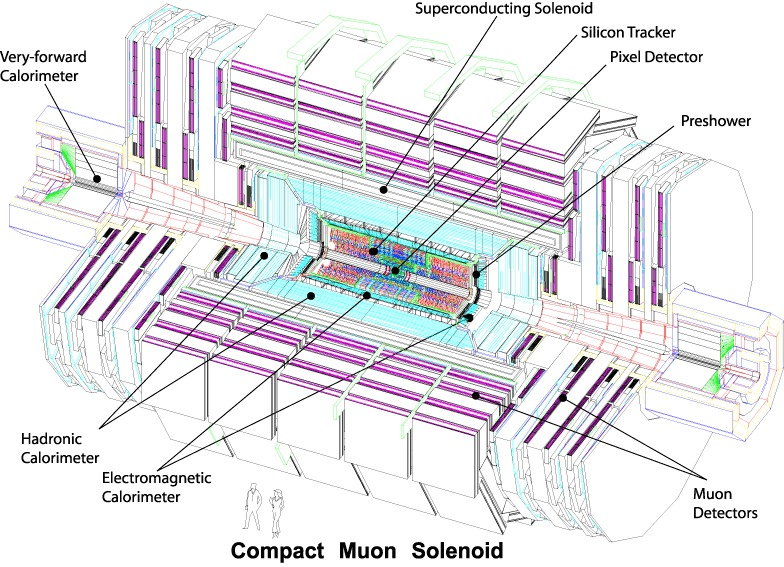
\includegraphics[width=.7\textwidth]{figures/cms_complete_layout.jpg}
\caption{An exploded view of the CMS detector.}
\label{figs:CMSLayout}
\end{figure}


\begin{figure}
\centering
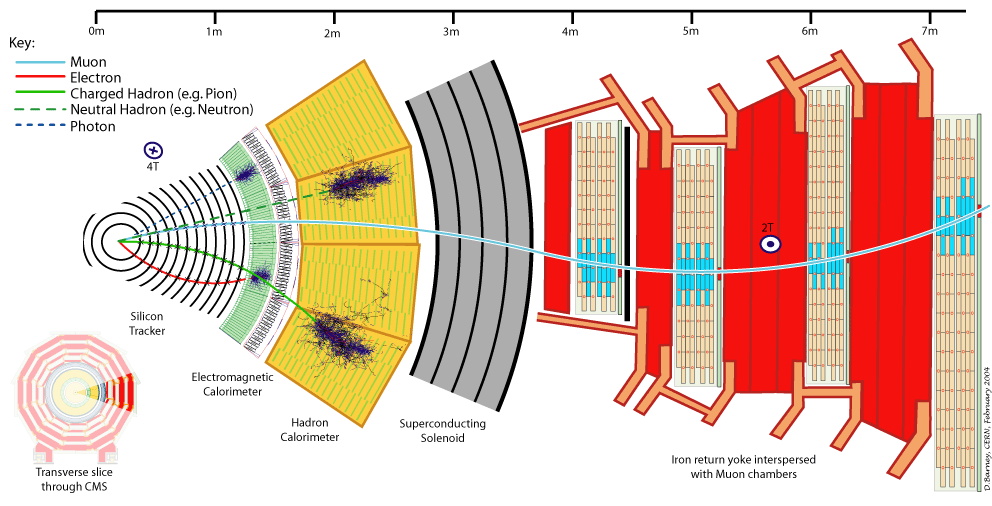
\includegraphics[width=.9\textwidth]{figures/CMS_Slice.png}
\caption{Transverse picture of the CMS detector. {\color{red} Change the picture to pdf format}}
\label{figs:CMS_Slice}
\end{figure}

\section{The beam: luminosity and cross-section}


\section{The coordinates}

\section{The Magnet}


In order to achieve good momentum resolution within a compact spectrometer without making stringent demands on muon-chamber resolution and alignment, a high magnetic field was chosen. The detailed parameters of this are shown in Table~\ref{table:magnet}.   The bore of the magnet coil is also large enough to accommodate the inner tracker and the calorimetry inside. 

\begin{table}[htb]
\caption{Parameters of the CMS superconducting solenoid.}
\begin{center}
\begin{tabular}{ |cc| }
\hline
Field           &  4 T \\
Inner Bore  &  5.9 m \\
Length        &  12.9 m \\
Number of turns &  2168 \\
Current   &        19.5 kA  \\
Store energy &  2.7 GJ \\
Hoop stress   &   64 atm \\
\hline
\end{tabular} 
\end{center}
\label{table:magnet}
\end{table}

\section{The inner tracking system}

{\color{red} Here we need a plot of the tracker layout and also the pixel tracker. If we could find a good description of the strip detector. }

The tracking volume is give by a cylinder of length 5.8 m and diameter 2.6 m.  In oder to deal with high track multiplicities, CMS employs 10 layers of silicon microstrip detectors, which provide the required granularity and precision.  In addition, 3 layers of silicon pixel detectors are placed closed to the interaction region to improve the measurement of impact parameter of charged-particle tracks, as well as the position of secondary vertices. 
The detailed layout of the tracker system is shown in Figure~\ref{fig:trackerLayout}

Close to the interaction vertex, in the barrel region, are 3 layers hybrid pixel detectors at a radii of 4.4, 7.3 and 10.2 cm.  
Each layer is spilt into segments like tiny kitchen tiles, each a little silicon sensor, 100 $\mu m$ by 
150 $\mu m$, about two hairs widths. Knowing which pixels have been touched allows us to deduce the particle$'$s trajectory. And because the detector is made of 2D tiles, rather than strips, and has a number of layers, we can create a three-dimensional picture.
The spatial resolution is measured to be $\approx$ 10 $\mu m$ for the $r-\phi$ measurement and $\approx$ 20 $\mu m$ for the $z$ measurement. 
After the pixels and on their way out of the tracker, particles pass through ten layers of silicon strip detectors, reaching out to a radius of 130 cm. The tracker silicon strip detector consists of four inner barrel (TIB) layers assembled in shells with two inner endcaps (TID), each composed of three small discs. The outer barrel (TOB) consists of six concentric layers. Finally two endcaps (TEC) close off the tracker. Each has silicon modules designed differently for its place within the detector.

\begin{figure}
\centering
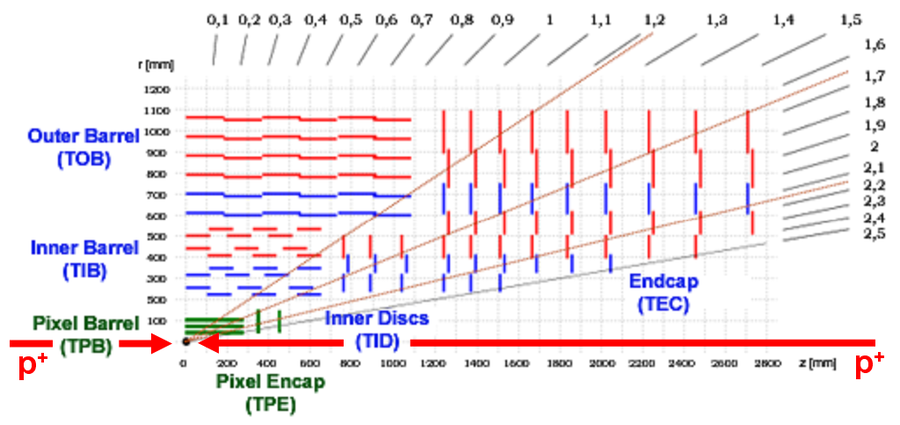
\includegraphics[width=1.4\textwidth]{figures/TrackerLayout.png}
\caption{The tracker layout of CMS}
\label{fig:trackerLayout}
\end{figure}

%In the barrel part, the silicon
%microstrip detectors are placed at $r$ between 20 and 110 cm.  The forward region has 2 pixel and 9 microstrip layers in each of the 2 endcaps.  The barrel part is separated into an Inner and an Outer Barrel.
%In order to avoid excessively shallow track crossing angles, the Inner Barrel is shorter than the Outer Barrel. 

% By considering the charged particle flux at various radii at high luminosity (Table~\ref{table:flux}), 3 regions can be delineated :
 
 %\begin{itemize}
 
 %\item  Closest to the interaction vertex where the particle flux is the highest ( $\approx 10^7 / s at r \approx 10 cm$), pixel detectors are placed, with an occupancy of about $10^{-4}$ per pixel per LHC crossing.  
 
 %\item In the intermediate region ( $20 < r < 55 cm$),  silicon microstrip detectors are used, leading to 
 %an occupancy of $\approx 2-3\% $/ LHC crossing. 
 
 %\item  In the outermost region ($r > 55 cm$) of the inner tracker, strip 
 
 %\end{itemize}  

\section{Electromagnetic calorimeter (ECAL) }

The ECAL is designed to calibrate the energy of electron and photons resulting from pp collisions, and its structure is shown in Figure~\ref{fig:ECAL} 
ECAL uses lead tungstate ($PbWO_4$) crystals with coverage in $|\eta|$ up to 3.0. 
This crystal is highly transparent and ``scintillates'' when electrons and photons pass through it, which  produces light in proportion to the particle$�$s energy. Although lead tungstate has short radiation (0.89 cm) and Moliere (2.2 cm) lengths, are also fast and radiation hard, it produces relatively low light yield. So the silicon avalanche photodiodes (APDs) are used as photodetectors in the ECAL barrel (EB) and 
 vacuum phototriodes (VPTs) in the ECAL endcap (EE). 
 
 
 \begin{figure}
\centering
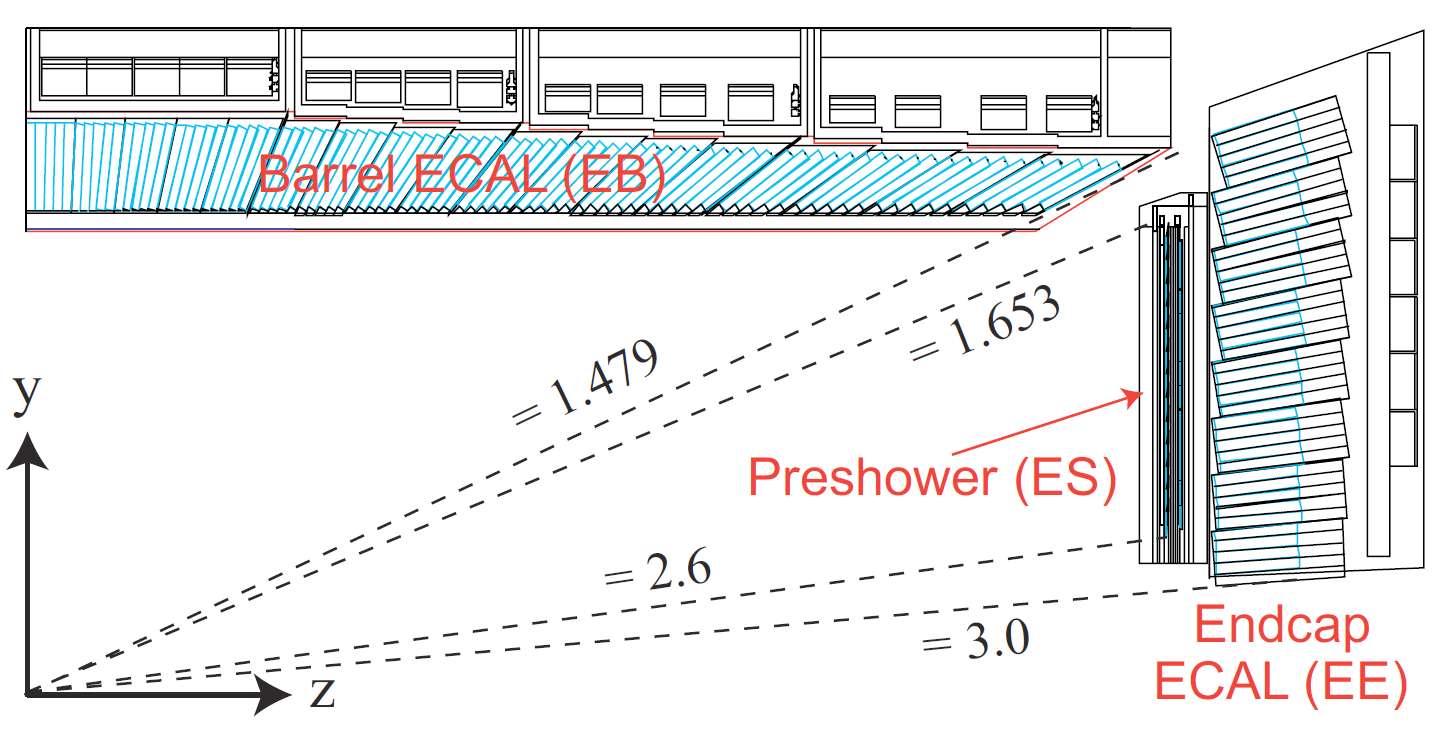
\includegraphics[width=.8\textwidth]{figures/ECALEta.png}
\caption{Geometric view of one quarter of the ECAL.}
\label{figs:ECAL}
\end{figure}

  
 These photodetectors that have been especially designed to work within the high magnetic field, are also glued onto the back of each of the crystals to detect the scintillation light and convert it to an electrical signal that is amplified and sent for analysis.
 
 A preshower system is installed in the front of EE.  
 The preshower is made of two planes of lead followed by silicon sensors, similar to those used in the tracker.  The reason for the preshower system is that short-lived particles called neutral pions, also produced in collisions, can inadvertently mimic high-energy photons when they decay into two closely-spaced lower energy photons that the ECAL picks up together. And for Higgs discovery,
 the high energy photons from Higgs decay is the important signature of $H \to \gamma \gamma$ channel. 
  

  \section{Hadronic calorimeter (HCAL)}
  
%  ECAL is surrounded by a brass/scintillator sampling hadron calorimeter with coverage up to $|\eta| < 3.0$. 



HCAL is designed to measure the energy of particles other than electron and photons, for example proton, neutron, pion and kaon.  It is also provide good containment and hermitically for the transverse missing energy $E_{T}^miss$ measurement, resulting from neutrinos or possible new particles. 

As shown in Figure~\ref{figs:HCAL},  HCAL is composed by four parts, HCAL barrel (HB), HCAL endocap (HE), HCAL outer (HO) and HCAL forward(HF).  HF is not presented in the plot. However, HF sits on the outside of the magnet and covers $3 <  |\eta| < 5.0$.  

HCAL is a brass/scintillator sampling hadron calorimeter. 
%{\bf HB}
 

\begin{figure}
\centering
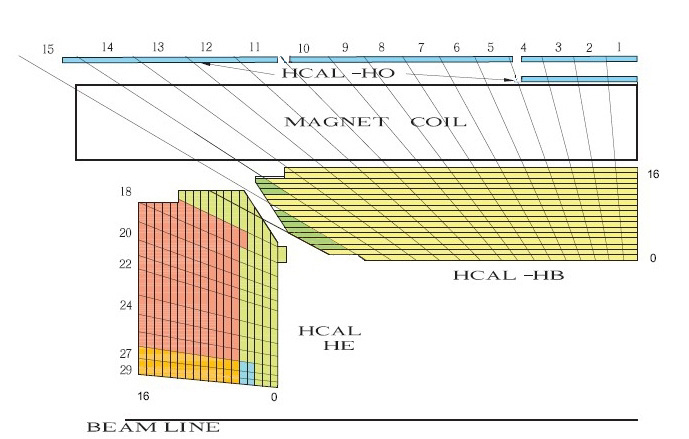
\includegraphics[width=.8\textwidth]{figures/Hcal.jpg}
\caption{Geometric view of one quarter of the HCAL. {\color{red} find a plot has HF}}
\label{figs:HCAL}
\end{figure}
  
  
\section{Muon system}
CMS is called the "compact muon solenoid". Muon detecting at CMS is very important. 
  
%Muons have a mass of 105.7 $MeV/c^2$, which is about 200 times that of the electron. Due to their greater mass, muons are not as sharply accelerated when they encounter electromagnetic fields, and do not emit as much bremsstrahlung (deceleration radiation). This allows muons of a given energy to penetrate far more deeply into matter than electrons, since the deceleration of electrons and muons is primarily due to energy loss by the bremsstrahlung mechanism. So muons could easily penetrate the ECAL. 
 
%Unlike hadron in HCAL, muon$'$s mass is much smaller than hadrons. Muon could 

Centrally produced muons are measured 3 times: in the inner tracker, after the coil , and in the return flux. Measurement of the momentum of muons using only the muon system is essentially determined by the muon bending angle at eh exit of the 4 T coil, taking the interaction point of pp collision as the origin of the muon.  For low-momentum muons, the best momentum resolution is given by the resolution 
obtained in the silicon tracker.  For high-momentum muons, combining the inner tracker and muon detector measurements will highly improve the muon momentum resolution.  
At CMS, in $0 < |\eta| < 2.0 $, for $\mu$ with $\pt$ $200 ~ 400$ GeV ,  $\delta p / p$ is measured to be $\leq 3\%$.


The layout of the one quarter of the CMS muon system for the initial low luminosity running is shown in 
Figure~\ref{fig:Muonsystem} and the transverse view of the muon stations (MS) are shown in 
Figure~\ref{fig:MuonStation}.  In the Muon Barrel (MB) region, 4 stations of detectors are arranged in cylinders interleaved with the iron yoke.  

Three types of gaseous detectors are used to identify and measure muons.{\color{red}cite some paper}. 
Drift tube (DT) is used in the barrel region ( $|\eta| < 1.2$).  In this region, the residual magnetic field in the chambers is low and also muon rate is low, so drift tube works well.  The maximum drift length is 2.0 cm and the single point resolution is $\approx$ 200 $\mu m$. 
In the endcap region,  cathode strip chambers (CSC) are used because of the high residual magnetic field and also high muon rate.  In addition to this,  resistive plate chambers (RPC) are used in both the barrel and the endcap regions. RPC could provide a fast response with good time resolution but with a coarser position resolutions than DTs and CSCs.  So RPC could identify the correct bunch crossing. 

\section{Trigger and data acuisistion}

%At LHC, protons collides 40 million times per second . 









\begin{figure}
\centering
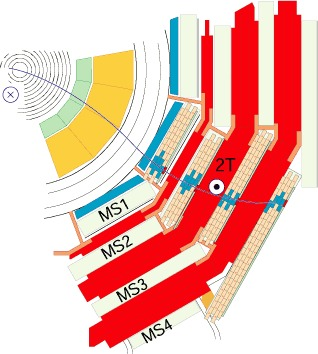
\includegraphics[width=.8\textwidth]{figures/MuStations.jpg}
\caption{The Muon stations in the transverse view}
\label{figs:MuonStation}
\end{figure}
  




\begin{figure}
\centering
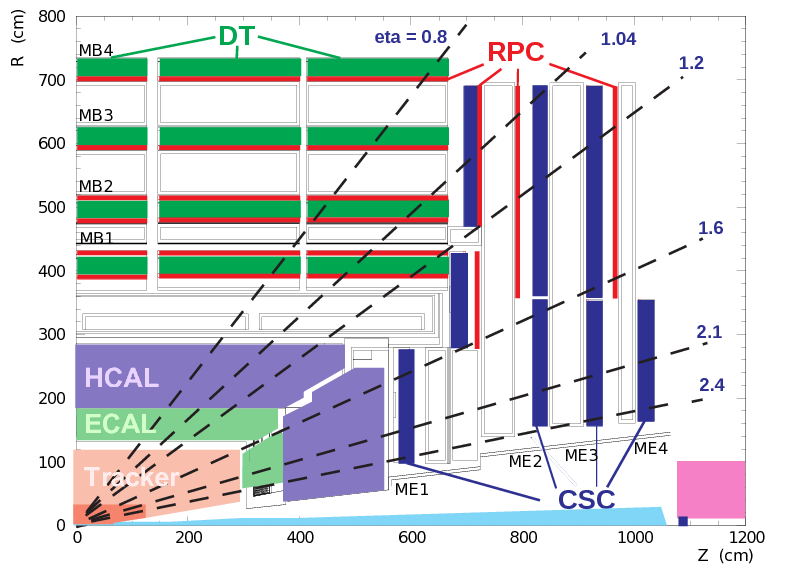
\includegraphics[width=.8\textwidth]{figures/Muonsystem.png}
\caption{Layout of one quarter of the CMS muon system for initial low luminosity running. The 
RPC system is limited to $|\eta| < 1.6$ in the endcap, and for the CSC system only the inner ring of the ME4 chambers  have been deployed. {\color{red} reference the book or the website}}
\label{figs:Muonsystem}
\end{figure}
  


\begin{figure}
\centering
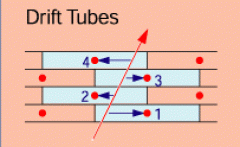
\includegraphics[width=.8\textwidth]{figures/DT.png}
\caption{Layout of the drift tube. }
\label{figs:DT}
\end{figure}

  



 
 
 







\chapter{Search for X $\to$ WH or ZH at LHC at $\sqrt{s} = 8$~TeV }
\label{chap:chapter4}
\section{Introduction}
\label{sec:introduction}


Several theories of physics beyond the standard model (SM) predict the
existence of vector resonances with
masses above 1\TeVcc that decay into
a W or Z vector boson (V)
 and a SM-like Higgs boson (H).
Here we present a search for 
the production of such resonances
 in proton-proton (pp) collisions at a
centre-of-mass energy of $\sqrt{s}=8$\TeVcc.  The data sample,
corresponding to an integrated luminosity of 19.7\fbinv, was collected
with the CMS detector at the CERN LHC.


%The following models of ${\rm \PWpr\to HW}$ and ${\rm Z'\to HZ}$ resonances are considered in this analysis.

The composite Higgs~\cite{Composite0,Composite1,Composite2} and little Higgs models~\cite{Han:2003wu}
address the issue of the hierarchy problem and predict many new particles,
%provide a direct solution to the hierarchy problem and 
including additional gauge bosons, e.g. heavy spin-1 $\PWpr$ or ${\rm Z'}$ bosons.
These models can be generalized in the Heavy Vector Triplet (HVT)~\cite{Pappadopulo:2014qza}
framework.
Of particular interest for this search is the HVT scenario B model, where
the branching fraction $\mathcal{B}({\rm W' \to WH})$ and $\mathcal{B}({\rm Z' \to ZH}) $ dominate over the corresponding 
branching fractions to fermions, and are comparable to $\mathcal{B}({\rm W' \to WZ})$ 
and $\mathcal{B}({\rm Z' \to WW})$. 
In this scenario, experimental constraints from searches for boson decay 
channels are more stringent than those from fermion decay channels. 
Several searches~\cite{Khachatryan:2014xja,
Aad:2014pha,Aad:2014xka,ATLASWWPAPER,EXO-12-024} 
for ${\rm W^\prime \rightarrow WZ}$ 
based upon the Extended Gauge Boson (EGB) reference 
model~\cite{egm} have excluded resonance 
masses below 1.7\TeVcc. Unlike the HVT scenario B model, 
the EGB model has enhanced fermionic couplings 
and the mass limit is not directly 
comparable to this work. Model independent limits on 
the cross section for the resonant 
production $\ell\nu+\mathrm{jets}$~\cite{EXO-13-009} can 
be used to extract resonance mass 
limits on the the processes ${\rm W^\prime\rightarrow WZ}$ 
and ${\rm Z^\prime \rightarrow WW}$ of 
1.7 TeV and 1.1 TeV, respectively.
A search for ${\rm Z^\prime \rightarrow ZH \rightarrow q\bar{q}}\tau\tau$
was reported in Ref.~\cite{cms-HZ-tautaujet} and
interpreted in the context of HVT scenario model B; however, 
no resonance mass limit could be set with the sensitivity achieved.
Finally, a recent search~\cite{Aad:2015yza} combining leptonic
decays of W and Z bosons, and two b-tagged jets forming a ${\rm \Hbb}$ candidate
excluded HVT model A with coupling constant $g_V = 1$ for heavy vector
boson masses below $m_{V'^0} < 1360~\GeV$ and $m_{V'^\pm} < 1470~\GeV$.

The signal of interest is a narrow heavy vector resonance ${\rm V'}$ decaying into
VH, where the V decays to a pair of quarks and the H decays either to
a pair of b quarks, or to a pair of W bosons, which further decay into
quarks.
The H in the HVT framework does not have properties that are identical 
to those of a SM Higgs boson. We make the assumption that the state 
observed by the LHC Collaborations~\cite{higgsdiscoveryAtlas,Chatrchyan:2012ufa} 
is the same as the one described by the HVT framework and 
that, in accord with present 
measurements~\cite{Khachatryan:2014kcaCMSHiggs1,Khachatryan:2014jbaCMSHiggs2,AtlasHiggs1}, 
its properties are similar to those of a SM Higgs boson.
  
In the decay of massive ${\rm V'}$ bosons 
produced in the pp collisions at the LHC, 
the momenta of the daughter V and H are large enough (${>} 200\GeV$) 
that their hadronic decay products 
are reconstructed as single jets~\cite{Gouzevitch:2013qca}. 
Because this results in a dijet topology, 
traditional analysis techniques relying on resolved jets are 
no longer applicable. The signal is characterized by a peak 
in the dijet invariant mass ($m_\mathrm{jj}$) distribution 
over a continuous background from mainly QCD multijet 
events. The sensitivity to b-quark jets 
from H decays is enhanced through 
subjet or jet b tagging~\cite{BTV-13-001}. 
Jets from ${\rm \Vqq}$, ${\rm \Hbb}$, and ${\rm \Hww}$ 
(virtual W denoted with an asterisk)
decays are identified with jet 
substructure techniques~\cite{topwtag_pas,JME-13-006}.


This is the first search for heavy resonances 
decaying via VH into all-jet final states 
and it incorporates the first application of jet substructure 
techniques to identify ${\rm \Hww}$ at a high Lorentz boost.


This analysis proceeds via the following steps:
\begin{enumerate}
\item The search is performed in the dijet sample, using the same
      preselection as the standard search for resonances decaying to 
      dijets~\cite{cmsdijet, cmsdijet8TeV}.

\item We identify events with one W/Z boson jet: a candidate
  jet originating from merged decaying products of W/Z:  
  \begin{itemize}
  \item we require a pruned jet mass cut, and
  \item an N-subjettiness cut preferring two-prong decays
  \end{itemize}
  (This is identical to Chapter~\ref{chap:chapter3}.)

\item We identify events with a highly boosted Higgs boson:
  \begin{itemize}
  \item we require a pruned jet mass cut, and
  \item two b tagged subjets, or 
  \item (when there are no two b tagged subjets) a N-subjettiness cut
    preferring four subjets
  \end{itemize}
  (The ${\rm \Hbb}$ tagging is synchronized with our sister analysis, the Radion
  search to the HH final state~\cite{HH4b}.)

\item After the full event selection, a potential signal would be
  characterized as a peak in the dijet invariant mass, on top of a
  falling background distribution.  

\item We model the background distribution with a smoothly falling 
  analytical function.  (The functional form is identical
  to the one used in Chapter~\ref{chap:chapter3}.)

\item We form the joint likelihood of several dijet distributions
  of V tagged and H tagged jets.  We include both two types of
  Higgs tags, and also low-purity Higgs and V taggers.  The background
  estimate procedure is the same in all channels -- analytical
  parametrization -- but is performed separately for each channel.

\item Finally, we set the limits on the various simplified models
  for resonances decaying to HV final states.

\end{enumerate}





%\section{Event reconstruction and selections}
\label{label:EventsReconstruction}

In proton-proton (pp) collisions at the energies reached at the LHC,  initials partons smashed to radiate quarks and gluons. As quarks and gluons have a net colour charge and cannot exist freely due to colour-confinement, they are not directly observed in Nature. 
Instead, they come together to form colour-neutral hadrons, a process called hadronisation that leads to a collimated spray of hadrons called a jet.



\section{Dijet analysis with jet substructure tagging}
\label{sec:analysis}

\section{Event display}
The event detected by the CMS detector is shown in Figure~\ref{fig:eventdisplay1}
and Figure~\ref{fig:eventdisplay2}. In Figure~\ref{fig:eventdisplay1}, the top image is
showing the event in the transverse plane, which is global $\theta-\phi$ axes. The bottom
image is showing this event in the $\theta-z$ plane. In Figure~\ref{fig:eventdisplay2}, the top 
image is showing the global view of this event. And the bottom image is showing
the lego plot of the two jets, each of which is composed by two subjets, a term that we will
introduce in the following text.  

\begin{figure}[!htbp]
\begin{center}
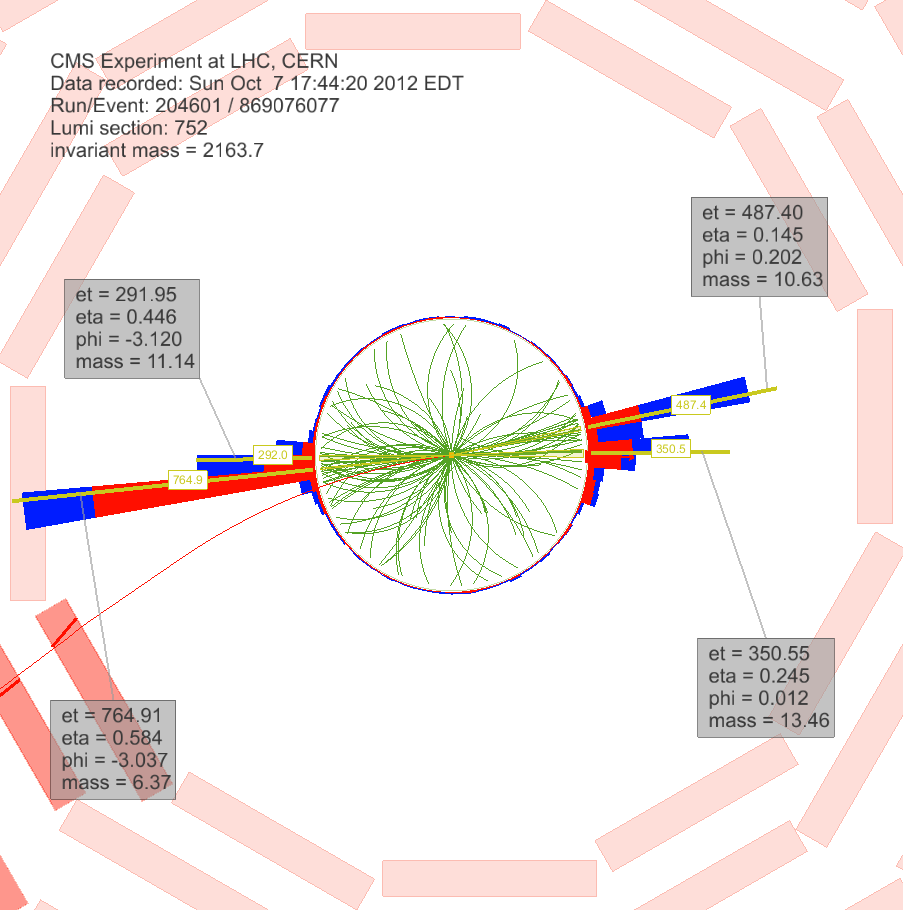
\includegraphics[width=0.6\textwidth,angle=0]{EXO-12-024/figs/event-display/highdoublemass/rho-phi-white.png}
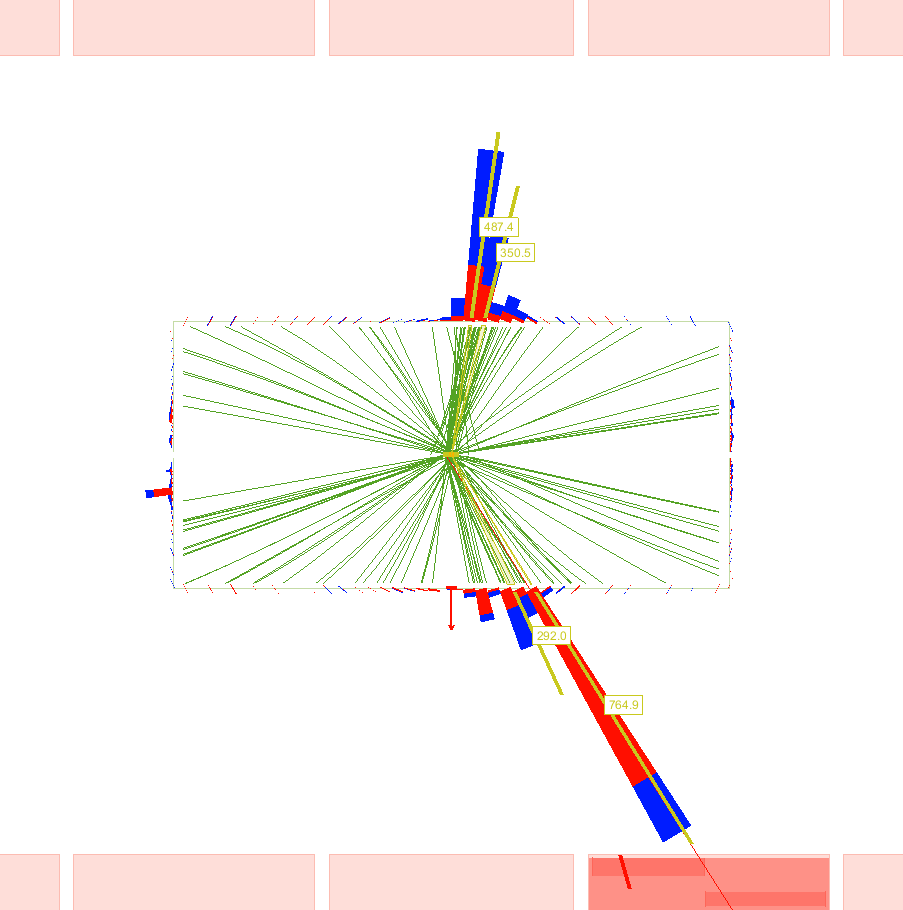
\includegraphics[width=0.6\textwidth,angle=0]{EXO-12-024/figs/event-display/highdoublemass/rho-z-white.png}
\end{center}
\caption{Event display of double W/Z-tagged event with the highest dijet invariant mass of 2.16~\TeVcc .
The transverse momenta of the two leading jets are 1.1~\TeVcc and 0.92~\TeVcc .
The invariant mass of the two leading pruned CA8 jets is 97.82 \GeVcc and 85.08 \GeVcc .
}
\label{fig:eventdisplay1}
\end{figure}

\begin{figure}[!htbp]
\begin{center}
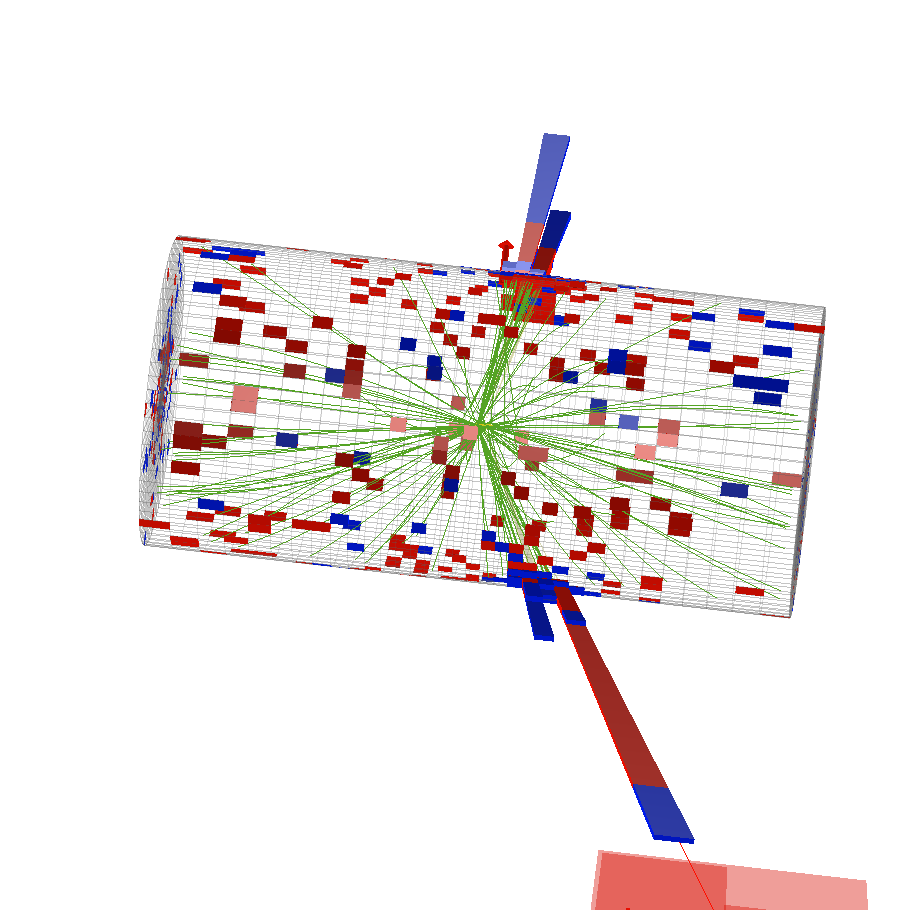
\includegraphics[width=0.6\textwidth,angle=0]{EXO-12-024/figs/event-display/highdoublemass/tower-white.png}
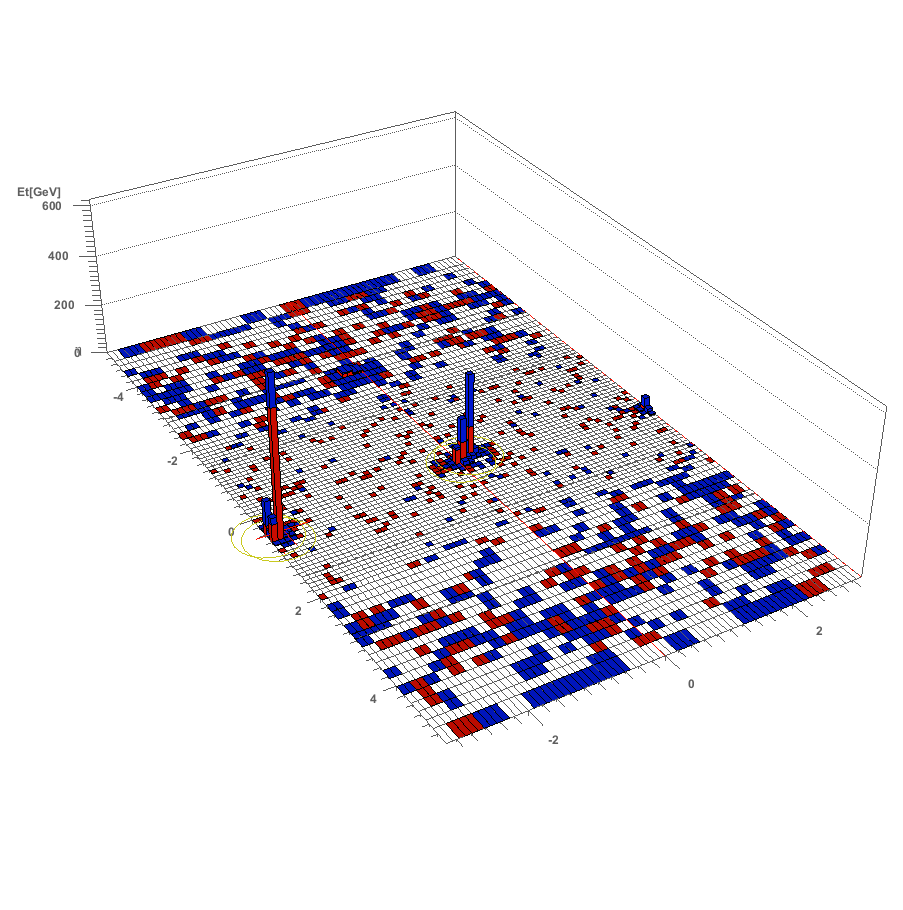
\includegraphics[width=0.6\textwidth,angle=0]{EXO-12-024/figs/event-display/highdoublemass/lego-white.png}
\end{center}
\caption{Event display of double W/Z-tagged event with the highest dijet invariant mass of 2.16~\TeVcc .
The transverse momenta of the two leading jets are 1.1~\TeVcc and 0.92~\TeVcc .
The invariant mass of the two leading pruned CA8 jets is 97.82 \GeVcc and 85.08 \GeVcc .
}
\label{fig:eventdisplay2}
\end{figure}


\subsection{Jet reconstruction}

\label{sec:reconstruction}


Based on CMSSW 5.3.x software package,events are reconstructed using the particle-flow reconstruction
algorithm~\cite{particleflow}, which attempts to reconstruct all
stable particles in an event by combining information from all
subdetectors. The algorithm categorizes all particles into five types:
muons, electrons, photons, charged and neutral hadrons. The resulting
particle flow candidates are passed to each jet clustering algorithm, in this case the
Cambridge-Aachen (CA)~\cite{CAaachen,CAcambridge}
jet clustering algorithm, as implemented in FastJet version 3.0.1 \cite{fastjet1,fastjet},
to create "particle flow jets".
The CA clustering sequence is only determined by the distance between
clusters and is not weighted by their momentum, as is done for the
$k_\text{T}$ and anti-$k_\text{T}$ algorithms. A distance parameter of
size $R=\sqrt{(\Delta \eta)^2 + (\Delta\phi)^2}=0.8$ is used for the CA algorithm.
%In previous studies based on simulation~\cite{catop_cms}, the CA algorithm was
%found to be more efficient (for the same mistag rate) than $k_{\mathrm  T}$
%or anti-$k_{\mathrm T}$ at finding hard subjets by reversing
%the last step of the clustering algorithm.


Charged hadrons identified as pileup are removed from the inputs to
the jet clustering algorithms.  The remaining neutral component of pileup
is removed by applying a residual area-based correction as
described in Ref.~\cite{jetarea_fastjet,jetarea_fastjet_pu}.  The mean
$\pt$ per unit area is computed with the $k_{\mathrm T}$ algorithm
with the ``active area'' method, with a distance parameter of 0.6, and
the jet energy is corrected by the amount of pileup expected in the
jet area. The amount of energy expected from the underlying event is
added back into the jet.  The pileup-subtracted jet four momenta are
finally corrected for nonlinearities in $\eta$ and $\pt$ with
simulated data, with a residual $\eta$-dependent correction added to
correct for the difference in simulated and true
responses~\cite{JME-JINST,Collaboration:2012dp}.

The jet energy corrections for the CA $R=0.8$ jets are derived from studies using the
anti-$k_{\mathrm T}$ $R=0.7$ jet algorithm. Simulation studies confirm that these
anti-$k_{\mathrm T}$-derived jet corrections
are adequate for the CA $R=0.8$ jet algorithm for the jet momenta
considered here~\cite{topwtag_pas}.% within an additional uncertainty of 2\%.


\subsection{Event selection}
\label{event_selection}

Events are selected using the following cuts:
\begin{itemize}
\item The event must have a well reconstructed primary vertex as computed by a deterministic annealing filter (DAF)
($\vert z_\text{Primary Vertex}\vert < 24$ cm, $N_\text{DOF} > 6$).
\item The following recommended noise event filters are used:
       \begin{itemize}
          \item  CSC tight beam halo filter
          \item  HBHE noise filter with isolated noise rejection
          \item  HCAL laser event filter (HBHE) and HCAL laser event filter 2012
          \item  ECAL dead cell trigger primitive (TP) filter
          \item  The beam scraping filter
          \item  Bad EE supercrystal filter
          \item  The tracking failure filter
          \item  Good primary vertex filter 
	  \item  Tracking coherent noise filter
	  \item  Tracking TOBTEC fakes filter  
       \end{itemize}
\item The events are required to have at least two ungroomed CA8 jets with
        \begin{itemize}
          \item $\pt > 30$ \GeVcc, $|\eta| < 2.5$
          \item  to have muon energy fraction $< 0.8$
          \item pass tight particle flow jet ID. The tight PF jet ID is listed below:
                 \begin{itemize}
                     \item   Neutral Hadron (EM) Fraction $< 0.90 (< 0.90)$, for all jet $\eta$
                     \item   Number of Constituents $> 1$, for all jet $\eta$
                     \item   Charged Hadron (EM) Fraction $> 0 (< 0.99)$, for jet $|\eta| < 2.4$
                     \item   Charged Multiplicity$ > 0$, for jet $|\eta| < 2.4$
                 \end{itemize}
        \end{itemize}
\item Beam background events are removed using the following requirements:
        \begin{itemize}
        \item In events with at least 10 tracks, a minimum of 25\% of
          these tracks must be high purity tracks.
        \end{itemize}
\item  We also require $E_{T}^{miss}/\sum{E_{T}} < 0.5$ to further suppress the noise producing large fake $E_{T}^{miss}$. 
\item The events must pass $|\Delta\eta|<1.3$, $m_{jj} > 890  \GeVcc$
\end{itemize}

This sample of dijet events is then tested for presence of
hadronically decaying W or Z bosons.
 
\newpage
\section{Data and Monte Carlo samples}
\label{sec:data_and_mc_samples}


The data sample of proton-proton collisions at $\sqrt{s}=8$~\TeVcc was collected in 2012 and corresponds to
an integrated luminosity of \intlumi.
The datasets and also the certifications
used are summarized in Table~\ref{table:dataset}. 
The dijet sample is dominated by light flavored and gluon jets, which we denote as 
the "QCD background".  The QCD background is obtained from data by fitting an
analytic parameterization of the dijet invariant mass distribution.

Signal events have been simulated using
{\sc jhugen}~\cite{Gao:2010qx,Bolognesi:2012mm},
\PYTHIA~6.426~\cite{pythia} and \HERWIG{++} 2.5.0~\cite{herwig} event
generators and processed through a simulation of the CMS detector,
based on \GEANTfour~\cite{refGEANT}.  \PYTHIA~6 is used with
CTEQ61L~\cite{cteq} and \HERWIG{++} with MRST2001~\cite{mrst} parton
distribution functions.  Tune Z2* (a modification of tune
Z1~\cite{bib_tunez1}) is used with \PYTHIA~6, while the tune version
23 is used with \HERWIG{++}.  The process $\cPq^* \to \PW/\cPZ +
\text{jet}$ is generated using \PYTHIA~6.  RS graviton production is
studied with $k/\MPl=0.1$, which determines a resonance width of about
1\% of the resonance mass which is about a factor five smaller than
the experimental resolution for dijets.  While \HERWIG{++} contains a
more detailed description of the angular distributions for \GRS than
\PYTHIA~6 for this process~\cite{resonanceshape} and is therefore used
to model the \GRS resonance shape, the \PYTHIA~6 cross section is used
to maintain consistency with reference models used in related
analyses~\cite{CMSZZPAS2}.  Bulk graviton production is studied with
$k/\MPl=0.2$ and is generated with {\sc jhugen} interfaced with
\PYTHIA~6 for the showering.
Bulk graviton cross sections are calculated using CalcHEP.
The process $\PWpr \to \PW\cPZ$ is generated using \PYTHIA~6 with Standard
Model $V-A$ couplings and without applying k-factors.  

To validate our RS graviton resonance Monte Carlo, we compare Pythia6, Herwig++ and 
a generator including full angular correlations developed by the JHU group (which
we denote ``JHU generator'').
Figure~\ref{fig:compare-Herwig++-Pythia6} shows the comparsions of invariant mass and
$\Delta\eta$ of two Z bosons at generator level, in which Herwig++ and
Pythia6 are compared with the JHU generator which describes the
angular distributions exactly.  Pythia6 does not implement the angular
correlations, and from Figure~\ref{fig:compare-Herwig++-Pythia6} one can indeed conclude
that in its description of this effect it is inferior to Herwig++.

\begin{figure}[htb]
\begin{center}
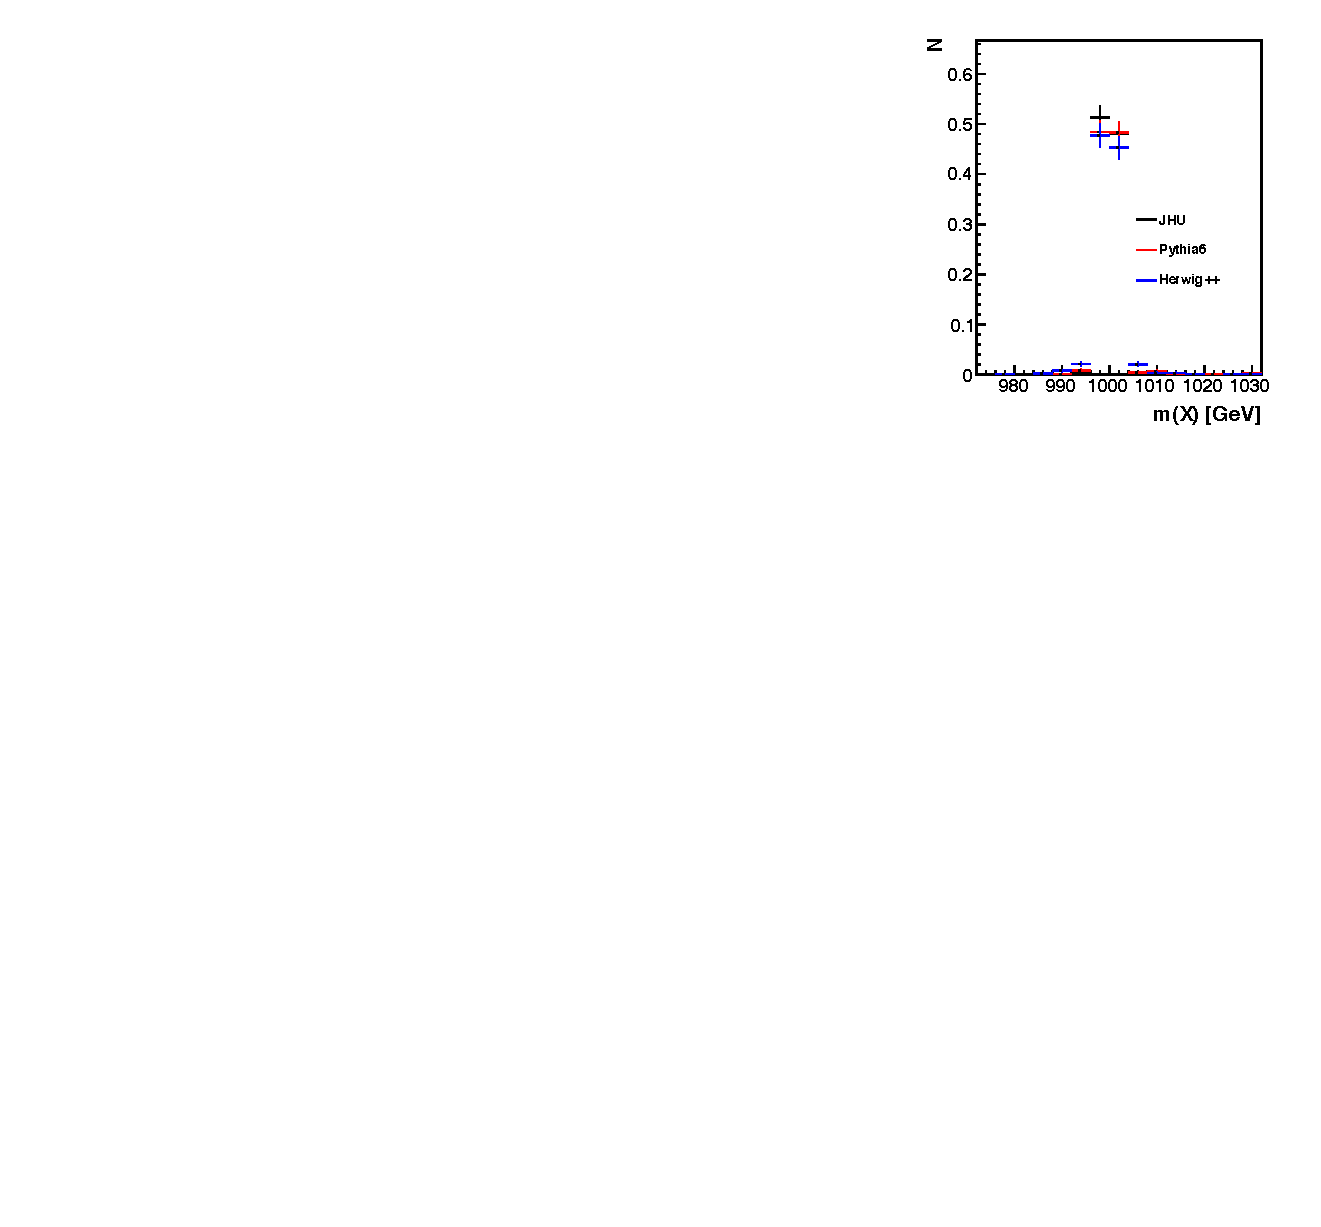
\includegraphics[width=0.43\textwidth]{EXO-12-024/figs/comparison-jhu-pythia-herwigg/MX.pdf}
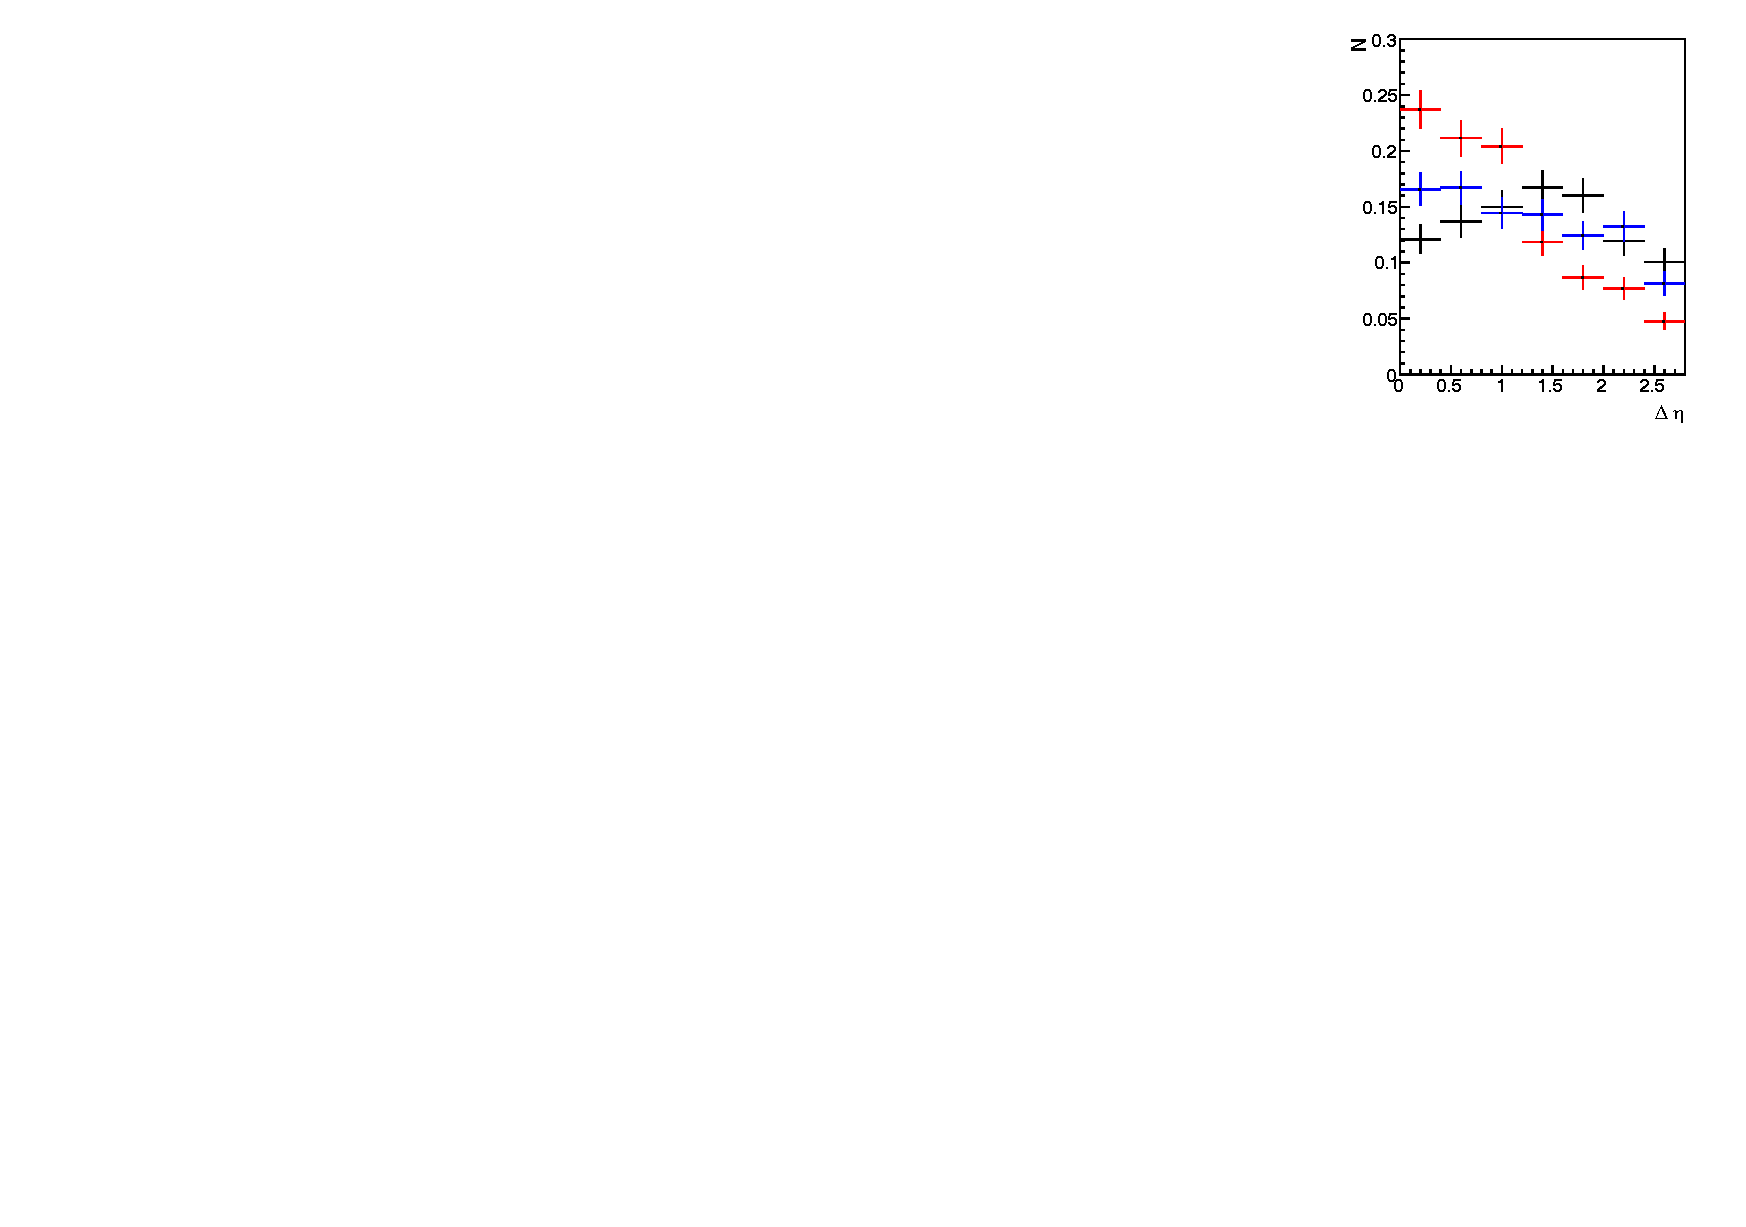
\includegraphics[width=0.43\textwidth]{EXO-12-024/figs/comparison-jhu-pythia-herwigg/delta-y.pdf}
\end{center}
\caption{Invariant mass and $\Delta\eta$ of two Z bosons at generator level for Pythia6 and Herwig++ models of a 1~\TeVcc RS graviton resonance with $k/M_{PL}=0.02$ with the JHU generator which includes all angular correlations.}
\label{fig:compare-Herwig++-Pythia6}
\end{figure}

All Monte Carlo events are fully simulated and reconstructed via the Geant4-based CMS simulation
 and reconstruction software.

Tables~\ref{table:singletag}, \ref{table:doubletag}, \ref{table:doubletagbulk} and \ref{table:doubletag2} summarize the new 
physics simulation datasets used in this analysis. 


\begin{table}[htb]
\begin{center}
\begin{tabular}{ |l| }
\hline
Dataset                                 \\
\hline
/Jet/Run2012A-22Jan2013-v1/AOD  \\
/JetHT/Run2012B-22Jan2013-v1/AOD  \\
/JetHT/Run2012C-22Jan2013-v1/AOD  \\
/JetHT/Run2012D-22Jan2013-v1/AOD  \\
\hline
\end{tabular} 
\end{center}
\caption{Summary of 8~\TeVcc collision data used in this analysis. 
The certification file used for these data is 
{\tt Cert\_190456-208686\_8TeV\_22Jan2013ReReco\_Collisions12\_JSON.txt
}.
}
\label{table:dataset}
\end{table}


\begin{table}[htb]
\begin{center}
\begin{tabular}{ |l|c|r|r| }
\hline
Process           & Generator& Events & X-sec[pb] \\
\hline
qW(m=750$\GeVcc$) &Pythia6   &30000   &1.133E+02  \\
qW(m=1000$\GeVcc$)&Pythia6   &30000   &2.647E+01  \\
qW(m=1500$\GeVcc$)&Pythia6   &30000   &2.540E+00  \\
qW(m=2000$\GeVcc$)&Pythia6   &30000   &3.510E-01  \\
qW(m=3000$\GeVcc$)&Pythia6   &30000   &1.008E-02  \\

qZ(m=750$\GeVcc$) &Pythia6   &30000   &4.071E+01  \\
qZ(m=1000$\GeVcc$)&Pythia6   &30000   &9.405E+00  \\
qZ(m=1500$\GeVcc$)&Pythia6   &30000   &8.937E-01  \\
qZ(m=2000$\GeVcc$)&Pythia6   &30000   &1.231E-01  \\
qZ(m=3000$\GeVcc$)&Pythia6   &30000   &3.465E-03  \\
\hline
\end{tabular}
\end{center}
\caption{Summary of the simulated Monte Carlo samples used in this analysis for process
 $q* \to Z/W + jet$}
\label{table:singletag}
\end{table}


\begin{table}[htb]
\begin{center}
\begin{tabular}{ |l|c|r|r| }
\hline
Process            & Generator             & Events& Pythia6 x-sec [pb] \\
\hline
WW(m=750$\GeVcc$)  &Herwig++/Pythia6 Z2*   &30000  & 2.220E+00\\
WW(m=1000$\GeVcc$) &Herwig++/Pythia6 Z2*   &30000  & 4.254E-01 \\
WW(m=1500$\GeVcc$) &Herwig++/Pythia6 Z2*   &30000  & 3.298E-02 \\
WW(m=2000$\GeVcc$) &Herwig++/Pythia6 Z2*   &30000  & 4.083E-03 \\
WW(m=2500$\GeVcc$) &Herwig++/Pythia6 Z2*   &30000  & 6.191E-03 \\
WW(m=3000$\GeVcc$) &Herwig++/Pythia6 Z2*   &30000  & 1.010E-04 \\
ZZ(m=750$\GeVcc$)  &Herwig++/Pythia6 Z2*   &30000  & 1.120E+00 \\
ZZ(m=1000$\GeVcc$) &Herwig++/Pythia6 Z2*   &30000  & 2.137E-01 \\
ZZ(m=1500$\GeVcc$) &Herwig++/Pythia6 Z2*   &30000  & 1.662E-02 \\
ZZ(m=2000$\GeVcc$) &Herwig++/Pythia6 Z2*   &30000  & 2.027E-03 \\
ZZ(m=2500$\GeVcc$) &Herwig++/Pythia6 Z2*   &30000  & 3.077E-04 \\
ZZ(m=3000$\GeVcc$) &Herwig++/Pythia6 Z2*   &30000  & 5.099E-05 \\
\hline
\end{tabular}
\end{center}
\caption{Summary of the simulated Monte Carlo samples used in this analysis for process
 $G_{RS} \to WW, ZZ$.}
\label{table:doubletag}
\end{table}

\begin{table}[htb]
\begin{center}
\begin{tabular}{ |l|c|r|r| }
\hline
Process           & Generator& Events & X-sec[pb] \\
\hline
WZ(m=750$\GeVcc$) &Pythia6   &30000   &5.391E-01  \\
WZ(m=1000$\GeVcc$)&Pythia6   &30000   &1.444E-01 \\
WZ(m=1500$\GeVcc$)&Pythia6   &30000   &1.804E-02  \\
WZ(m=2000$\GeVcc$)&Pythia6   &30000   &3.129E-03  \\
WZ(m=2500$\GeVcc$)&Pythia6   &30000   &6.781E-04  \\
WZ(m=3000$\GeVcc$)&Pythia6   &30000   &1.894E-04  \\
\hline
\end{tabular}
\end{center}
\caption{Summary of the simulated Monte Carlo samples used in this analysis for process
 $W' \to WZ$.}
\label{table:doubletag2}
\end{table}


\begin{table}[htb]
\begin{center}
\begin{tabular}{ |l|c|r|r| }
\hline
Process            & Generator             & Events & X-sec[pb] \\
\hline
WW(m=1000$\GeVcc$) &JHU Z2*   &50000  &0.001774 \\
WW(m=1500$\GeVcc$) &JHU Z2*   &50000  &9.207E-05 \\
WW(m=2000$\GeVcc$) &JHU Z2*   &50000  &8.004E-06 \\
WW(m=2500$\GeVcc$) &JHU Z2*   &50000  &8.851E-07 \\
WW(m=3000$\GeVcc$) &JHU Z2*   &50000  &- \\
ZZ(m=1000$\GeVcc$) &JHU Z2*   &50000  &0.0009044 \\
ZZ(m=1500$\GeVcc$) &JHU Z2*   &50000  &4.622E-05 \\
ZZ(m=2000$\GeVcc$) &JHU Z2*   &50000  &4.029E-06 \\
ZZ(m=2500$\GeVcc$) &JHU Z2*   &50000  &4.460E-07 \\
ZZ(m=3000$\GeVcc$) &JHU Z2*   &50000  &- \\
\hline
\end{tabular}
\end{center}
\caption{Summary of the simulated Monte Carlo samples used in this analysis for process
 $G_{Bulk} \to WW, ZZ$.}
\label{table:doubletagbulk}
\end{table}

Table~\ref{table:singletag} describes a single-tagged process: $q* \to W/Z + jet$
with a large cross section. We generated the MC using Pythia6 with Tune Z2*.
The configuration is in the appendix of this note.
The parameters \verb+RTCM(43)+, \verb+RTCM(44)+, \verb+RTCM(45)+ are set to 1 and the scale \verb+RTCM(41)+ is set to the resonance mass \verb+PMAS(343,1)+$=$\verb+PMAS(344,1)+. 
Only decays in to qW or qZ are allowed.
We generate the process $q* \to W/Z + jet$ using Pythia6 with Tune Z2*.

Table~\ref{table:doubletag} shows a double-tagged process: $G_{RS} \to WW/ZZ$.
This is produced using Herwig++ with Tune23 and as a cross check also in Pythia6 with Tune Z2*. 
In Pythia6, the parameter \verb+PARP(50)+ corresponding to $5.4 k/\bar{M}_{Pl}$ which impacts the width and 
cross section of the resonance.
In Herwig++, the cross section and width are given by the ratio of \verb+RS/Model:Lambda_pi+ and the resonance mass  \verb+/Herwig/Particles/Graviton:NominalMass+.
The process $G_{RS} \to WW/ZZ$ is generated using Herwig++ with Tune23 and its cross section is taken from Pythia6 with Tune Z2*.
We study RS graviton production with $k/\bar{M}_{Pl}=0.1$, defining a resonance width smaller than the experimental resolution for dijets.
Table~\ref{table:doubletag2} describes another double-tagged process:
$W' \to WZ$. This is produced using Pythia6 with Tune Z2*.
The decay of the $W'$ is restricted to $WZ$ with \verb+MDME(331,1)=1+.
The process $W' \to WZ$ is generated using Pythia6 with Tune Z2*.
All Monte Carlo events are fully simulated
and reconstructed via the CMS
simulation and reconstruction software. 

\newpage

\section{Trigger}
\label{sec:trigger}


Events are selected if one of the following triggers has fired: HLT\_HT750, HLT\_PFHT650, HLT\_PFNoPUHT650,
HLT\_FatDiPFJetMass750\_DR1p1\_Deta1p5.  All versions of each of these triggers are used. None of these triggers are prescaled druing the 2012 data taking period. HLT\_PFNoPUHT650 trigger is used for the data set after the RunC(including RunC), while HLT\_PFHT650
trigger is only used for RunA and RunB data sets. 


Figure~\ref{fig:trigger efficiencies part1}, Figure~\ref{fig:trigger efficiencies part2}, and Figure~\ref{fig:trigger efficiencies part3} show the trigger efficiencies of the OR of the highest threshold HLT\_PFHT650 trigger and the HLT\_FatJetMass trigger w.r.t. an OR of the lower threshold HLT\_HT550 trigger. From the plot, the trigger is $99\%$ effiecient above 890\GeVcc for the untagged, single tagged and double tagged data. 


\begin{figure}[htb]
\centering
     \resizebox{0.75\linewidth}{!}{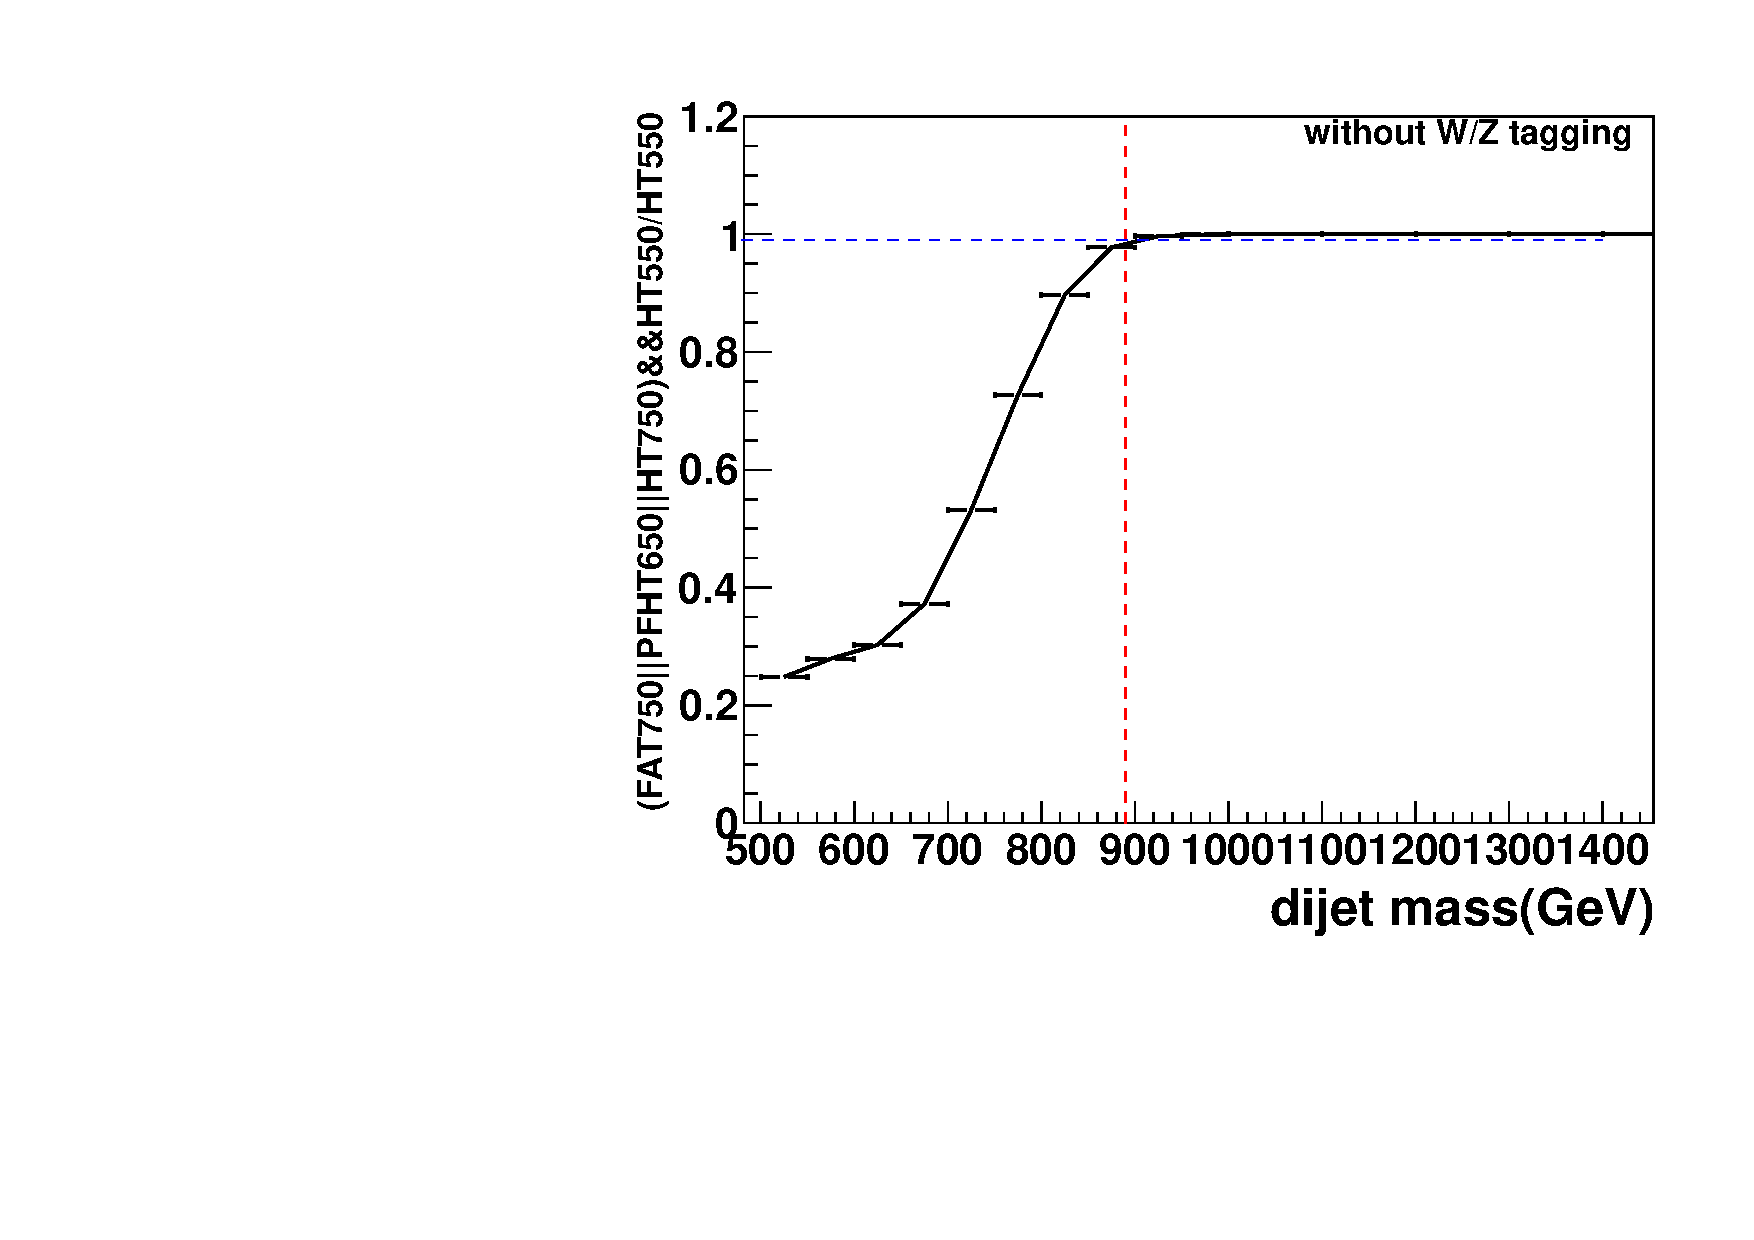
\includegraphics{EXO-12-024/figs/trigger-eff/Dataeff_withouttagging.pdf}} \\   
\caption[Trigger efficiencies]{Trigger efficiency for untagged data of FAT\_750$\parallel$HLT\_PF(NoPU)HT650$\parallel$HLT\_HT750 measured using data collected by lower threshold $H_T550$ trigger. The dash red line is positioned at $m_{jj}$ equal $890 GeV$, the blue line is at efficiency at 99$\%$. }
  \label{fig:trigger efficiencies part1}
\end{figure}

\begin{figure}[htb]
\centering
     \resizebox{0.75\linewidth}{!}{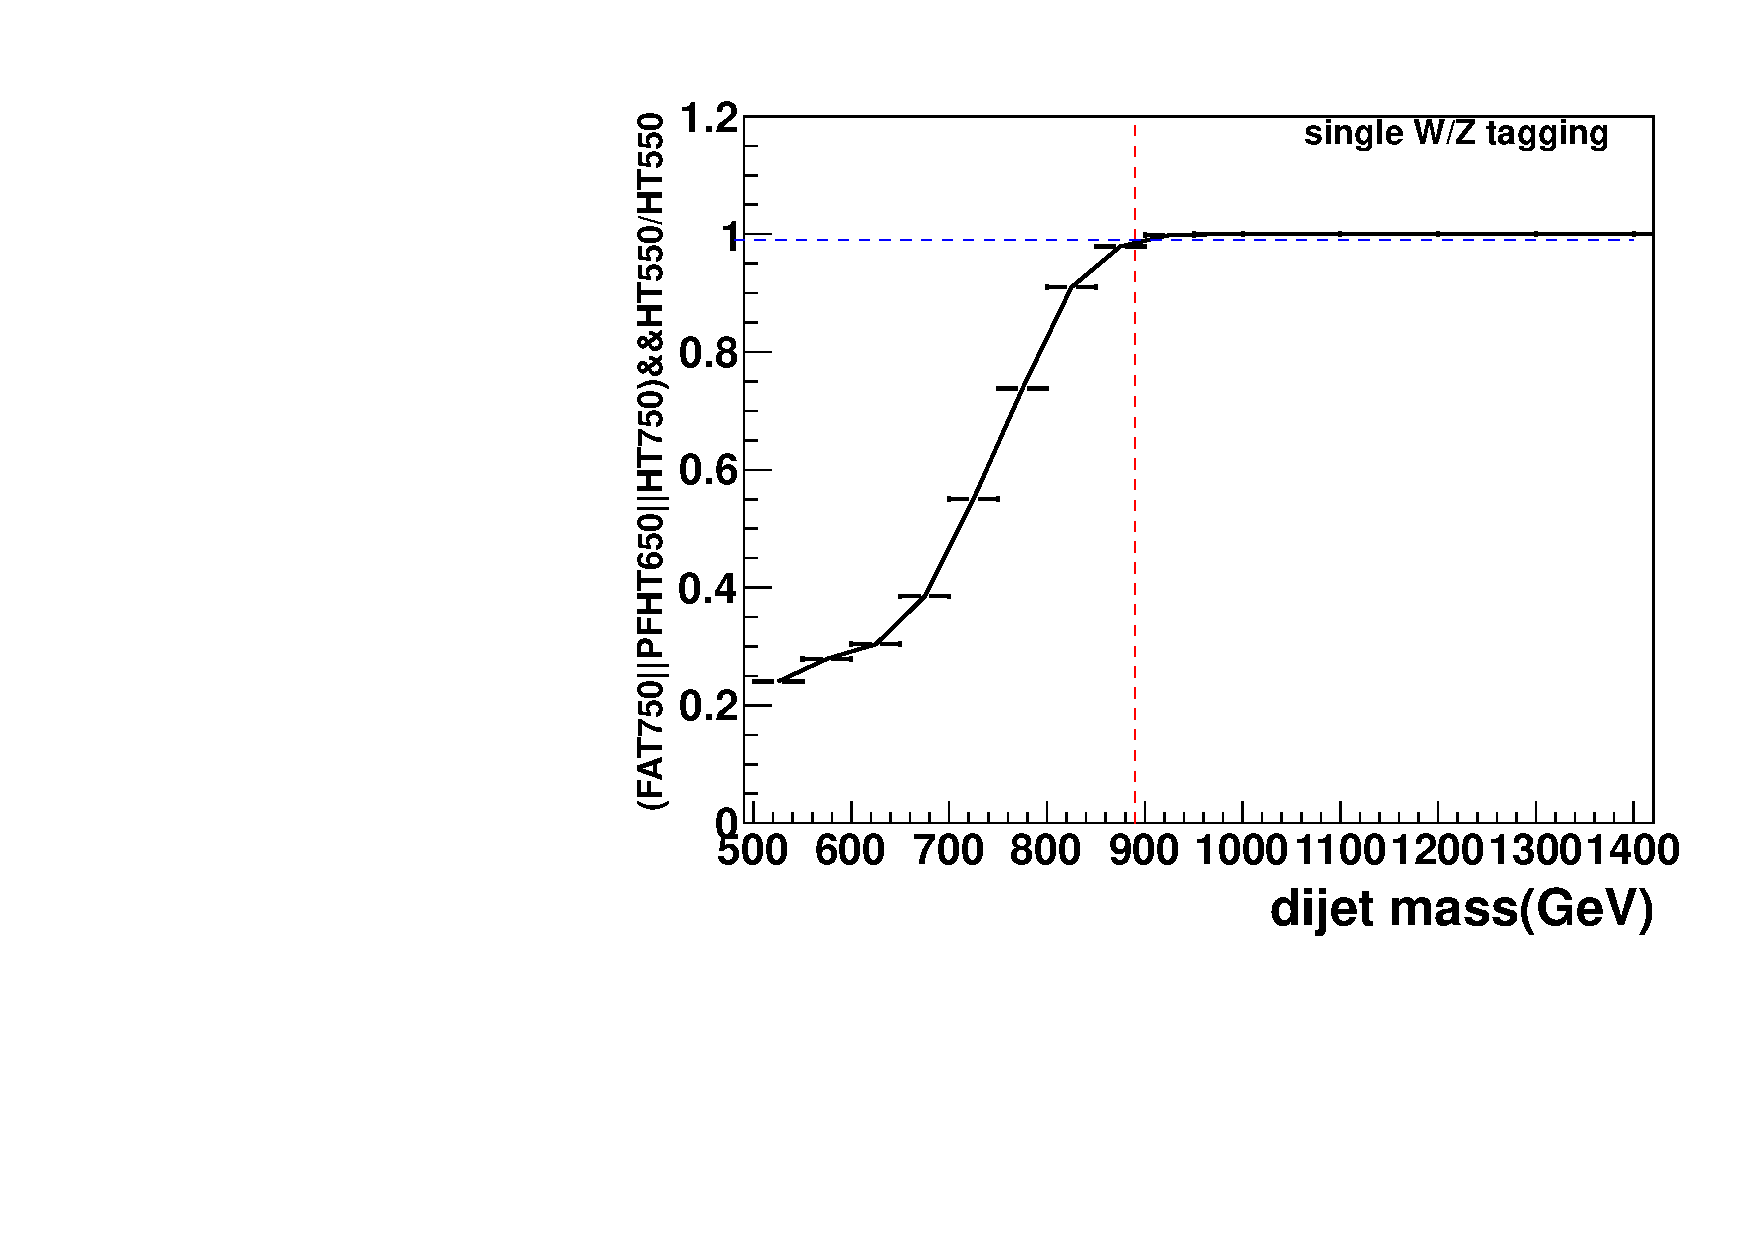
\includegraphics{EXO-12-024/figs/trigger-eff/Dataeff_singletagging.pdf}}  \\
\caption[Trigger efficiencies]{Trigger efficiency for single tagged data of FAT\_750$\parallel$HLT\_PF(NoPU)HT650$\parallel$HLT\_HT750 measured using data collected by lower threshold $H_T550$ trigger. The dash red line is positioned at $m_{jj}$ equal $890 GeV$, the blue line is at efficiency at 99$\%$. }
  \label{fig:trigger efficiencies part2}
\end{figure}

\begin{figure}[htb]
\centering
     \resizebox{0.75\linewidth}{!}{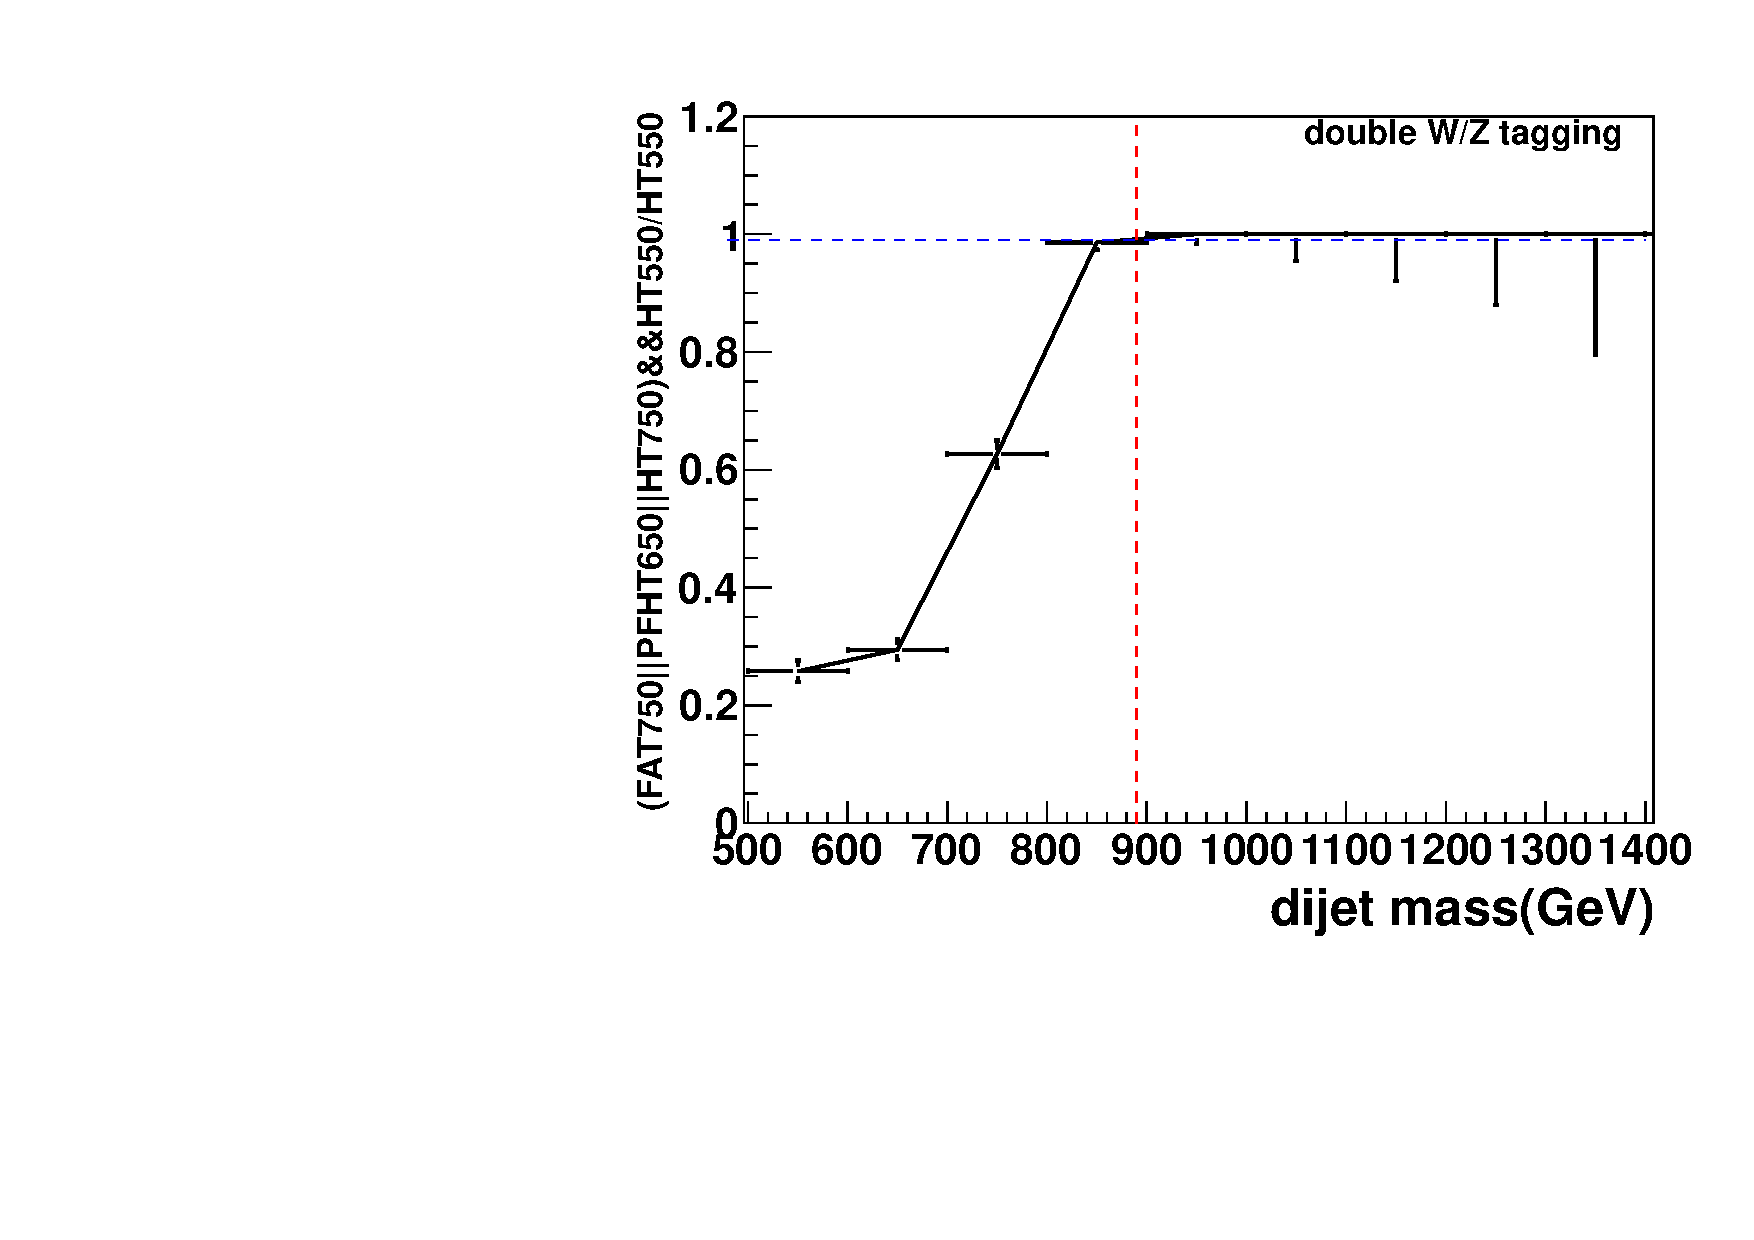
\includegraphics{EXO-12-024/figs/trigger-eff/Dataeff_doubletagging.pdf}} \\
\caption[Trigger efficiencies]{Trigger efficiency for double tagged data of FAT\_750$\parallel$HLT\_PF(NoPU)HT650$\parallel$HLT\_HT750 measured using data collected by lower threshold $H_T550$ trigger. The dash red line is positioned at $m_{jj}$ equal $890 GeV$, the blue line is at efficiency at 99$\%$. }
  \label{fig:trigger efficiencies part3}
\end{figure}


\clearpage














\newpage
\section{Data and MC comparisons}
\label{sec:data-mc-comp}

In this section, we compare some kinematic features of the jets between QCD MC and data, which are
 shown in Fig~\ref{fig:mjjSingle}, \ref{fig:mjjDouble},\ref{fig:dySingle}, \ref{fig:dyDouble}, \ref{fig:dphiSingle}, 
\ref{fig:dphiDouble},\ref{fig:metSumPtSingle},
\ref{fig:Pt0Single}, \ref{fig:Pt0Double}, \ref{fig:Pt1Single}, \ref{fig:Pt1Double},
\ref{fig:Eta0Single}, \ref{fig:Eta0Double}, \ref{fig:Eta1Single}, \ref{fig:Eta1Double},
%\ref{fig:CA8Single},\ref{fig:CA8Double}
and \ref{fig:massNsub}.
Predictions from Pythia6 with Tune $Z2*$ and Herwig++ with Tune 23 are shown.
The comparison is shown in the exclusive dijet category, low and high purity,  single and double tagged events..
The distributions are shown after the event selection (in particular $|y| < 2.5$, $|\Delta\eta|<1.3$, $m_{jj} > 890  \GeVcc$) is applied.
The number of data events in each mass bin are shown in Table~\ref{table:eventnumbers}.
The MC is normalized to the number of data events in each category and the shapes are compared.


\begin{table}[htb]
%\begin{center}
\begin{tabular}{|p{3.0cm}|p{3.0cm}|p{3.0cm}|p{3.0cm}|p{3.0cm}|}
%\begin{tabular}{|c|c|c|c|c|}
\hline
lower mass bin border & low purity 1-tag events & high purity 1-tag events& low purity 2-tag events& high purity 2-tag events\\
\hline
890 & 165671 & 105892 & 7586 & 2544 \\ 
944 & 115622 & 72007 & 4950 & 1673 \\ 
1000 & 80537 & 48930 & 3311 & 1005 \\ 
1058 & 56423 & 33398 & 2159 & 658 \\ 
1118 & 39817 & 23086 & 1407 & 427 \\ 
1181 & 27651 & 15817 & 962 & 302 \\ 
1246 & 19531 & 10741 & 647 & 175 \\ 
1313 & 13617 & 7477 & 434 & 135 \\ 
1383 & 9880 & 5128 & 272 & 75 \\ 
1455 & 6992 & 3578 & 195 & 49 \\ 
1530 & 4939 & 2525 & 138 & 25 \\ 
1607 & 3443 & 1658 & 86 & 24 \\ 
1687 & 2454 & 1160 & 52 & 10 \\ 
1770 & 1744 & 815 & 42 & 9 \\ 
1856 & 1193 & 547 & 35 & 6 \\ 
1945 & 881 & 389 & 21 & 4 \\ 
2037 & 643 & 230 & 12 & 3 \\ 
2132 & 402 & 167 & 8 & 3 \\ 
2231 & 287 & 99 & 5 & 1 \\ 
2332 & 193 & 86 & 3 &  \\ 
2438 & 138 & 57 & 1 &  \\ 
2546 & 87 & 28 & 0 &  \\ 
2659 & 60 & 13 & 2 &  \\ 
2775 & 48 & 11 &  &  \\ 
2895 & 38 & 5 &  &  \\ 
3019 & 14 & 4 &  &  \\ 
3147 & 17 & 3 &  &  \\ 
3279 & 4 & 1 &  &  \\ 
3416 & 4 & 0 &  &  \\ 
3558 & 4 & 1 &  &  \\ 
3704 &  & 1 &  &  \\ 
3854 &  &  &  &  \\ 
4010 &  &  &  &  \\ 
\hline
\end{tabular}
\caption{Number of events in each mass bin exclusive, with 1 W/Z-tag and  2 W/Z-tags required in low
purity and high purity categories.}
\label{table:eventnumbers}
\end{table}



\newpage


\begin{figure}[htb]
\centering
\begin{tabular}{cc}
     \resizebox{0.5\linewidth}{!}{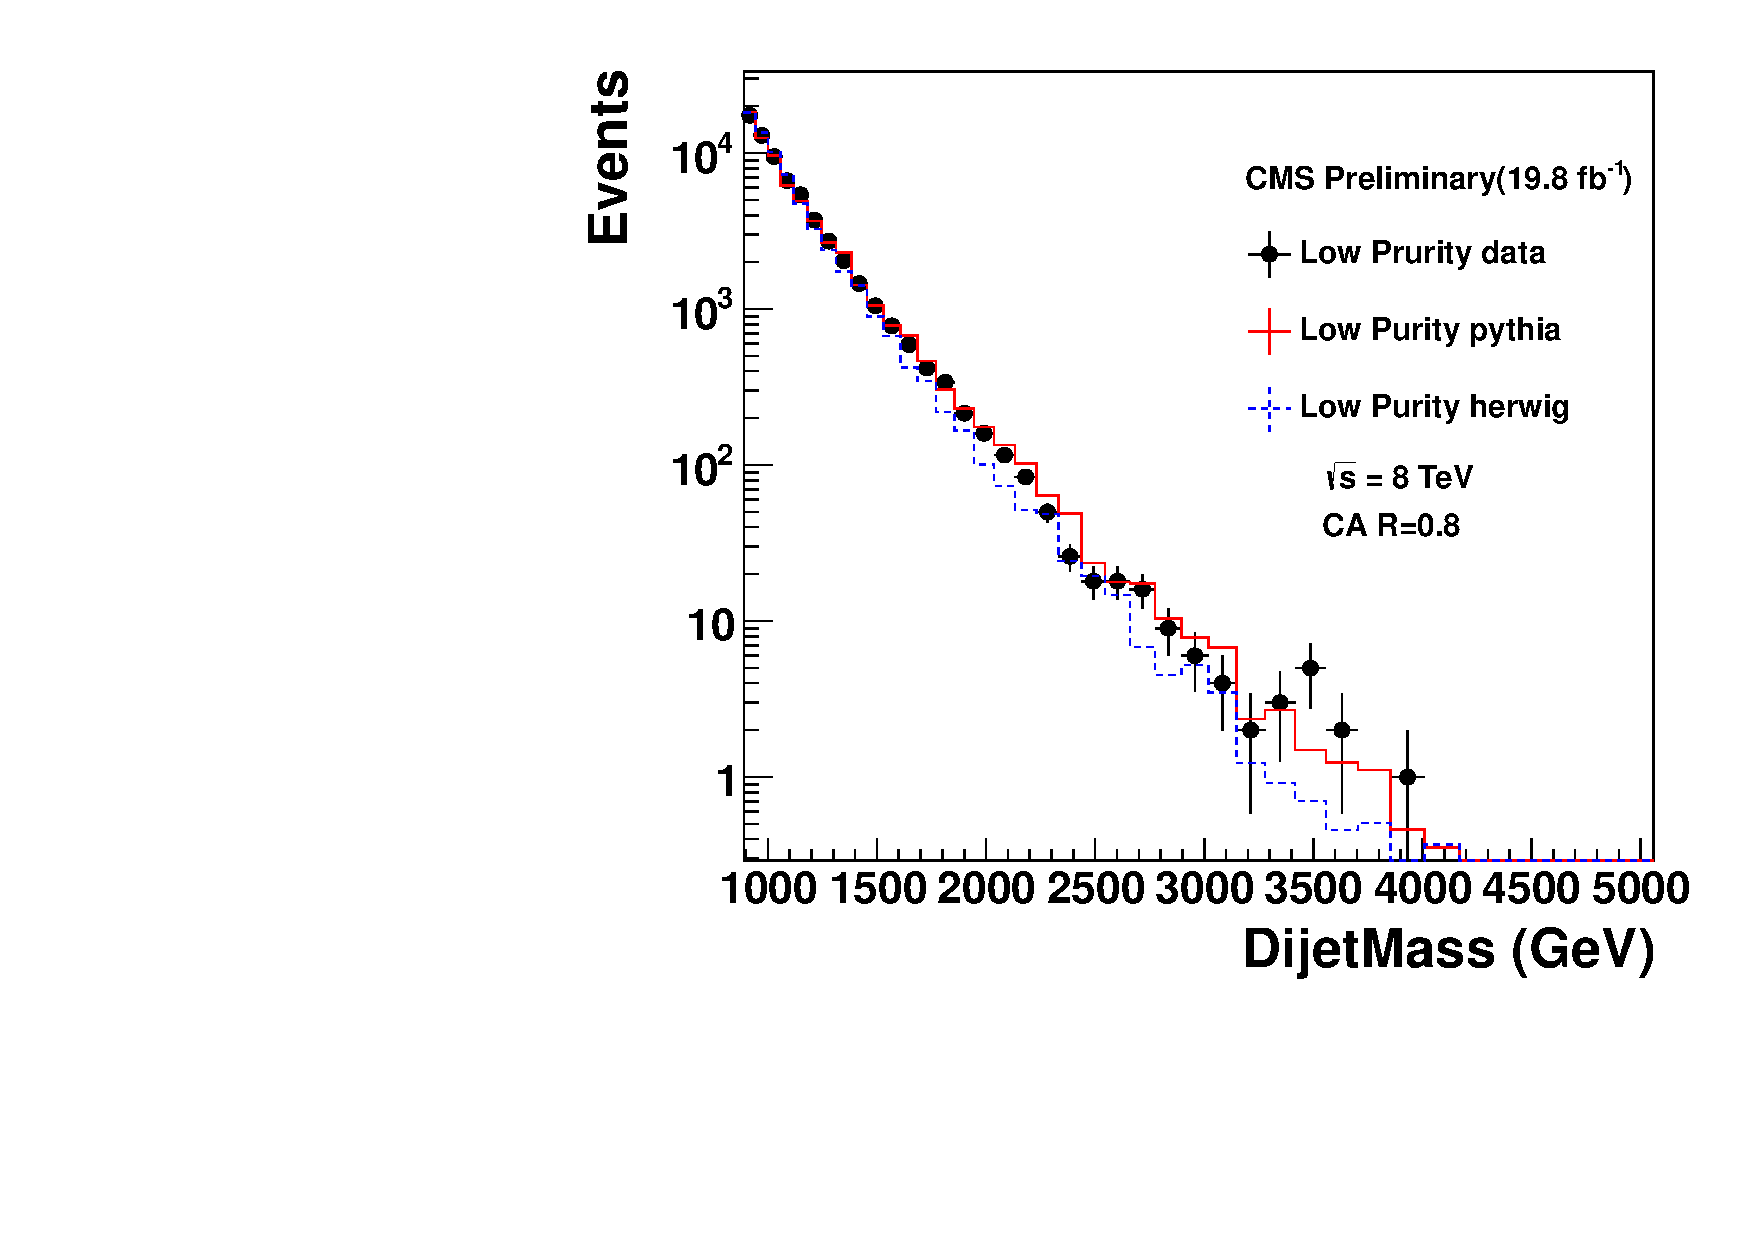
\includegraphics{figs/Data-MC-comparisons/DijetMass-qVLowP.pdf}} &
     \resizebox{0.5\linewidth}{!}{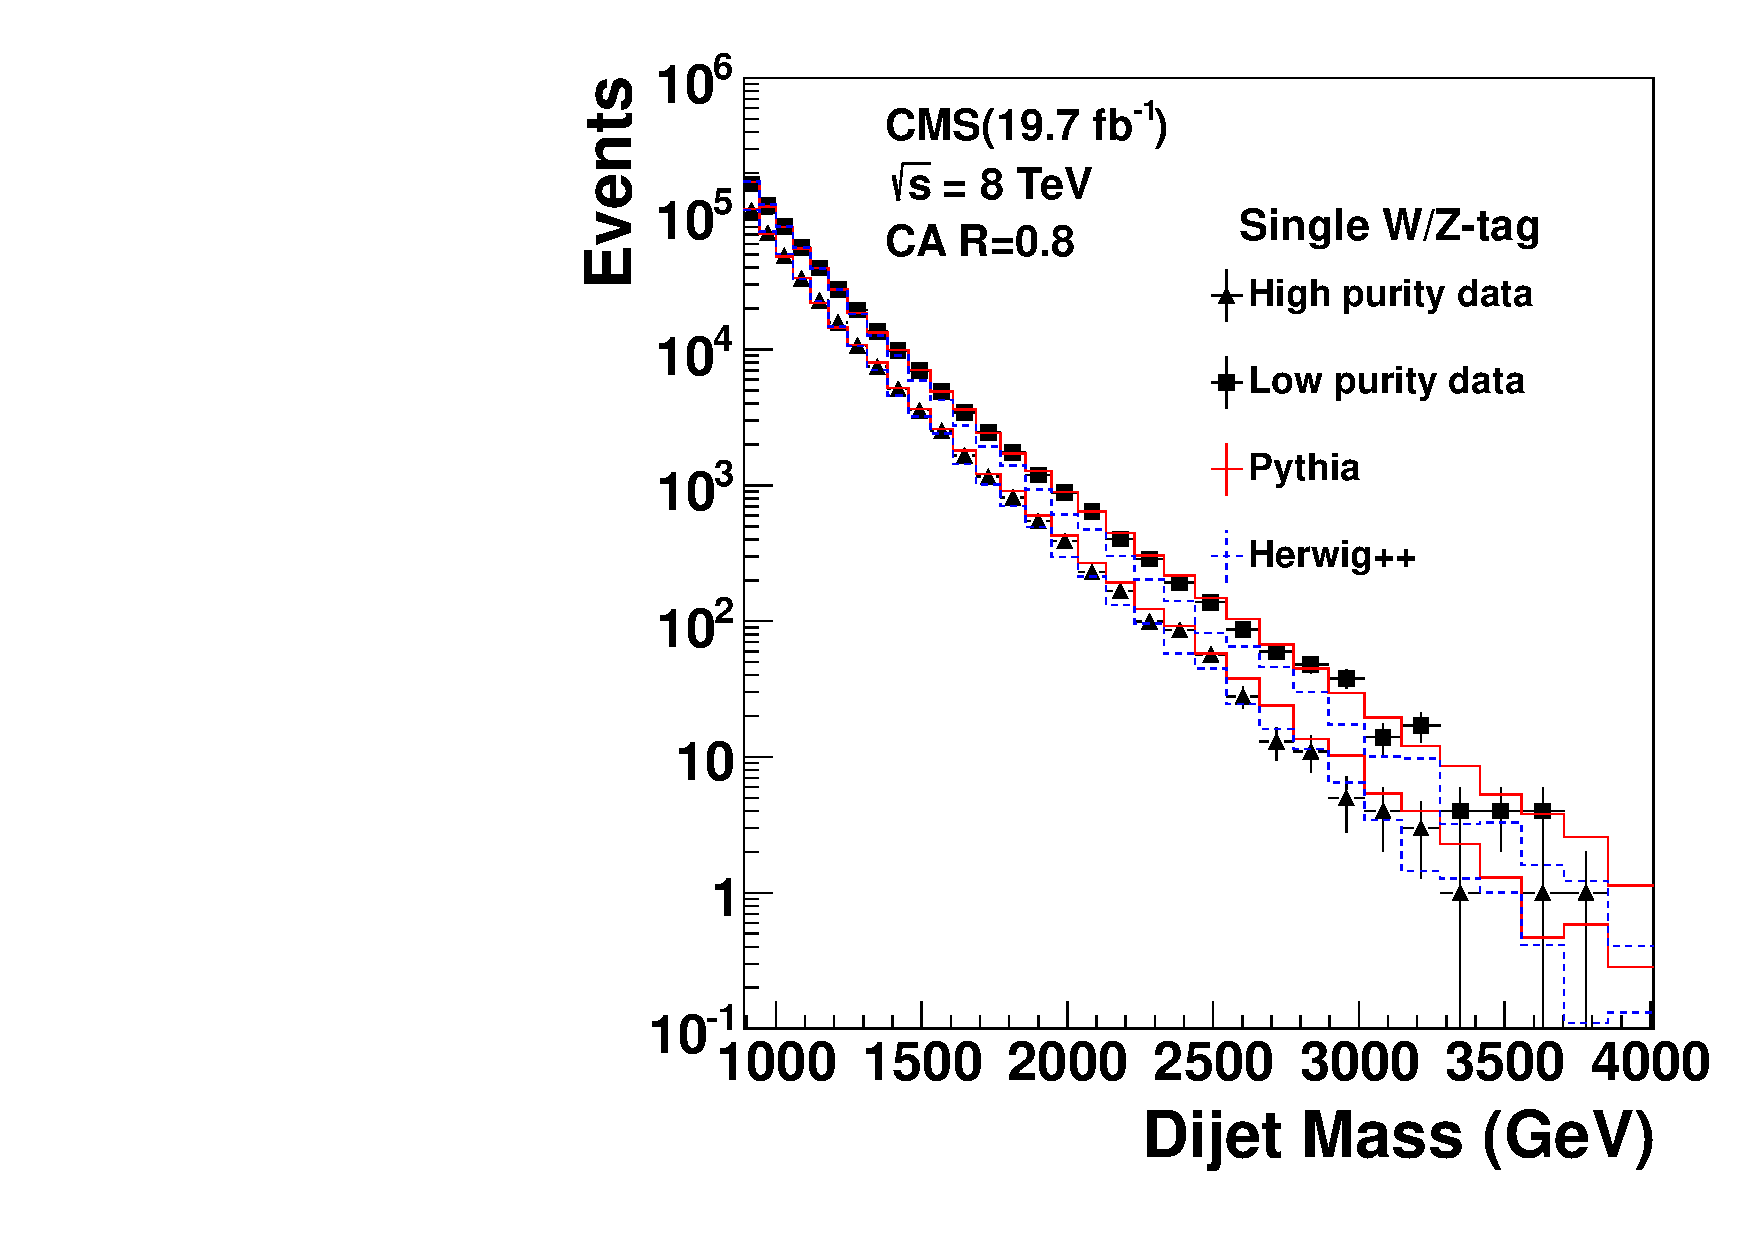
\includegraphics{figs/Data-MC-comparisons/DijetMass-qVMiumHigh.pdf}} \\
\end{tabular}
  \caption[Invariant Mass Single]{Comparisons between data and Monte Carlo
           for invariant mass of the two leading jets of low purity (left) and low-high purity (right) 1-tagged events.
           The MC is normalized to the number of data events in each category.
           }
  \label{fig:mjjSingle}
\end{figure}

\begin{figure}[htb]
\centering
\begin{tabular}{cc}
     \resizebox{0.5\linewidth}{!}{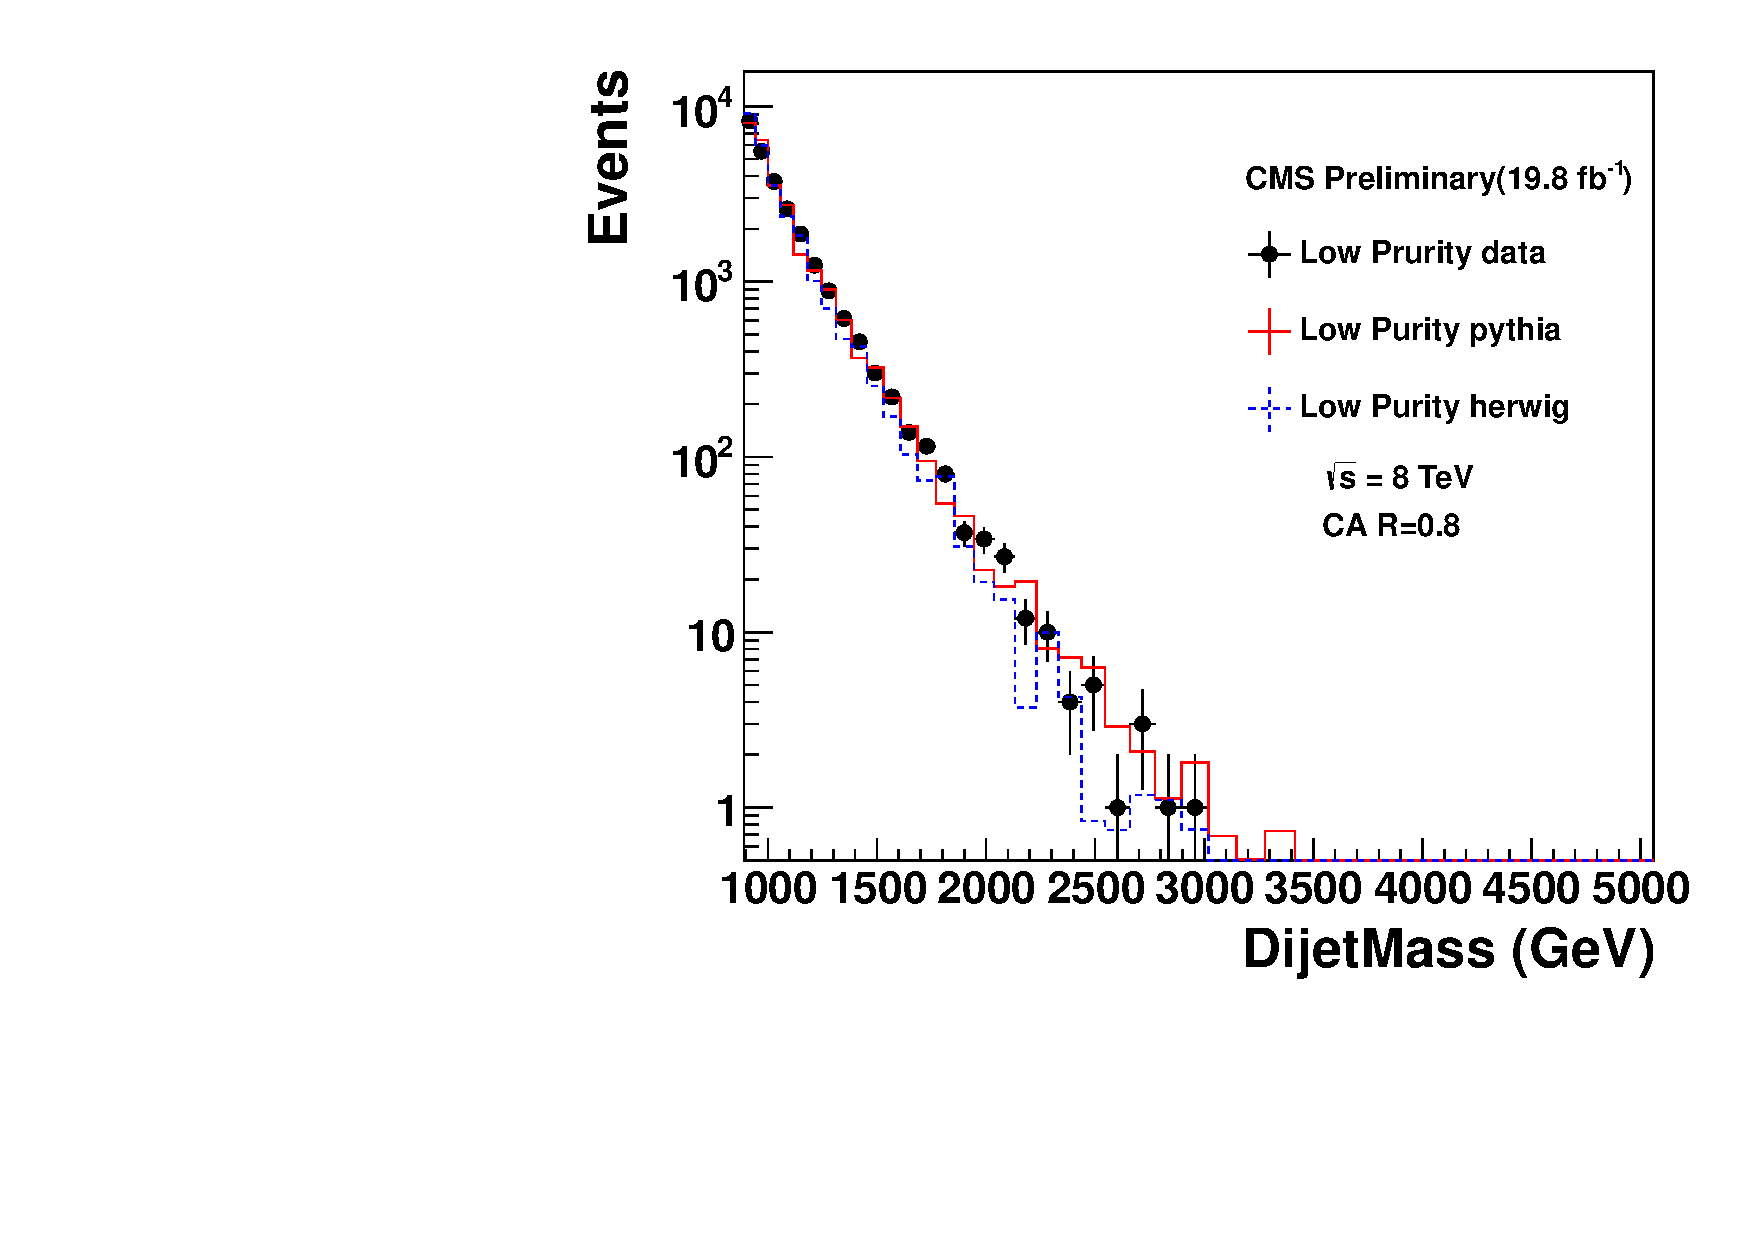
\includegraphics{figs/Data-MC-comparisons/DijetMass-VVLowP.pdf}} &
     \resizebox{0.5\linewidth}{!}{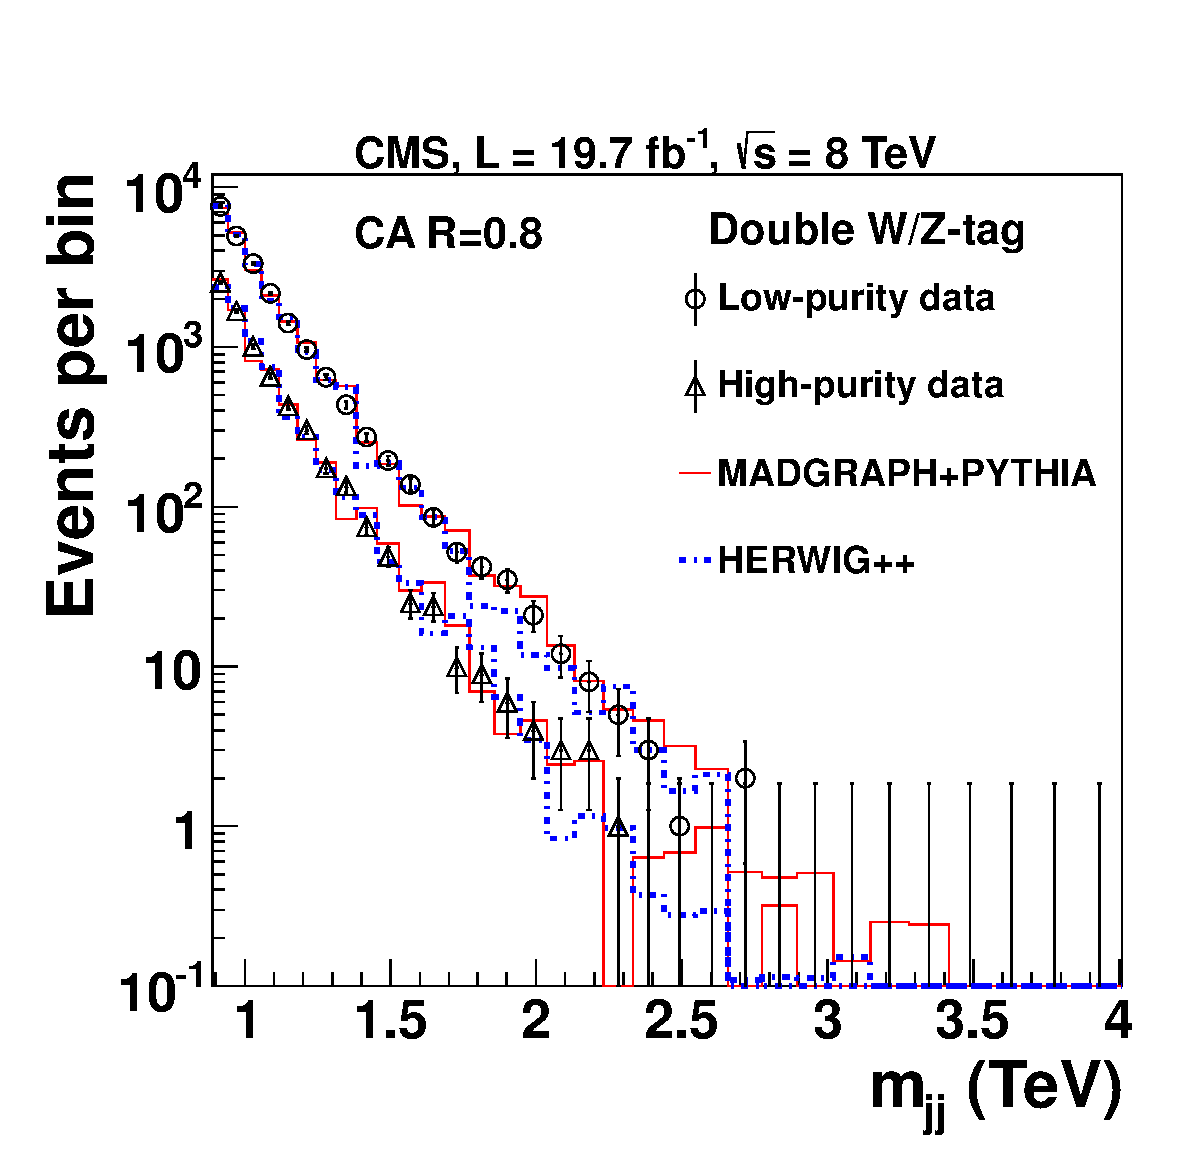
\includegraphics{figs/Data-MC-comparisons/DijetMass-VVMiumHigh.pdf}} \\
\end{tabular}
  \caption[Invariant Mass Double]{Comparisons between data and Monte Carlo
           for invariant mass of the two leading jets of low purity (left) and low-high purity (right) 2-tagged events.
           The MC is normalized to the number of data events in each category.
           }
  \label{fig:mjjDouble}
\end{figure}

\newpage
\begin{figure}[htb]
\centering
\begin{tabular}{cc}
     \resizebox{0.5\linewidth}{!}{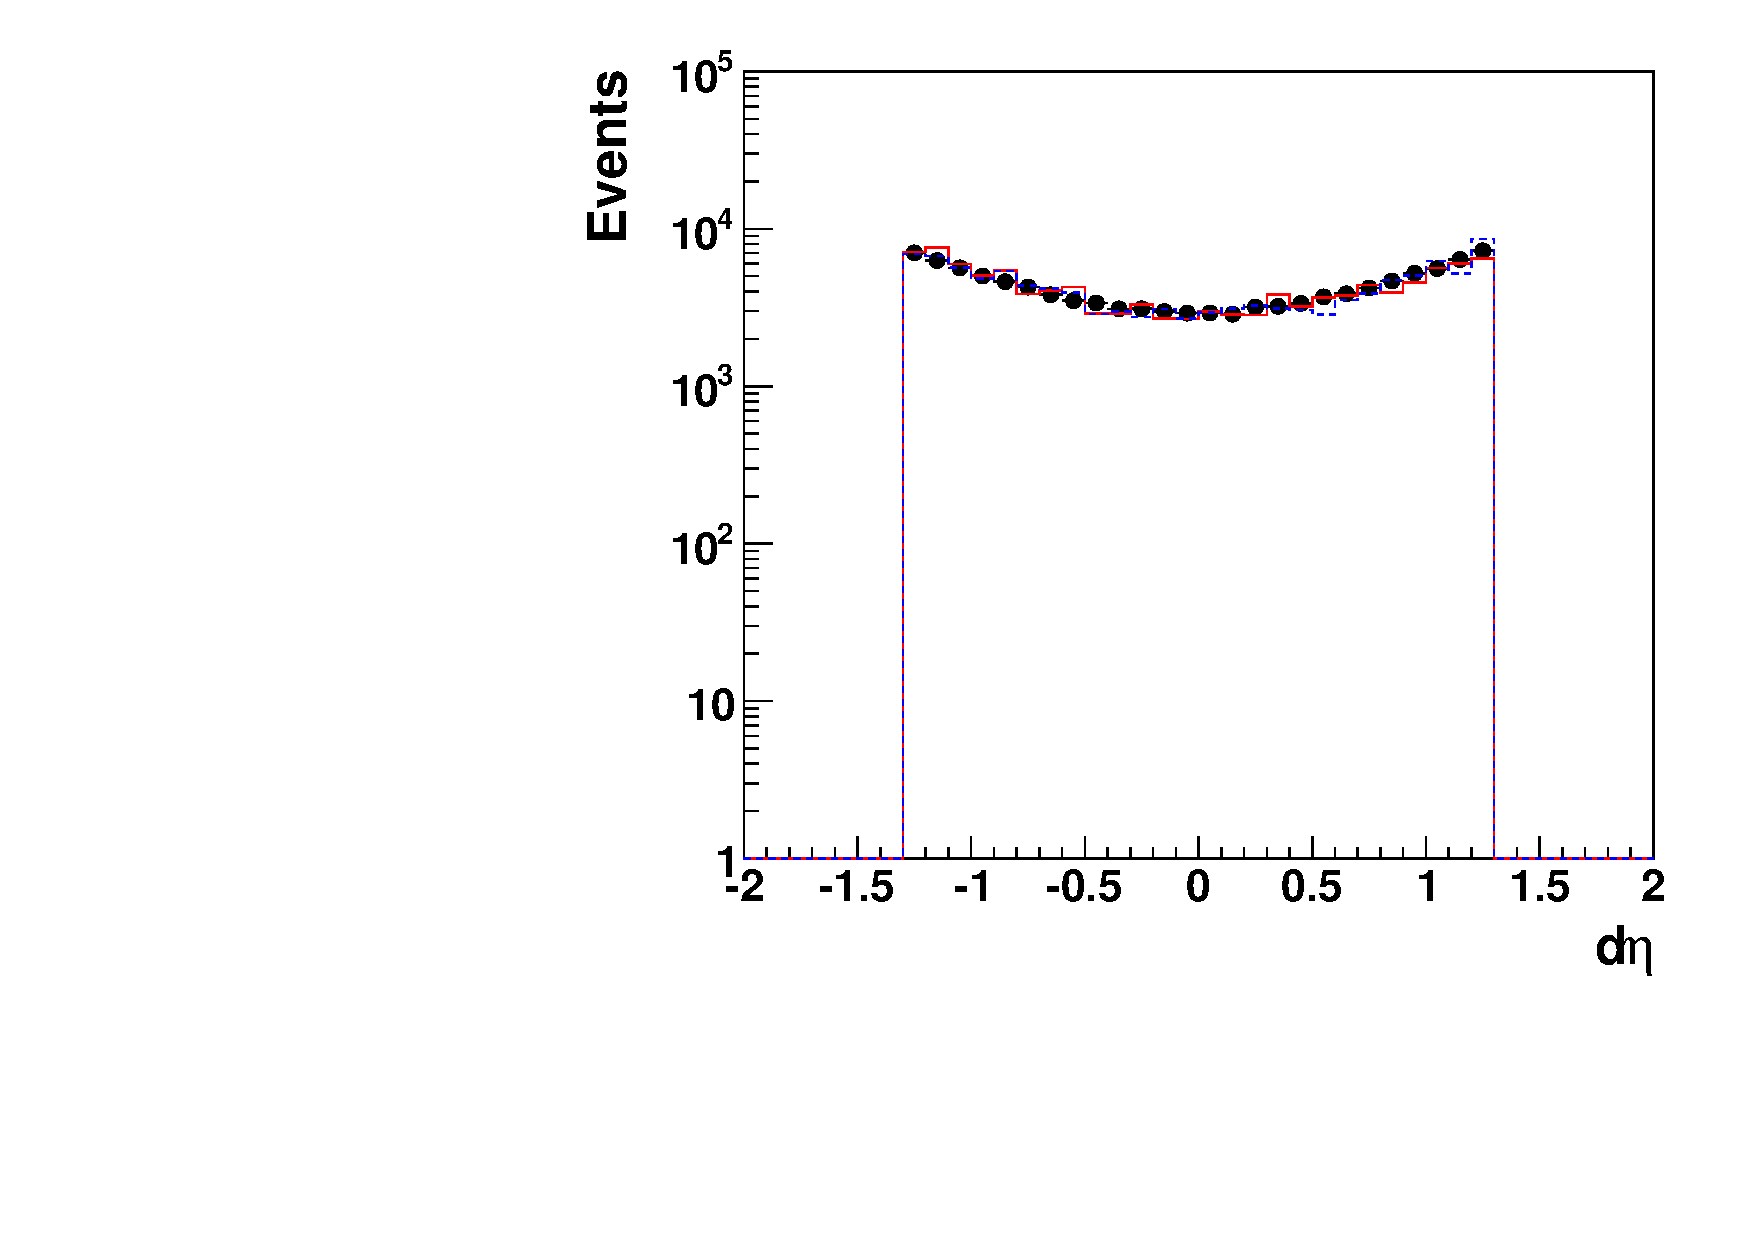
\includegraphics{figs/Data-MC-comparisons/Deta-qVLowP.pdf}} &
     \resizebox{0.5\linewidth}{!}{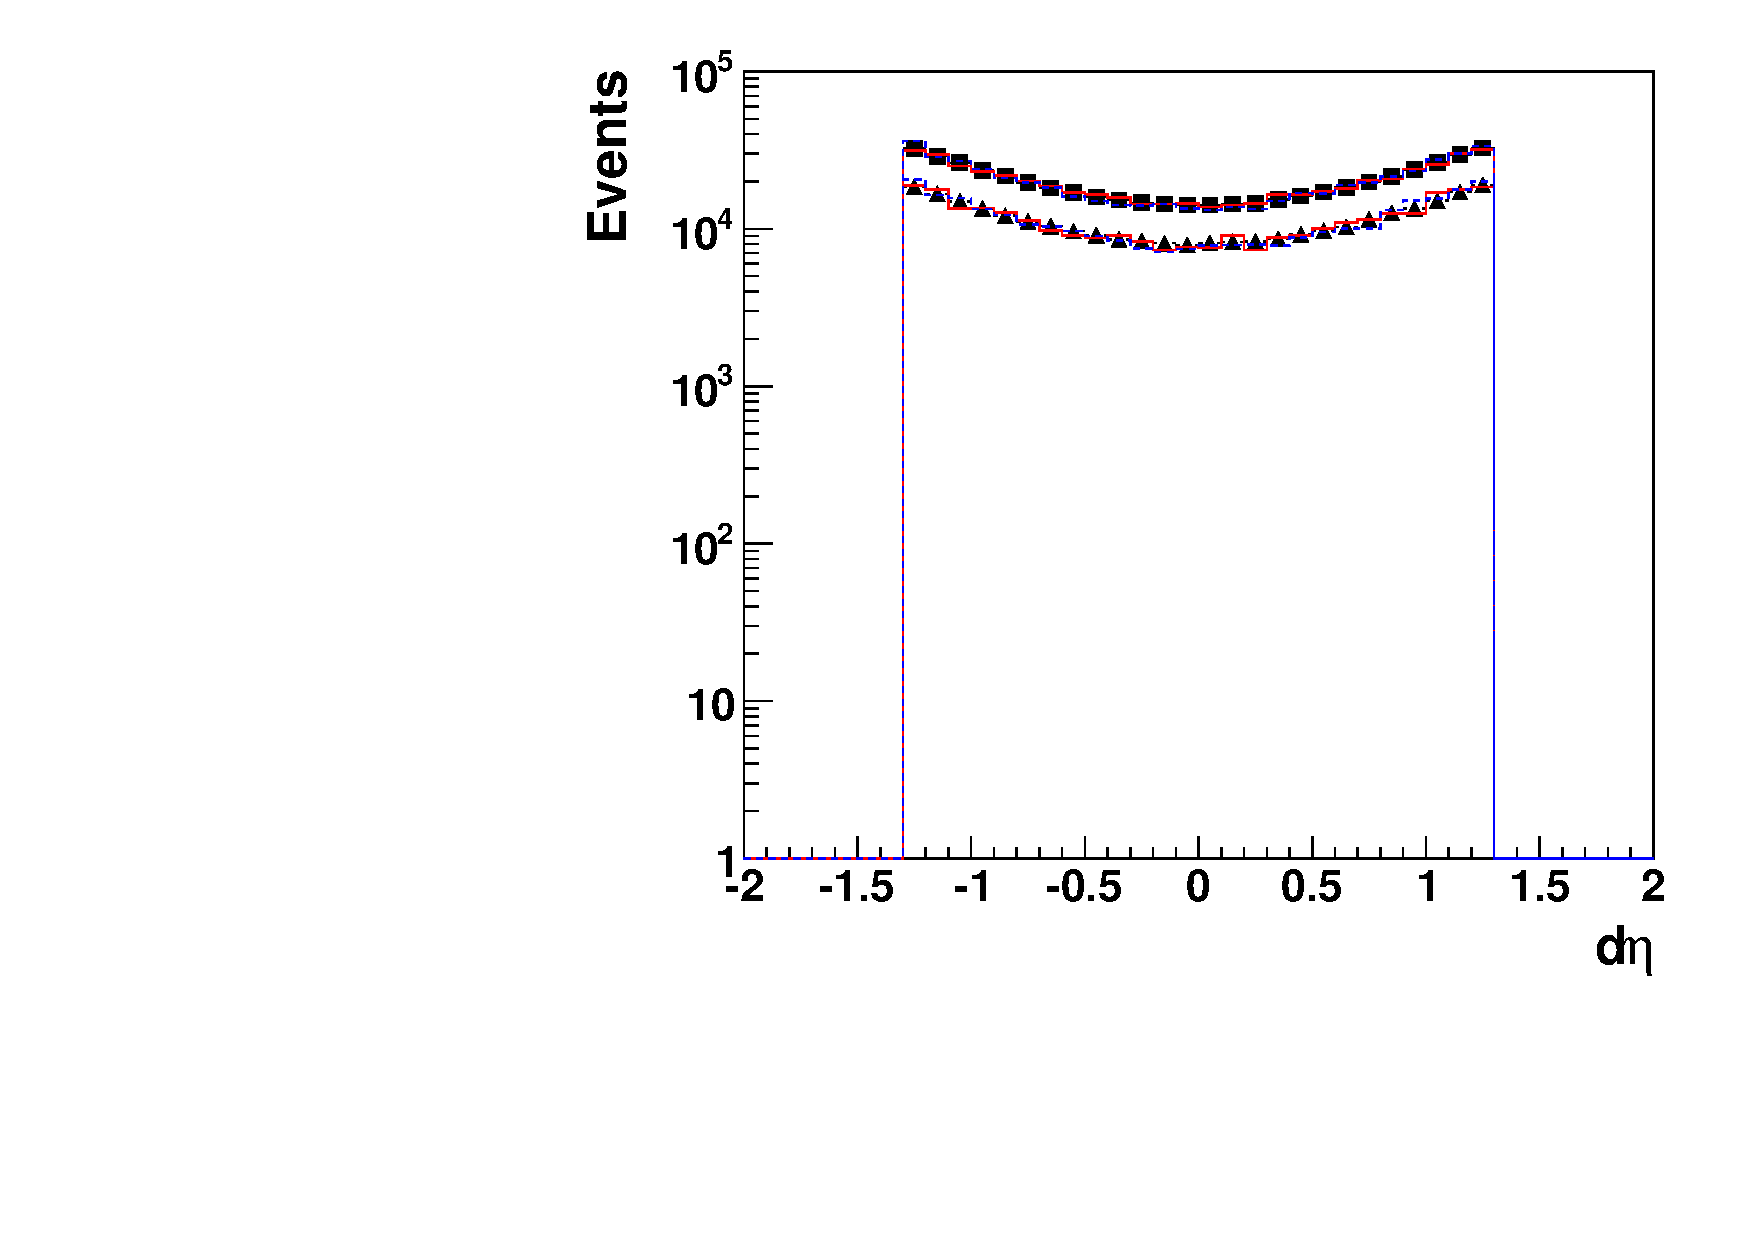
\includegraphics{figs/Data-MC-comparisons/Deta-qVMiumHigh.pdf}} \\
\end{tabular}
  \caption[Delta Eta Single]{Comparisons between data and Monte Carlo
                    for $\Delta\eta$ of the two leading jets of low purity (left) and low-high purity (right) 1-tagged events.
	   The MC is normalized to the number of data events in each category. }
  \label{fig:dySingle}
\end{figure}

\begin{figure}[htb]
\centering
\begin{tabular}{cc}
     \resizebox{0.5\linewidth}{!}{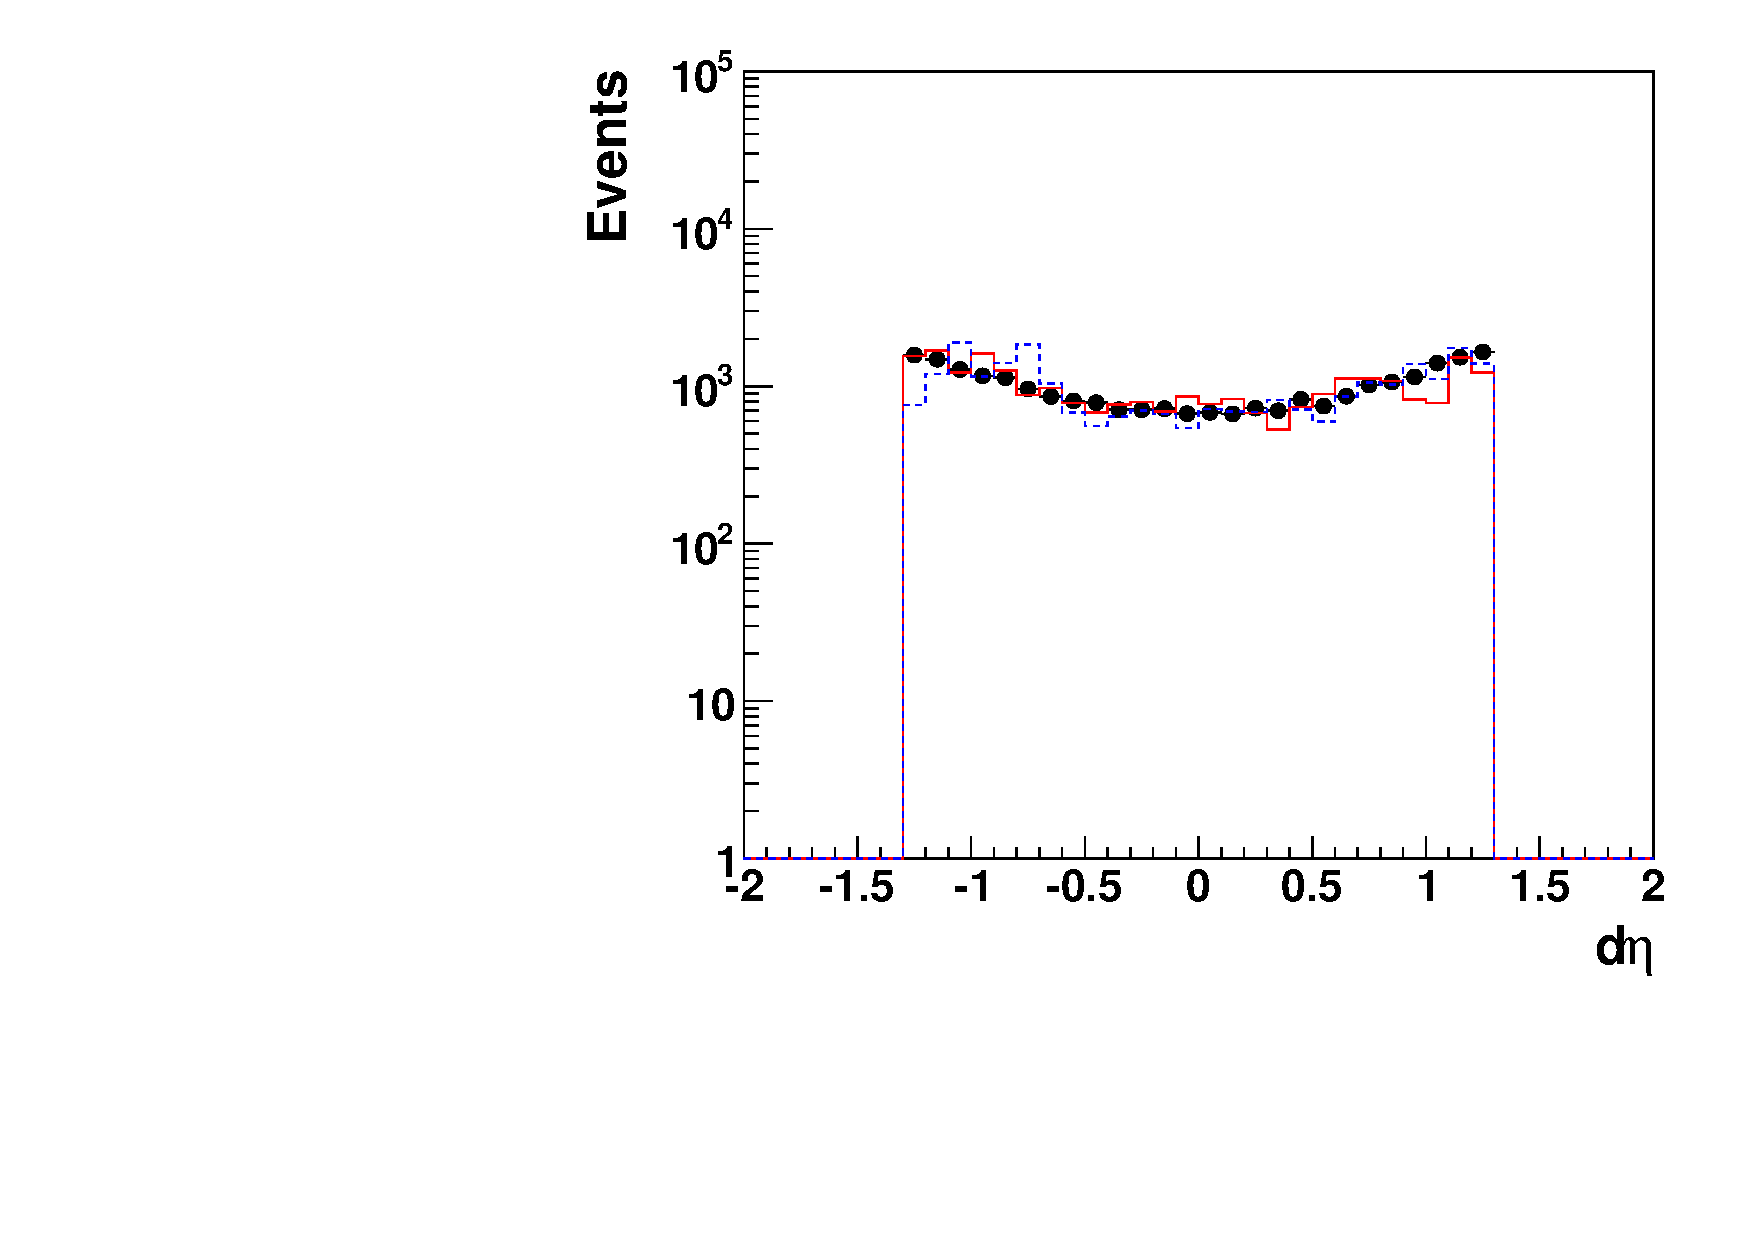
\includegraphics{figs/Data-MC-comparisons/Deta-VVLowP.pdf}} &
     \resizebox{0.5\linewidth}{!}{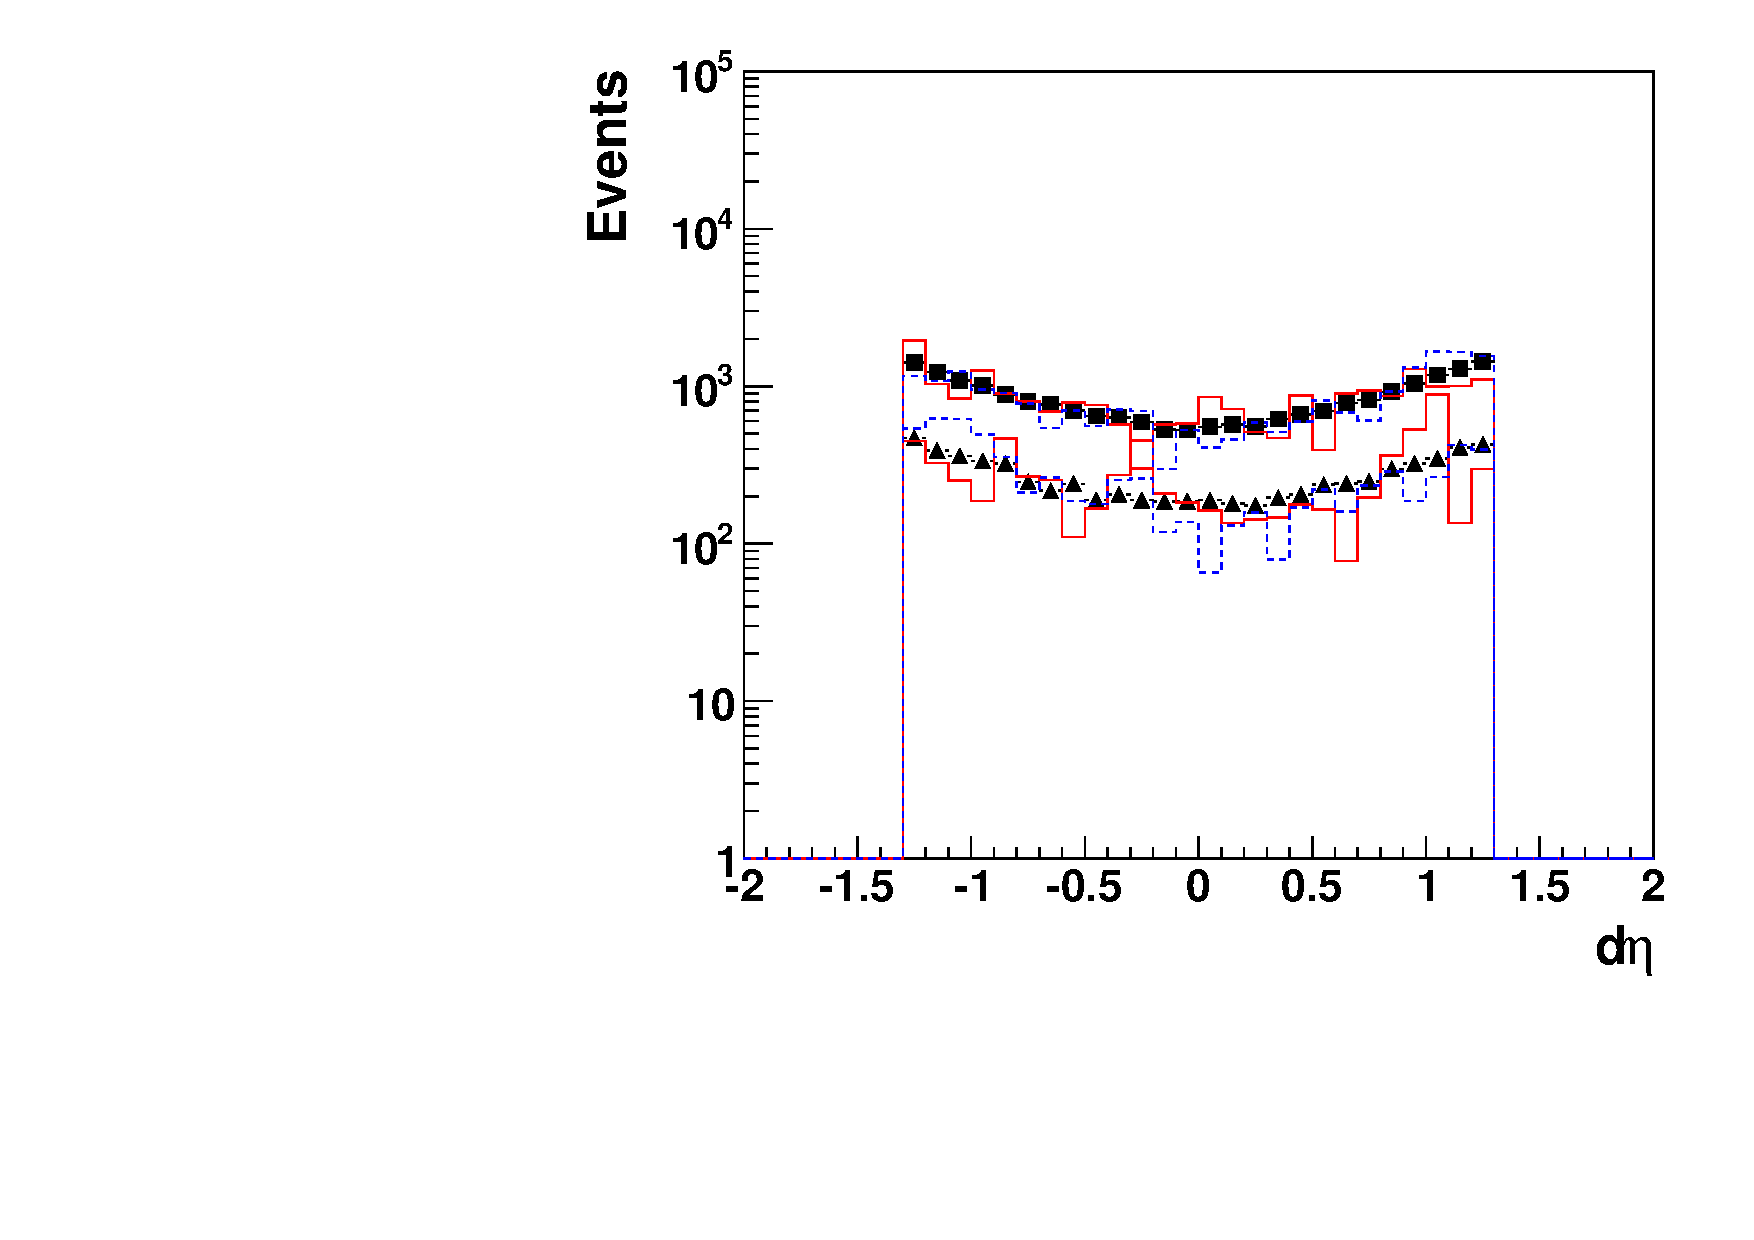
\includegraphics{figs/Data-MC-comparisons/Deta-VVMiumHigh.pdf}} \\
\end{tabular}
  \caption[Delta Eta Double]{Comparisons between data and Monte Carlo
                     for $\Delta\eta$ of the two leading jets of low purity (left) and low-high purity (right) 2-tagged events. The MC is normalized to the number of data events in each category. }
  \label{fig:dyDouble}
\end{figure}


\newpage
\begin{figure}[htb]
\centering
\begin{tabular}{cc}
     \resizebox{0.5\linewidth}{!}{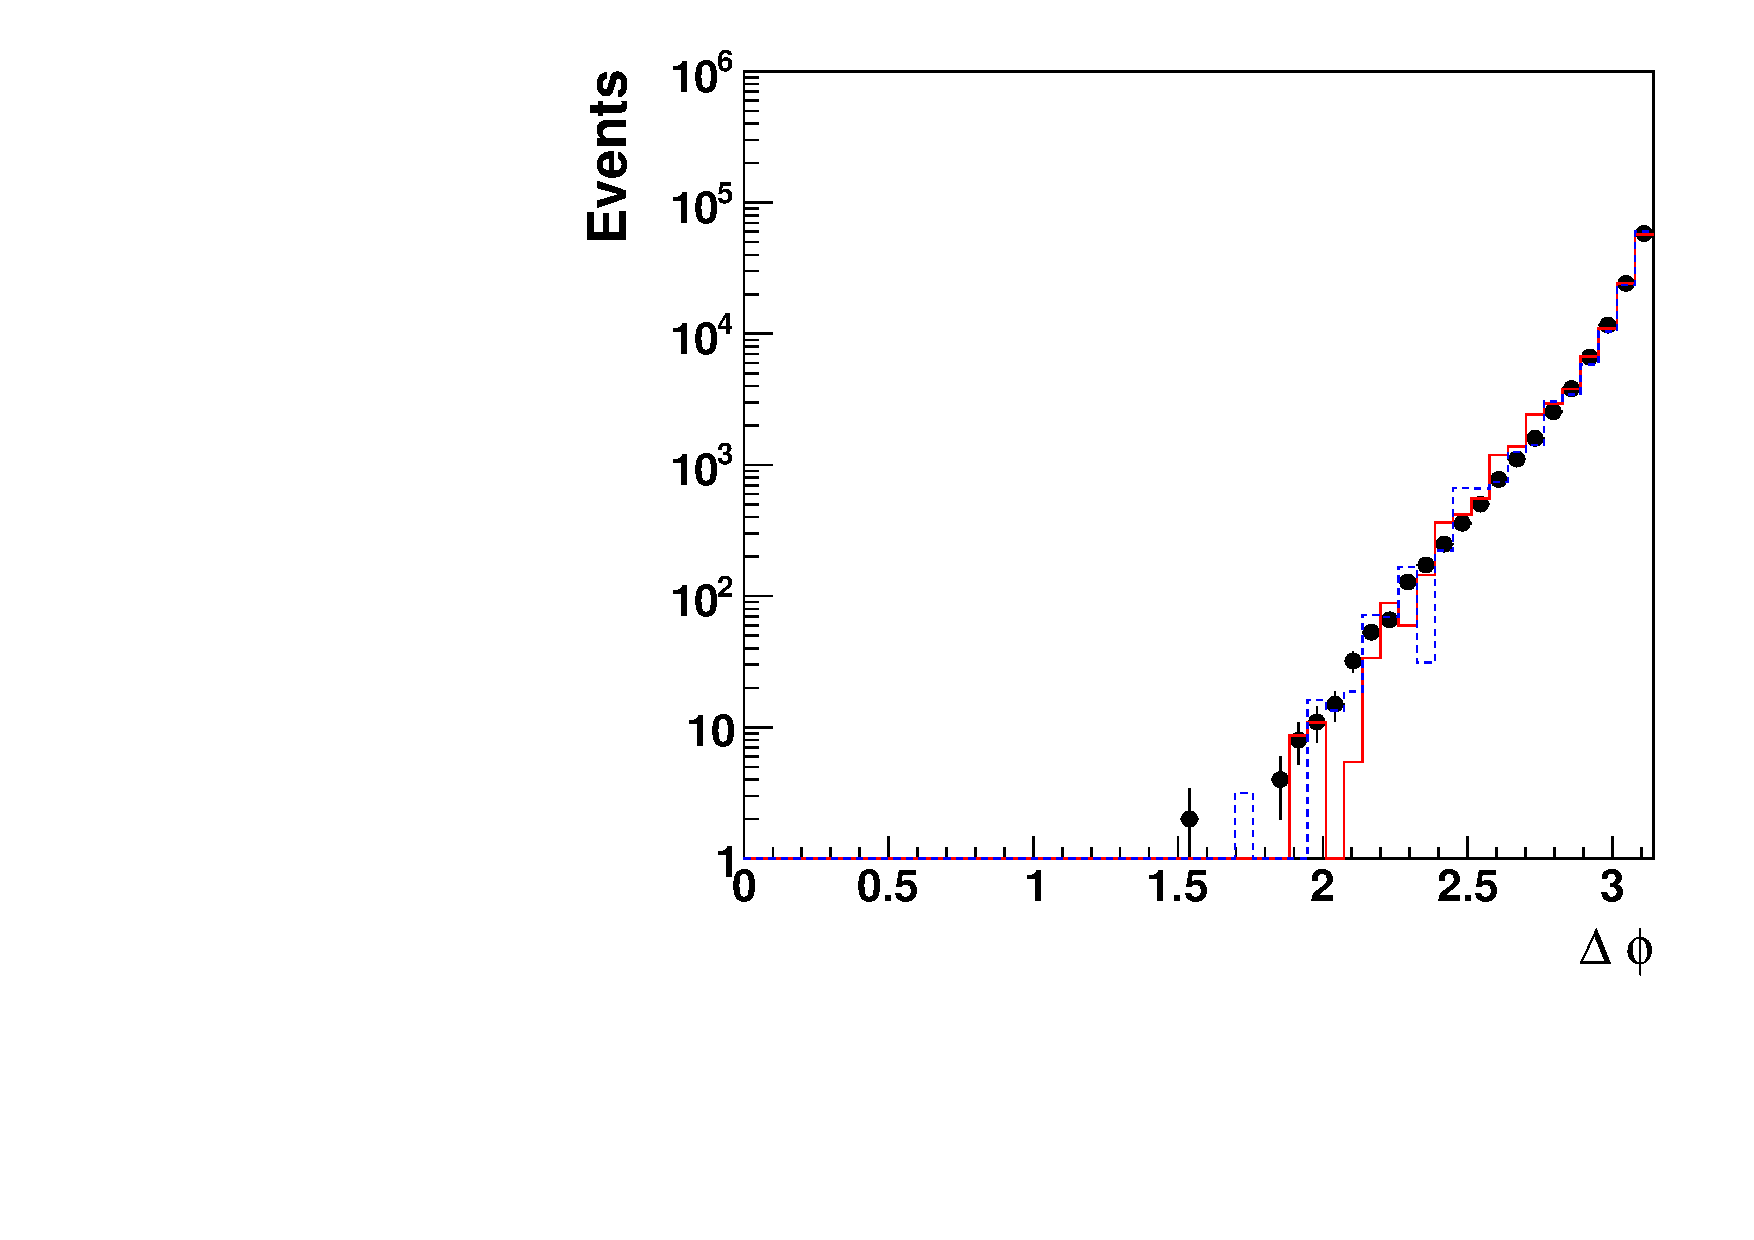
\includegraphics{figs/Data-MC-comparisons/Dphi-qVLowP.pdf}} &
     \resizebox{0.5\linewidth}{!}{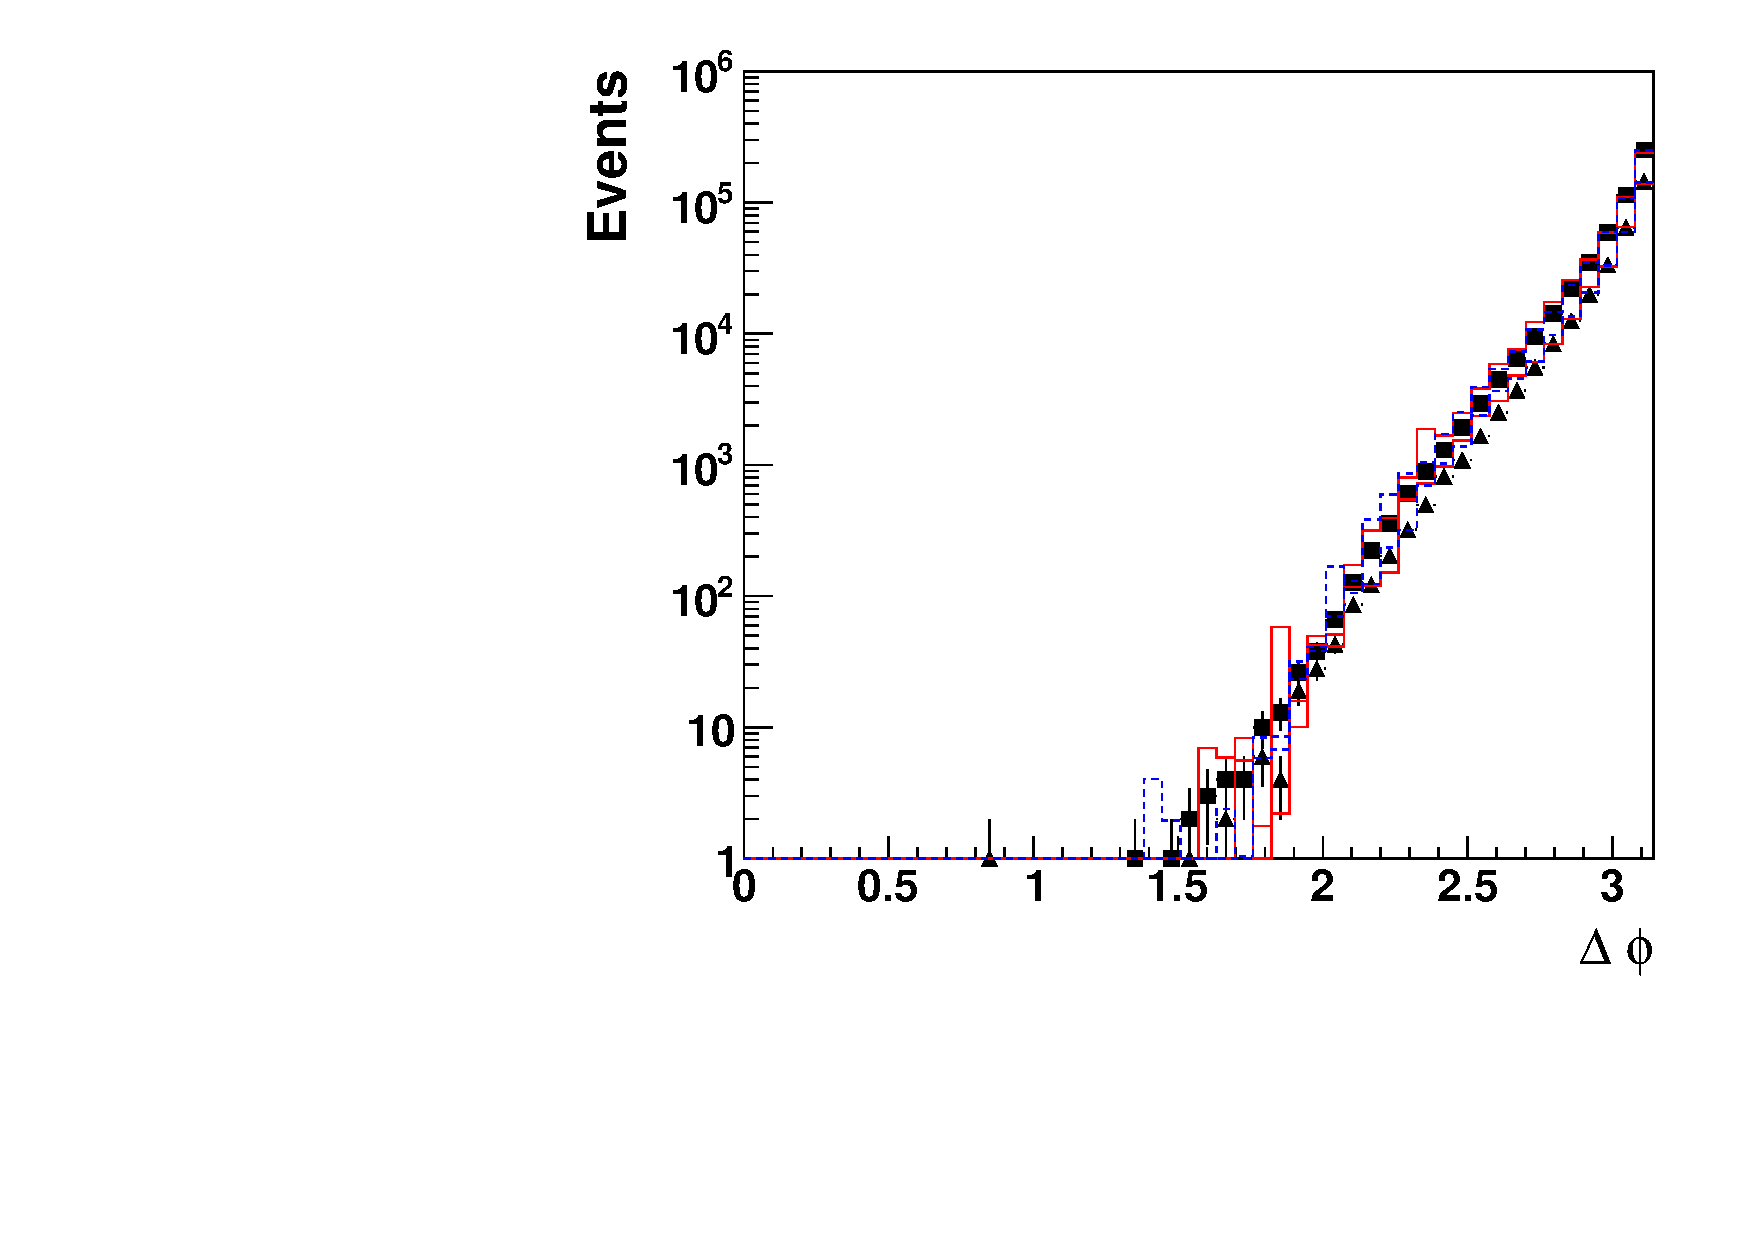
\includegraphics{figs/Data-MC-comparisons/Dphi-qVMiumHigh.pdf}} \\
\end{tabular}
  \caption[Delta Eta Single]{Comparisons between data and Monte Carlo
                    for $\Delta\phi$ of the two leading jets of low purity (left) and low-high purity (right) 1-tagged events.
	   The MC is normalized to the number of data events in each category. }
  \label{fig:dphiSingle}
\end{figure}

\begin{figure}[htb]
\centering
\begin{tabular}{cc}
     \resizebox{0.5\linewidth}{!}{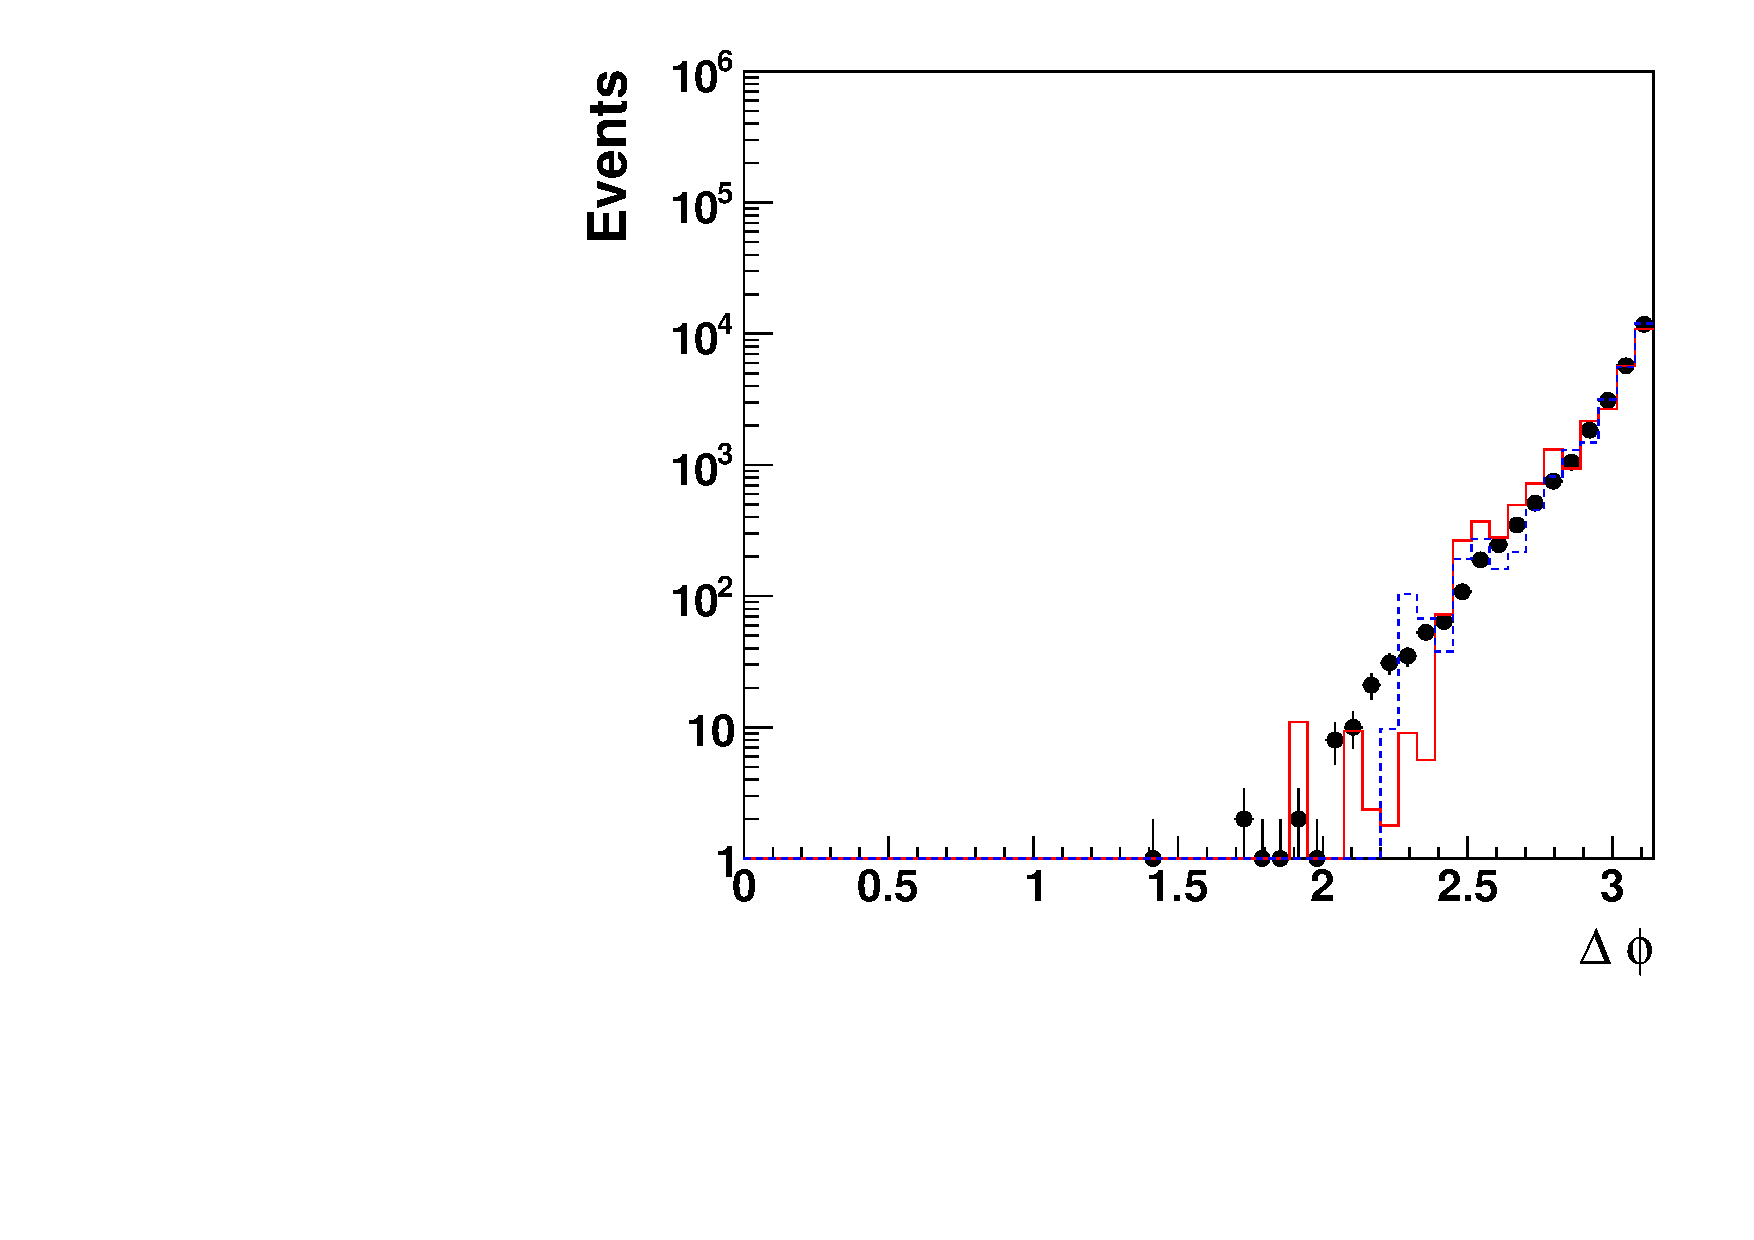
\includegraphics{figs/Data-MC-comparisons/Dphi-VVLowP.pdf}} &
     \resizebox{0.5\linewidth}{!}{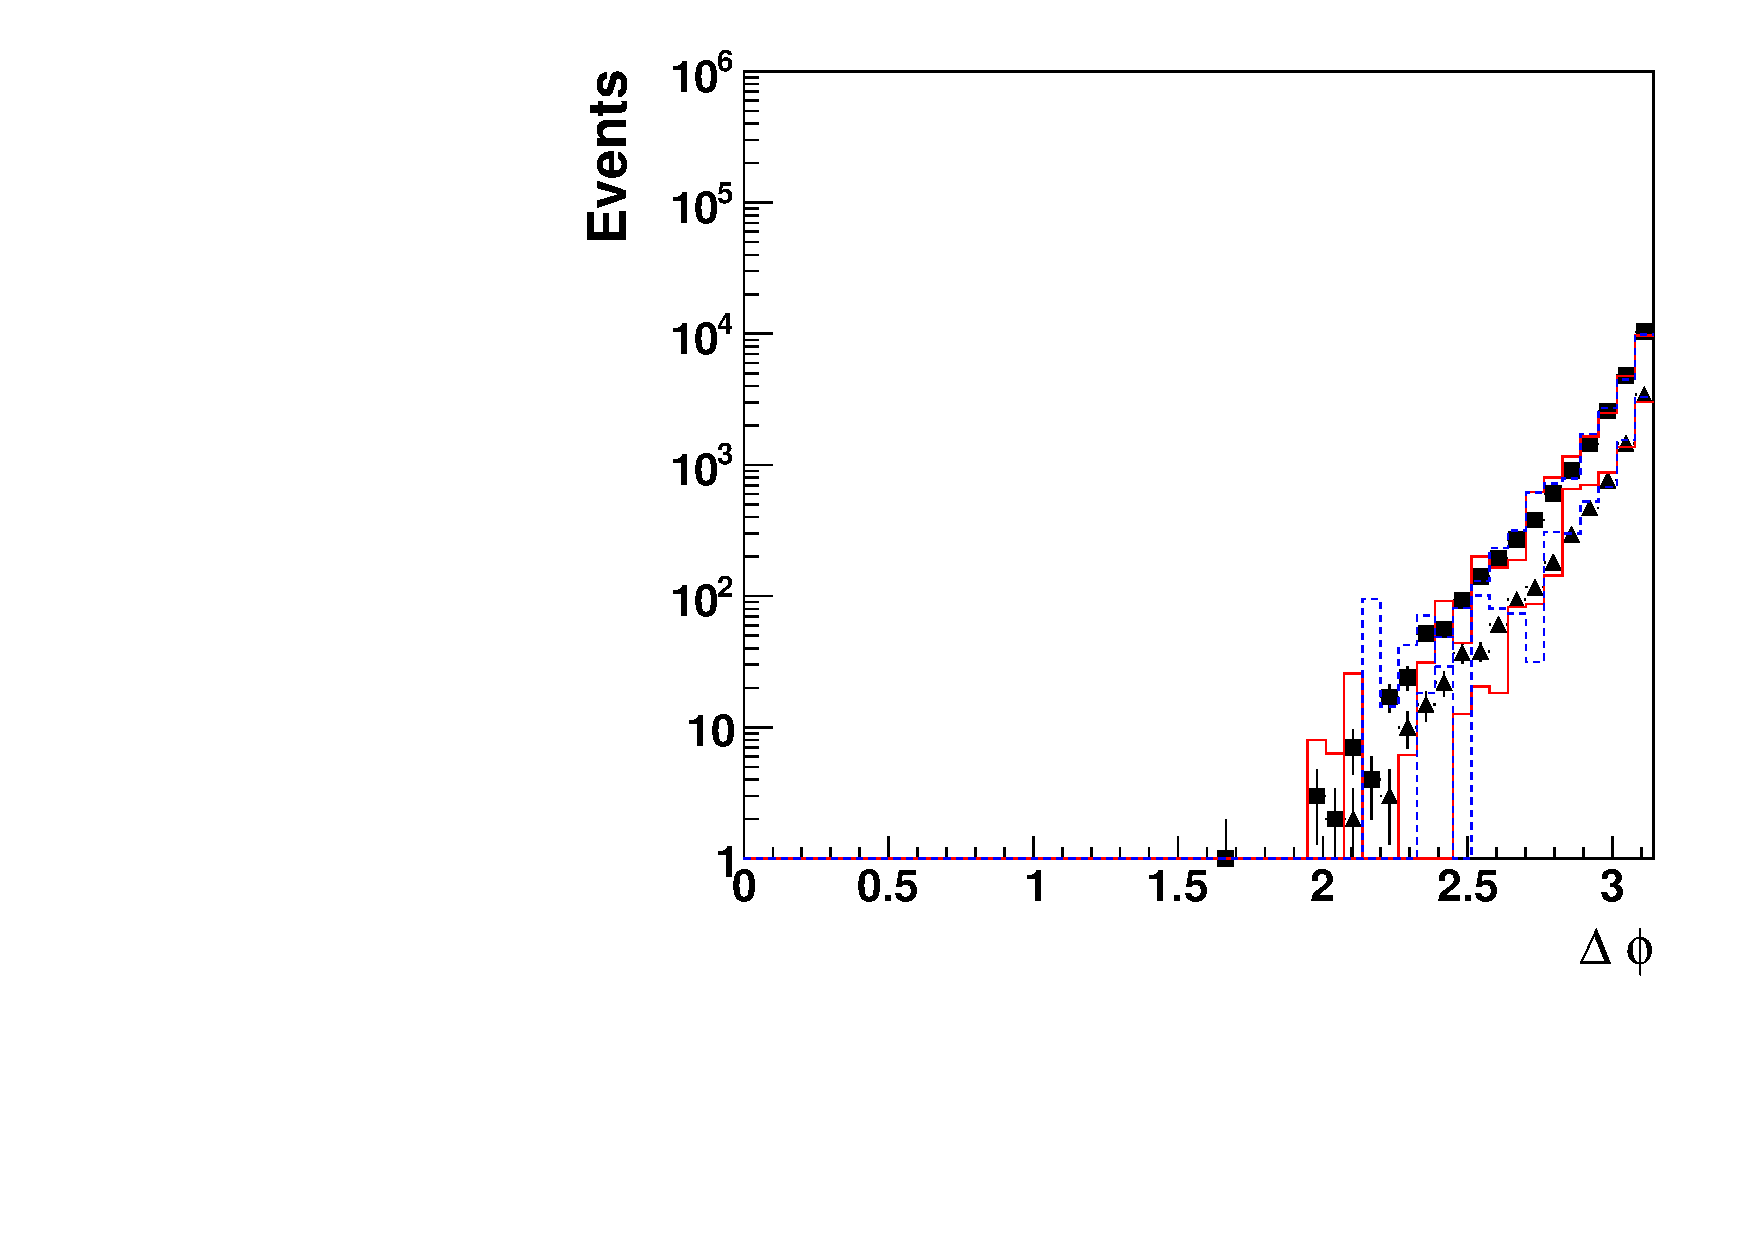
\includegraphics{figs/Data-MC-comparisons/Dphi-VVMiumHigh.pdf}} \\
\end{tabular}
  \caption[Delta Eta Double]{Comparisons between data and Monte Carlo
                     for $\Delta\phi$ of the two leading jets of low purity (left) and low-high purity (right) 2-tagged events. The MC is normalized to the number of data events in each category. }
  \label{fig:dphiDouble}
\end{figure}

\newpage

\begin{figure}[htb]
\centering
\begin{tabular}{cc}
     \resizebox{0.5\linewidth}{!}{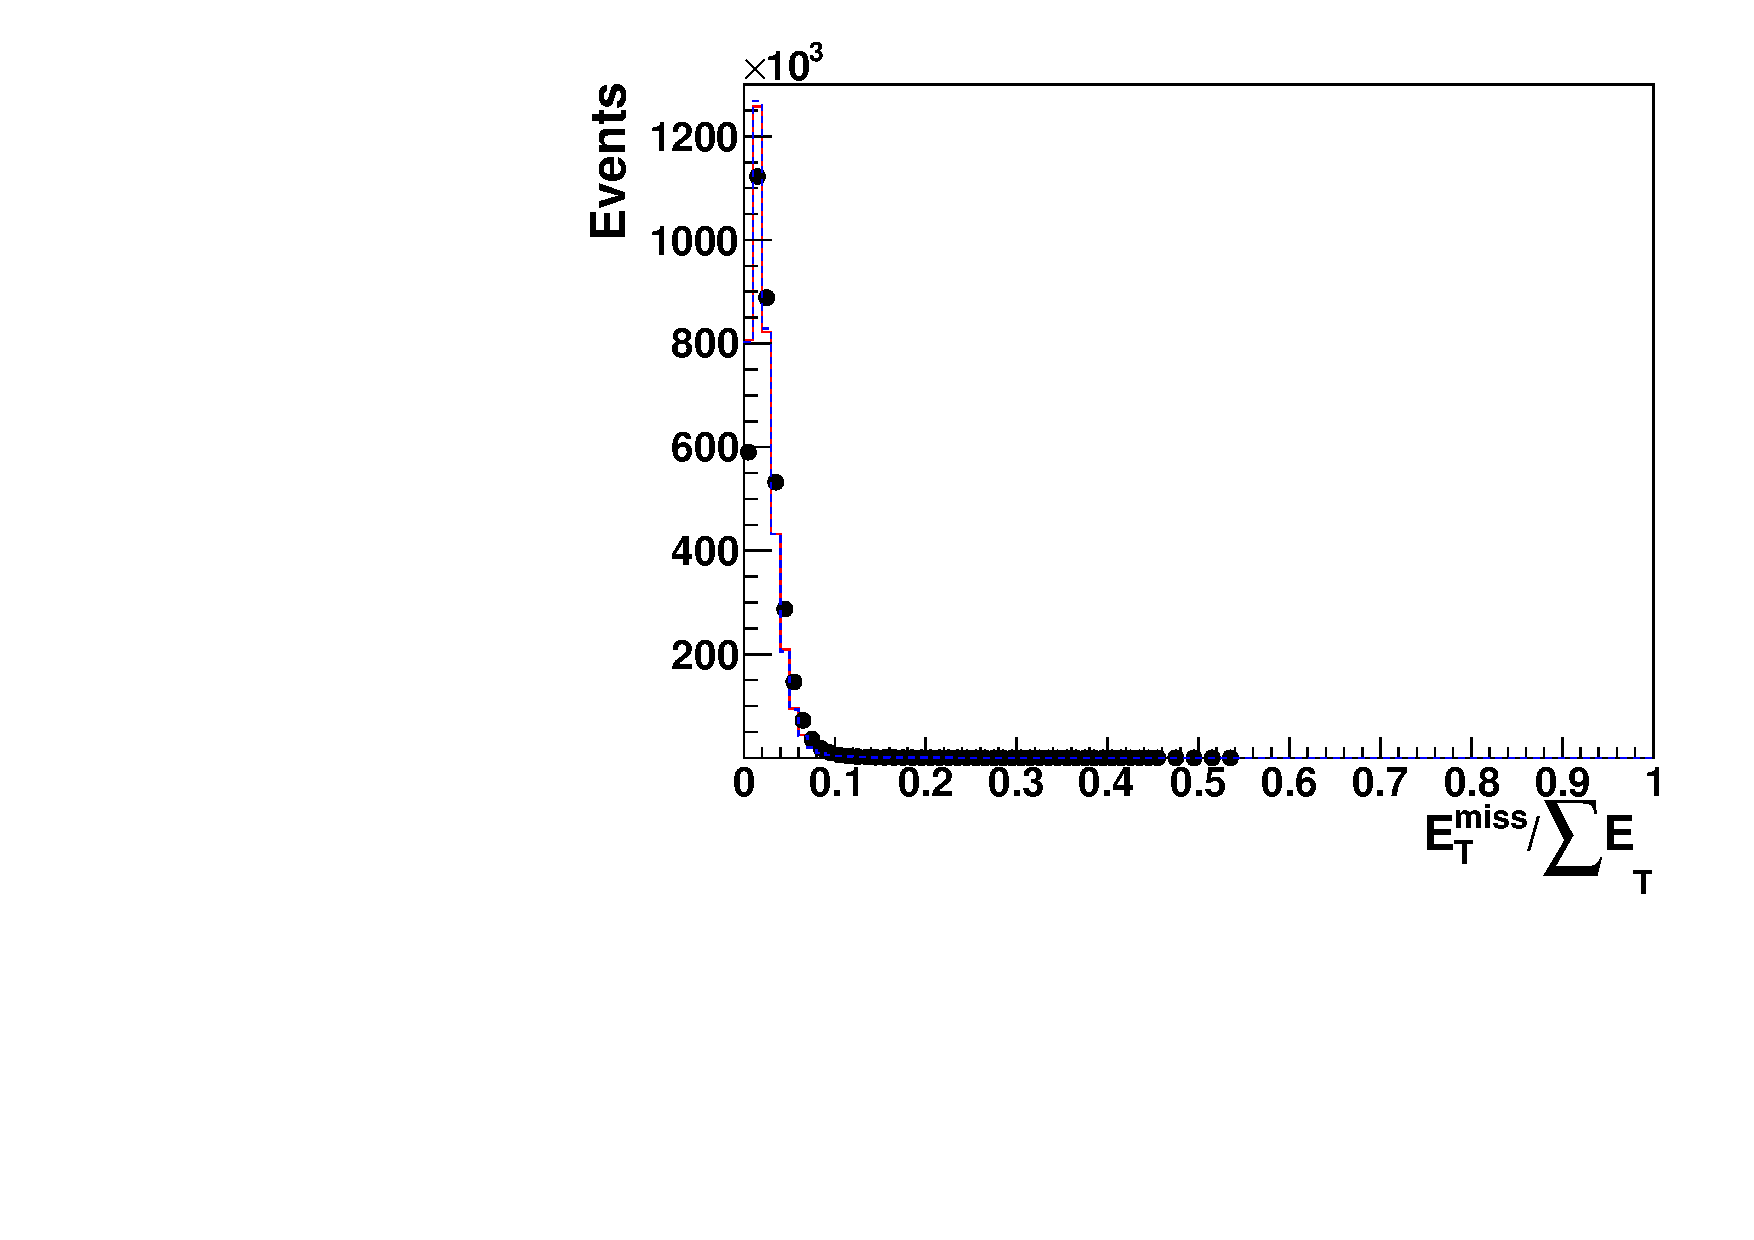
\includegraphics{figs/Data-MC-comparisons/etsumEt.pdf}} &
     \resizebox{0.5\linewidth}{!}{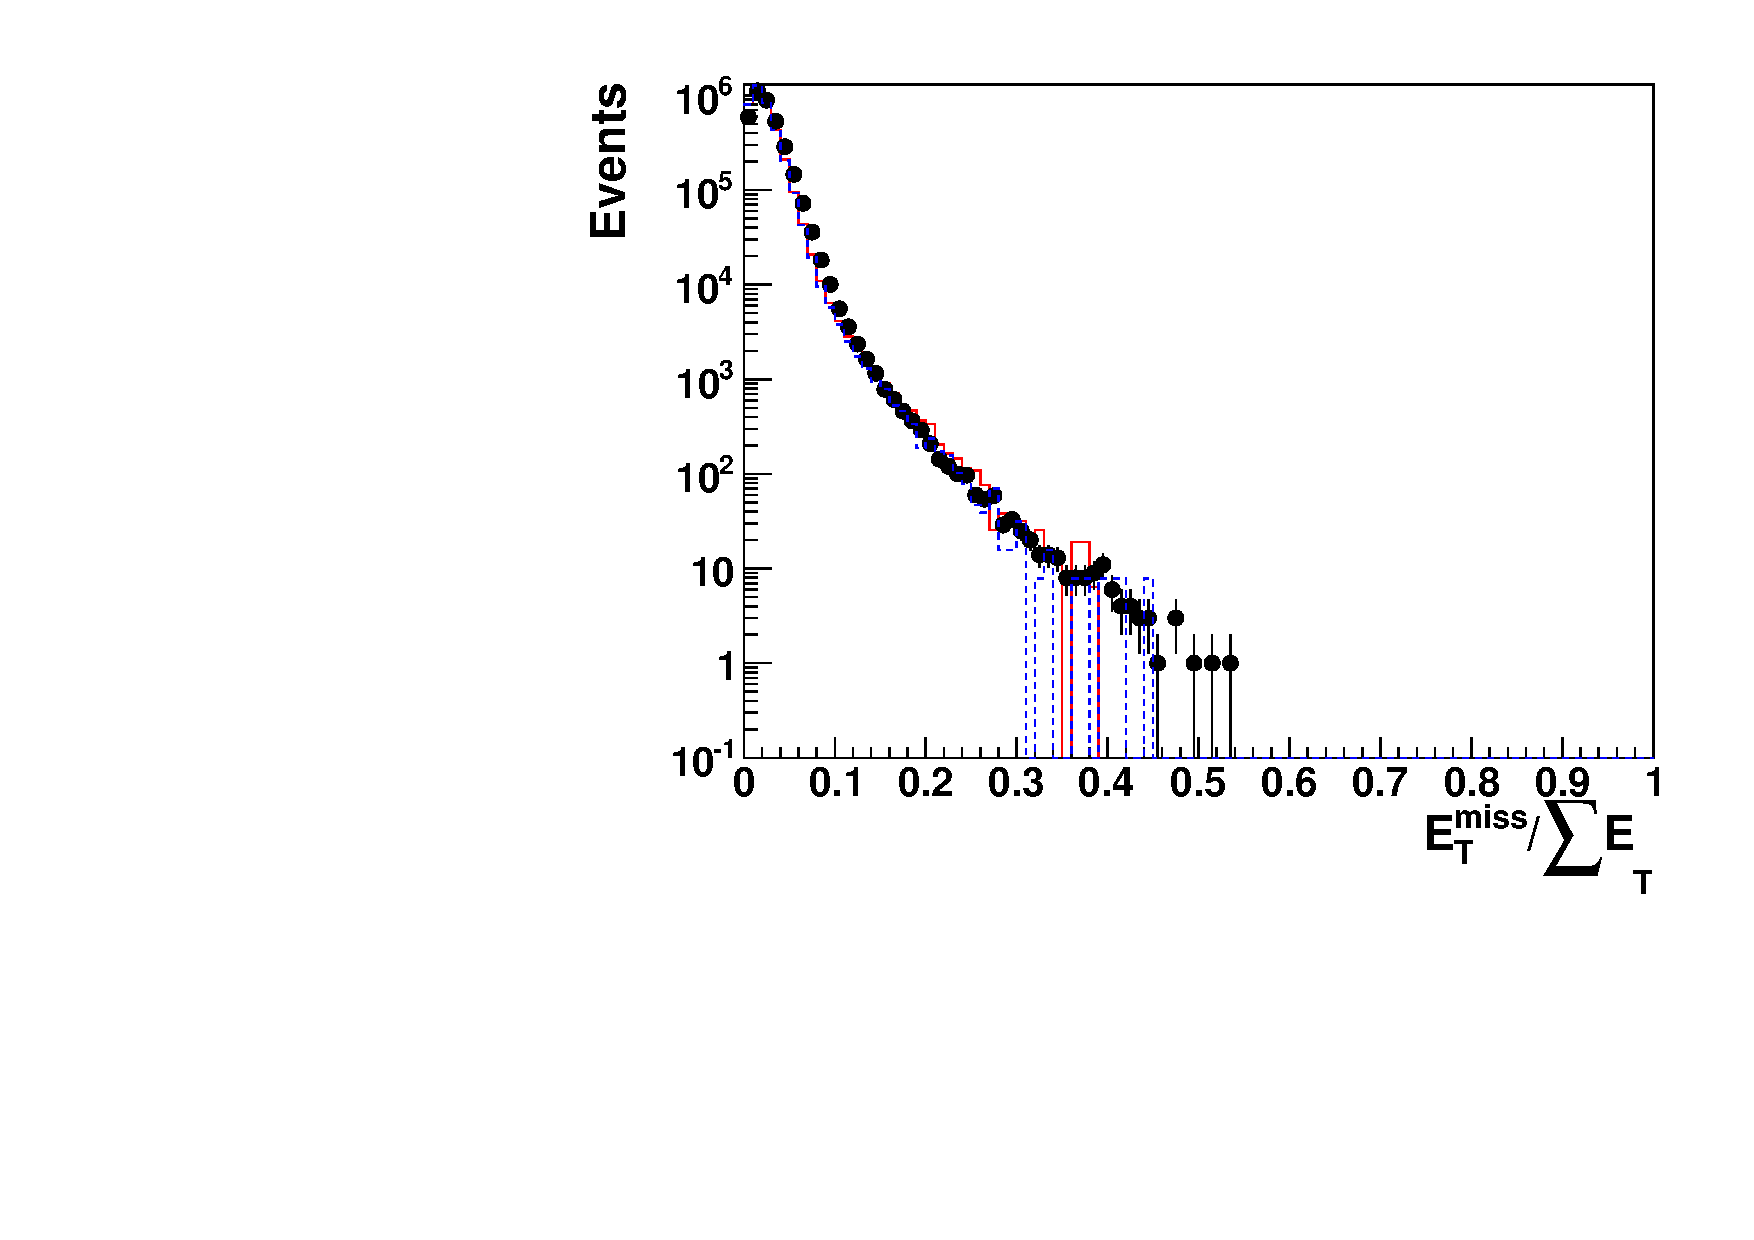
\includegraphics{figs/Data-MC-comparisons/etsumEtlog.pdf}} \\
\end{tabular}
  \caption[Leading two jets mass drop]{Comparisons between data and Monte Carlo for $E_{T}^{miss}/\sum E_{T}$ 
	   The MC is normalized to the number of data events. Plot on the right is the log scale plot. (The plot includes only a subset of the full data sample.)}
  \label{fig:metSumPtSingle}
\end{figure}

%\begin{figure}[htb]
%\centering
%\begin{tabular}{cc}
%     \resizebox{0.5\linewidth}{!}{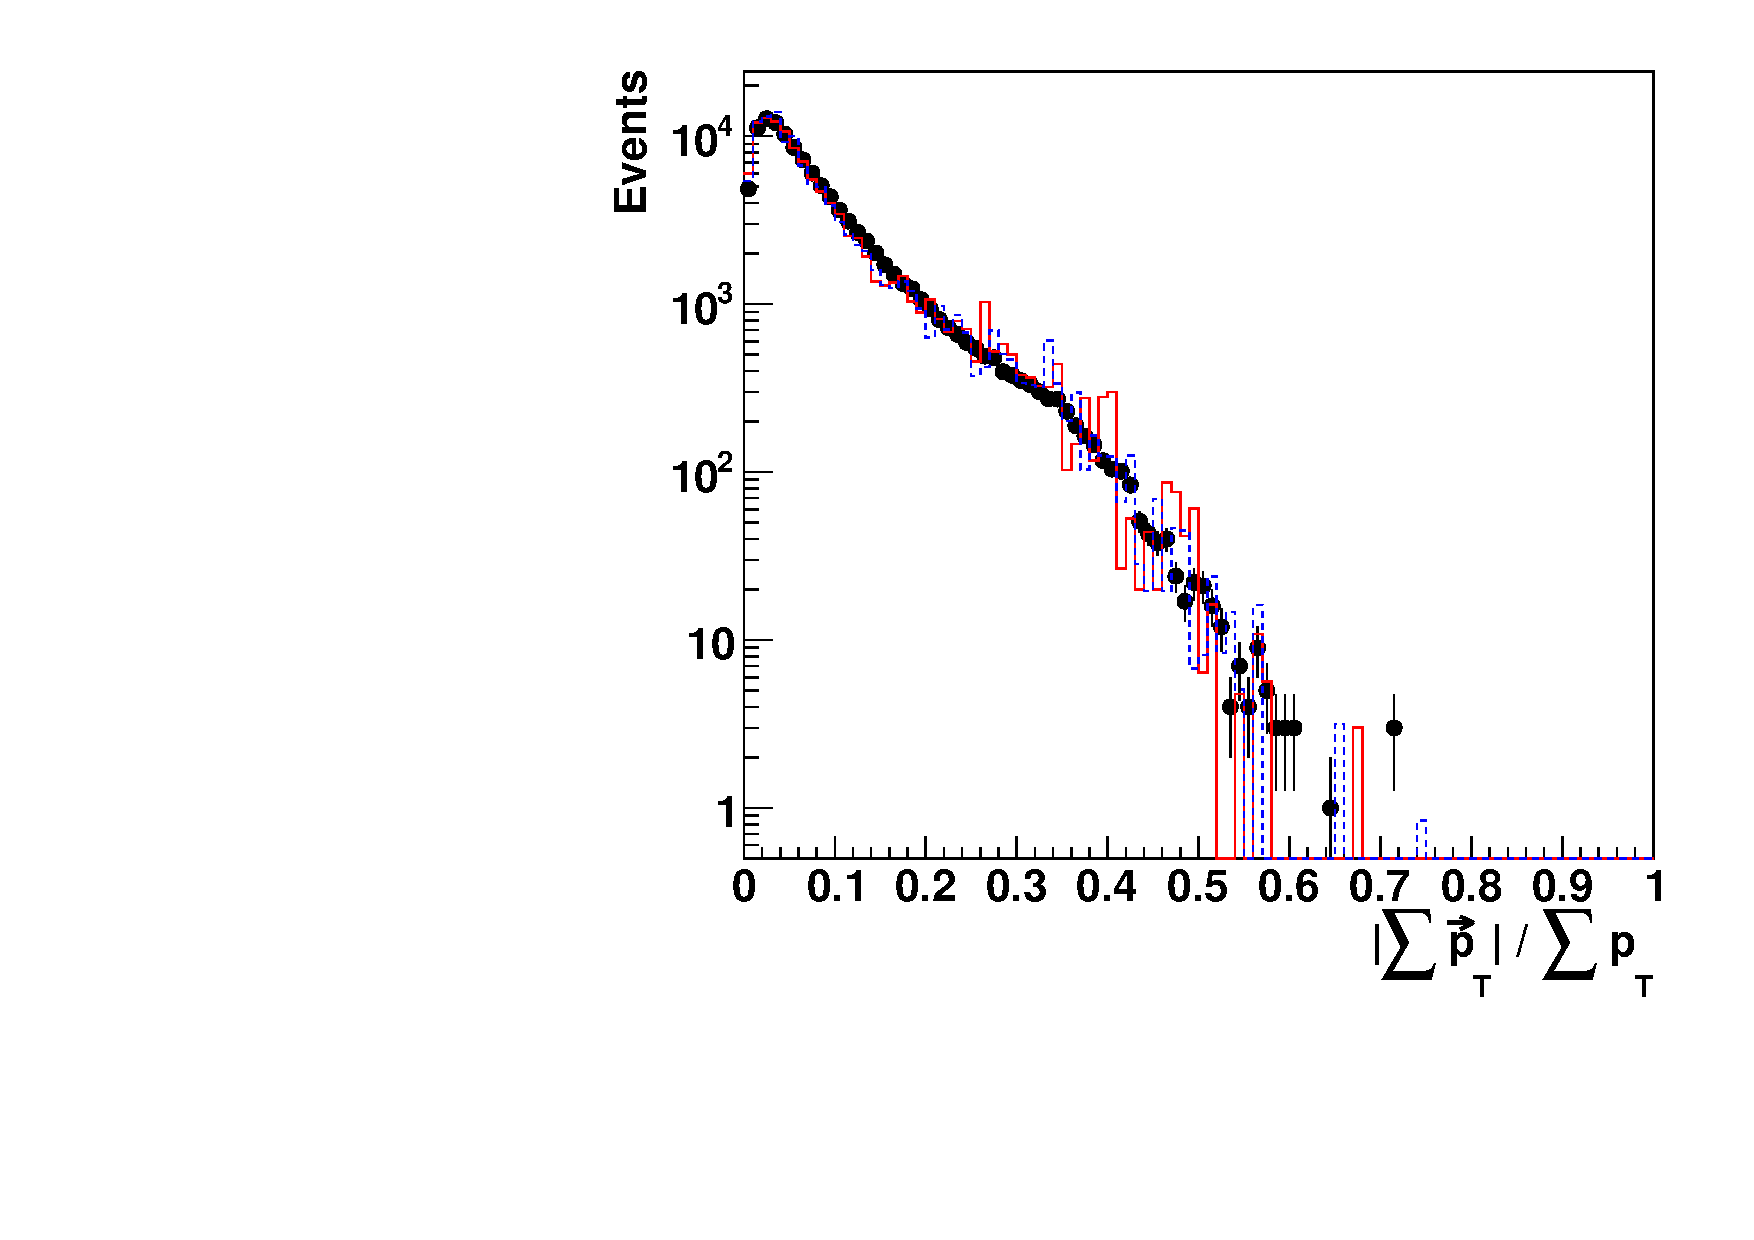
\includegraphics{figs/Data-MC-comparisons/PTVSPT-qVLowP.pdf}} &
%     \resizebox{0.5\linewidth}{!}{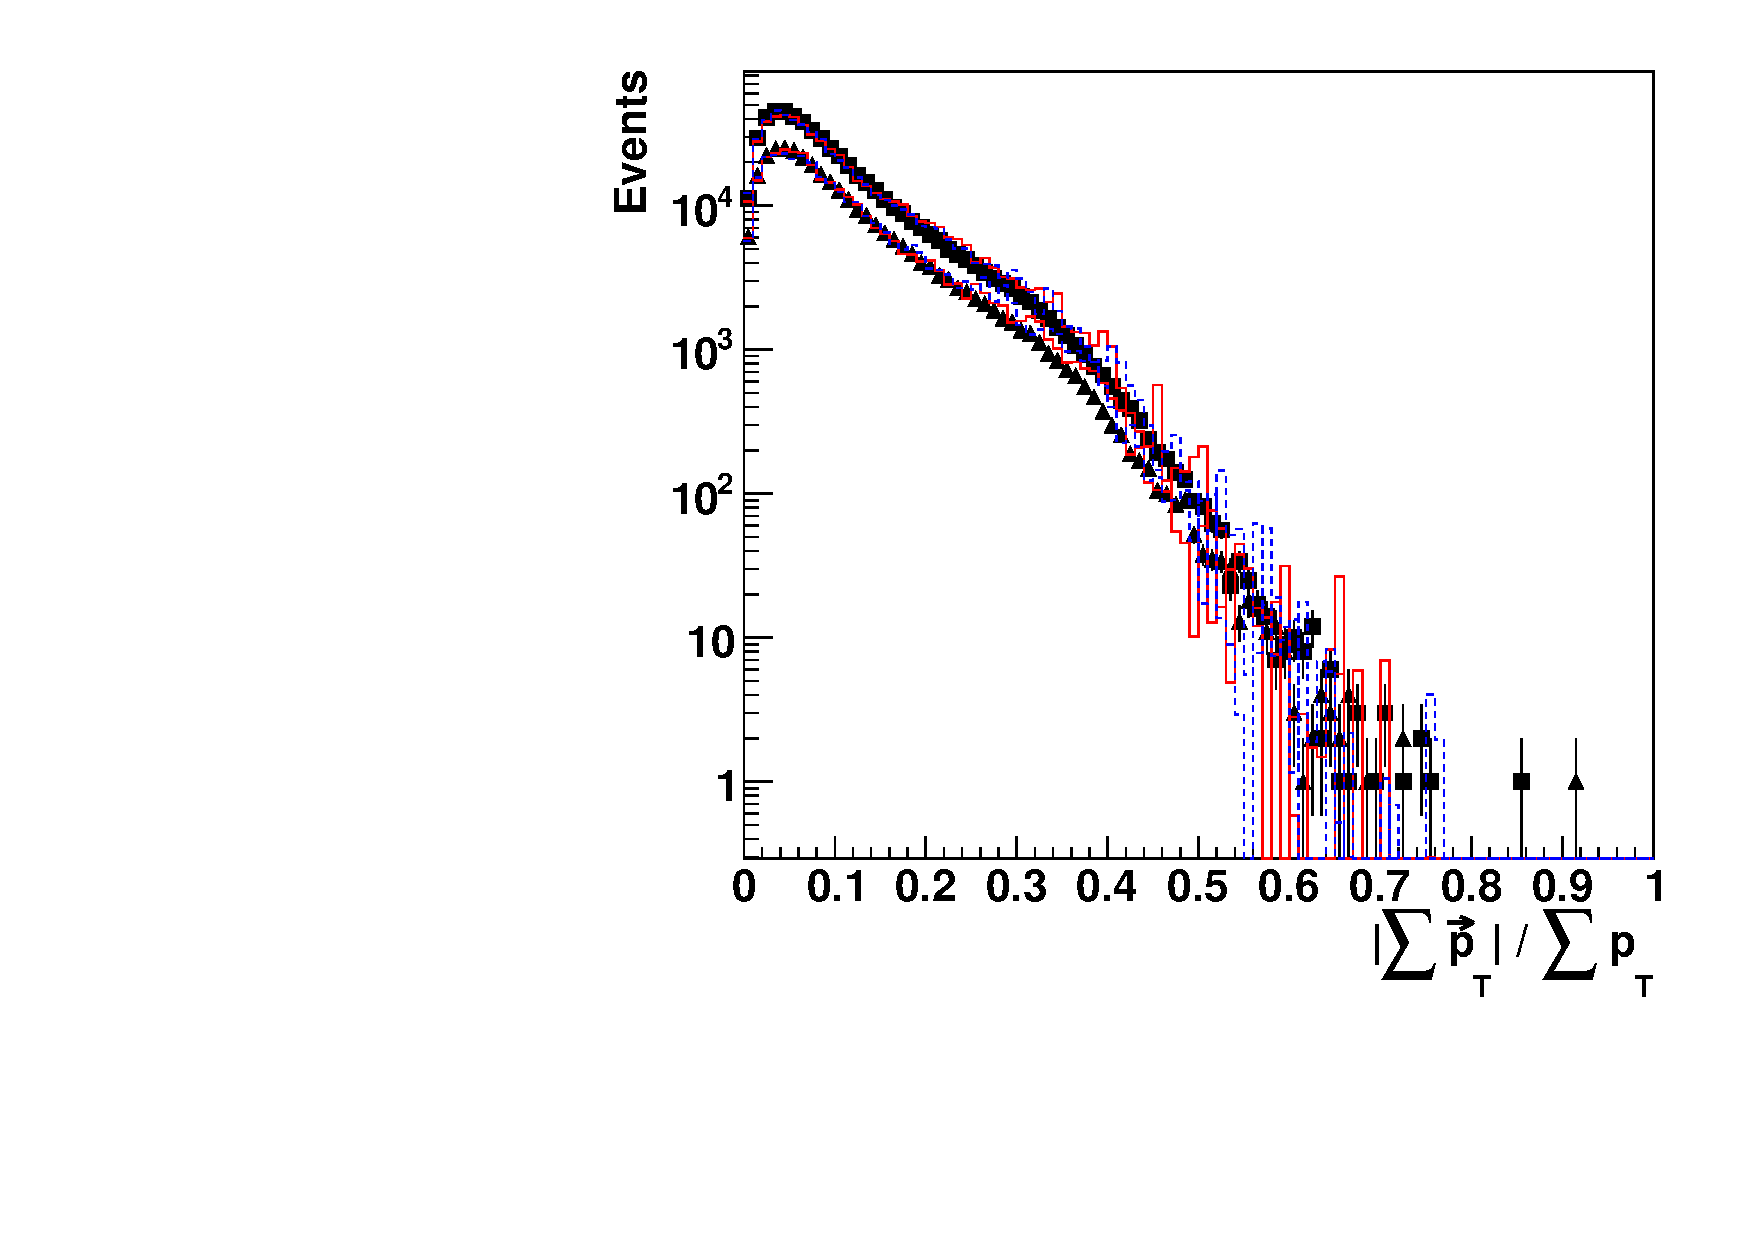
\includegraphics{figs/Data-MC-comparisons/PTVSPT-qVMiumHigh.pdf}} \\
%\end{tabular}
%  \caption[Delta Eta Single]{Comparisons between data and Monte Carlo
%                    for $|\sum{\vec{p}_{T}}| / \sum{p_{T}}$ of the two leading jets of low purity (left) and low-high purity (right) 1-tagged events.
%	   The MC is normalized to the number of data events in each category. }
%  \label{fig:metSumPtSingle}
%\end{figure}

%\begin{figure}[htb]
%\centering
%\begin{tabular}{cc}
%     \resizebox{0.5\linewidth}{!}{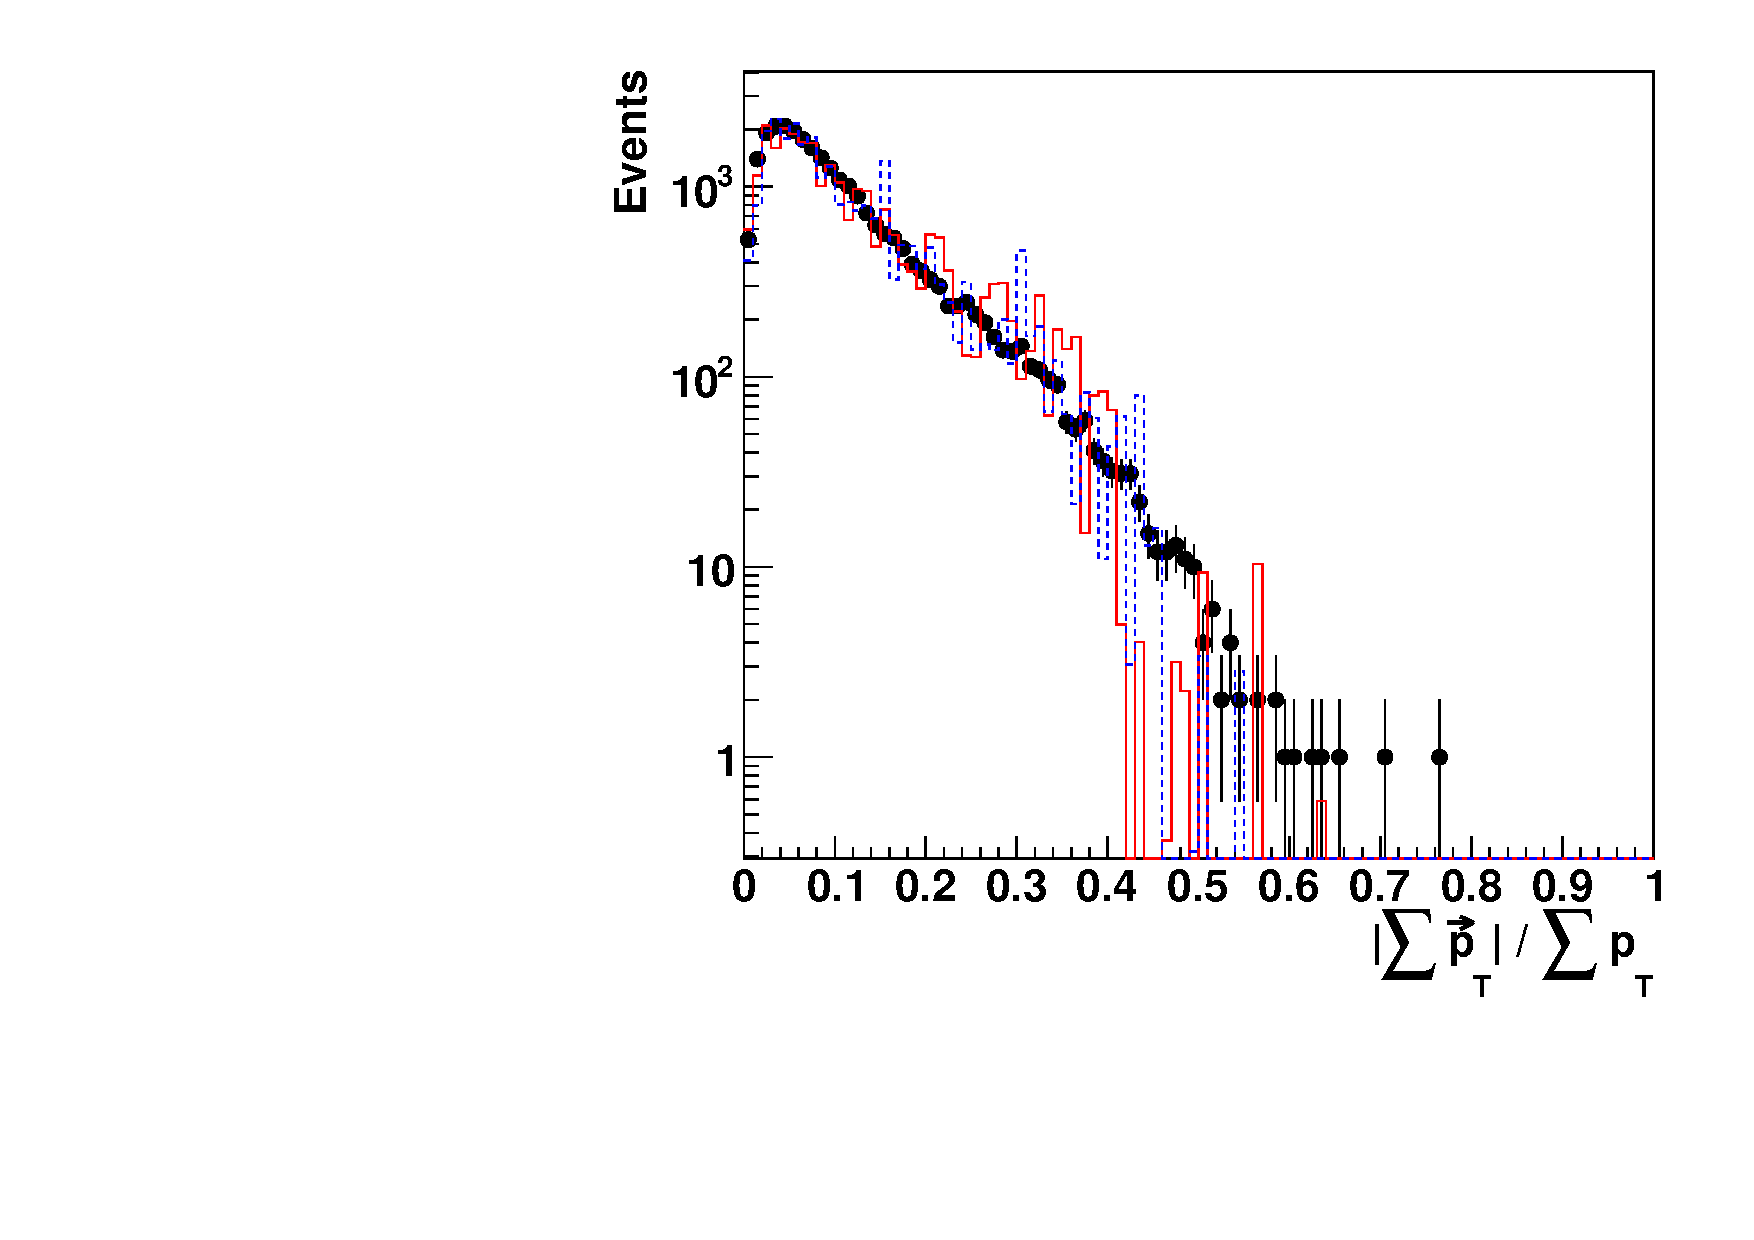
\includegraphics{figs/Data-MC-comparisons/PTVSPT-VVLowP.pdf}} &
%     \resizebox{0.5\linewidth}{!}{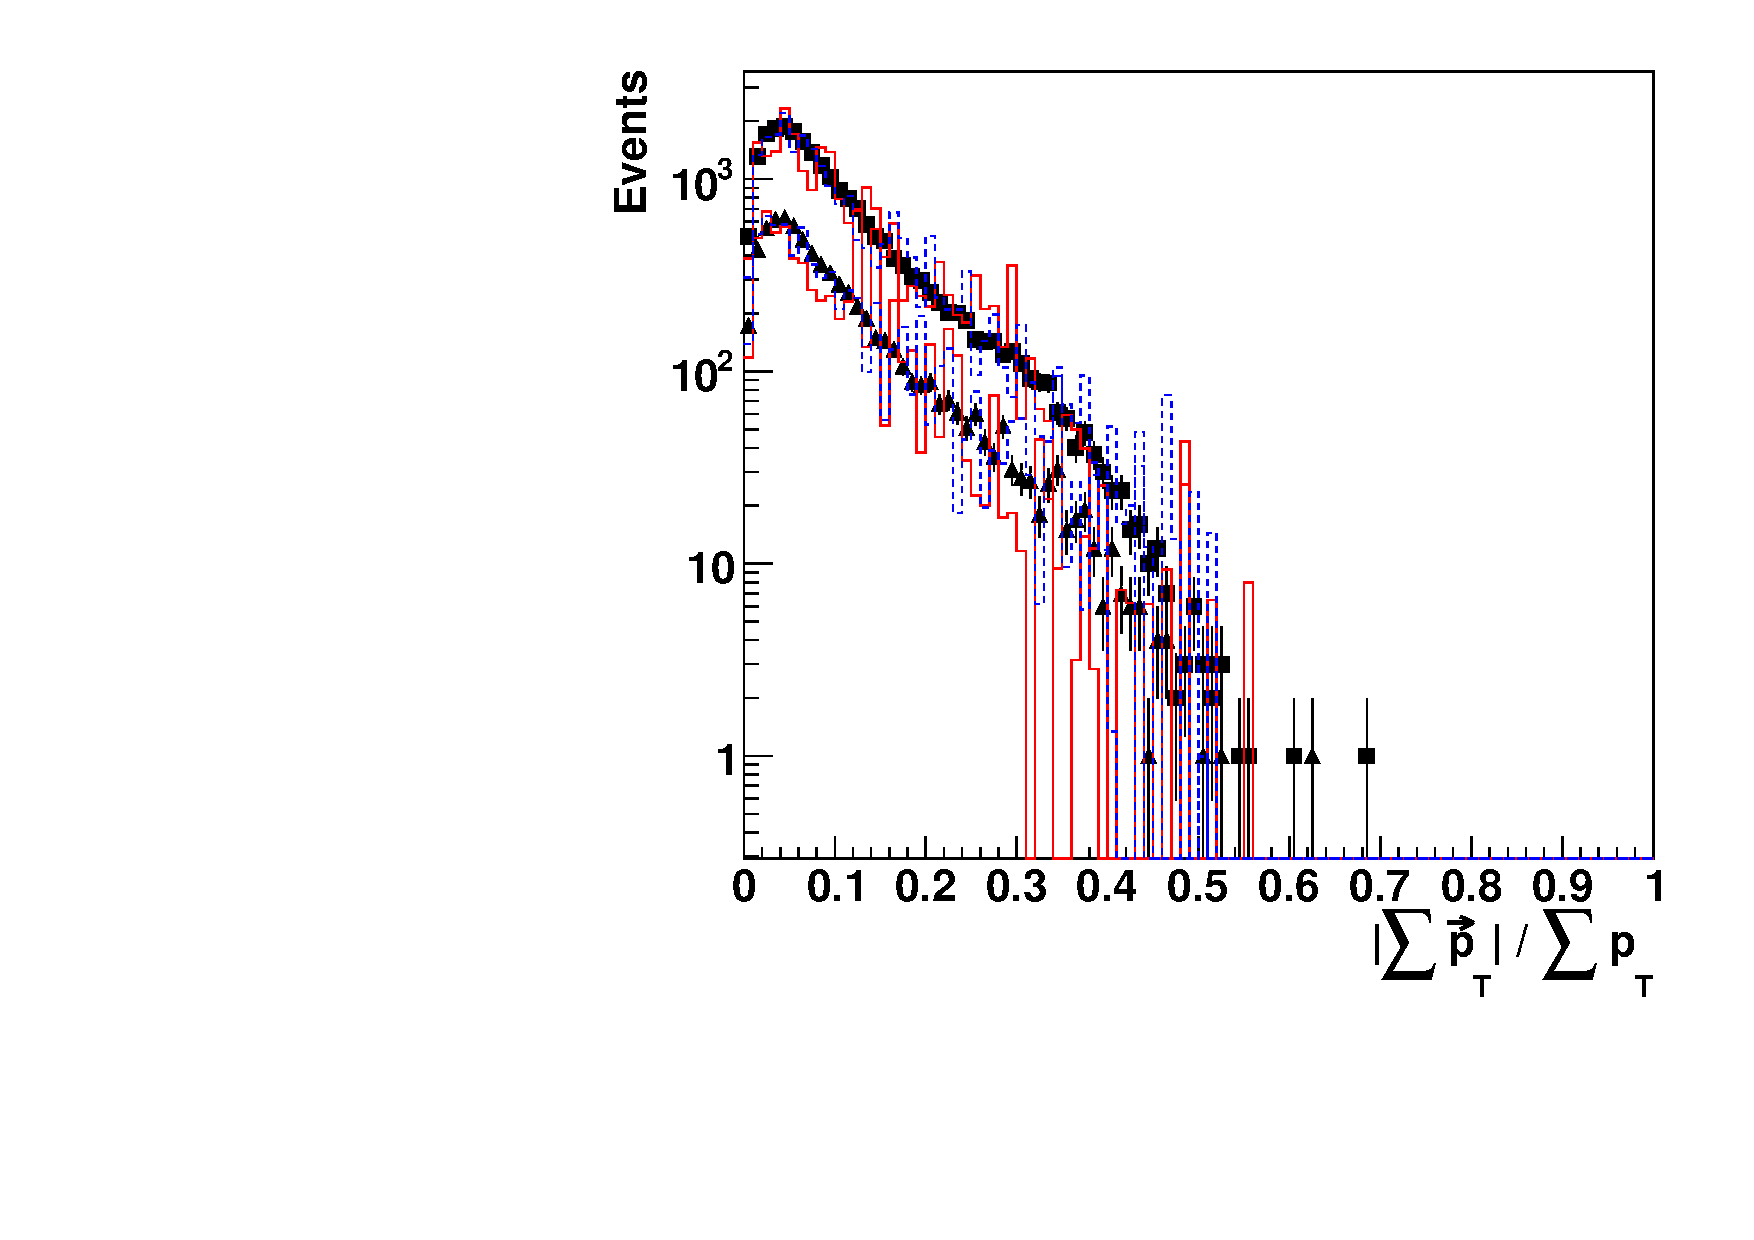
\includegraphics{figs/Data-MC-comparisons/PTVSPT-VVMiumHigh.pdf}} \\
%\end{tabular}
%  \caption[Delta Eta Double]{Comparisons between data and Monte Carlo
%                     for $|\sum{\vec{p}_{T}}| / \sum{p_{T}}$ of the two leading jets of low purity (left) and low-high purity (right) 2-tagged events. The MC is normalized to the number of data events in each category. }
%  \label{fig:metSumPtDouble}
%\end{figure}

\newpage
\begin{figure}[htb]
\centering
\begin{tabular}{cc}
     \resizebox{0.5\linewidth}{!}{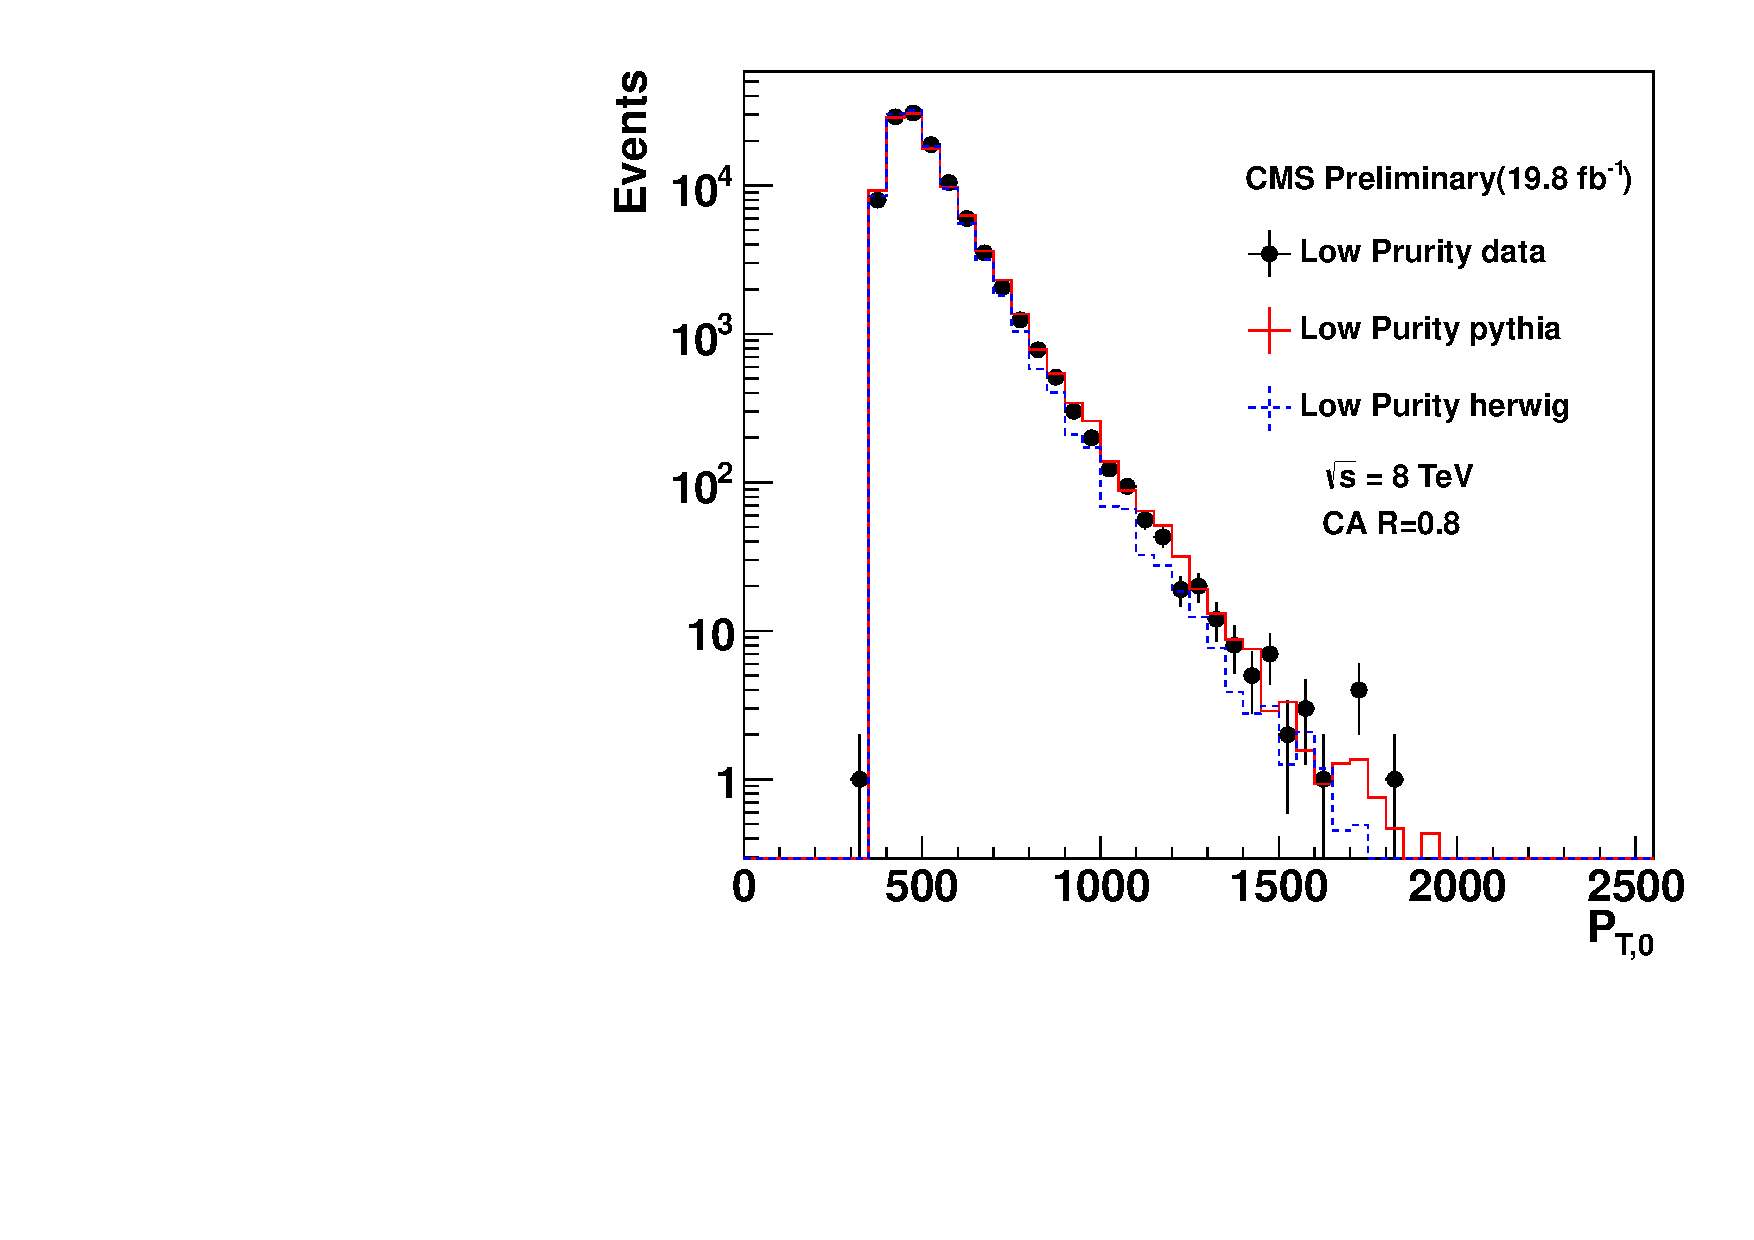
\includegraphics{figs/Data-MC-comparisons/PT0-qVLowP.pdf}} &
     \resizebox{0.5\linewidth}{!}{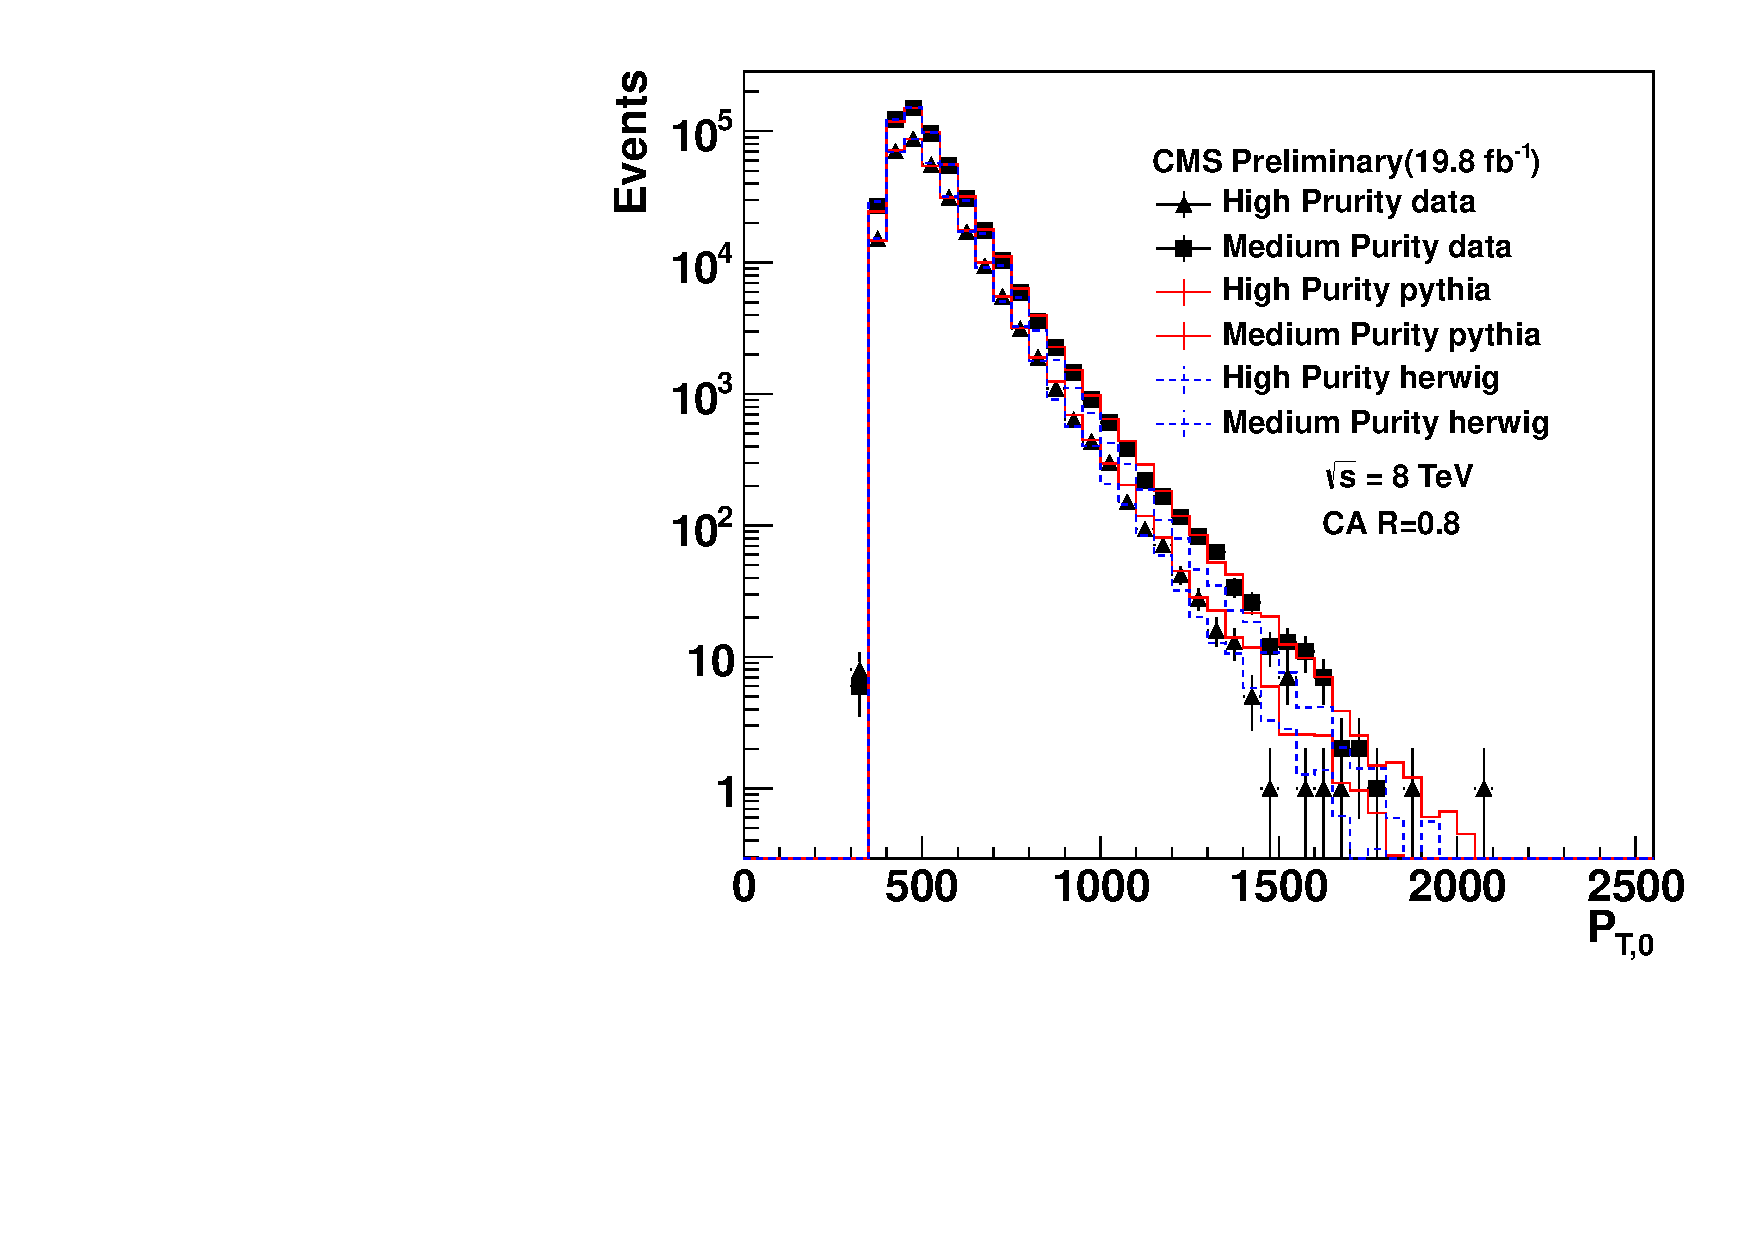
\includegraphics{figs/Data-MC-comparisons/PT0-qVMiumHigh.pdf}} \\
\end{tabular}
  \caption[PT Single]{Comparisons between data and Monte Carlo
                    for $\pt$ of the leading jet of low purity (left) and low-high purity (right) 1-tagged events.
	   The MC is normalized to the number of data events in each category. }
  \label{fig:Pt0Single}
\end{figure}

\begin{figure}[htb]
\centering
\begin{tabular}{cc}
     \resizebox{0.5\linewidth}{!}{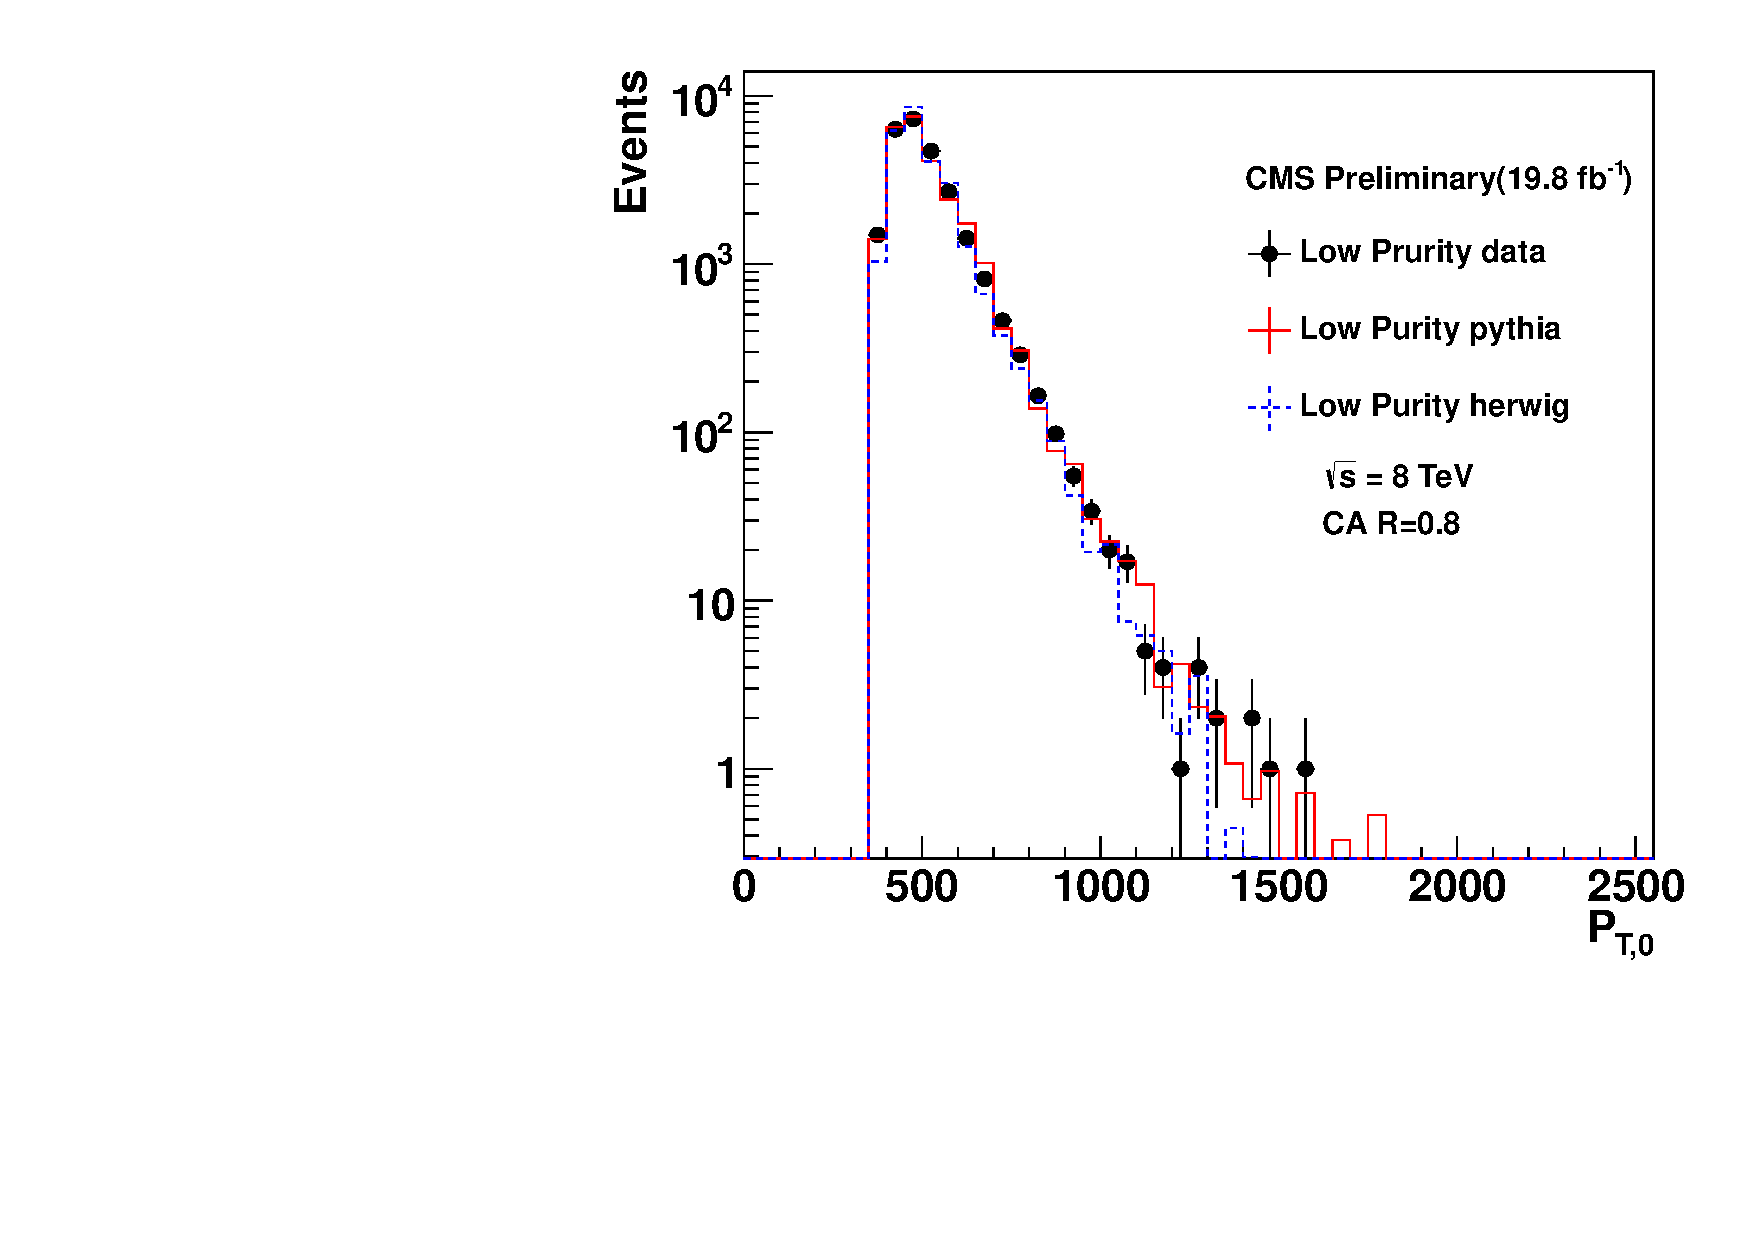
\includegraphics{figs/Data-MC-comparisons/PT0-VVLowP.pdf}} &
     \resizebox{0.5\linewidth}{!}{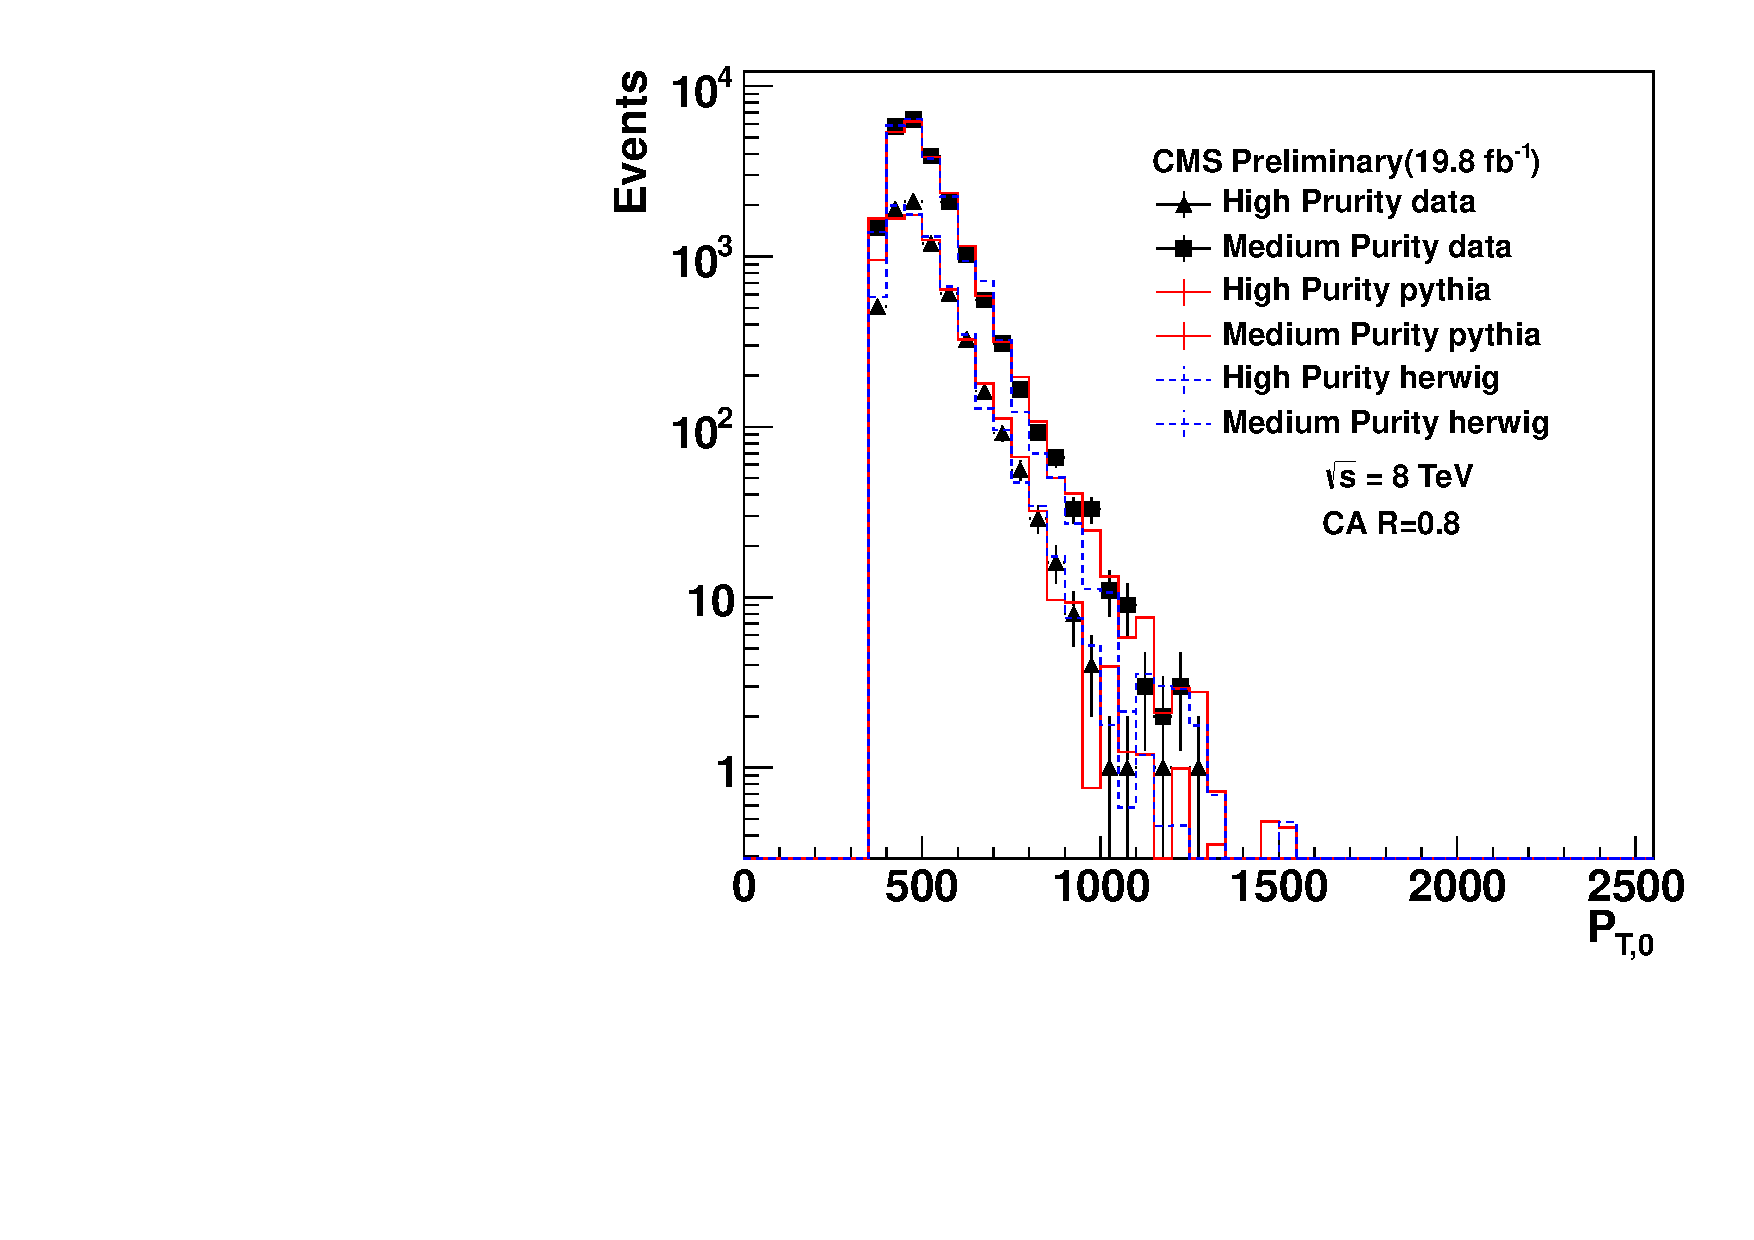
\includegraphics{figs/Data-MC-comparisons/PT0-VVMiumHigh.pdf}} \\
\end{tabular}
  \caption[Delta Eta Double]{Comparisons between data and Monte Carlo
                     for $\pt$ of the leading jet of low purity (left) and low-high purity (right) 2-tagged events. The MC is normalized to the number of data events in each category. }
  \label{fig:Pt0Double}
\end{figure}

\newpage
\begin{figure}[htb]
\centering
\begin{tabular}{cc}
     \resizebox{0.5\linewidth}{!}{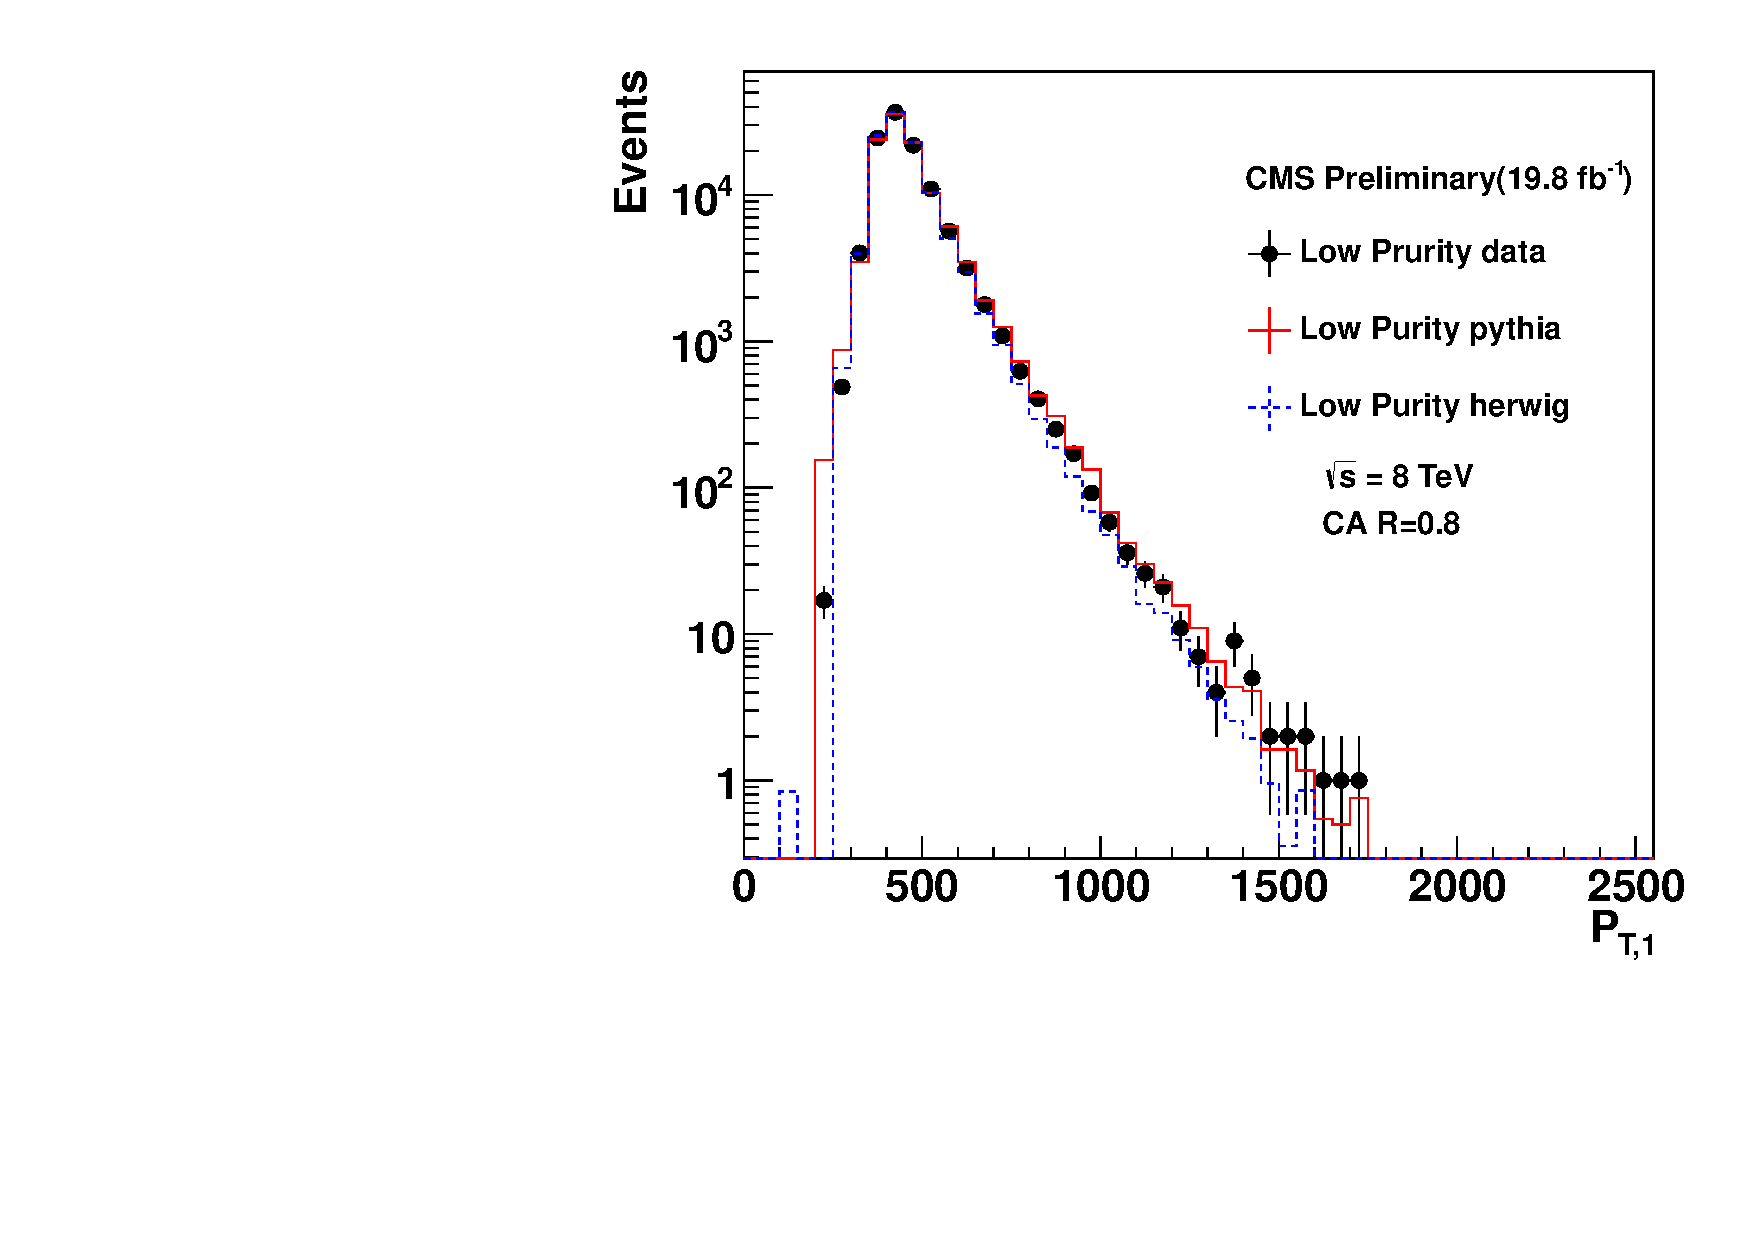
\includegraphics{figs/Data-MC-comparisons/PT1-qVLowP.pdf}} &
     \resizebox{0.5\linewidth}{!}{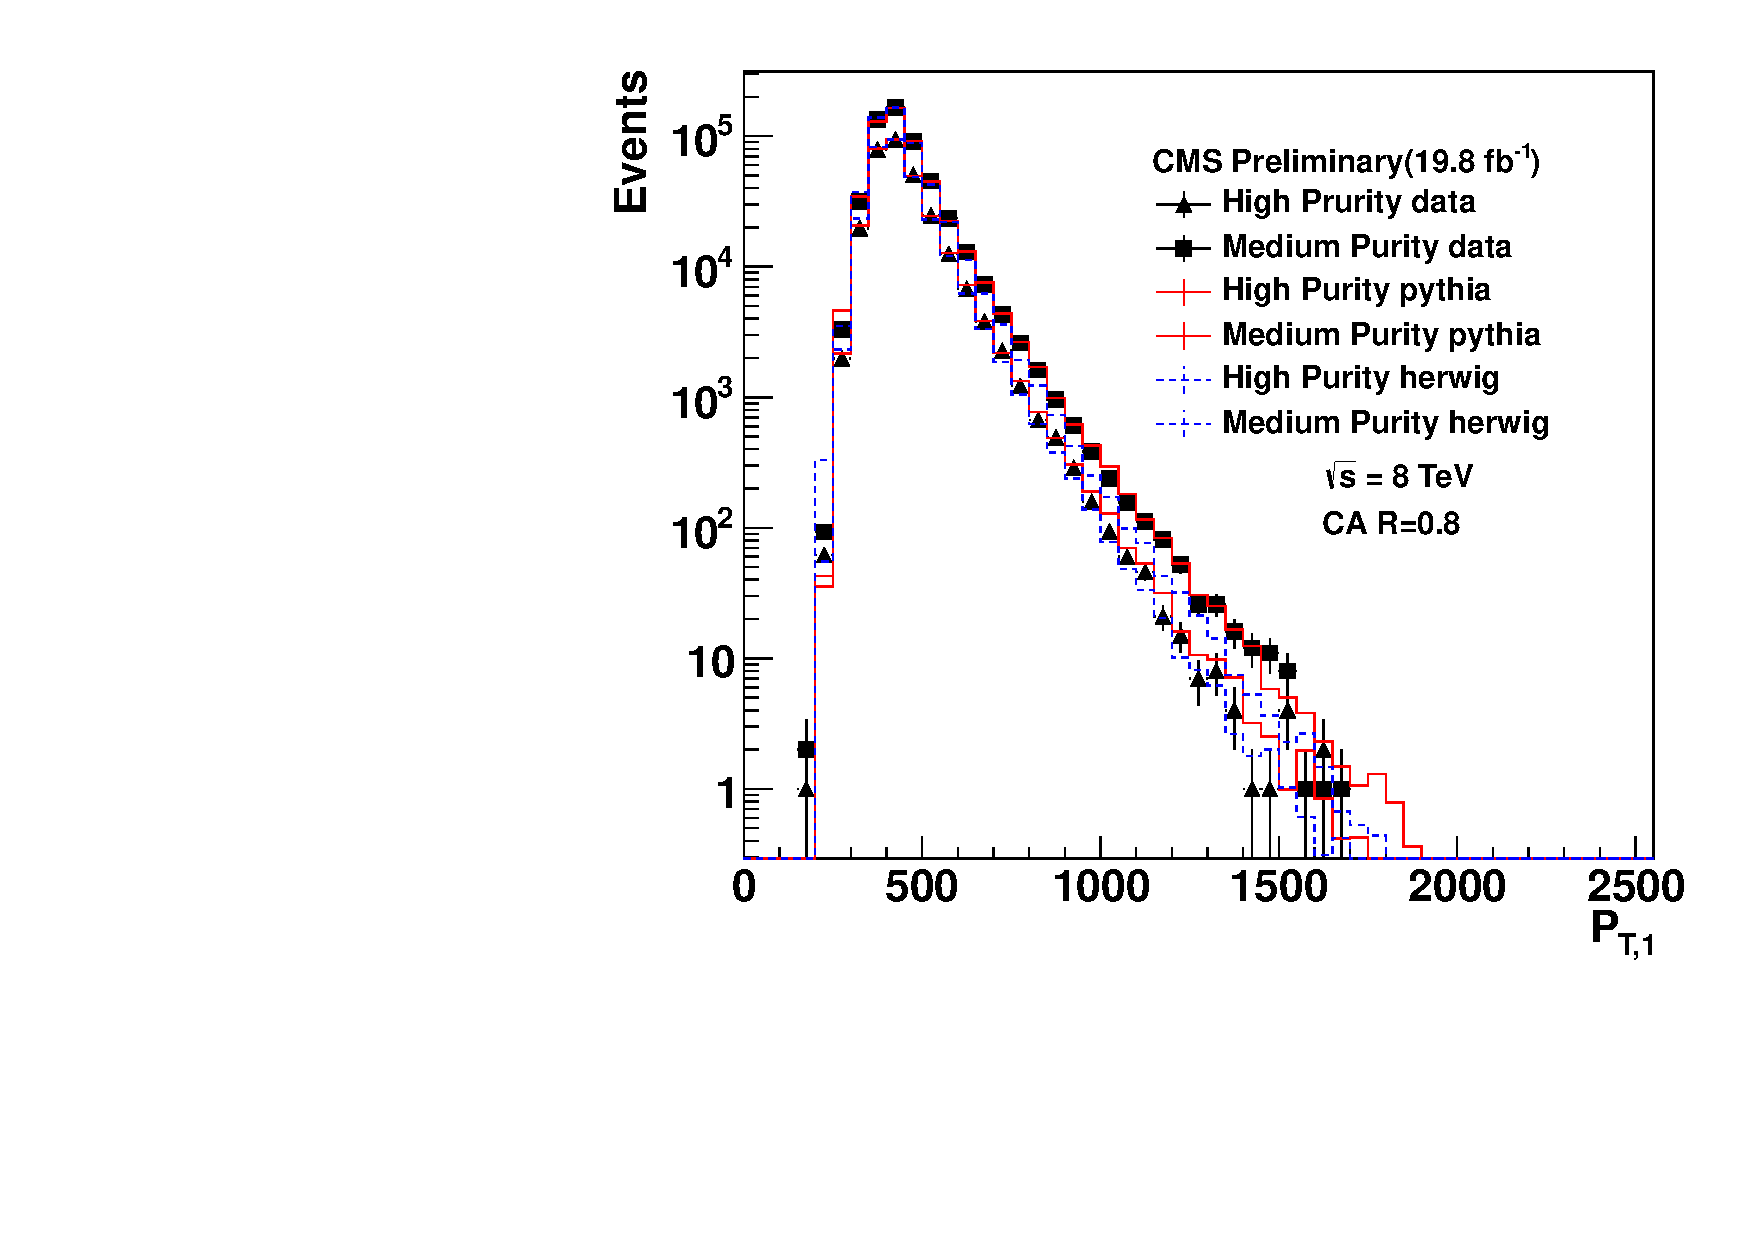
\includegraphics{figs/Data-MC-comparisons/PT1-qVMiumHigh.pdf}} \\
\end{tabular}
  \caption[PT Single]{Comparisons between data and Monte Carlo
                    for $\pt$ of the second leading jet of low purity (left) and low-high purity (right) 1-tagged events.
	   The MC is normalized to the number of data events in each category. }
  \label{fig:Pt1Single}
\end{figure}

\begin{figure}[htb]
\centering
\begin{tabular}{cc}
     \resizebox{0.5\linewidth}{!}{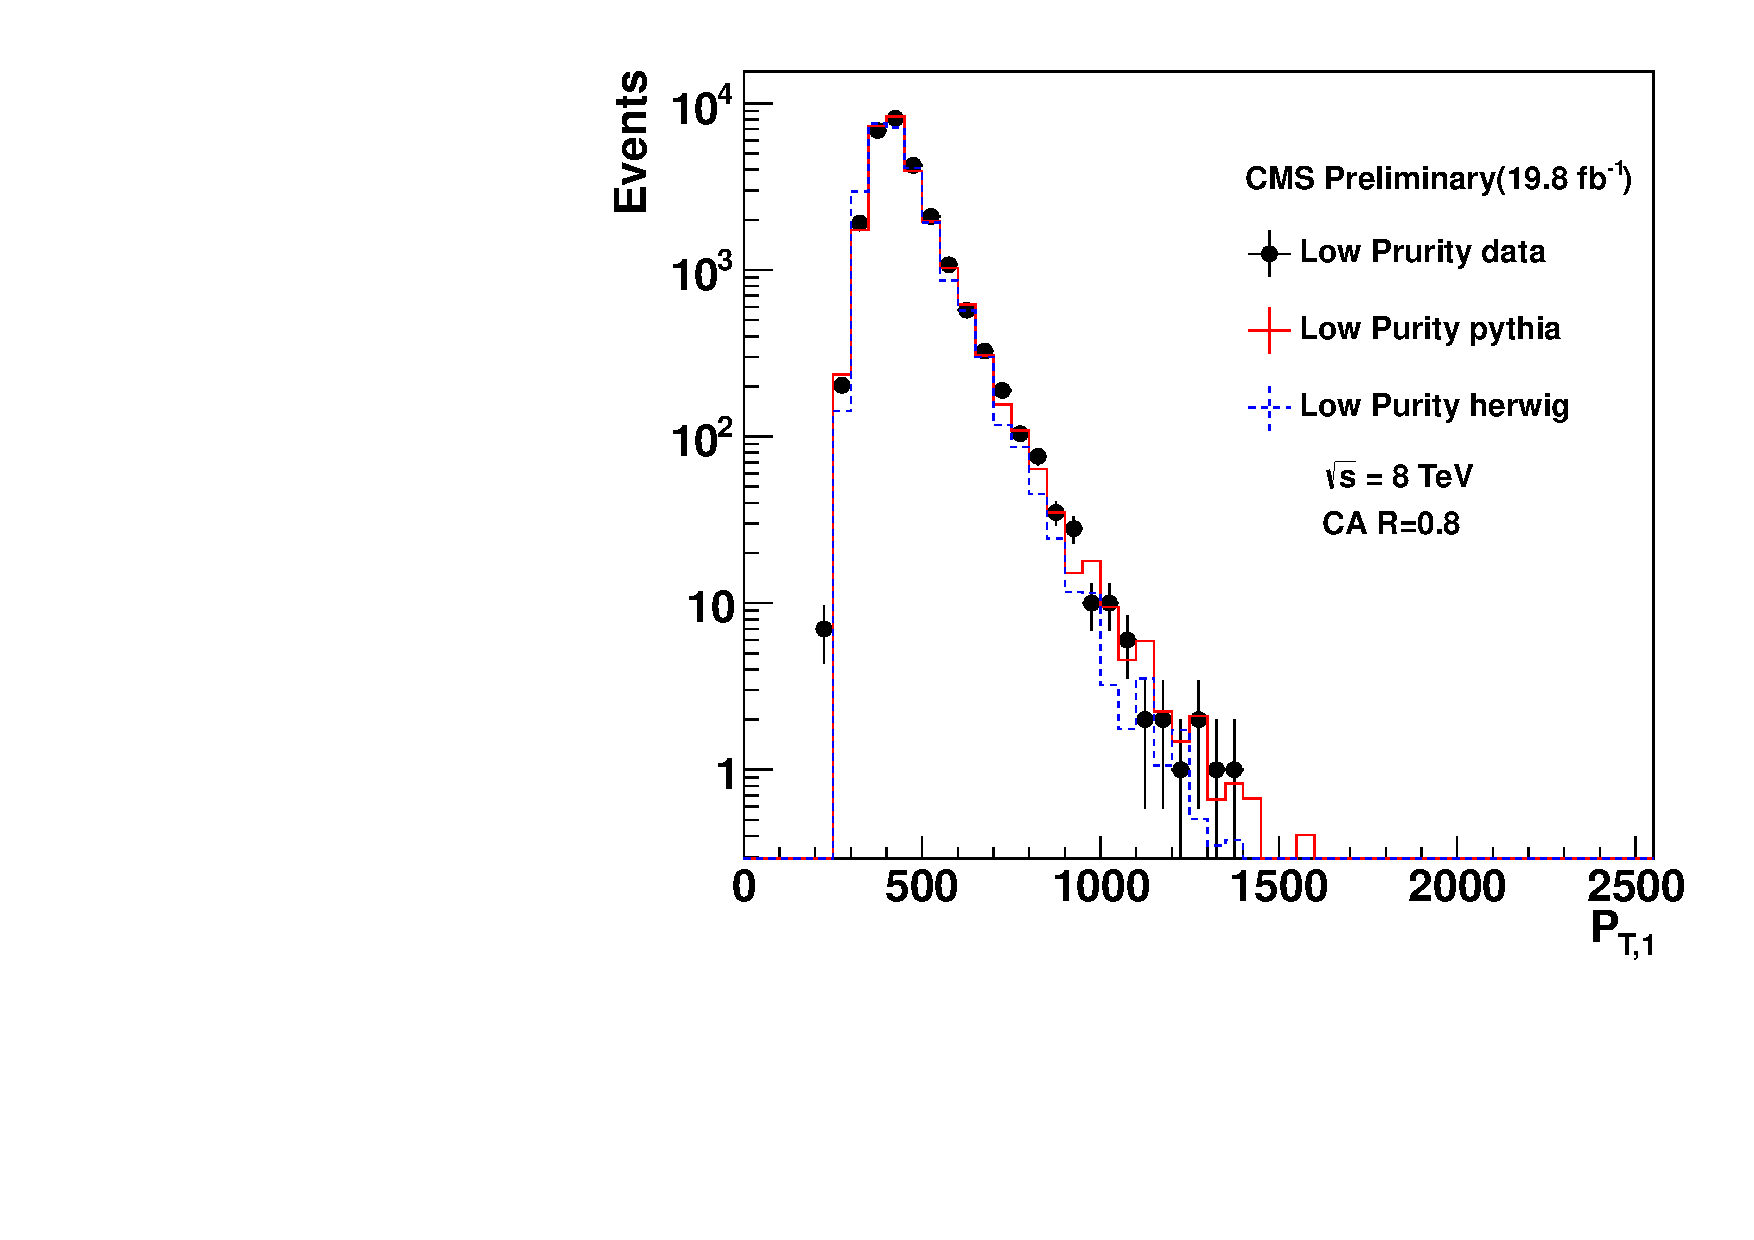
\includegraphics{figs/Data-MC-comparisons/PT1-VVLowP.pdf}} &
     \resizebox{0.5\linewidth}{!}{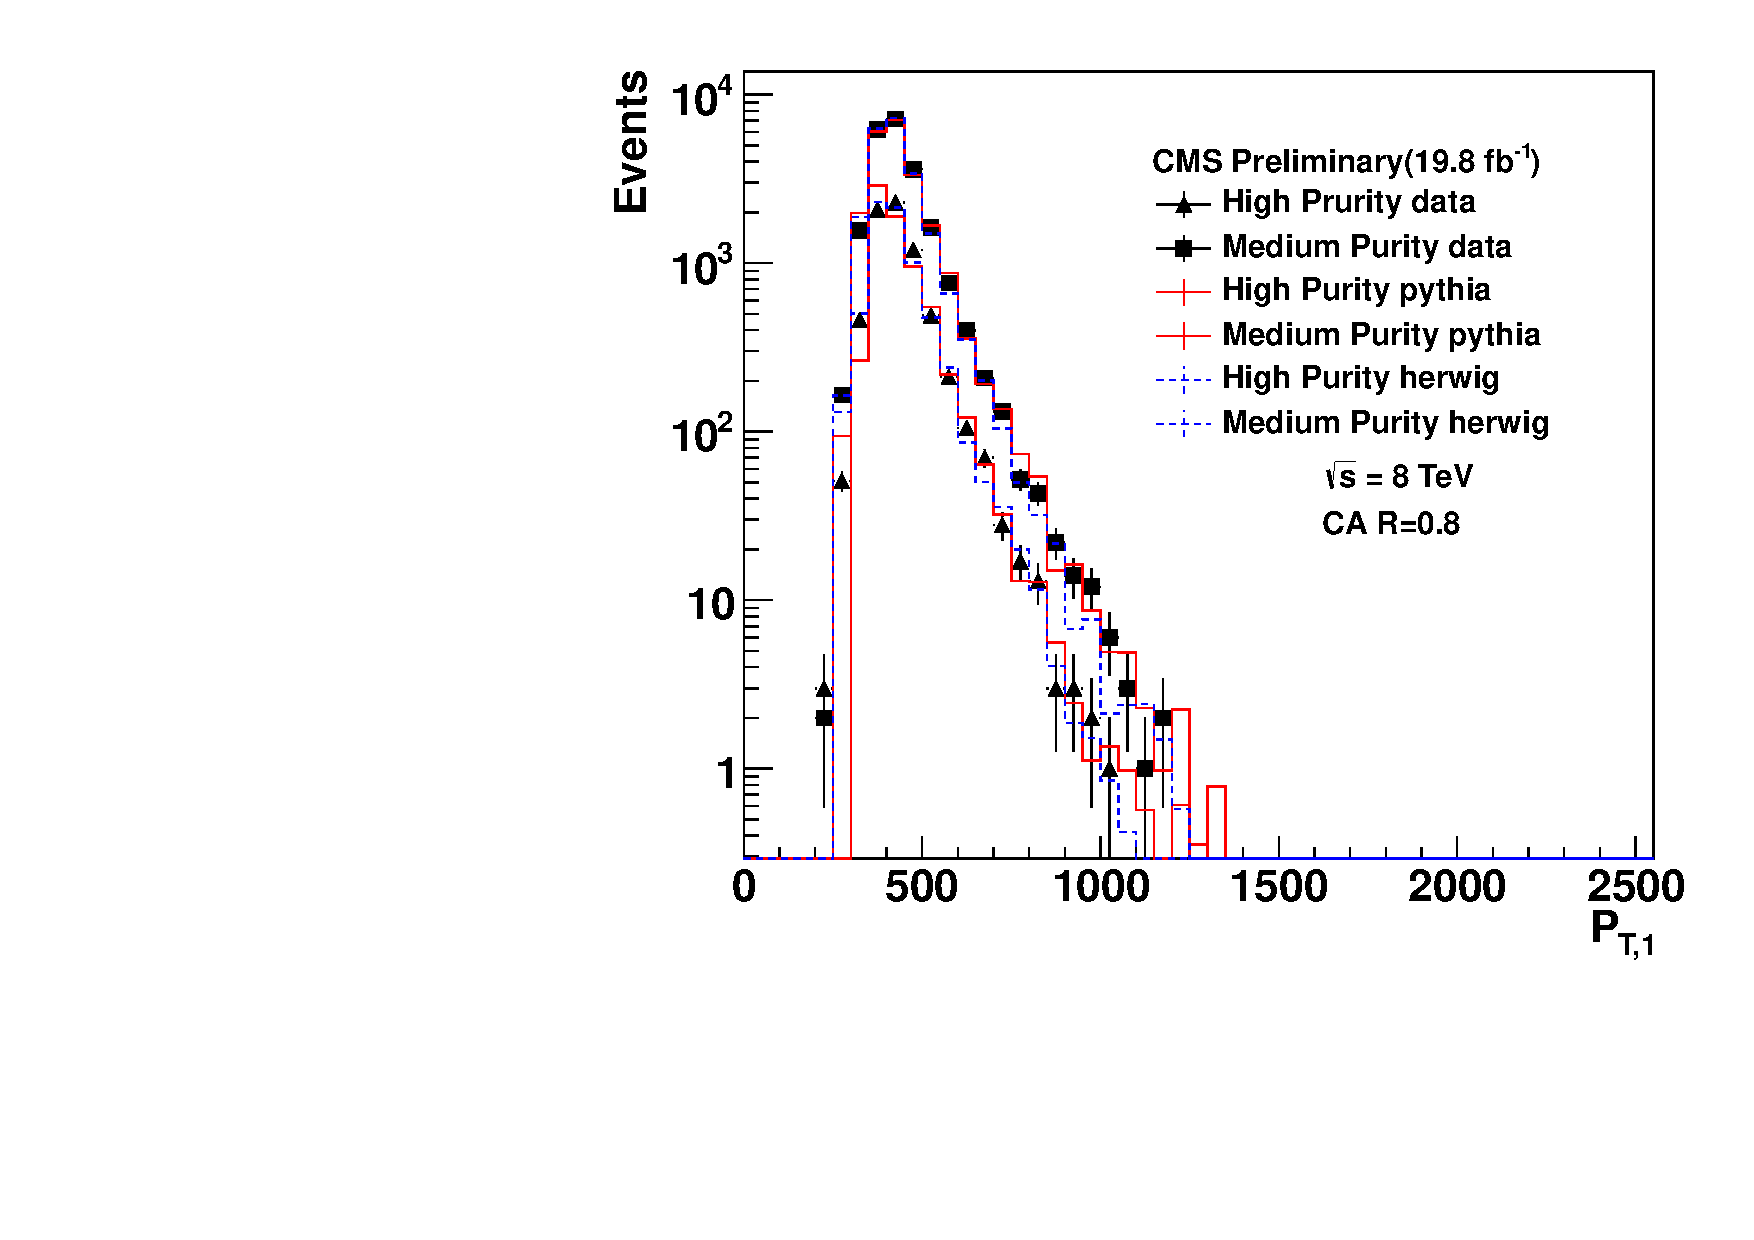
\includegraphics{figs/Data-MC-comparisons/PT1-VVMiumHigh.pdf}} \\
\end{tabular}
  \caption[Delta Eta Double]{Comparisons between data and Monte Carlo
                     for $\pt$ of the second leading jet of low purity (left) and low-high purity (right) 2-tagged events. The MC is normalized to the number of data events in each category. }
  \label{fig:Pt1Double}
\end{figure}



\newpage
\begin{figure}[htb]
\centering
\begin{tabular}{cc}
     \resizebox{0.5\linewidth}{!}{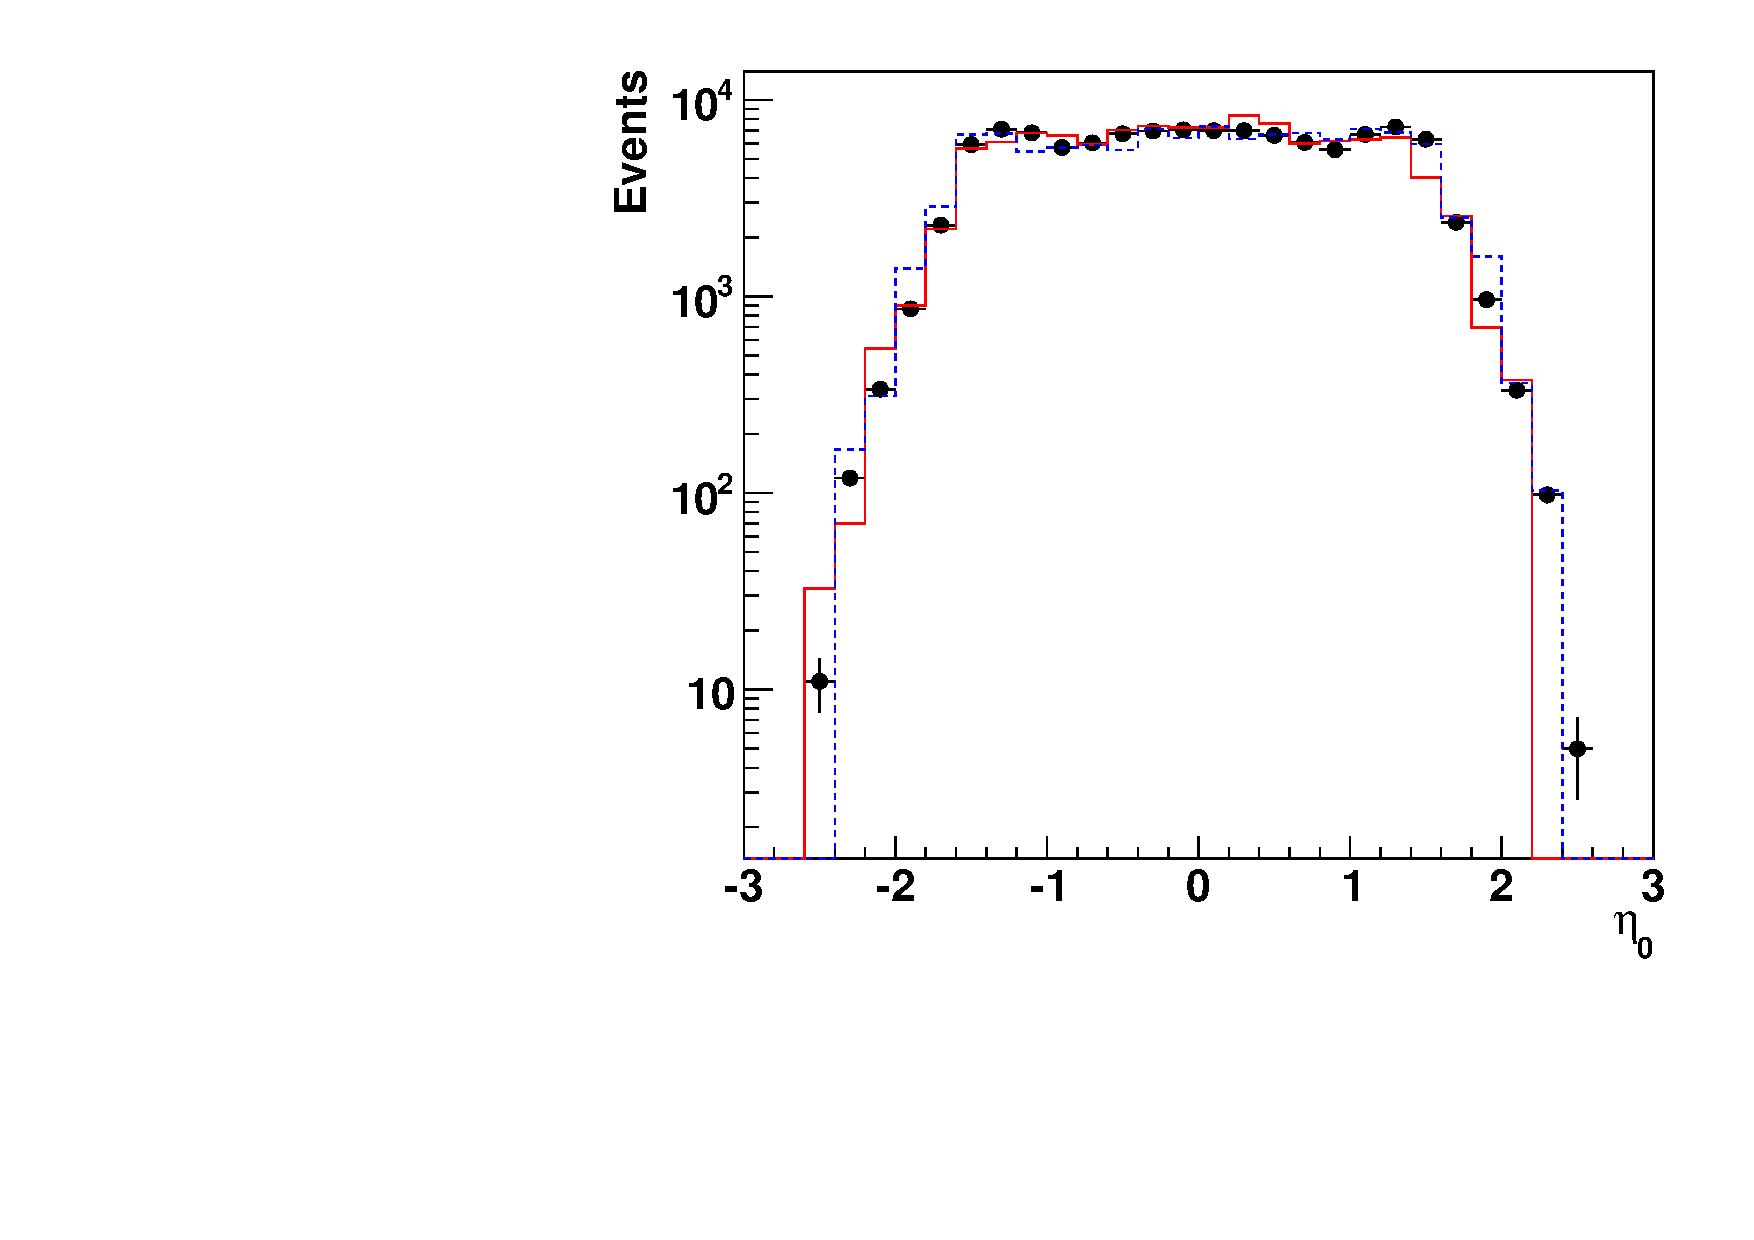
\includegraphics{figs/Data-MC-comparisons/Eta0-qVLowP.pdf}} &
     \resizebox{0.5\linewidth}{!}{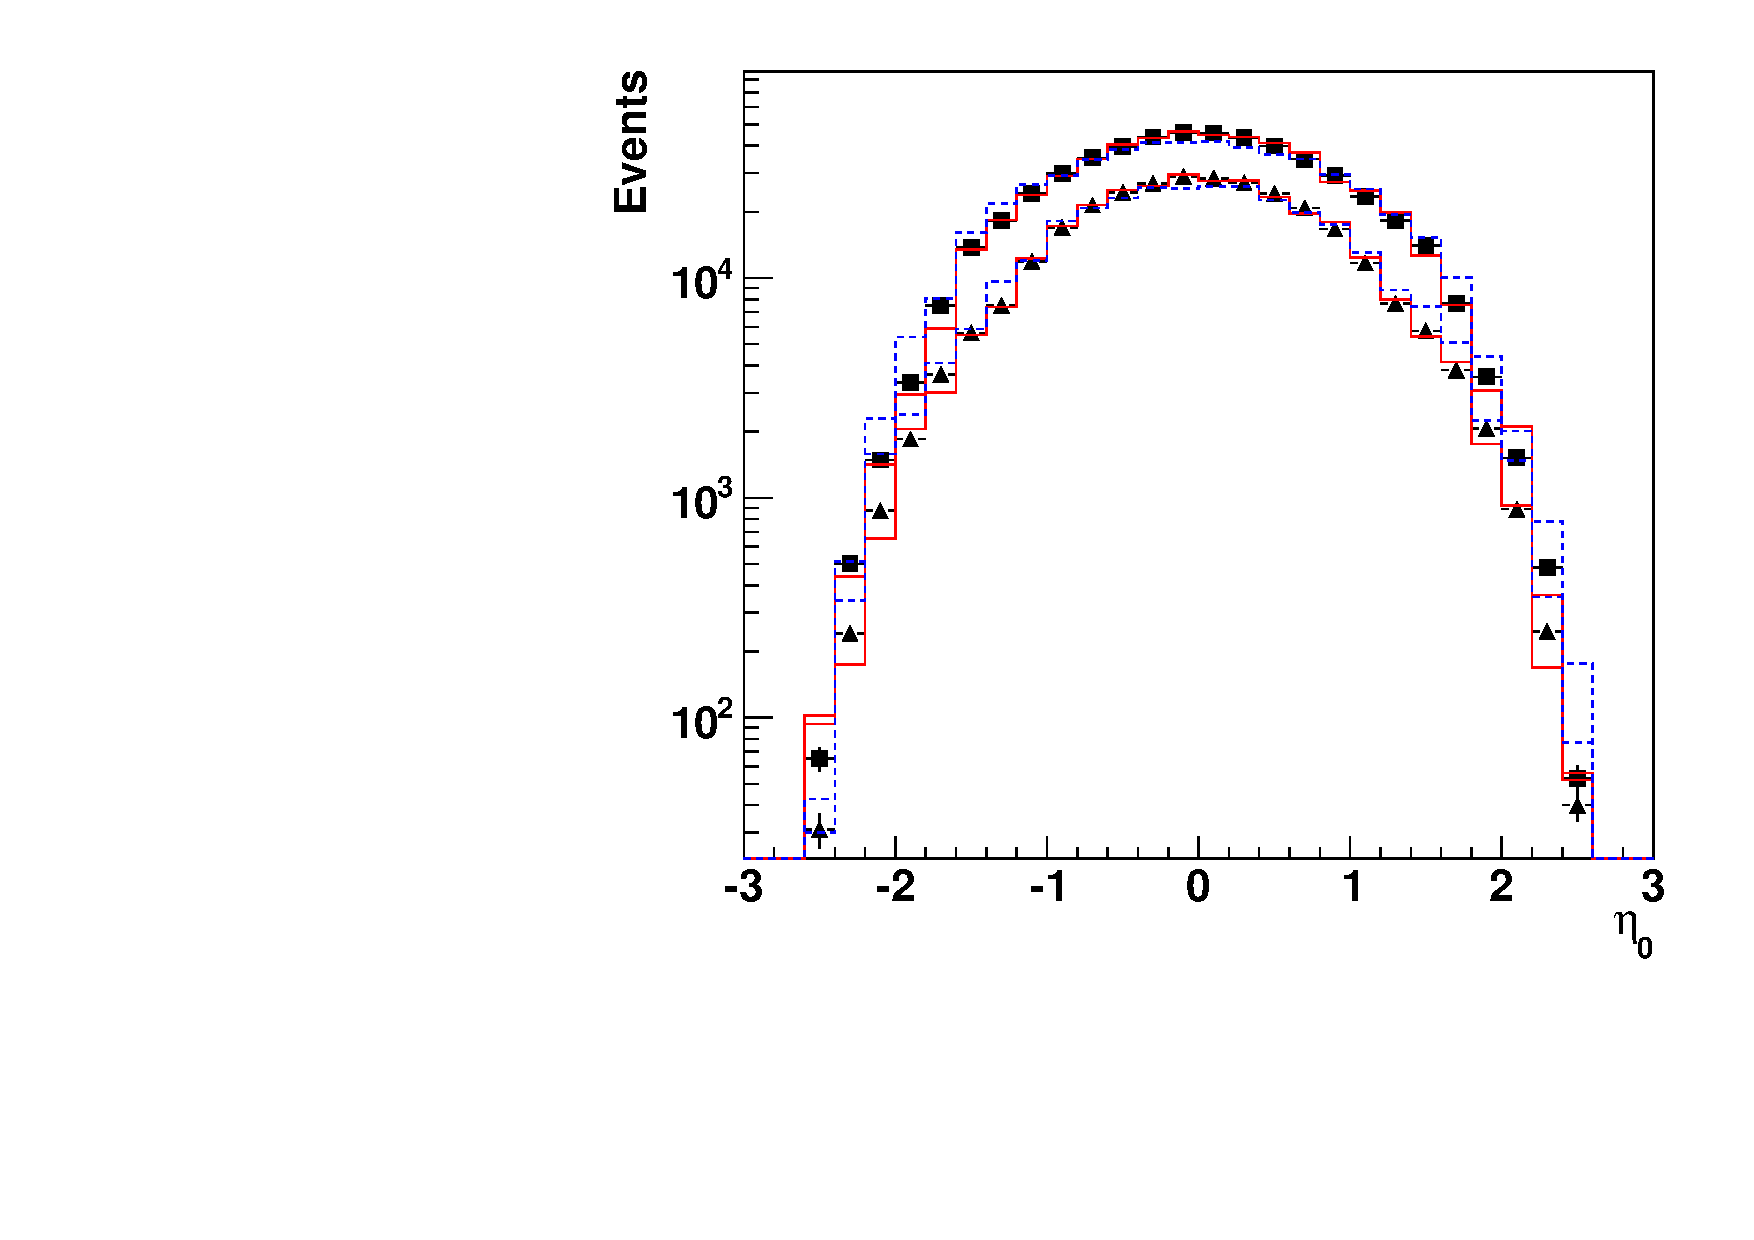
\includegraphics{figs/Data-MC-comparisons/Eta0-qVMiumHigh.pdf}} \\
\end{tabular}
  \caption[PT Single]{Comparisons between data and Monte Carlo
                    for $\eta$ of the leading jet of low purity (left) and low-high purity (right) 1-tagged events.
	   The MC is normalized to the number of data events in each category. }
  \label{fig:Eta0Single}
\end{figure}

\begin{figure}[htb]
\centering
\begin{tabular}{cc}
     \resizebox{0.5\linewidth}{!}{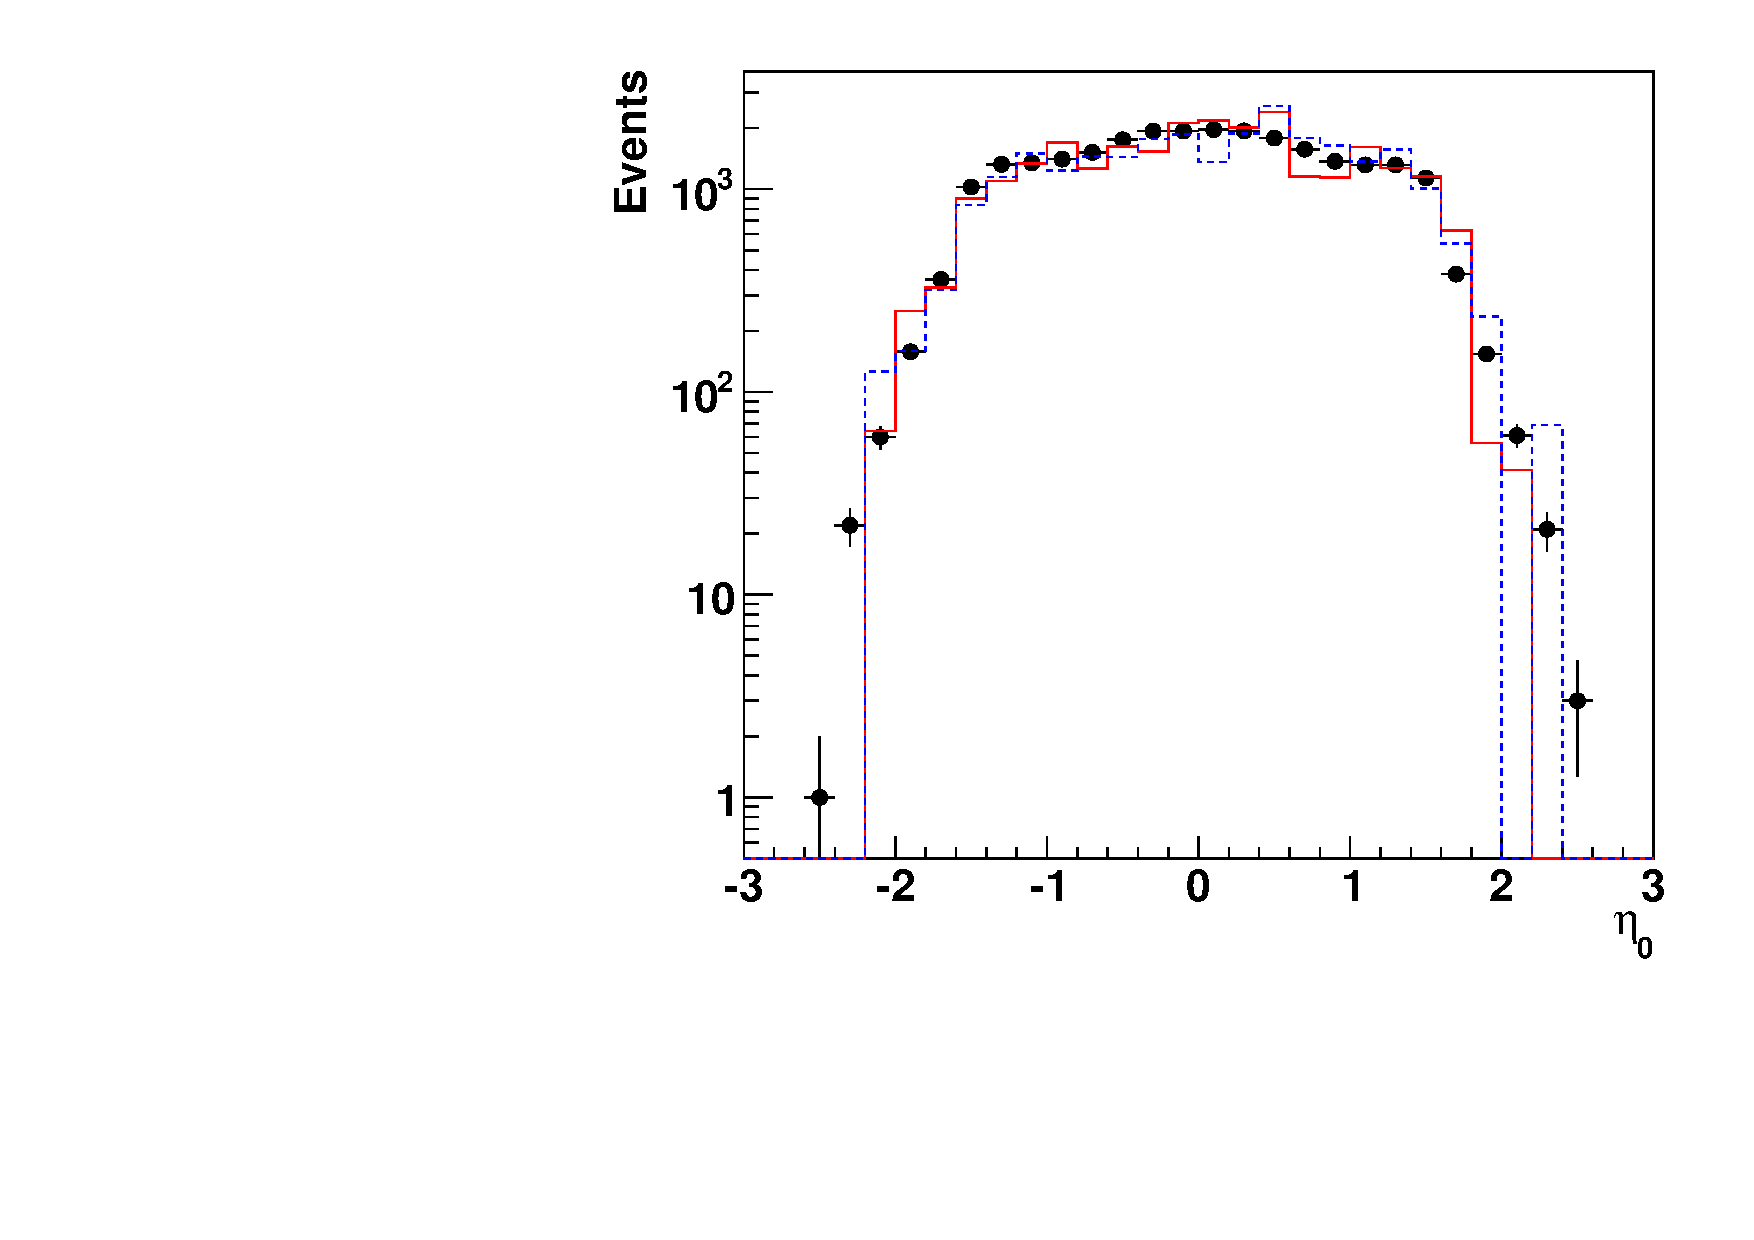
\includegraphics{figs/Data-MC-comparisons/Eta0-VVLowP.pdf}} &
     \resizebox{0.5\linewidth}{!}{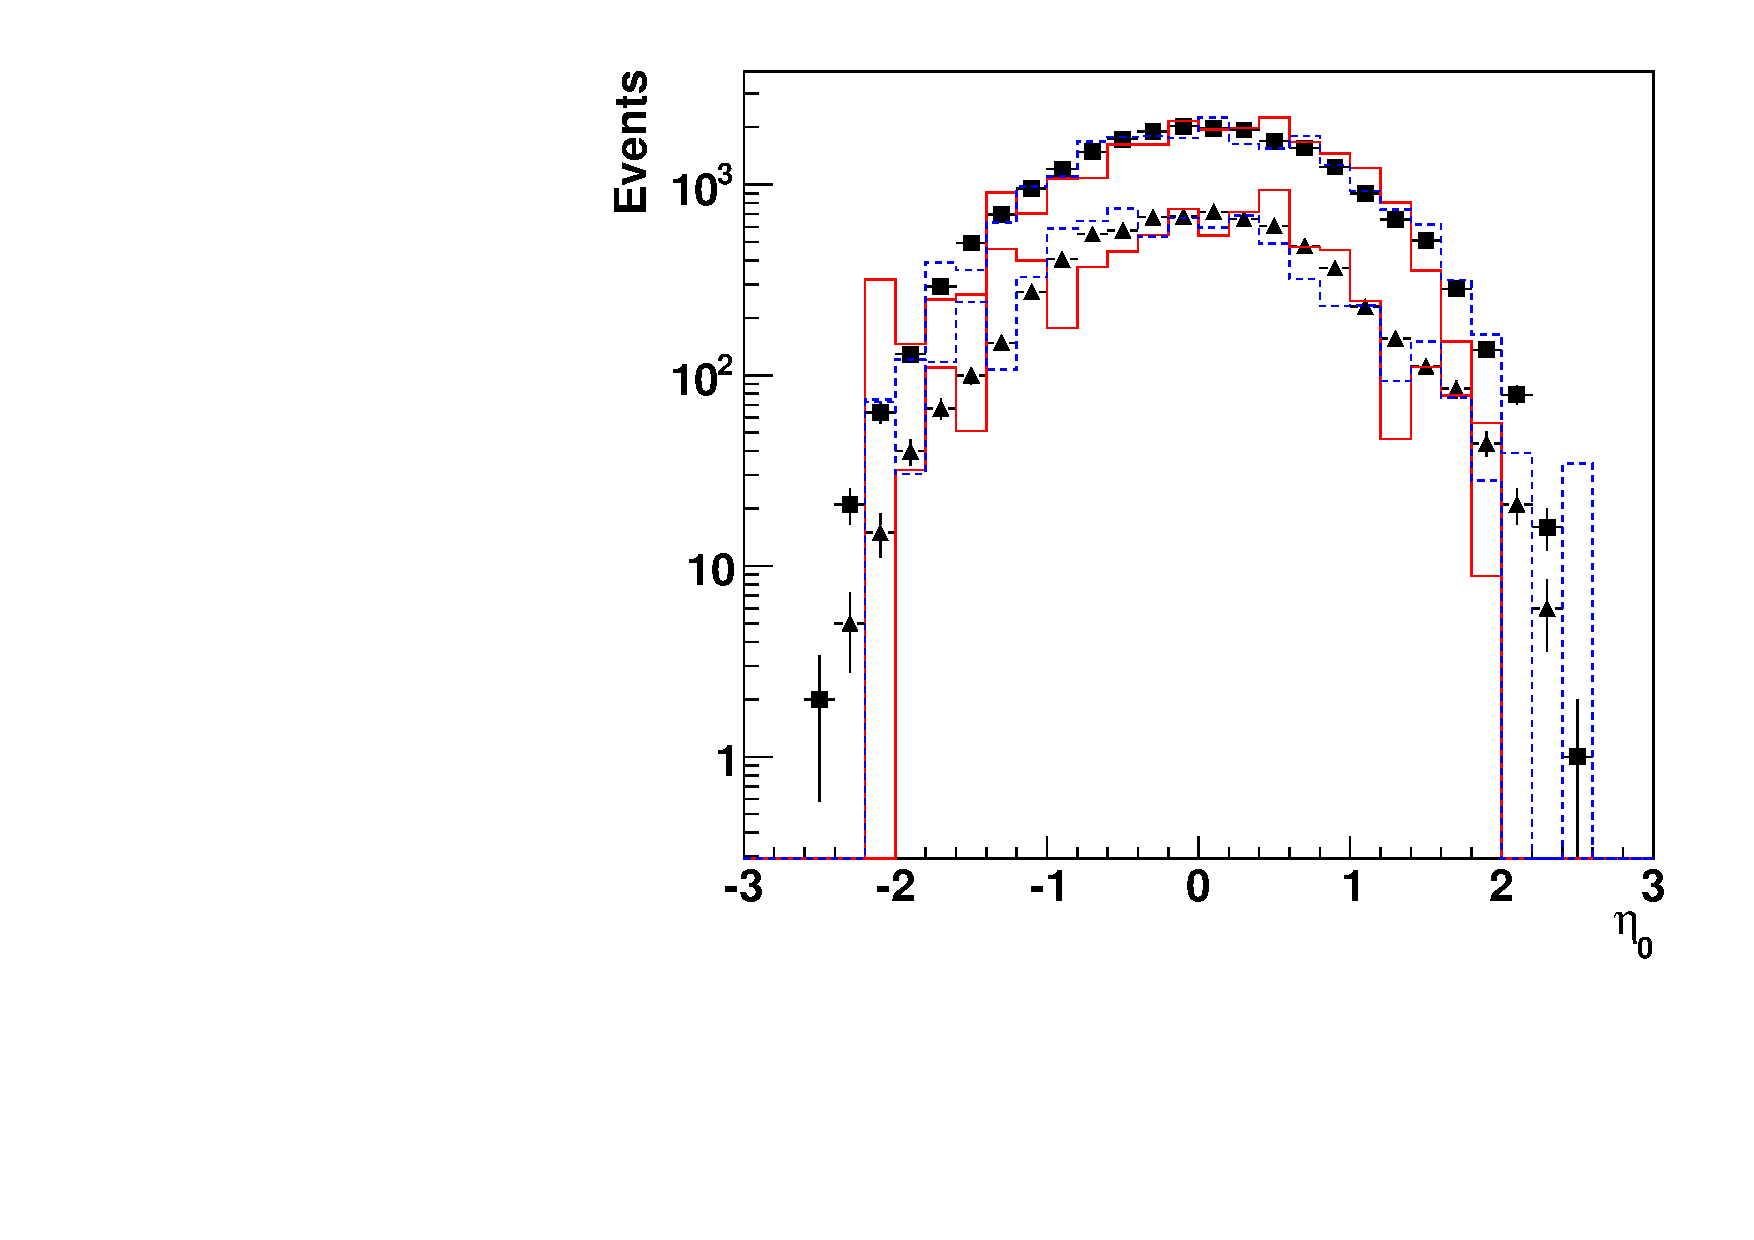
\includegraphics{figs/Data-MC-comparisons/Eta0-VVMiumHigh.pdf}} \\
\end{tabular}
  \caption[Delta Eta Double]{Comparisons between data and Monte Carlo
                     for $\eta$ of the leading jet of low purity (left) and low-high purity (right) 2-tagged events. The MC is normalized to the number of data events in each category. }
  \label{fig:Eta0Double}
\end{figure}


\newpage
\begin{figure}[htb]
\centering
\begin{tabular}{cc}
     \resizebox{0.5\linewidth}{!}{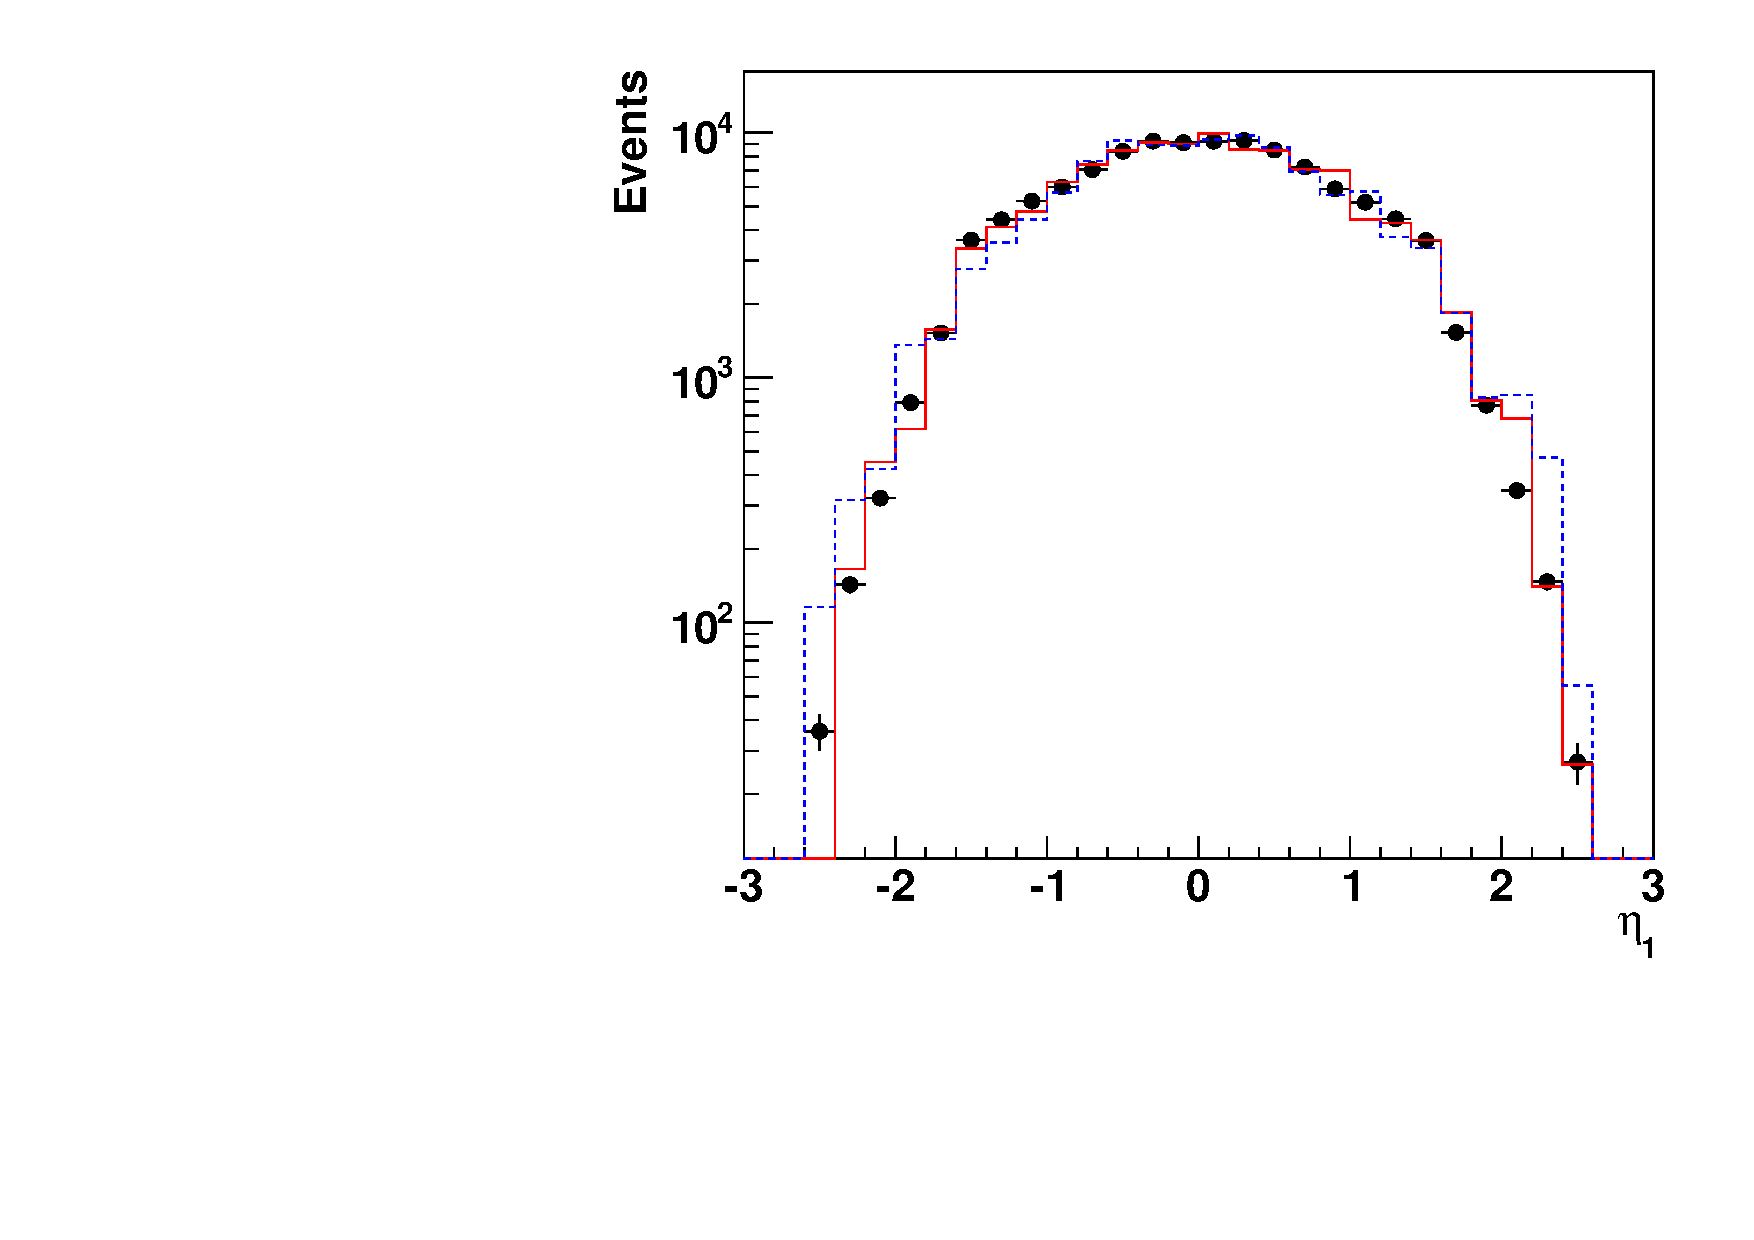
\includegraphics{figs/Data-MC-comparisons/Eta1-qVLowP.pdf}} &
     \resizebox{0.5\linewidth}{!}{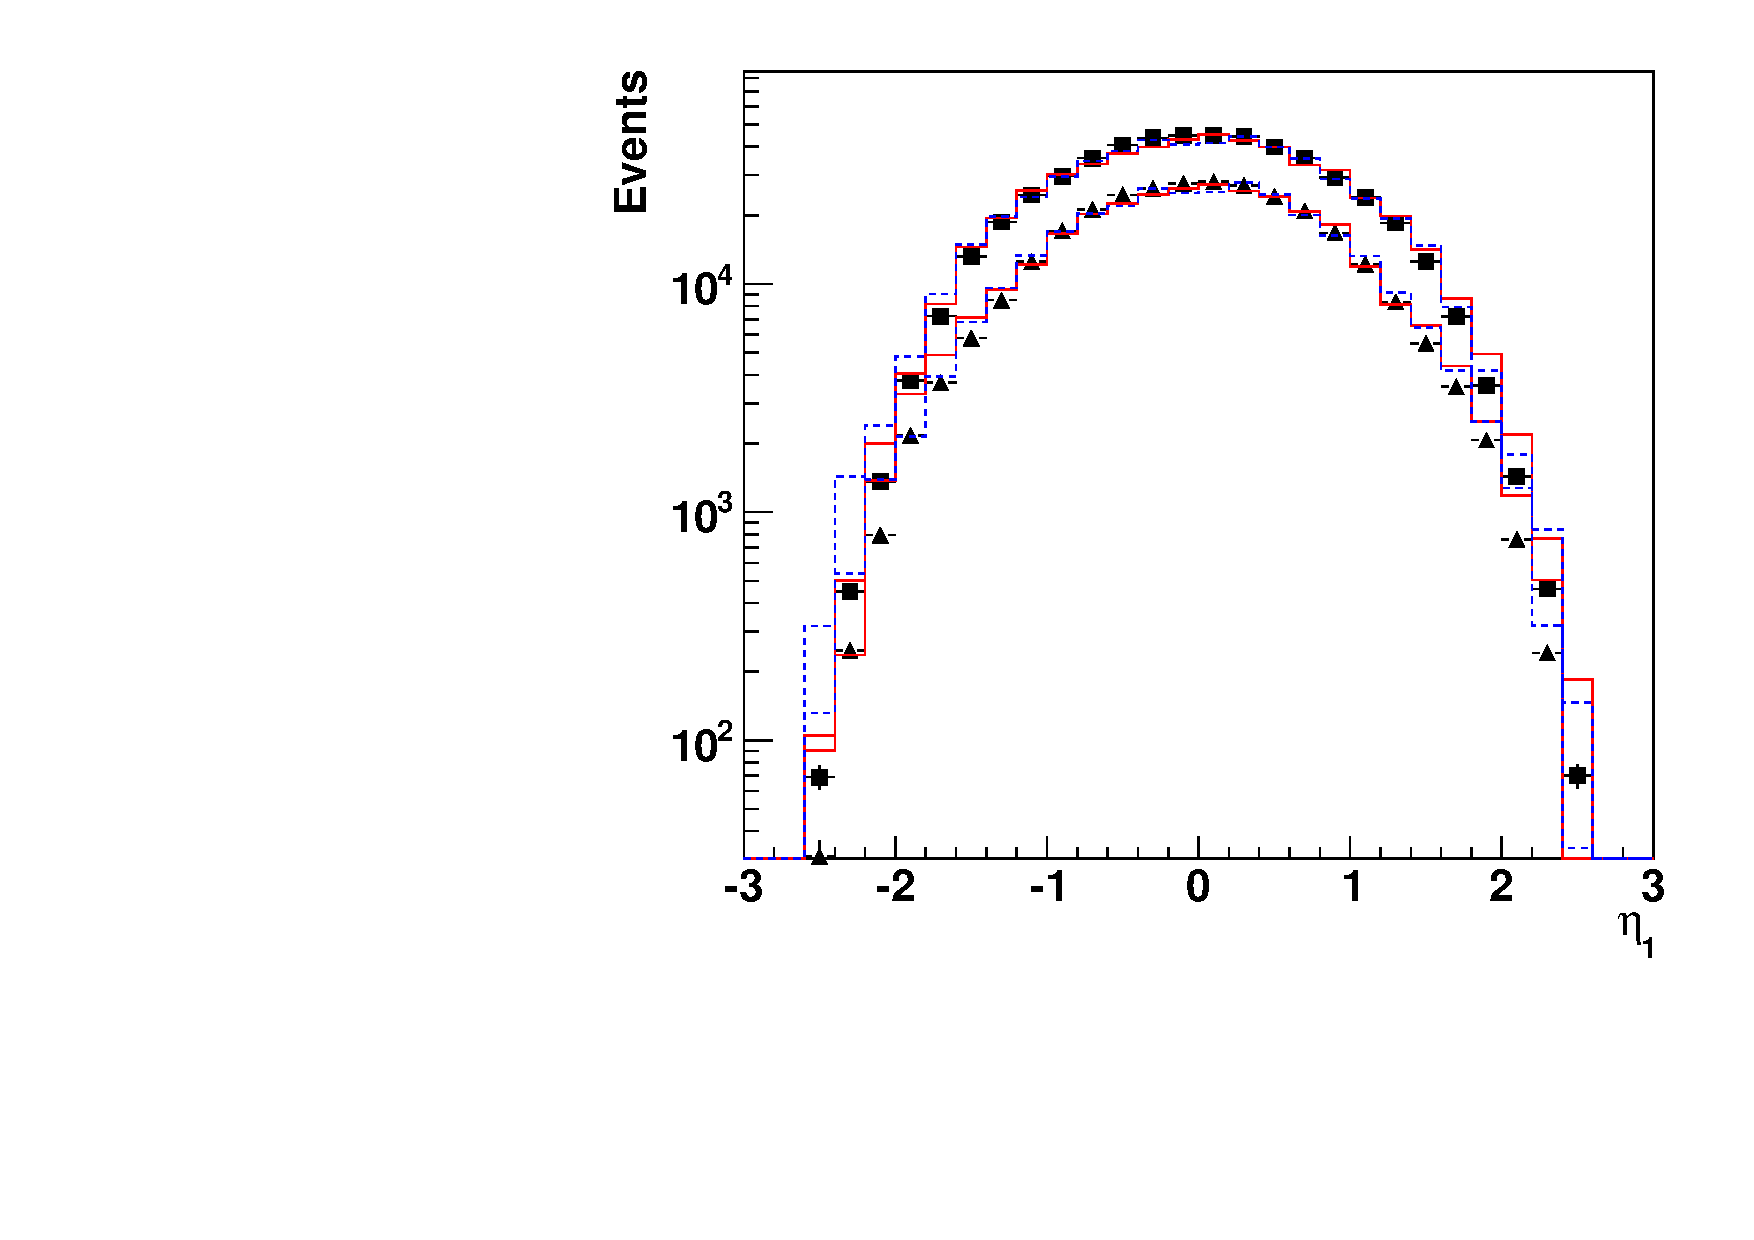
\includegraphics{figs/Data-MC-comparisons/Eta1-qVMiumHigh.pdf}} \\
\end{tabular}
  \caption[PT Single]{Comparisons between data and Monte Carlo
                    for $\eta$ of the second leading jet of low purity (left) and low-high purity (right) 1-tagged events.
	   The MC is normalized to the number of data events in each category. }
  \label{fig:Eta1Single}
\end{figure}

\begin{figure}[htb]
\centering
\begin{tabular}{cc}
     \resizebox{0.5\linewidth}{!}{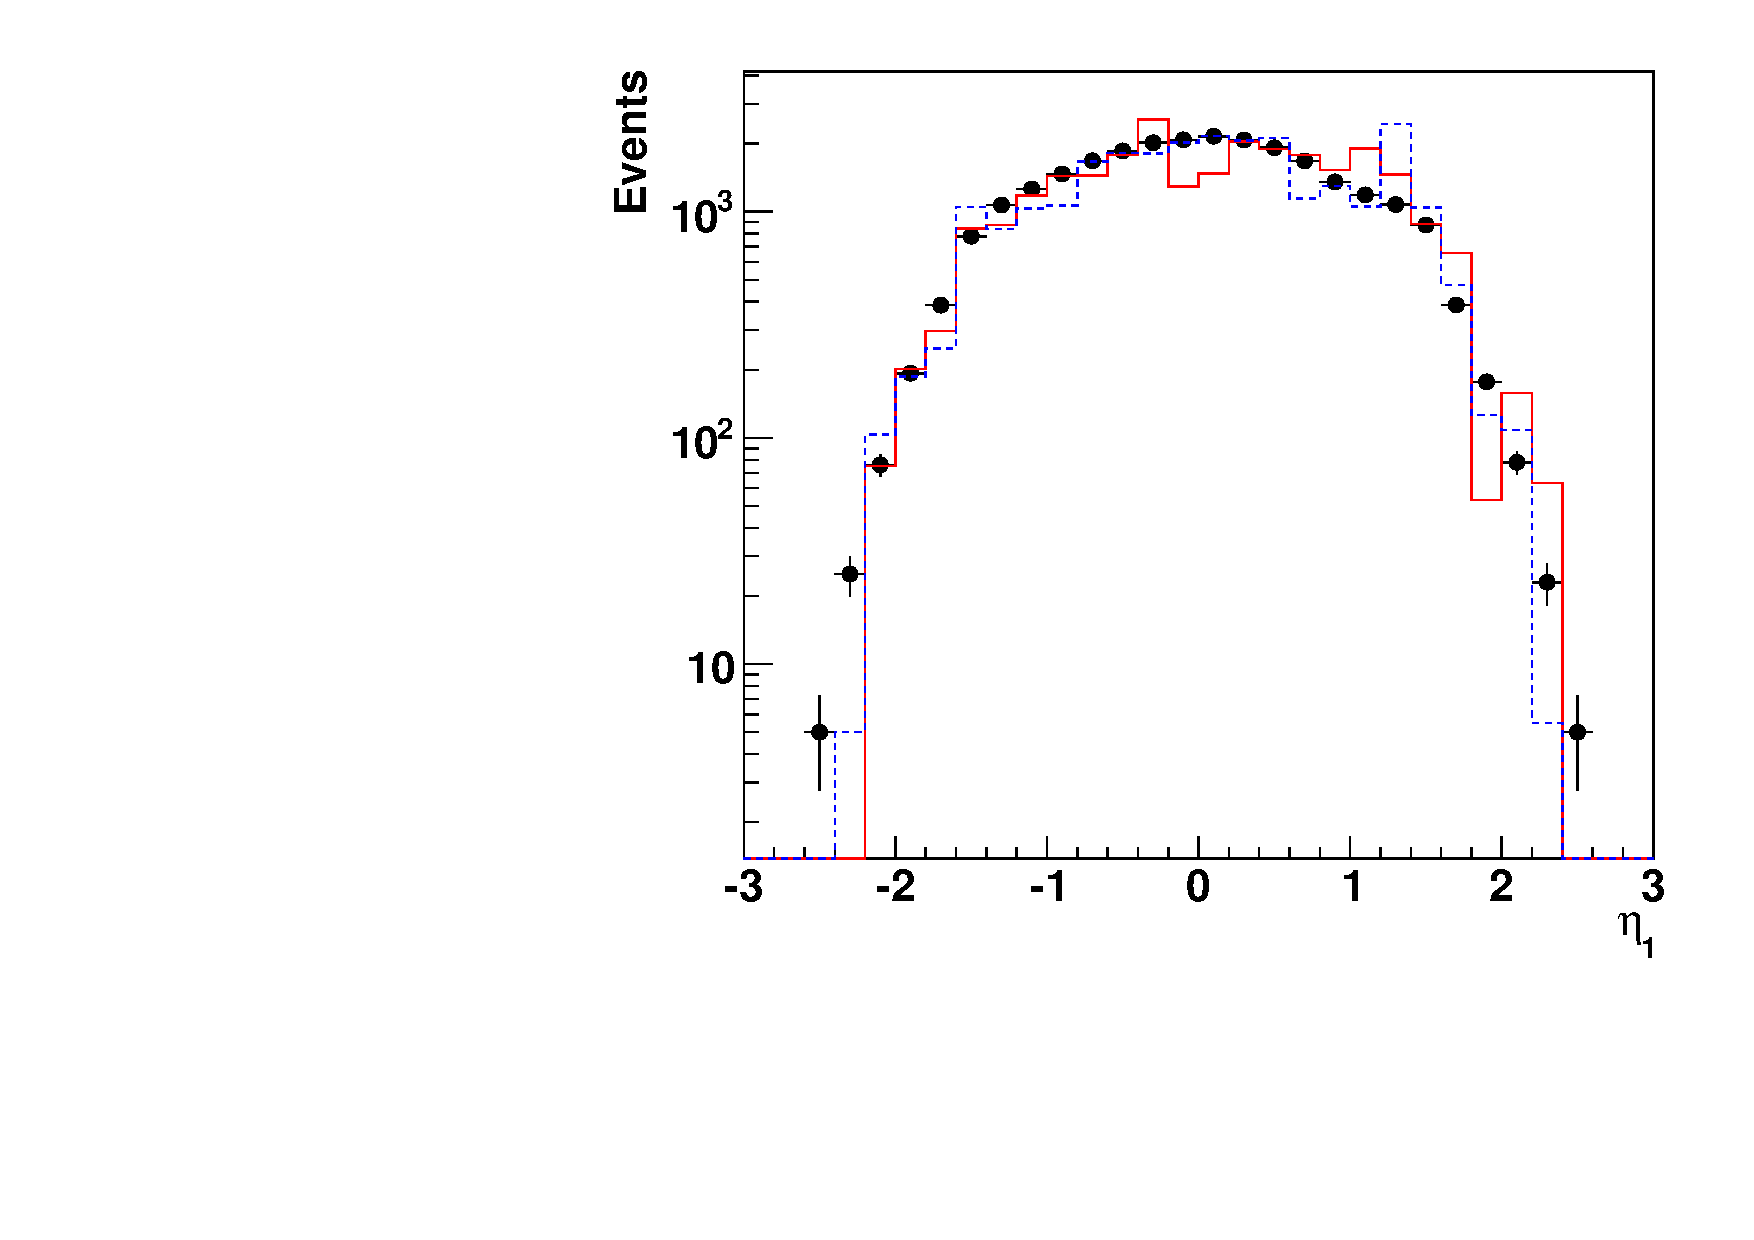
\includegraphics{figs/Data-MC-comparisons/Eta1-VVLowP.pdf}} &
     \resizebox{0.5\linewidth}{!}{\includegraphics{figs/Data-MC-comparisons/Eta1-VVMiumHigh.pdf}} \\
\end{tabular}
  \caption[Delta Eta Double]{Comparisons between data and Monte Carlo
                     for $\eta$ of the second leading jet of low purity (left) and low-high purity (right) 2-tagged events. The MC is normalized to the number of data events in each category. }
  \label{fig:Eta1Double}
\end{figure}

%\newpage
%\begin{figure}[htb]
%\centering
%\begin{tabular}{cc}
%     \resizebox{0.5\linewidth}{!}{\includegraphics{figs/Data-MC-comparisons/CA8CA8-qVLowP.pdf}} &
%     \resizebox{0.5\linewidth}{!}{\includegraphics{figs/Data-MC-comparisons/CA8CA8-qVMiumHigh.pdf}} \\
%\end{tabular}
%  \caption[PT Single]{Comparisons between data and Monte Carlo
%                    for $\Delta \phi$ of the leading ungroomed CA8 jet and leading pruned CA8 jet of low purity (left) and low-high purity (right) 1-tagged events.
%	   The MC is normalized to the number of data events in each category. }
%  \label{fig:CA8Single}
%\end{figure}

%\begin{figure}[htb]
%\centering
%\begin{tabular}{cc}
%     \resizebox{0.5\linewidth}{!}{\includegraphics{figs/Data-MC-comparisons/CA8CA8-VVLowP.pdf}} &
%     \resizebox{0.5\linewidth}{!}{\includegraphics{figs/Data-MC-comparisons/CA8CA8-VVMiumHigh.pdf}} \\
%\end{tabular}
%  \caption[PT Single]{Comparisons between data and Monte Carlo
%                    for $\Delta \phi$ of the leading ungroomed CA8 jet and leading pruned CA8 jet of low purity (left) and low-high purity (right) 2-tagged events.
%           The MC is normalized to the number of data events in each category. }
%  \label{fig:CA8Double}
%\end{figure}


\newpage
\begin{figure}[htb]
\centering
\begin{tabular}{cc}
     \resizebox{0.5\linewidth}{!}{\includegraphics{figs/Data-MC-comparisons/lumi19fb_dataMC_ca8jet_norm_mlog.pdf}} &
     \resizebox{0.5\linewidth}{!}{\includegraphics{figs/Data-MC-comparisons/data-qcd-Jet-Tau21.pdf}}\\
\end{tabular}
  \caption[Leading two jets mass]{Comparisons between data and Monte Carlo for
                    mass(left) and $\tau_{21}$(right) of the leading two jets.
	   The MC is normalized to the number of data events in each category.}
  \label{fig:massNsub}
\end{figure}



















\newpage

\begin{figure}[htb]
\centering
\begin{tabular}{cc}
     \resizebox{0.5\linewidth}{!}{\includegraphics{figs/Data-MC-comparisons/npv.pdf}} &
     \resizebox{0.5\linewidth}{!}{\includegraphics{figs/Data-MC-comparisons/npvlog.pdf}} \\
\end{tabular}
  \caption[Leading two jets mass drop]{Comparisons between data and Monte Carlo for
                   number of primary vertice to show the effect on Monte Carlo after pile up reweighting. 
	   The MC is normalized to the number of data events. Plot on the right is the log scale plot. (The plot includes only a subset of the full data sample.)}
  \label{fig:npv}
\end{figure}

\begin{figure}[htb]
\centering
\begin{tabular}{cc}
     \resizebox{0.5\linewidth}{!}{\includegraphics{figs/Data-MC-comparisons/neutralHadronEnergyFraction.pdf}} &
     \resizebox{0.5\linewidth}{!}{\includegraphics{figs/Data-MC-comparisons/neutralHadronEnergyFractionlog.pdf}} \\
\end{tabular}
  \caption[Leading two jets mass drop]{Comparisons between data and Monte Carlo for neutral hadron energy fraction.  
	   The MC is normalized to the number of data events. Plot on the right is the log scale plot. (The plot includes only a subset of the full data sample.)}
  \label{fig:neutralHadronEnergyFraction}
\end{figure}

\newpage

\begin{figure}[htb]
\centering
\begin{tabular}{cc}
     \resizebox{0.5\linewidth}{!}{\includegraphics{figs/Data-MC-comparisons/neutralEmEnergyFraction.pdf}} &
     \resizebox{0.5\linewidth}{!}{\includegraphics{figs/Data-MC-comparisons/neutralEmEnergyFractionlog.pdf}} \\
\end{tabular}
  \caption[Leading two jets mass drop]{Comparisons between data and Monte Carlo for neutral eletromagnetic energy fraction.  
	   The MC is normalized to the number of data events. Plot on the right is the log scale plot. (The plot includes only a subset of the full data sample.)}
  \label{fig:neutralEmEnergyFraction}
\end{figure}

\begin{figure}[htb]
\centering
\begin{tabular}{cc}
     \resizebox{0.5\linewidth}{!}{\includegraphics{figs/Data-MC-comparisons/chargedHadronEnergyFraction.pdf}} &
     \resizebox{0.5\linewidth}{!}{\includegraphics{figs/Data-MC-comparisons/chargedHadronEnergyFractionlog.pdf}} \\
\end{tabular}
  \caption[Leading two jets mass drop]{Comparisons between data and Monte Carlo for charged hadron energy fraction.  
	   The MC is normalized to the number of data events. Plot on the right is the log scale plot. (The plot includes only a subset of the full data sample.)}
  \label{fig:chargedHadronEnergyFraction}
\end{figure}

\newpage


\begin{figure}[htb]
\centering
\begin{tabular}{cc}
     \resizebox{0.5\linewidth}{!}{\includegraphics{figs/Data-MC-comparisons/chargedEmEnergyFraction.pdf}} &
     \resizebox{0.5\linewidth}{!}{\includegraphics{figs/Data-MC-comparisons/chargedEmEnergyFractionlog.pdf}} \\
\end{tabular}
  \caption[Leading two jets mass drop]{Comparisons between data and Monte Carlo for charged eletromagnetic energy fraction.  
	   The MC is normalized to the number of data events. Plot on the right is the log scale plot. (The plot includes only a subset of the full data sample.)}
  \label{fig:chargedEmEnergyFraction}
\end{figure}

\begin{figure}[htb]
\centering
\begin{tabular}{cc}
     \resizebox{0.5\linewidth}{!}{\includegraphics{figs/Data-MC-comparisons/chargedMultiplicity.pdf}} &
     \resizebox{0.5\linewidth}{!}{\includegraphics{figs/Data-MC-comparisons/chargedMultiplicitylog.pdf}} \\
\end{tabular}
  \caption[Leading two jets mass drop]{Comparisons between data and Monte Carlo for charged multiplicity.  
	   The MC is normalized to the number of data events. Plot on the right is the log scale plot. (The plot includes only a subset of the full data sample.)}
  \label{fig:chargedMultiplicity}
\end{figure}

\newpage

\begin{figure}[htb]
\centering
\begin{tabular}{cc}
     \resizebox{0.5\linewidth}{!}{\includegraphics{figs/Data-MC-comparisons/nConstituents.pdf}} &
     \resizebox{0.5\linewidth}{!}{\includegraphics{figs/Data-MC-comparisons/nConstituentslog.pdf}} \\
\end{tabular}
  \caption[Leading two jets mass drop]{Comparisons between data and Monte Carlo for number of constituents.  
	   The MC is normalized to the number of data events. Plot on the right is the log scale plot. (The plot includes only a subset of the full data sample.)}
  \label{fig:nConstituents}
\end{figure}


\begin{figure}[htb]
\centering
\begin{tabular}{cc}
     \resizebox{0.5\linewidth}{!}{\includegraphics{figs/Data-MC-comparisons/muonEnergyFraction.pdf}} &
     \resizebox{0.5\linewidth}{!}{\includegraphics{figs/Data-MC-comparisons/muonEnergyFractionlog.pdf}} \\
\end{tabular}
  \caption[Leading two jets mass drop]{Comparisons between data and Monte Carlo for the muon energy fraction of the leading two jets.  
	   The MC is normalized to the number of data events. Plot on the right is the log scale plot. (The plot includes only a subset of the full data sample.)}
  \label{fig:muonEnergyFraction}
\end{figure}

\newpage


%We find that the QCD MC agrees with data, although not perfect.
%For the dijet kinematics shown in Fig~\ref{fig:mjj},\ref{fig:dy},\ref{fig:dphi},\ref{fig:metSumPt},\ref{fig:jet1-pt},\ref{fig:jet2-pt},\ref{fig:eta of leading jet} and \ref{fig:eta of second leading jet}, we observe better agreement of Pythia6 $Z2*$ than Herwig++.
%For the jet substructure variables shown in Fig~\ref{fig:mass of leading two jets},\ref{fig:mass drop of leading two jets} and \ref{fig:subjet dR of leading two jets}, we observe that Herwig++ is better than Pythia $Z2*$.  
%In summary, Pythia6 $Z2*$ is more accurate at modelling the dijet kinematics,
%while Herwig++ models better the jet substructure.
We find that the QCD MC agrees with data, although not perfect.
For the dijet kinematics and also the jet substruture variables, we observe about the same agreement of Pythia6 $Z2*$ and Herwig++. 
For this analysis, we chose to model the background shape from the data itself
(as described below)
and depend on QCD MC only to provide us guidance and a cross check.

Fig~\ref{fig:dphiSingle}, Fig~\ref{fig:dphiDouble} and Fig~\ref{fig:metSumPtSingle} are particulariy useful to identify jets from calorimenter noise which would show up at low values of $\Delta\phi$ and high values of $E_{T}^{miss}/\sum E_{T}$. No enhencement in this region is observed which gives confidence that the applied noise filter cleaning and jet ID cuts leave no noise contamination within the two leading jets.

%Fig~\ref{fig:CA8Single} and Fig~\ref{fig:CA8Double} show the $\Delta \phi$ between the leading ungroomed CA8 jet and leading pruned CA8 jet.

%\begin{table}[htb]
%\begin{center}
%\begin{tabular}{|p{2.5cm}|p{2.5cm}|p{2.5cm}|p{2.5cm}|p{2.5cm}|}
%\begin{tabular}{|c|c|c|c|}
%\hline
%Categories & $\Delta \phi < 0.5(\%) $  & $0.5 < \Delta\phi < 2.0 (\%)$ & $2.0 < \Delta\phi (\%)$ \\
%\hline
%low purity 1-tag& 51.067 & 0.003 & 48.930 \\
%medium purity 1-tag&  90.458 & 0.002 & 9.541 \\
%high purity 1-tag & 95.156 & 0.001 & 4.844\\
%low purity 2-tag &  89.332 & 0.004 & 10.664 \\
%medium purity 2-tag& 90.636 & 0 & 9.363\\
%high purity 2-tag &  92.585 & 0 & 7.415\\
%\hline
%\end{tabular}
%\end{center}
%\caption{The ratio of the leading ungroomed CA8 jet matching to the leading pruned CA8 jet in different categories.}
%\label{table:matching}
%\end{table}


%Table~\ref{table:matching} shows the matching of the leading ungroomed CA8 jet and the leading pruned CA8 jet. 
%In the case of  $\Delta \phi<0.5$, the leading ungroomed CA8 jet  and leading pruned CA8 jet match.
%In the case of  $0.5 < \Delta \phi<2.0$, the leading ungroomed CA8 jet  and leading pruned CA8 jet don't match at all.
%In the case of  $\Delta \phi > 2.0$, the leading two jets are swapped and the leading ungroomed CA8 jet matches to the second leading pruned CA8 jet.

%Therefore there is no significant impact on the analyis from the fact that we use the leading two ungroomed CA8 jets to reconstruct the dijet mass while using the leading two pruned CA8 jets for W/Z-tagging of events.

Fig~\ref{fig:npv} shows the number of primary vertices distribution after pile up reweighting on the MC. 
Fig~\ref{fig:neutralHadronEnergyFraction}, Fig~\ref{fig:neutralEmEnergyFraction}, Fig~\ref{fig:chargedHadronEnergyFraction}, Fig~\ref{fig:chargedEmEnergyFraction}, Fig~\ref{fig:chargedMultiplicity} and Fig~\ref{fig:nConstituents} show the jet ID variable distribution after the event selection, and Fig~\ref{fig:muonEnergyFraction}, the muon energy faction of the leading two jets.

\clearpage

\clearpage
\section{W-tagging scale factor}

We derive the scale factor for the $\tau 2/\tau 1$ W tagger, in both the tight and loose regions, by
comparing its efficiency in semileptonic $t\overline{t}$ events, both
in data and mote carlo. We isolate the W candidates with kinematic
cuts. We consider only muon events. We then apply the tagger and require the W mass to be within
$70$ and $100~\GeVcc$.

In Monte Carlo, we attempt to match the CA8 jets to real Ws by
requiring that the daughters of a hadronic W from the particle generator lie within a
cone of $\Delta R < 0.3$ of a jet's subjets. Jets that meet this
requirement are ''matched'' jets. We can then classify all W
candidates in the following ways:
\begin{enumerate}
\item Matched W jets which pass the tight $\tau 2/\tau 1$ cut.
\item Matched W jets which pass the loose $\tau 2/\tau 1$ cut.
\item Matched W jets which fail both $\tau 2/\tau 1$ cuts.
\item Unmatched W jets which pass the tight $\tau 2/\tau 1$ cut.
\item Unmatched W jets which pass the loose $\tau 2/\tau 1$ cut.
\item Unmatched W jets which fail both $\tau 2/\tau 1$ cuts.
\end{enumerate}
The efficiency for either tight or loose can be extracted by counting the number of matched
W jets in that region and dividing by the total number of
matched W jets.

We derive the efficiency in data by simultaneously fitting the
W mass distributions of the events in the tight, loose and failed events. The general shapes of the distributions are taken from MC. The efficiencies are explicit fit parameters which relate the normalizations of categories category. We must also take into account small background contributions from non-$t\overline{t}$ sources. These contributions are also parametrized as shapes and included in the fit.

\subsection{Fit to monte carlo}

We first find the PDFs associated with each of the event categories
above by fitting their distributions from the Monte Carlo, 
as follows:
\begin{itemize}
\item {\bf Tight, Matched Jets} We fit the tight matched events with the sum of two gaussians.
\item {\bf Loose, Matched Jets} We fir the loose matched events with a sum of the double-gaussian found in the tight selection and an exponential.
\item {\bf Failed, Matched Jets} We fit failed matched events with an exponential.
\item {\bf Tight, Unatched Jets} We fit tight unmatched events with the sum of a gaussian and a linear function with positive slope.
\item {\bf Loose, Unatched Jets} We fit loose unmatched events with a gaussian.
\item {\bf Failed, Unatched Jets} We fit failed unmatched events with an exponential.
\item {\bf Backgrounds} All backgrounds are fit with gaussians in the tight and loose regions, and an exponential in the failed region. These shapes are added to the respective unmatched shapes to derive a total non-matched shape.
\end{itemize}
Fits to matched and unmatched distributions are shown in figures \ref{fig:fitsmatched} and \ref{fig:fitsunmatched}.
%\includegraphics[width=0.35\textwidth]{figs/limits/brazilianFlag_qW_high_purity.pdf}%
\begin{figure}[h!]
\centering
                \includegraphics[width=0.32\textwidth]{EXO-12-024/figs/WtagSF/MT.pdf}
                \includegraphics[width=0.32\textwidth]{EXO-12-024/figs/WtagSF/ML.pdf}
                \includegraphics[width=0.32\textwidth]{EXO-12-024/figs/WtagSF/MF.pdf}
\caption{Fits to matched $t\overline{t}$ distributions. Left: tight region. Center: loose region. Right: failed events.}\label{fig:fitsmatched}
\end{figure}

\begin{figure}[h!]
\centering
                \includegraphics[width=0.32\textwidth]{EXO-12-024/figs/WtagSF/UT.pdf}
                \includegraphics[width=0.32\textwidth]{EXO-12-024/figs/WtagSF/UL.pdf}
                \includegraphics[width=0.32\textwidth]{EXO-12-024/figs/WtagSF/UF.pdf}
\caption{Fits to unmatched $t\overline{t}$ distributions. Left: tight region. Center: loose region. Right: failed events.}\label{fig:fitsunmatched}
\end{figure}

\subsubsection{Fits to data}
We fit the above shapes to the data. The following parameters are kept constant, with their values taken form the MC fits described in the previous section:
\begin{enumerate}
\item In the unmatched and background distrubtions
	\begin{enumerate}
	\item The relative normalization of the gaussian and linear components of the tight, unmatched shape.
	\item The position of the gaussian peak in the loose, unmatched distribution is fixed.
	\item The means and standard deviations, as well as the decay coefficients of all backgrounds are fixed, but their normalizations are not.
	\end{enumerate}
\item In the matched distributions
        \begin{enumerate}
	\item The relative normalization of the two gaussians in the tight region is fixed.
	\item The relative position (as a multiplier) of the two gaussian peaks is fixed.
	\item The relative normalization of the exponential and double-gaussian shapes in the loose region is fixed.
        \end{enumerate}
\end{enumerate}

All other parameters are allowed to float. All other normalizations are parametrized in terms of the efficiency. The results of the fits to data are shown in figure \ref{fig:datafits}. As a consistency check, the same proceedure is applied to the MC distribution. The result of that fit is shown in figure \ref{fig:mcfits}.
\begin{figure}[h!]
\centering
        \includegraphics[width=0.49\textwidth]{EXO-12-024/figs/WtagSF/MCTIGHT.pdf}
	\includegraphics[width=0.49\textwidth]{EXO-12-024/figs/WtagSF/MCLOOSE.pdf}
        \caption{Distributions from data of $W$ mass in the tight (left) and loose (right) $\tau_2/\tau_1$ regions, and resulting fits.}\label{fig:datafits}
\end{figure}
\begin{figure}[h!]
\centering
        \includegraphics[width=0.49\textwidth]{EXO-12-024/figs/WtagSF/TIGHT.pdf}
	\includegraphics[width=0.49\textwidth]{EXO-12-024/figs/WtagSF/LOOSE.pdf}
        \caption{Distributions from MC of $W$ mass in the tight (left) and loose (right) $\tau_2/\tau_1$ regions, and resulting fits.}\label{fig:mcfits}
\end{figure}

More details on the fitting procedure and the $t\overline{t}$ selection can be found in the appendix of this note.

\subsection{Scale factor measurement}
We measure the scale factor of the $\tau 2/\tau 1$ cut efficiency and that of the W mass window $70$ to $100\GeVcc$ efficiency. We find that the total scale factor for the two cuts is $0.860 \pm 0.065$ in the tight region and $138.5 \pm 75.2$ in the loose region.

\subsubsection{Related systematics}
The errors in the scale factors are found from the fitting errors and systematic errors from the choice of fixed parameters. Each fixed parameter found in MC is varied by its fitting error and used to generate toy MC to which the fitting proceedure is applied. The resulting offset is taken to be the systematic error from this fixed parameter. In addition, when the efficiency from a fit to MC differs with that from MC truth information, we take the difference to be an additional systematic. 
Additional systematic uncertainties on the W-tagging efficiency related to detector effects are discussed in the systematics section of this note.
\clearpage

\section{The signal: dijet resonance}
\label{sec:signal}

We search for dijet resonances corresponding to several models.
Using the W/Z-tagging algorithm, we examine both single W/Z-tag and double W/Z-tag events.

The pruned jet mass and jet $\tau_{21}$ distributions in signal MC, data and background MC are shown in Figure~\ref{fig:taggingvariables}.
Fully merged jets from W and Z decays peak around 80$\sim$90\GeVcc while QCD jets and not fully merged W and Z jets peak around 20\GeVcc.
The discriminating power of the pruned jet mass and $\tau_{21}$ is evident.

For both the pruned jet mass and $\tau_{21}$, differences are observed
between the \HERWIG{++} ($G_{RS}$) and \PYTHIA~6
($G_{Bulk}$, $\cPq^*$, $\PWpr$) distributions, which arise from
differences in the polarization of the $\PW$/$\cPZ$ boson and the
showering and hadronization models used by these generators. 
%In
%particular this is the reason why the $\PW\cPZ$ prediction for
%$\tau_{21}$ is different from the $\PW\PW$, $\cPZ\cPZ$ predictions.
The differences, due to showering and hadronization,
are taken into account in estimating the systematic uncertainties
on the tagging efficiencies, as discussed below.

\begin{figure}[htb]
\begin{center}
\includegraphics[width=0.49\textwidth]{EXO-12-024/figs/signal-acc-eff/signal-data-qcd-jetmass.pdf}
\includegraphics[width=0.49\textwidth]{EXO-12-024/figs/signal-acc-eff/signal-data-qcd-Jet-Tau21.pdf}
\end{center}
\caption{Pruned jet mass and $\tau_{21}$ in signal MC, data and background MC.
All curves are plotted with the same binning.
The signal MC distributions are plotted as smooth curves connecting the histogram entries. MCs are normalized according to data.
}
\label{fig:taggingvariables}
\end{figure}

%Table~\ref{table:acceptance} summarizes the signal branching ratio times angular acceptances and also the W/Z-tagging efficiencies.

The full event selection efficiency is estimated using simulated
signal samples.
Less than 1\% of the $\cPZ\cPZ$ or $\PW\PW$ events which pass the full
selection are from $\cPZ\cPZ \to ll qq$ or $\PW\PW \to l\nu qq$
decays, where $l$ can be a muon or electron.  While 3\% of the
selected $\cPZ\cPZ$ events are from $\cPZ\cPZ \to \tau\tau qq$ decays,
less than 1\% of the selected $\PW\PW$ events are from $\PW\PW \to
\tau\nu qq$ decays.
To within 10\% accuracy the full selection efficiency can
therefore be
approximated by the product of the $\PW/\cPZ$-tagging efficiency
and an approximate acceptance.
This acceptance is shown in Figure~\ref{fig:acceptances} and
takes into account the angular acceptance
($|\eta| < 2.5$, $|\Delta\eta|<1.3$),
the branching into quark final states,
$\mathcal{B}$($\PW/\cPZ \to \text{quarks}$) and a matching within
$\Delta R = \sqrt{(\Delta \eta)^2 + (\Delta\phi)^2} <0.5$
between the generated W/Z bosons and the reconstructed jets.


%\begin{table}[htbp]
%\begin{tabular}{|l|l|r|r|l|l|r|r|}
%\hline
%signal  & model & mass & BR($W/Z \to jets$)$\times$acc. & M 1-tag & H 1-tag & M 2-tag & H 2-tag \\ \hline
%$G_{RS} \to WW$ & Herwig++ & 1000 & 0.382 & NAN & NAN & 0.073 & 0.116 \\ 
%$G_{RS} \to WW$ & Herwig++ & 1500 & 0.401 & NAN & NAN & 0.076 & 0.092 \\ 
%$G_{RS} \to WW$ & Herwig++ & 1800 & 0.403 & NAN & NAN & 0.082 & 0.089 \\ 
%$G_{RS} \to WW$ & Herwig++ & 2000 & 0.404 & NAN & NAN & 0.076 & 0.079 \\ 
%$G_{RS} \to WW$ & Herwig++ & 2500 & 0.411 & NAN & NAN & 0.055 & 0.046 \\ 
%$G_{RS} \to WW$ & Herwig++ & 3000 & 0.409 & NAN & NAN & 0.032 & 0.029 \\ \hline 
%$G_{RS} \to ZZ$ & Herwig++ & 1000 & 0.390 & NAN & NAN & 0.070 & 0.120 \\ 
%$G_{RS} \to ZZ$ & Herwig++ & 1500 & 0.391 & NAN & NAN & 0.088 & 0.119 \\ 
%$G_{RS} \to ZZ$ & Herwig++ & 1800 & 0.387 & NAN & NAN & 0.095 & 0.125 \\ 
%$G_{RS} \to ZZ$ & Herwig++ & 2000 & 0.383 & NAN & NAN & 0.095 & 0.121 \\ 
%$G_{RS} \to ZZ$ & Herwig++ & 3000 & 0.374 & NAN & NAN & 0.077 & 0.056 \\ \hline
%$G_{RS} \to WW$ & Pythia Z2* & 1000 & 0.455 & NAN & NAN & 0.081 & 0.132 \\ 
%$G_{RS} \to WW$ & Pythia Z2* & 1500 & 0.432 & NAN & NAN & 0.088 & 0.124 \\ 
%$G_{RS} \to WW$ & Pythia Z2* & 1800 & 0.419 & NAN & NAN & 0.079 & 0.109 \\ 
%$G_{RS} \to WW$ & Pythia Z2* & 2000 & 0.415 & NAN & NAN & 0.078 & 0.094 \\ 
%$G_{RS} \to WW$ & Pythia Z2* & 2500 & 0.397 & NAN & NAN & 0.059 & 0.056 \\ 
%$G_{RS} \to WW$ & Pythia Z2* & 3000 & 0.391 & NAN & NAN & 0.040 & 0.035 \\ \hline
%$G_{RS} \to ZZ$ & Pythia Z2* & 1000 & 0.454 & NAN & NAN & 0.075 & 0.149 \\ 
%$G_{RS} \to ZZ$ & Pythia Z2* & 1500 & 0.417 & NAN & NAN & 0.106 & 0.161 \\ 
%$G_{RS} \to ZZ$ & Pythia Z2* & 1800 & 0.400 & NAN & NAN & 0.107 & 0.154 \\ 
%$G_{RS} \to ZZ$ & Pythia Z2* & 2000 & 0.389 & NAN & NAN & 0.113 & 0.148 \\ 
%$G_{RS} \to ZZ$ & Pythia Z2* & 3000 & 0.355 & NAN & NAN & 0.081 & 0.071 \\ \hline
%$W' \to WZ$ & Pythia Z2* & 1000 & 0.486 & NAN & NAN & 0.109 & 0.246 \\ 
%$W' \to WZ$ & Pythia Z2* & 1500 & 0.487 & NAN & NAN & 0.121 & 0.246 \\ 
%$W' \to WZ$ & Pythia Z2* & 1800 & 0.485 & NAN & NAN & 0.119 & 0.216 \\ 
%$W' \to WZ$ & Pythia Z2* & 2000 & 0.484 & NAN & NAN & 0.117 & 0.199 \\ 
%$W' \to WZ$ & Pythia Z2* & 2200 & 0.479 & NAN & NAN & 0.108 & 0.172 \\ 
%$W' \to WZ$ & Pythia Z2* & 2500 & 0.485 & NAN & NAN & 0.092 & 0.139 \\ 
%$W' \to WZ$ & Pythia Z2* & 3000 & 0.494 & NAN & NAN & 0.068 & 0.114 \\ \hline
%$q* \to qW$ & Pythia Z2* & 1000 & 0.502 & 0.125 & 0.364 & NAN & NAN \\ 
%$q* \to qW$ & Pythia Z2* & 1500 & 0.495 & 0.135 & 0.333 & NAN & NAN \\ 
%$q* \to qW$ & Pythia Z2* & 2000 & 0.497 & 0.139 & 0.306 & NAN & NAN \\ 
%$q* \to qW$ & Pythia Z2* & 3000 & 0.490 & 0.129 & 0.177 & NAN & NAN \\ 
%$q* \to qW$ & Pythia Z2* & 4000 & 0.475 & 0.121 & 0.130 & NAN & NAN \\ \hline
%$ q* \to qZ$ & Pythia Z2* & 1000 & 0.494 & 0.116 & 0.371 & NAN & NAN \\ 
%$ q* \to qZ$ & Pythia Z2* & 1500 & 0.488 & 0.138 & 0.384 & NAN & NAN \\ 
%$ q* \to qZ$ & Pythia Z2* & 2000 & 0.474 & 0.154 & 0.364 & NAN & NAN \\ 
%$ q* \to qZ$ & Pythia Z2* & 3000 & 0.452 & 0.173 & 0.262 & NAN & NAN \\ 
%$ q* \to qZ$ & Pythia Z2* & 4000 & 0.449 & 0.156 & 0.187 & NAN & NAN \\ \hline
%\end{tabular}
%\caption{Summary of signal branching ratio times angular acceptance and W/Z-tagging efficiency, in medium purity 1-tag, high purity 
%1-tag, medium purity 2-tag and high purity 2-tag categories. }
%\label{table:acceptance}
%\end{table}
%






%\begin{table}[htb]
%\begin{center}
%\begin{tabular}{ |c|c|c|c|c|c| }
%\hline
%signal & model & mass & BR($W/Z \to jets$)$\times$acc. & 1 W/Z-tag & 2 W/Z-tag\\
%\hline
%hline
%\end{tabular} 
%\end{center}
%\caption{Summary of signal branching ratio times acceptance and W/Z-tagging efficiency.}
%\label{table:acceptance}
%\end{table}

\begin{figure}[htb]
\begin{center}
\includegraphics[width=0.88\textwidth]{EXO-12-024/figs/signal-acc-eff/all-signal-acc-8TeV.pdf}
\end{center}
\caption{Fraction of events with branching into quark final states, BR($\PW/\cPZ \to \text{quarks}$),
  which are reconstructed as dijets ($\text{quarks} \to \text{jets}$)
  and pass the angular acceptance ($|\eta| < 2.5$, $|\Delta\eta|<1.3$.}
\label{fig:acceptances}
\end{figure}

\begin{figure}[htb]
\begin{center}
\includegraphics[width=0.49\textwidth]{EXO-12-024/figs/signal-acc-eff/single-tagging-eff-medium.pdf}
\includegraphics[width=0.49\textwidth]{EXO-12-024/figs/signal-acc-eff/single-tagging-eff.pdf}
\end{center}
\caption{The fraction of singly-tagged events, requiring one medium purity (left) 
  and high purity (right) $\PW/\cPZ$-tag in data,
  signal and background simulations for events passing the angular acceptance
  requirement ($|\eta| < 2.5$, $|\Delta\eta|<1.3$).}
\label{fig:singleefficiencies}
\end{figure}

\begin{figure}[htb]
\begin{center}
\includegraphics[width=0.49\textwidth]{EXO-12-024/figs/signal-acc-eff/double-tagging-eff-medium.pdf}
\includegraphics[width=0.49\textwidth]{EXO-12-024/figs/signal-acc-eff/double-tagging-eff.pdf}
\end{center}
\caption{The fraction of doubly-tagged events, requiring two medium purity (left) 
and high purity (right) $\PW/\cPZ$-tags in data,
  signal and background simulations for events passing the angular acceptance
  requirement ($|\eta| < 2.5$, $|\Delta\eta|<1.3$).}
\label{fig:doubleefficiencies}
\end{figure}
%


The W/Z-tagging efficiency and also the tag rate in data are shown in Figure~\ref{fig:singleefficiencies} and Figure~\ref{fig:doubleefficiencies}. Since data is dominated by background events, the tag rate
in data could be viewed as mistag rate. 
%The W/Z-tagging efficiency for single W/Z-tagged signals is about $13\% - 38\%$ in high purity category, and $12\% - 18\%$ in medium purity category.
%The W/Z-tagging efficiency for a double W/Z-tagged signals is about $3\% - 12\%$ in high purity category, and $3\% - 9\%$ in medium purity category.


The signal shapes for all five processes considered in this analysis are shown in Figure~\ref{fig:mediumsignalShapes} and Figure~\ref{fig:highsignalShapes}.  
For the qW and qZ final states, the shape with a single W/Z-tag required is shown, while for the other signals two W/Z-tags are required.


%Fig~\ref{fig:acceptanceGstarWWherwig} and Fig~\ref{fig:acceptanceGstarWWpythia} show the signal shape for process: $G_{RS} \to WW$.
%Fig~\ref{fig:acceptanceGstarZZherwig} and Fig~\ref{fig:acceptanceGstarZZpythia} show the signal shape for process: $G_{RS} \to ZZ$.  
%Fig~\ref{fig:acceptanceWprime} shows the signal shape for process: $W' \to WZ$. 
%Fig~\ref{fig:acceptanceqstarqW} and Fig~\ref{fig:acceptanceqstarqZ} shows the signal shape for process: $q* \to qW$, $qZ$.
%The different line colors correspond to different signal resonance masses.
%The dashed line is for signal with a single W/Z-tag, while the dotted 
%line is for signal with two W/Z-tags.

\begin{figure}[htb]
\begin{center}
\includegraphics[width=0.75\textwidth]{EXO-12-024/figs/signal-acc-eff/resonance-shape-medium.pdf}
\end{center}
\caption{The normalized medium purity signal resonance distribution for  $G_{RS}\to WW$, $G_{RS}\to ZZ$, $W' \to WZ$, $q*\to qW$, and $q*\to qZ$ resonances of dijet invariant mass 1.0\TeVcc, 1.5\TeVcc, 2.0\TeVcc, 2.5 \TeVcc,  3.0\TeVcc, 4.0\TeVcc.
}
\label{fig:mediumsignalShapes}
\end{figure}


\begin{figure}[htb]
\begin{center}
\includegraphics[width=0.75\textwidth]{EXO-12-024/figs/signal-acc-eff/resonance-shape.pdf}
\end{center}
\caption{The normalized high purity signal resonance distribution for  $G_{RS}\to WW$, $G_{RS}\to ZZ$, $W' \to WZ$, $q*\to qW$, and $q*\to qZ$ resonances of dijet invariant mass 1.0\TeVcc, 1.5\TeVcc, 2.0\TeVcc,  3.0\TeVcc, 4.0\TeVcc.
}
\label{fig:highsignalShapes}
\end{figure}

%\begin{figure}[htb]
%\begin{center}
%\includegraphics[width=0.75\textwidth]{EXO-12-024/figs/signal-acc-eff/resonance-shape-double-1500.pdf}
%\end{center}
%\caption{The normalized signal resonance distribution of Herwig++ and Pythia6 Z2* for 1.5 \TeVcc $G_{RS}\to \wboson\wboson$, $G_{RS}\to \zboson\zboson$ resonances of dijet invariant mass.
%}
%\label{fig:signalShapes2}
%\end{figure}




%\begin{figure}[htb]
%\begin{center}
%\includegraphics[width=0.48\textwidth]{EXO-12-024/figs/signal-acc-eff/GstarWWherwig.pdf}
%\includegraphics[width=0.48\textwidth]{EXO-12-024/figs/signal-acc-eff/RSGWWherwig-deta.pdf}
%\end{center}
%\caption{Signal shape in AK5 dijet mass and $\Delta \eta$: $G_{RS} \to WW$ using Herwig++.
%The shape in AK5 dijet mass is normalized to the number of generated events (with phasespace cuts).
%The distribution in $\Delta \eta$ is normalized to the number of events passing the analysis selection in the inclusive category (no W/Z-tagging required).} 
%\label{fig:acceptanceGstarWWherwig}
%\end{figure}


%\begin{figure}[htb]
%\begin{center}
%\includegraphics[width=0.48\textwidth]{EXO-12-024/figs/signal-acc-eff/GstarWWpythia.pdf}
%\includegraphics[width=0.48\textwidth]{EXO-12-024/figs/signal-acc-eff/RSGWWpythia-deta.pdf}
%\end{center}
%\caption{Signal shape in AK5 dijet mass and $\Delta \eta$: $G_{RS} \to WW$ using Pythia Z2*.
%The shape in AK5 dijet mass is normalized to the number of generated events (with phasespace cuts).
%The distribution in $\Delta \eta$ is normalized to the number of events passing the analysis selection in the inclusive category (no W/Z-tagging required).}
%\label{fig:acceptanceGstarWWpythia}
%\end{figure}

%\begin{figure}[htb]
%\begin{center}
%\includegraphics[width=0.48\textwidth]{EXO-12-024/figs/signal-acc-eff/GstarZZherwig.pdf}
%\includegraphics[width=0.48\textwidth]{EXO-12-024/figs/signal-acc-eff/RSGZZherwig-deta.pdf}
%\end{center}
%\caption{Signal shape in AK5 dijet mass and $\Delta \eta$: $G_{RS} \to ZZ$ using Herwig++.
%The shape in AK5 dijet mass is normalized to the number of generated events (with phasespace cuts).
%The distribution in $\Delta \eta$ is normalized to the number of events passing the analysis selection in the inclusive category (no W/Z-tagging required).}
%\label{fig:acceptanceGstarZZherwig}
%\end{figure}



%\begin{figure}[htb]
%\begin{center}
%\includegraphics[width=0.48\textwidth]{EXO-12-024/figs/signal-acc-eff/GstarZZpythia.pdf}
%\includegraphics[width=0.48\textwidth]{EXO-12-024/figs/signal-acc-eff/RSGZZpythia-deta.pdf}
%\end{center}
%\caption{Signal shape in AK5 dijet mass and $\Delta \eta$: $G_{RS} \to ZZ$ using Pythia Z2*.
%The shape in AK5 dijet mass is normalized to the number of generated events (with phasespace cuts).
%The distribution in $\Delta \eta$ is normalized to the number of events passing the analysis selection in the inclusive category (no W/Z-tagging required).}
%\label{fig:acceptanceGstarZZpythia}
%\end{figure}


%\begin{figure}[htb]
%\begin{center}
%\includegraphics[width=0.48\textwidth]{EXO-12-024/figs/signal-acc-eff/WZWprime.pdf}
%\includegraphics[width=0.48\textwidth]{EXO-12-024/figs/signal-acc-eff/Wprime-deta.pdf}
%\end{center}
%\caption{Signal shape in AK5 dijet mass and $\Delta \eta$: $W' \to WZ$.
%The shape in AK5 dijet mass is normalized to the number of generated events (with phasespace cuts).
%The distribution in $\Delta \eta$ is normalized to the number of events passing the analysis selection in the inclusive category (no W/Z-tagging required).}
%\label{fig:acceptanceWprime}
%\end{figure}

%\begin{figure}[htb]
%\begin{center}
%\includegraphics[width=0.48\textwidth]{EXO-12-024/figs/signal-acc-eff/qstarqw.pdf}
%\includegraphics[width=0.48\textwidth]{EXO-12-024/figs/signal-acc-eff/QstarToQW-deta.pdf}
%\end{center}
%\caption{Signal shape in AK5 dijet mass and $\Delta \eta$: $q*\to qW$.
%The shape in AK5 dijet mass is normalized to the number of generated events (with phasespace cuts).
%The distribution in $\Delta \eta$ is normalized to the number of events passing the analysis selection in the inclusive category (no W/Z-tagging required).}
%\label{fig:acceptanceqstarqW}
%\end{figure}

%\begin{figure}[htb]
%\begin{center}
%\includegraphics[width=0.48\textwidth]{EXO-12-024/figs/signal-acc-eff/qstarqz.pdf}
%\includegraphics[width=0.48\textwidth]{EXO-12-024/figs/signal-acc-eff/QstarToQZ-deta.pdf}
%\end{center}
%\caption{Signal shape in AK5 dijet mass and $\Delta \eta$: $q*\to qZ$.
%The shape in AK5 dijet mass is normalized to the number of generated events (with phasespace cuts).
%The distribution in $\Delta \eta$ is normalized to the number of events passing the analysis selection in the inclusive category (no W/Z-tagging required).}
%\label{fig:acceptanceqstarqZ}
%\end{figure}


\clearpage


\section{Systematic uncertainties}
\label{sec:systematics}
The sources of systematic uncertainties are summarized as
follows:
\begin{itemize}
\item Background-related systematic uncertainties: background parametrization.
\item Signal-related systematics uncertainties: W/Z-tagging efficiency, Jet Energy Scale(JES), Jet Energy Resolution(JER), luminosity.
\end{itemize}

\subsection{Background shape parametrization}
\label{sec:background}

We model the shape of the QCD background in the dijet spectrum 
using a simple parametrization which has been sucessfully deployed in
previous searches in the dijet mass spectrum~\cite{cmsdijet}.
The background model is given in Eq.~(\ref{eqParam}):
\begin{equation}
\frac{{\rm d}N}{{\rm d}m} = 
\frac{P_{0} (1 - m/\sqrt{s})^{P_{1}}}{(m/\sqrt{s})^{P_{2}
}} .
\label{eqParam}
\end{equation}
\noindent where $m$ denotes the dijet mass and $\sqrt{s}$ the pp center of mass energy.
$P_0$ acts as a normalization parameter for the probability
density function, and $P_1$, $P_2$ describe its shape.
It was checked by a Fisher F-test that no additional parameter is not needed to discribe the distributions.

Figure \ref{fig:singleVtagBG} and Figure \ref{fig:doubleVtagBG} show the dijet mass spectra from
single and double $\PW/\cPZ$-tagged data fitted to Eq.~(\ref{eqParam}) and the bottom panes show corresponding pull
distributions, demonstrating the agreement between the background-only
probability density function and the data.

No sizeable deviation from the background-only hypothesis is seen,
exclusion limits are set on the product of cross section, acceptance, and branching fraction for
the five considered final states: qW, qZ, WW, WZ, and ZZ.

\begin{figure}[th!b]
\begin{center}
\includegraphics[width=0.49\textwidth]{figs/MediumPuriqVFitAndPull.pdf}
\includegraphics[width=0.49\textwidth]{figs/HighPuriqVFitAndPull.pdf}
\end{center}
\caption{The medium purity (\cmsLeft) and high purity (\cmsRight) single $\PW/\cPZ$-tagged $m_{jj}$
  distributions (points) in data fitted with the QCD background parametrization (solid
  curve).  Signal shape distribution for $\cPq^* \to \cPq\PW$
   with its corresponding cross section is also shown.  Bottom panes:
  the corresponding pull distributions ($\frac{\text{Data}-\text{Fit}}{\sigma_{\text{Data}}}$).  }
\label{fig:singleVtagBG}
\end{figure}

\begin{figure}[th!b]
\begin{center}
\includegraphics[width=0.49\textwidth]{figs/MediumPuriVVFitAndPull.pdf}
\includegraphics[width=0.49\textwidth]{figs/HighPuriVVFitAndPull.pdf}
\end{center}
\caption{The medium purity (\cmsLeft) and high purity (\cmsRight) double $\PW/\cPZ$-tagged $m_{jj}$
  distributions (points) in data fitted with the QCD background parametrization (solid
  curve).  Signal shape distribution for
  $\GRS \to \PW\PW$ with its corresponding cross section is also shown.  Bottom panes:
  the corresponding pull distributions ($\frac{\text{Data}-\text{Fit}}{\sigma_{\text{Data}}}$).  }
\label{fig:doubleVtagBG}
\end{figure}



\subsection{W/Z-tagging efficiency}
\label{sec:vtageff}

The W/Z-tagging efficiency is determined from the Monte Carlo simulation.
We cross-check the MC modelling of the signal efficiency by measuring the W/Z-tagging efficiency
in semileptonic $\ttbar$ data, and compare it
with the same efficiency obtained using identical procedure from $\ttbar$ Monte Carlo sample generated with MadGraph~\cite{madgraph} and showered with Pythia6 Tune Z2*.
The ratio of the two efficiencies defines a scale factor, which is then applied to
the efficiencies for signals in the dijet data.

We follow the same procedure as described in Ref.~\cite{JME-13-006}.
%The efficiency of the cut on the $\tau_{21}$ variable in the semileptonic $\ttbar$ sample is found to be \mucuteffsemilepdata for data, %and \mucuteffsemilepmc for Monte Carlo.
%The efficiency of the pruned jet mass cut for the data and Monte Carlo are \mcuteffsemilepdata and \mcuteffsemilepmc, respectively.
Combining the efficiencies of the $\tau_{21}$ and jet mass cuts, a data-MC scale factor of  \scalefactorHP
(\scalefactorLP) for the high (low) purity selection for the  W-tagging efficiency is determined.
We assume that the same scale factor applies to \zboson-tagging as well.
The errors on the scale factor are propagated
into the systematic uncertainties on the overal signal efficiency.


%\begin{figure}[htb]
%\centering
%\includegraphics[width=0.95\textwidth]{figs/semiLepMass_muHist}
%\caption{$\tau_{21}$ of the highest mass jet in a semileptonic
%ttbar sample from Ref.~\cite{hadronictop}.}
%\label{figs:muHist_semileptonic}
%\end{figure}

%\begin{figure}[htbp]
%\centering
%\includegraphics[width=0.95\textwidth]{figs/semiLepMass_mWCand.pdf}
%\caption{Pruned jet mass of the highest mass jet in a semileptonic
%ttbar sample from Ref.~\cite{hadronictop}.}
%\label{figs:mHist_semileptonic}
%\end{figure}


The efficiency error on a single $\PW/\cPZ$-tagging is estimated with
a control sample of semileptonic $t \bar t$ events as described above.
The uncertainties of \scalefactorHPu (\scalefactorLPu) on the scale
factors for high (low) purity tagging include sources from control
sample statistics, pruned jet mass scale and pruned jet mass
resolution.
Since we estimate the scale factor
only in the kinematic regime of the $\ttbar$ sample where the W decay
products merge, but the b-quarks are still reconstructed as separate
jets, we need to rely on the simulation to extrapolate to
higher jet \pt.
Therefore, we estimate how the efficiency varies as a function of
\pt for two different showering and hadronization models using
\GBulk samples generated with {\sc jhugen} and interfaced with
\PYTHIA~6 and \HERWIG{++}.
We find that the differences are within $4\%$ ($12\%$)
for the high (low) purity tagging and therefore smaller than the
statistical uncertainty of the scale factor.
Also, the dijet mass dependence of the $\PW/\cPZ$-tagging efficiency for
background events, shown in Fig.~\ref{fig:singleefficiencies} and Fig.~\ref{fig:doubleefficiencies},
is adequately described by the simulation.
Other systematic errors on the tagging efficiency are small or
negligible.  Because of the rejection of charged particles not
originating from the primary vertex and also the application of
pruning, the pileup dependence on the $\PW/\cPZ$-tagging efficiency
is weak, and the uncertainty of the modeling of the pileup
distribution is less than 3\%.  Modeling of the underlying event,
estimated by switching it off in \PYTHIA~6, impacts the tagging
efficiency by less than 1\%.   These
systematic errors refer to a single $\PW/\cPZ$-tagged jet and are
applied twice for double $\PW/\cPZ$-tagged events.

\subsection{Other uncertainties}

In the jet \PT and $\eta$ regions considered in this analysis, the Jet Energy Scale is known to a precision of 1-2\%~\cite{JME-JINST,Collaboration:2013dp}.
The \PT and $\eta$ dependent uncertainty is propagated to the reconstructed dijet invariant mass, resulting in an uncertainty of 1\% to a good approximation independent of the reconstructed dijet invariant mass.
It is taken into account by shifting the resonance dijet mass in the statistical analysis.
The Jet Energy Resolution(JER) is known to a precision of 10\% and its tails are in agreement between data and MC~\cite{JME-JINST}.
It is taken into account in the statistical analysis by a variation of the resonance width by 10\%.
The luminosity has been measured with an uncertainty of 2.6\%~\cite{LUM-13-001}, and is also taken into account in the statistical analysis.

\clearpage

\newpage
\section{Limit setting procedure}
\label{sec:statistics}



We search for a peak on top of the falling background spectrum by
means of a maximum likelihood fit to the data. The likelihood $\mathcal{L}$, computed using events binned as a function of $m_\mathrm{jj}$,
is written as
\begin{equation} \mathcal{L} = \prod_{i}
  \frac{\lambda_{i}^{n_{i}}\re^{-\lambda_{i}}}{n_{i}!},
\end{equation}
where ${\lambda_{i}} = {\mu}{N_{i}(S)} + {N_{i}(B)}$,
$\mu$ is a scale factor for the signal, $N_i(S)$ is the number
expected from the signal, and $N_i(B)$ is the number expected from
multijet background. The parameter $n_i$ quantifies the number of
events in the $i^\mathrm{th}$ $m_\mathrm{jj}$ mass bin.
The background $N_i(B)$ is described by the functional form of
Equation~(\ref{eqParam1}). While maximizing the likelihood as a function of
the resonance mass, $\mu$ as well as the parameters of the background
function are left floating.


We quantify the consistency of the data with the null hypothesis as a
function of resonance mass for the benchmark models through the local
p-value. The largest local significance in the singly
$\PW/\cPZ$-tagged sample is observed for the hypothesis of a ${\rm q*
\to q\PW}$ resonance of mass 1.5\TeVcc, and is equivalent to an excess
of 1.8 standard deviations. The largest local significance in the
doubly tagged event sample corresponds to an excess of 1.3 standard
deviations for a  \GRS$\to\PW\PW$ resonance of mass 1.9\TeVcc. Using the
${\rm \GBulk\to\PW\PW/\cPZ\cPZ}$ model, where the LP and HP categories
contribute in different proportions compared to the case for the
\GRS$\to\PW\PW$ model, yields no excess larger than one standard
deviation. 

Using pseudo-experiments, we estimated the probability of observing a
local statistical fluctuation of at least two standard deviations in
any mass bin. This probability corresponds to an equivalent global
significance of one standard deviation.  The $m_\mathrm{jj}$ distributions
are used to set upper limits on the product of the production cross
sections and decay branching fractions for the benchmark models.
\newpage
\section{Results}
\label{sec:results1}


The asymptotic approximation~\cite{AsymptCLs} of the LHC
$\mathrm{CL_s}$ method~\cite{CLs1,CLs3} is used to set upper limits on
the cross sections for resonance production. The dominant sources of
systematic uncertainties are treated as nuisance parameters associated
with log-normal priors in those variables, following the methodology
described in Reference~\cite{ATLASCMSstat}. For a given value of the
signal cross section, the nuisance parameters are fixed to the values
that maximize the likelihood, a method referred to as
profiling. The dependence of the likelihood on parameters used to
describe the background in Equation~(\ref{eqParam1}) is removed in the same
manner, and no additional systematic uncertainty is therefore assigned
to the parameterization of the background.

The HP and LP event categories are combined into a common likelihood,
with the two uncertainties in the $\PW/\cPZ$-tagging efficiencies
considered to be anticorrelated between HP and LP tagging because of
the exclusive selection on $\tau_{21}$, while the remaining systematic
uncertainties in signal are taken as fully correlated. The variables
describing the background uncertainties are treated as uncorrelated
between the two categories. The LP category contributes to the
sensitivity of the analysis, especially at large values of
$m_\mathrm{jj}$. The combined expected limits on the \GRS $\to\PW\PW$
production cross sections are, respectively, a factor of 1.1 and 1.6
smaller at $m_\mathrm{jj}=1.0$\TeVcc and 2.9\TeVcc than the limit
obtained from the HP category alone.


\begin{figure}[h!tb]
\centering
\includegraphics[width=0.49\textwidth]{EXO-12-024/figs/limits/brazilianFlag_qW_combined.pdf}
\includegraphics[width=0.49\textwidth]{EXO-12-024/figs/limits/brazilianFlag_qZ_combined.pdf}
\includegraphics[width=0.49\textwidth]{EXO-12-024/figs/limits/brazilianFlag_WZ_combined.pdf}

\caption{Expected and observed 95\% CL limits on the production
  cross section as a function of the resonance mass for (upper left)
  qW resonances, (upper right) qZ resonances, and (bottom) WZ
  resonances, compared to their predicted cross sections for the
  corresponding benchmark models.}
\label{fig:Vtagresults}
\end{figure}

\begin{figure}[h!tb]
\centering
\includegraphics[width=0.49\textwidth]{EXO-12-024/figs/limits/brazilianFlag_RS1WW_combined.pdf}
\includegraphics[width=0.49\textwidth]{EXO-12-024/figs/limits/brazilianFlag_RS1ZZ_combined.pdf}
\includegraphics[width=0.49\textwidth]{EXO-12-024/figs/limits/brazilianFlag_BulkWW_combined.pdf}
\includegraphics[width=0.49\textwidth]{EXO-12-024/figs/limits/brazilianFlag_BulkZZ_combined.pdf}
 \caption{Expected and observed 95\% CL limits on the production cross section
  as a function of the resonance mass for (upper left) \GRS$\to\PW \PW$ resonances,
  (upper right) \GRS$\to\cPZ \cPZ$ resonances, (bottom left) \GBulk$\to\PW \PW$ resonances, and
  (bottom right) \GBulk $\to\cPZ \cPZ$ resonances, compared to the predicted cross sections.
  \label{fig:Vtagresults2}}
\end{figure}

Figures~\ref{fig:Vtagresults} and~\ref{fig:Vtagresults2} show the
observed and background-only expected
upper limits on the production cross sections for singly and doubly
$\PW/\cPZ$-tagged events, computed at 95\% CL, with the predicted
cross sections for the benchmark models overlaid for
comparison. Table~\ref{table:results} shows the resulting exclusion
ranges on resonant masses. Compared to the previous search in this
channel at $\sqrt{s}=7$\TeVcc~\cite{ref_2011}, the mass limits on
$q*\to q\PW$ and $q*\to q\cPZ$ are increased, respectively,
by 0.8 and 0.7\TeVcc and for the first time mass limits are set on
$\PWpr\to\PW\cPZ$ and \GRS$\to\PW \PW$ models. No mass limits are set
on \GRS$\to\cPZ \cPZ$, \GBulk$\to\PW \PW$ and \GBulk$\to\cPZ \cPZ$,
since the analysis is not sensitive to the small predicted cross
sections.

The systematic uncertainties have minor impact on the limits. The
largest contributions are 5\%, 5\%, and 3\% from $\PW/\cPZ$-tagging
efficiency, JES, and JER, respectively. These numbers are obtained by
quoting the largest change in the observed exclusion limit on the \GRS$
\to\PW\PW$ production cross section, over the entire examined mass
range, when the corresponding uncertainties are removed.

\begin{table}[htb]
\begin{center}
  \caption{Summary of observed limits on resonance masses at 95\% CL
    and their expected values, assuming a null
    hypothesis. The analysis is sensitive to resonances heavier than 1\TeVcc.\label{table:results}}
\begin{tabular}{ ccc}
\hline
Process      & Observed & Expected \\
& excluded mass limit (\TeVcc) & excluded mass limit (\TeVcc) \\
\hline
$q*\to q\PW $    & $3.2$  & $3.0$   \\
$q*\to q\cPZ $    & $2.9$  & $2.6$   \\
$\PWpr\to \PW\cPZ $  & $1.7$  & $1.6$   \\
\GRS$\to \PW \PW $  & $1.2$  & $1.3$   \\
\hline
\end{tabular}
\end{center}
\end{table}








\clearpage
  
\section{Conclusions}
\label{sec:conclusions}

A data sample corresponding to an integrated luminosity of \intlumi
collected in pp collisions at $\sqrt{s}=8$\TeVcc with the CMS detector
has been used to measure the $\PW/\cPZ$-tagged dijet mass spectrum using
the two leading jets within the pseudorapidity range $|\eta| < 2.5$
and with pseudorapidity separation $|\Delta\eta| < 1.3$.  
The QCD
background is suppressed using jet substructure tagging techniques,
which identify vector bosons decaying into hadrons.  In particular,
we use the invariant mass of pruned jets and the $N$-subjettiness
ratio $\tau_{21}$ to discriminate against the initially overwhelming 
QCD background.  The remaining QCD background is estimated from a 
fit to the smooth parameterized shape.  We have searched for the signal 
as a peak on top of the smoothly falling QCD background.
No evidence has been found for new resonance production in the $\PW/\cPZ$-tagged dijet
spectrum.  A 95\% CL lower limit is set on the mass of excited quark
resonances decaying into qW (qZ) at 3.17 (2.88) TeV.  $G_{RS}$
decaying into WW is excluded up to 1.24 TeV.  W'
decaying into WZ is excluded in the ranges $[1.00,  1.23]$,  $[1.39,  1.52]$ and $[1.57,  1.61]$ TeV.


\iffalse

\chapter{Search for X $\to$ WH or ZH at LHC at $\sqrt{s} = 8$~TeV }
\label{chap:chapter4}
\section{Introduction}
\label{sec:introduction}


Several theories of physics beyond the standard model (SM) predict the
existence of vector resonances with
masses above 1\TeVcc that decay into
a W or Z vector boson (V)
 and a SM-like Higgs boson (H).
Here we present a search for 
the production of such resonances
 in proton-proton (pp) collisions at a
centre-of-mass energy of $\sqrt{s}=8$\TeVcc.  The data sample,
corresponding to an integrated luminosity of 19.7\fbinv, was collected
with the CMS detector at the CERN LHC.


%The following models of ${\rm \PWpr\to HW}$ and ${\rm Z'\to HZ}$ resonances are considered in this analysis.

The composite Higgs~\cite{Composite0,Composite1,Composite2} and little Higgs models~\cite{Han:2003wu}
address the issue of the hierarchy problem and predict many new particles,
%provide a direct solution to the hierarchy problem and 
including additional gauge bosons, e.g. heavy spin-1 $\PWpr$ or ${\rm Z'}$ bosons.
These models can be generalized in the Heavy Vector Triplet (HVT)~\cite{Pappadopulo:2014qza}
framework.
Of particular interest for this search is the HVT scenario B model, where
the branching fraction $\mathcal{B}({\rm W' \to WH})$ and $\mathcal{B}({\rm Z' \to ZH}) $ dominate over the corresponding 
branching fractions to fermions, and are comparable to $\mathcal{B}({\rm W' \to WZ})$ 
and $\mathcal{B}({\rm Z' \to WW})$. 
In this scenario, experimental constraints from searches for boson decay 
channels are more stringent than those from fermion decay channels. 
Several searches~\cite{Khachatryan:2014xja,
Aad:2014pha,Aad:2014xka,ATLASWWPAPER,EXO-12-024} 
for ${\rm W^\prime \rightarrow WZ}$ 
based upon the Extended Gauge Boson (EGB) reference 
model~\cite{egm} have excluded resonance 
masses below 1.7\TeVcc. Unlike the HVT scenario B model, 
the EGB model has enhanced fermionic couplings 
and the mass limit is not directly 
comparable to this work. Model independent limits on 
the cross section for the resonant 
production $\ell\nu+\mathrm{jets}$~\cite{EXO-13-009} can 
be used to extract resonance mass 
limits on the the processes ${\rm W^\prime\rightarrow WZ}$ 
and ${\rm Z^\prime \rightarrow WW}$ of 
1.7 TeV and 1.1 TeV, respectively.
A search for ${\rm Z^\prime \rightarrow ZH \rightarrow q\bar{q}}\tau\tau$
was reported in Ref.~\cite{cms-HZ-tautaujet} and
interpreted in the context of HVT scenario model B; however, 
no resonance mass limit could be set with the sensitivity achieved.
Finally, a recent search~\cite{Aad:2015yza} combining leptonic
decays of W and Z bosons, and two b-tagged jets forming a ${\rm \Hbb}$ candidate
excluded HVT model A with coupling constant $g_V = 1$ for heavy vector
boson masses below $m_{V'^0} < 1360~\GeV$ and $m_{V'^\pm} < 1470~\GeV$.

The signal of interest is a narrow heavy vector resonance ${\rm V'}$ decaying into
VH, where the V decays to a pair of quarks and the H decays either to
a pair of b quarks, or to a pair of W bosons, which further decay into
quarks.
The H in the HVT framework does not have properties that are identical 
to those of a SM Higgs boson. We make the assumption that the state 
observed by the LHC Collaborations~\cite{higgsdiscoveryAtlas,Chatrchyan:2012ufa} 
is the same as the one described by the HVT framework and 
that, in accord with present 
measurements~\cite{Khachatryan:2014kcaCMSHiggs1,Khachatryan:2014jbaCMSHiggs2,AtlasHiggs1}, 
its properties are similar to those of a SM Higgs boson.
  
In the decay of massive ${\rm V'}$ bosons 
produced in the pp collisions at the LHC, 
the momenta of the daughter V and H are large enough (${>} 200\GeV$) 
that their hadronic decay products 
are reconstructed as single jets~\cite{Gouzevitch:2013qca}. 
Because this results in a dijet topology, 
traditional analysis techniques relying on resolved jets are 
no longer applicable. The signal is characterized by a peak 
in the dijet invariant mass ($m_\mathrm{jj}$) distribution 
over a continuous background from mainly QCD multijet 
events. The sensitivity to b-quark jets 
from H decays is enhanced through 
subjet or jet b tagging~\cite{BTV-13-001}. 
Jets from ${\rm \Vqq}$, ${\rm \Hbb}$, and ${\rm \Hww}$ 
(virtual W denoted with an asterisk)
decays are identified with jet 
substructure techniques~\cite{topwtag_pas,JME-13-006}.


This is the first search for heavy resonances 
decaying via VH into all-jet final states 
and it incorporates the first application of jet substructure 
techniques to identify ${\rm \Hww}$ at a high Lorentz boost.


This analysis proceeds via the following steps:
\begin{enumerate}
\item The search is performed in the dijet sample, using the same
      preselection as the standard search for resonances decaying to 
      dijets~\cite{cmsdijet, cmsdijet8TeV}.

\item We identify events with one W/Z boson jet: a candidate
  jet originating from merged decaying products of W/Z:  
  \begin{itemize}
  \item we require a pruned jet mass cut, and
  \item an N-subjettiness cut preferring two-prong decays
  \end{itemize}
  (This is identical to Chapter~\ref{chap:chapter3}.)

\item We identify events with a highly boosted Higgs boson:
  \begin{itemize}
  \item we require a pruned jet mass cut, and
  \item two b tagged subjets, or 
  \item (when there are no two b tagged subjets) a N-subjettiness cut
    preferring four subjets
  \end{itemize}
  (The ${\rm \Hbb}$ tagging is synchronized with our sister analysis, the Radion
  search to the HH final state~\cite{HH4b}.)

\item After the full event selection, a potential signal would be
  characterized as a peak in the dijet invariant mass, on top of a
  falling background distribution.  

\item We model the background distribution with a smoothly falling 
  analytical function.  (The functional form is identical
  to the one used in Chapter~\ref{chap:chapter3}.)

\item We form the joint likelihood of several dijet distributions
  of V tagged and H tagged jets.  We include both two types of
  Higgs tags, and also low-purity Higgs and V taggers.  The background
  estimate procedure is the same in all channels -- analytical
  parametrization -- but is performed separately for each channel.

\item Finally, we set the limits on the various simplified models
  for resonances decaying to HV final states.

\end{enumerate}

\newpage
%\section{Benchmark model for a vector triplet}
%
%Information about the signal models used  is in Table~\ref{table:signalModels}

%\begin{table}[htbp]
%\resizebox{\textwidth}{!}{
%\begin{tabular}{|r|r|r|r|r|r|r|}
%\hline
%\multicolumn{1}{|l|}{M(GeV)} & \multicolumn{1}{l|}{width(GeV)} & \multicolumn{1}{l|}{BR(Z'$\to$WW)} & \multicolumn{1}{l|}{BR(Z'$\to$HZ ) } & \multicolumn{1}{l|}{BR(W'$\to$ZW)} & \multicolumn{1}{l|}{BR(W'$\to$HW )} & \multicolumn{1}{l|}{X-section(pb)} \\ \hline
%800 & 32.03 & 0.4139 & 0.5672 & 0.4287 & 0.5528 & 3.17E-01 \\ 
%900 & 32.97 & 0.4393 & 0.534 & 0.4513 & 0.5223 & 2.39E-01 \\ 
%1000 & 34.95 & 0.4506 & 0.5176 & 0.4603 & 0.5079 & 1.65E-01 \\ 
%1500 & 47.94 & 0.4665 & 0.4893 & 0.4709 & 0.4849 & 2.44E-02 \\ 
%2000 & 62.2 & 0.4698 & 0.4815 & 0.4723 & 0.4791 & 4.01E-03 \\ 
%2500 & 76.81 & 0.471 & 0.4783 & 0.4726 & 0.4767 & 7.08E-04 \\ 
%3000 & 91.57 & 0.4716 & 0.4765 & 0.4727 & 0.4754 & 1.26E-04 \\ 
%\hline
%\end{tabular}
%}
%\caption{Summary of signal models.}
%\label{table:signalModels}
%\end{table}


\section{Data and Monte Carlo samples}
\label{sec:data_and_mc_samples}


The data sample of proton-proton collisions at $\sqrt{s}=8$~\TeVcc was collected in 2012 and corresponds to
an integrated luminosity of \intlumi.
The datasets and also the certifications
used are summarized in Table~\ref{table:dataset}. 
The dijet sample is dominated by light flavored and gluon jets, which we denote as 
the "QCD background".  
%The QCD background is obtained from data by fitting an
%analytic parameterization of the dijet invariant mass distribution.

We list part of our monte carlo simulated signal(from 1 \TeVcc to 2.6 \TeVcc) 
in 
Table~\ref{table:Hww}. 
Signal samples are generated exclusively of the specific 
Higgs decay mode and W/Z decay mode. 
Model parameters and detailed cross sections are summarized in 
Appendix~\ref{appendix:modelParam}.
The matrix element is calculated with Madgraph~5.1.5.11~\cite{madgraph}. 
% in Table~\ref{table:Hbb} and 
%Table~\ref{table:Hww}, 
The signals of interest,
are showered and hadronized with 
\PYTHIA~6.426~\cite{pythia}, and \HERWIG{++} 2.5.0~\cite{herwig}, 
using simulation of the
CMS detector, based on \GEANTfour~\cite{refGEANT}. Tune
Z2*~\cite{bib_tunez1}
is used in \PYTHIA, while the version 23 tune~\cite{herwig} is used in
\HERWIG{++}. The CTEQ61L~\cite{cteq} parton distribution functions
(PDF) are used for \PYTHIA and the MRST2001~\cite{mrst} leading-order
(LO) PDF for \HERWIG{++}
%All Monte Carlo events are fully simulated and reconstructed via the Geant4-based CMS simulation
% and reconstruction software. 
%Information about the signal models used 
%is in Table~\ref{table:signalModels}
W' and Z' are generated with resonance widths
at $\approx$4\% of the resonance mass, slightly smaller than
the experimental resolution in $m_\mathrm{jj}$ for resonance masses
considered in the analysis. Samples showered from
 \PYTHIA are used in the analysis. %On the other hand, to compare
%the effect of hadronization,  \HERWIG{++} is therefore used
%to retrieve the difference.
While, samples from \HERWIG{++} are used to evaluate the systematic 
uncertainty by comparing the difference of hadronization from \PYTHIA.

%All simulated samples are passed through the standard CMS event
%reconstruction software.



%\begin{table}[htbp]
%\begin{tabular}{|r|r|r|r|r|r|r|}
%\hline
%\multicolumn{1}{|l|}{M(GeV)} & \multicolumn{1}{l|}{width(GeV)} & \multicolumn{1}{l|}{BR(Z'$\to$WW)} & \multicolumn{1}{l|}{BR(Z'$\to$HZ ) } & \multicolumn{1}{l|}{BR(W'$\to$ZW)} & \multicolumn{1}{l|}{BR(W'$\to$HW )} & \multicolumn{1}{l|}{X-section(pb)} \\ \hline
%800 & 32.03 & 0.4139 & 0.5672 & 0.4287 & 0.5528 & 3.17E-01 \\ 
%900 & 32.97 & 0.4393 & 0.534 & 0.4513 & 0.5223 & 2.39E-01 \\ 
%1000 & 34.95 & 0.4506 & 0.5176 & 0.4603 & 0.5079 & 1.65E-01 \\ 
%1500 & 47.94 & 0.4665 & 0.4893 & 0.4709 & 0.4849 & 2.44E-02 \\ 
%2000 & 62.2 & 0.4698 & 0.4815 & 0.4723 & 0.4791 & 4.01E-03 \\ 
%2500 & 76.81 & 0.471 & 0.4783 & 0.4726 & 0.4767 & 7.08E-04 \\ 
%3000 & 91.57 & 0.4716 & 0.4765 & 0.4727 & 0.4754 & 1.26E-04 \\ 
%\hline
%\end{tabular}
%\caption{Summary of signal models.}
%\label{table:signalModels}
%\end{table}



\begin{table}[htb]
\begin{center}
\begin{tabular}{ |l| }
\hline
Dataset                                 \\
\hline
/Jet/Run2012A-22Jan2013-v1/AOD  \\
/JetHT/Run2012B-22Jan2013-v1/AOD  \\
/JetHT/Run2012C-22Jan2013-v1/AOD  \\
/JetHT/Run2012D-22Jan2013-v1/AOD  \\
\hline
\end{tabular} 
\end{center}
\caption{Summary of 8~\TeVcc collision data used in this analysis. 
The certification file used for these data is 
{\tt Cert\_190456-208686\_8TeV\_22Jan2013ReReco\_Collisions12\_JSON.txt
}.
}
\label{table:dataset}
\end{table}

\begin{table}[htb]
\begin{center}
\begin{tabular}{ |l|c|r|r| }
\hline
Process     & mass ($\GeVcc$) & Events & X-sec[pb] \\
\hline
Z' $\to$ HZ & 1000   &20000   & 8.56E-02 \\
 & 1500   &20000              & 1.19E-02 \\
 & 2000   &20000              & 1.93E-03 \\
 & 2500  &20000               & 3.39E-04  \\\hline
%W' $\to$ H(ww $\to$ qqqq)W(qq)(m=750$\GeVcc$) &Madgraph   &20000   &4.071E+01  \\
W' $\to$ HW& 1000   &20000   &  1.71E-01  \\
 & 1500 &20000               &  2.55E-02  \\
 & 2000 &20000               &  4.25E-03  \\
 & 2500  &20000              &  7.31E-04  \\
\hline
\end{tabular}
\end{center}
\caption{Examples of the simulated Monte Carlo samples used in this analysis for process
 V' $\to$ VH. Cross sections are calculated from 
production cross sections of V' times its BR(W' $\to$HW or Z' $\to$ HZ). 
 These samples are generated using Madgrap5 and hadronized with Pythia6. }
\label{table:Hww}
\end{table}


\iffalse

\begin{table}[htb]
\begin{center}
\begin{tabular}{ |l|c|r|r| }
\hline
Process           & mass ($\GeVcc$) & Events & X-sec[pb] \\
\hline
Z' $\to$ H(bb)Z(qq) & 1000  &20000   & 3.45E-02 \\
 & 1500     &20000   & 4.81E-03 \\
 & 2000    &20000   & 7.79E-04  \\
 & 2500    &20000   & 1.37E-04 \\\hline
%W' $\to$ H(bb)W(qq)(m=750$\GeVcc$) &Madgraph   &20000   &4.071E+01  \\
W' $\to$ H(bb)W(qq)& 1000  &20000   & 3.28E-02 \\
 & 1500    &20000   & 4.61E-03 \\
 & 2000    &20000   & 7.50E-04 \\
 & 2500     &20000   & 1.32E-04 \\
\hline
\end{tabular}
\end{center}
\caption{Examples of the simulated Monte Carlo samples used in this analysis for process
 Z'/W'$\to$Z/W(qq) + H(bb). Those samples was generated using Madgrap5 and hadronized with Pythia6.}
\label{table:Hbb}
\end{table}

\begin{table}[htb]
\begin{center}
\begin{tabular}{ |l|c|r|r| }
\hline
Process     & mass ($\GeVcc$) & Events & X-sec[pb] \\
\hline
Z' $\to$ H(ww $\to$ qqqq)Z(qq) & 1000   &20000   & 5.88E-03 \\
 & 1500   &20000   & 8.19E-04 \\
 & 2000   &20000   & 1.33E-04 \\
 & 2500  &20000   & 2.33E-05 \\\hline
%W' $\to$ H(ww $\to$ qqqq)W(qq)(m=750$\GeVcc$) &Madgraph   &20000   &4.071E+01  \\
W' $\to$ H(ww $\to$ qqqq)W(qq)& 1000   &20000   & 5.58E-03 \\
 & 1500 &20000   & 7.85E-04  \\
 & 2000 &20000   & 1.28E-04 \\
 & 2500  &20000   & 2.24E-05 \\
\hline
\end{tabular}
\end{center}
\caption{Examples of the simulated Monte Carlo samples used in this analysis for process
 Z'/W'$\to$Z/W(qq) + H(ww $\to$ qqqq). Those samples was generated using Madgrap5 and hadronized with Pythia6.}
\label{table:Hww}
\end{table}

\fi



\newpage

\section{Trigger}
\label{sec:trigger}

%{\bf data plots needs to be updated for HZ selections}

Events are selected if one of the following triggers has fired:
HLT\_HT750, HLT\_PFHT650, HLT\_PFNoPUHT650
HLT\_FatDiPFJetMass750\_DR1p1\_Deta1p5.  All versions of each of these
triggers is used. None of these triggers are prescaled druing the 2012
data taking period. HLT\_PFNoPUHT650 trigger is used for the data set
after the RunC(including RunC), while HLT\_PFHT650 trigger is only
used for RunA and RunB data sets.


Figs~\ref{fig:trigger efficiencies part1}, \ref{fig:trigger efficiencies part2} 
and \ref{fig:trigger efficiencies part3} show the trigger efficiency.
%trigger efficiencies of the OR of the highest threshold HLT\_PFHT650
%trigger efficiencies of the OR of the lowest unprescaled HLT\_PFHT650
%trigger and the HLT\_FatJetMass trigger.  
The trigger efficiency has been
measured with respect to a lower-thrseshold, but prescaled, HLT\_HT550 trigger.  
The trigger is $99\%$ effiecient above $890 GeV$ for the untagged, 
HbbVqq-tagged , and HwwVqq-tagged data.

Fig~\ref{fig:referencetrigger} shows the turn-on curve of the reference trigger on 
the signal MC. 1.0 \TeVcc signals are used here in Fig~\ref{fig:referencetrigger},and
the plot shows HwwVqq and HbbVqq signals are,  
fully efficient for HLT\_HT550 trigger, which is not prescaled in MC. So other signals,
having resonance mass bigger than 1.0 \TeVcc, will surely be fully efficient for the triggers. 

%The turn on curve of the reference trigger, HLT\_HT550 is checked in our signal MC, 
%which is fully efficient above 890 \GeV, as shown in Figure.~\ref{fig:referencetrigger}. 
%For signal with resonances above 1.0 \TeV, the reference trigger is fully efficient 
%above 890 \GeV for sure. 

%This trigger study checks for a WW final state rather than a WH final state. 
%Our H tagger use a heavier mass window than W-tagger,
% which will result in higher resonance 
%mass in WH final state than WW. So if the trigger is fully efficient at WW
%final states above 890 \GeVcc, the trigger will also be fully efficient at WH final states.

\begin{figure}[htb]
\centering
     \resizebox{0.75\linewidth}{!}{\includegraphics{EXO-14-009/figs/trigger-eff/TriggerStudySignal.pdf}} \\   
\caption[trigger efficiencies]{Reference trigger efficiency of signal MC.}
\label{fig:referencetrigger}
\end{figure}

\begin{figure}[htb]
\centering
     \resizebox{0.75\linewidth}{!}{\includegraphics{EXO-14-009/figs/trigger-eff/Dataeff_withouttagging.pdf}} \\   
\caption[trigger efficiencies]{trigger efficiency for untagged data of fat\_750$\parallel$hlt\_pf(nopu)ht650$\parallel$hlt\_ht750 measured using data collected by lower threshold $h_t550$ trigger. the dashed red line is drawn at $m_{jj}$ equal 890 GeV, the blue line is at efficiency at 99$\%$. }
  \label{fig:trigger efficiencies part1}
\end{figure}

\begin{figure}[htb]
\centering
     \resizebox{0.75\linewidth}{!}{\includegraphics{EXO-14-009/figs/trigger-eff/DijetMassHbbPlotHighPurityBinned.pdf}}  \\
\caption[Trigger efficiencies]{Trigger efficiency for HbbVqq tagged data of FAT\_750$\parallel$HLT\_PF(NoPU)HT650$\parallel$HLT\_HT750 measured using data collected by lower threshold $H_T550$ trigger. The dashed red line is drawn at $m_{jj}$ equal 890 GeV. }
  \label{fig:trigger efficiencies part2}
\end{figure}

\begin{figure}[htb]
\centering
     \resizebox{0.75\linewidth}{!}{\includegraphics{EXO-14-009/figs/trigger-eff/DijetMassPlotBinnedHighP.pdf}} \\
\caption[Trigger efficiencies]{Trigger efficiency for HqqqqVqq tagged data of FAT\_750$\parallel$HLT\_PF(NoPU)HT650$\parallel$HLT\_HT750 measured using data collected by lower threshold $H_T550$ trigger. The dashed red line is drawn at $m_{jj}$ equal 890 GeV. }
  \label{fig:trigger efficiencies part3}
\end{figure}


\clearpage














\section{Event preselection}
\label{sec:analysisEXO-14-009}


The event reconstruction adopt the same algorithm and procedure as
Section~\ref{sec:analysis1} in Chapter~\ref{chap:chapter3}. For details, please refer to that section.  





\section{The H tagging and W/Z tagging algorithms}
\label{sec: H tagging}

The products of hadronic decays of Higgs, W, and Z bosons can fall
within a single jet if these particles are highly boosted.  In this
analysis, we aim to cover as much of the Higgs branching ratio as
possible.  The Standard Model Higgs with a mass of 125 \GeVcc decays
to b$\bar{\rm b}$ with a branching fraction of 57.7\%, and to WW$^*$
with a braching fraction of 21.4\%.~\cite{pdg-higgs}.  Using these two
decay modes in a VH search, where WW$^*$ specifically decays to four
quarks, is the main topic of this note.  (The semileptonic decay mode
$ H \to WW \to 2q\ell \nu$ is viable, but its reconstruction is more
involved and will be covered in a subsequent analysis.)

%% &&& {\bf TO-DO: consider adding the branching fraction plot here. }


The algorithms to identify W/Z, ${\rm H \to b\bar{b}}$ and 
${\rm H \to WW^*}$ jets are necessarily different, but they use similar
jet-level variables: N-subjettiness (described in
Section~\ref{sec:N-subjettiness}) and jet pruning
(Section~\ref{sec:jetPruning}).  The W/Z-tagger is described in
Section~\ref{sec:wztagging}, and the two H-taggers in
Sections~\ref{sec:higgsTaggerbb} and ~\ref{sec:higgsTaggerww}.


%{\bf TO-DO: add a plot of this Higgs jet mass from signal, QCD, data, as a comparison.  And we need also to show the optimization of this mass choice. }

\subsection{N-subjettiness}
\label{sec:N-subjettiness}

N-subjettiness~\cite{Thaler:2010tr,Thaler:2011gf,Stewart:2010tn}
exploits the fact that the pattern of the hadronic decay of a heavy
object is reflected through the presence of distinctive energy lobes
corresponding to the decay products, as opposed to QCD jets which
present a more uniformly spread energy configuration. 
The inclusive jet shape N-subjettiness is
defined, in its generalized version~\cite{Thaler:2010tr}, as
%
\begin{equation}
\tau_N = \frac{1}{d_{0}} \sum_{k} p_{T,k}\,min( (\Delta R_{1,k})^{\beta}, (\Delta R_{2,k})^{\beta}...(\Delta R_{N,k})^{\beta})
\end{equation}
%
where the index $k$ runs over the jet constituents and the distances
$\Delta R_{n,k}$ are calculated with respect to the axis of the $n^{\mathrm{th}}$
subjet. The normalization factor $d_{0}$ is calculated as $d_{0}=
\sum_{k} p_{T,k}R^{\beta}_{0}$, setting $R_{0}$ to the jet radius of
the original jet. In the analysis, we use onepass\_kt\_axes definition
of subjet axes and the N-subjettiness is calculated
from the unpruned jets with the parameter $\beta=1$. 
It has been shown in the literature~\cite{Thaler:2010tr} that the
best way to separate (N+1)-prong from the N-prong decays merged into
a single jet is to select jets with low value of the ratio $\tau_{N+1}/\tau_N$.
In this vein, the variable able to best discriminate between $\PW/\cPZ$ jets and QCD jets
is $\tau_{21}=\tau_{2} / \tau_{1}$. The distribution of $\tau_{21}$ for
the VV signal and QCD background is given in Fig.~\ref{fig:N-sub-mass}.
%While, 
%the best variable to discriminate $H \to WW$ is $\tau_{42}=\tau_{4} / \tau_{2}$, given in 
%Fig.~\ref{fig:tau421TeV} and Fig.~\ref{fig:tau422TeV}.

\begin{figure}[htb]
\centering
\begin{tabular}{cc}
     \resizebox{0.5\linewidth}{!}{\includegraphics{figs/N-subjettiness/Signal_MC_Pre.pdf}} &
     \resizebox{0.5\linewidth}{!}{\includegraphics{figs/N-subjettiness/Signal_MC.pdf}} \\
\end{tabular}
\caption[N-subjettiness]{Comparison for $\tau_{2}/\tau_{1}$ distribution 
between signal (red) and background (black) 
before the jet mass cut (left) and after 
the jet mass cut of [70, 100]~GeV applied (right). 
The signal MC used here is Herwig WW 1.5 TeV, and background is Herwig QCD.}
\label{fig:N-sub-mass}
\end{figure}

%\textbf{PLAN} in Fig~\ref{N-sub} and Fig~\ref{N-sub-mass}, I'm gonna add prettier plots for different signals(pythia and herwig, 1.0Tev to 3.0TeV resonance).  

%The leading two ungroomed CA8 jets to the leading two pruned CA8 jets are matched requireing $\Delta R < 0.5 $, which fails in less than 0.1\% of the events.




\subsection{Jet Pruning}
\label{sec:jetPruning}

Jet pruning consists of the removal of the softest
components of the jets~\cite{catop_cms,topwtag_pas}.
The jet pruning algorithm uses the CA $R=0.8$ jets as inputs. In the
process, soft and wide-angle particles (relative to the parent in the
clustering) are ignored and are not clustered.  
The same parameters are chosen for the jet
pruning algorithm as in the original paper~\cite{jetpruning1,jetpruning2}.

%% &&& from Petar: is this really true?  I thought that the pruning
%% &&& reruns the CA8 jet clustering from scratch, but in the process
%% &&& prunes the soft and wide-angle PF candidates from the jet.
%% &&& We should check this...


The result of jet pruning on the CA8 jets is two fold, i.e., the invariant jet mass 
reconstruction and subjet indentification.
In all cases,
we use the jet invariant mass computed from the whole (or ``fat'') 
pruned jet.  This quantity is referred below to as the pruned jet mass.
For W/Z tagging, we use pruned jet mass between 70 and 100 \GeVcc. 
%is sychorinzed with VV search~\cite{EXO-12-024}.
For the identification of Higgs jets, we require the pruned jet mass to
lie between 110 and 135~\GeVcc.  The distribution of the pruned jet
mass of the Higgs candidate jet is shown on Fig.~\ref{fig:JetMassTagging} 


\begin{figure}[htb]
\begin{center}
%\includegraphics[width=0.49\textwidth]{HbbZqqfigs/Signal/signal-data-qcd-jetmass.pdf}
%\includegraphics[width=0.49\textwidth]{HqqqqZqqfigs/Signal/signal-data-qcd-jetmass.pdf}
%\includegraphics[width=0.49\textwidth]{figs/signal-acc-eff/signal-data-qcd-Jet-Tau21.pdf}
\includegraphics[width=0.69\textwidth]{HbbZqqfigs/Signal/signal-data-qcd-jetmass.pdf}
\end{center}
\caption{Pruned jet mass in signal MC, data and $t\overline{t}$ MC. 
  MC samples are normalized to data.  MC
  distributions are plotted as smooth curves connecting the histogram
  entries; the MC histograms have the same binning as the data.
  Higgs, W/Z and top jets are matched to their generator level particles, 
  respectively. }
%The pruned jet mass of $\Hbb$ jets is shown on
%  the left, and of $\Hww$ jets on the right.}
%  MC is normalized to fit into the plot.  }
 % The signal MC
 % distributions are plotted as smooth curves connecting the histogram
  %entries. 
\label{fig:JetMassTagging}
\end{figure}


The main role of jet pruning is to allow better delineation of subjets
within the jet.  In ${\rm H \to b\bar{b}}$ tagger, the axes of the 
pruned subjets are used as the basis for b tagging.



\subsection{W/Z tagging  } 
\label{sec:wztagging}

For the identification of W/Z jets, we employ the same tagging algorithm 
previously used in published 
searches~\cite{CMS:2013fea}.  W/Z jets are selected using the following
requirements:
\begin{itemize}

\item {\bf Pruned jet mass}  $\mbox{\boldmath$m_{\text{jet}}$}$
  - Require the total pruned jet mass to satisfy $70 \GeVcc < m_\text{jet} <  100 \GeVcc $.

\item {\bf N-subjettiness} 
  - We split the events into two categories, ``high purity'' $\PW/\cPZ$ jets by
    requiring $\tau_{21} \leq 0.5$, while $ 0.5 < \tau_{21} < 0.75$ defines 
    the ``low purity'' $\PW/\cPZ$ jets.  The thresholds are taken from the published VV
    search.

\end{itemize}
The performance of the W/Z tagger has been documented in detail in Ref.~\cite{JME-13-006}.





%\subsection{Optimization of the Higgs Mass window }







%{\bf TO-DO: add a plot of this Higgs jet mass from signal, QCD, data, as a comparison. 
% Also show the optimization of the resulting choice of the mass window. }

%% &&& {\bf HH to 4b might explain this. }


\subsection{${\rm H \to b\bar{b}}$}
\label{sec:higgsTaggerbb}

To identify Higgs jets arising from the shower and hadronization of two 
collimated b quarks, we apply b tagging either on the two subjets or the
fat jet , based on the angular separation of the two subjets, which is 
recommended by BTV-13-001~\cite{BTV-13-001}. 
%CSV B tagging method on the jets, no matter subjets or fat jets, 
%uses a fixed cone size of 0.3 to collects the tracks around 
%the jet axis. 

 we use the following selection, syncrhonized with
the radion search to $\PH\PH \to {\rm 4b}$~\cite{HH4b} and the search for HW 
resonances in the semileptonic channel~\cite{HWlv}:
\begin{itemize}

\item {\bf Pruned jet mass}  $\mbox{\boldmath$m_{\text{jet}}$}$
  - Require the total pruned jet mass to satisfy $110 \GeVcc < m_\text{jet} <  135 \GeVcc $.

\item {\bf Subjet b-tagging}
        \begin{itemize}
	\item if $\Delta R$ between the CA8 subjets is bigger than 0.3: 
  		{\it both} subjets must pass the CSV Loose working point.
	\item if $\Delta R$ between the CA8 subjets is smaller than 0.3:
		require the {\it fat} CA8 jet to pass the CSV Loose working point. 
        \end{itemize}

\end{itemize}



\subsection{${\rm H \to WW^* \to 4q}$}
\label{sec:higgsTaggerww}

%tau4/tau2 < 0.5

In this channel, Higgs decays to two W bosons, one real and one
virtual (denoted with an asterisk).  Given that this is effectively a
three-body decay ${\rm H\to Wqq}$, the jets from the four quarks are
not on an even footing -- the subjets from the real W are harder, and
they also form a W mass.  The subjets from the softer two quarks are
less well defined.

A naive ${\rm H \to 4q}$ tagger would require a fat jet with four subjets. 
%{\bf TO-DO: add the plot with the number of subjets.}
However, a study done using the subjets as defined by the CMS Top Tagging
algorithm (which reruns the CA8 jet clustering with additional weak 
pruning~\cite{cmstoptagging}) removes $\approx 90\%$ of the signal.   
Compounded with a decreasing angular separation
between Higgs decay products, 
 as a function of the Higgs \pt, at higher 
resonance masses, {\it e.g.} at 2\TeVcc, only 1\% of signal 
passes this selection. 
The distribution of the number of subjets of the reconstructed Higgs jets 
in signal MC (obtained from the CMS Top Tagging) is shown 
in Fig.~\ref{fig:Nsubjets}

\begin{figure}[htb]
\centering
\begin{tabular}{cc}
     \resizebox{0.7\linewidth}{!}{\includegraphics{HqqqqZqqfigs/N-subjettiness/Nsubjets.pdf}} 
%     \resizebox{0.5\linewidth}{!}{\includegraphics{HqqqqZqqfigs/N-subjettiness/Tau421TeVAfter.pdf}} \\
\end{tabular}
\caption{Number of subjets of the Higgs jets,  in \HwwVqq signal MC. 
Subjets are abtained from the CMSTopTag jet collection. }
\label{fig:Nsubjets}
\end{figure}


As an alternative, we explore the N-subjettiness, in particular the
variables involving $\tau_4$.  The ratio 
$\tau_{42} \equiv\tau_4/\tau_2$ has the best separation 
between the ${\rm H\to 4q}$
signal and not only QCD background, but also Z and top jets.
Figs~\ref{fig:tau421TeV} and~\ref{fig:tau422TeV} show the
discriminating power of $\tau_{42}$ against \ttbar and QCD, for 1~TeV
and 2~TeV resonance masses respectively.

\begin{figure}[htbp]
  \centering
  \begin{tabular}{cc}
    \resizebox{0.5\linewidth}{!}{\includegraphics{HqqqqZqqfigs/N-subjettiness/Tau421TeVPre.pdf}} &
    \resizebox{0.5\linewidth}{!}{\includegraphics{HqqqqZqqfigs/N-subjettiness/Tau421TeVAfter.pdf}} \\
  \end{tabular}
  \caption{ 
    Distribution for $\tau_{4}/\tau_{2}$ in data and in
    simulations of signal (1.0 TeV) and background events.  All simulated
    distributions are scaled to match the number of events in data,
   % except that matched top is scaled to its fraction of unmatched
   %$ ${\rm t\bar{t}}$ times the number of data events.  
    W/Z, matched
    top and Higgs jets are required to match their generator level
    particles, respectively. }
  \label{fig:tau421TeV}
\end{figure}

\begin{figure}[htbp]
  \centering
  \begin{tabular}{cc}
    \resizebox{0.5\linewidth}{!}{\includegraphics{HqqqqZqqfigs/N-subjettiness/tau42PlotAllPre.pdf}} &
    \resizebox{0.5\linewidth}{!}{\includegraphics{HqqqqZqqfigs/N-subjettiness/tau42PlotAllAfter.pdf}} \\
  \end{tabular}
  \caption{ Distribution for $\tau_{4}/\tau_{2}$ in data and in
    simulations of signal (2.0 TeV) and background events.  All simulated
    distributions are scaled to match the number of events in data,
    except that matched top is scaled to its fraction of unmatched
    ${\rm t\bar{t}}$ times the number of data events.  W/Z, matched
    top and Higgs jets are required to match their generator level
    particles, respectively.  }
  \label{fig:tau422TeV}
\end{figure}

We also explore other combinations of $\tau_{NM} \equiv \tau_N/\tau_M $,
which are listed in Appendix.~\ref{appendix:tauNM}.
The ROC (receiver operating characteristic) 
curve of for several $\tau_{NM}$ cuts (but the same pruned jet mass cut)
is shown in Fig.~\ref{fig:roc}.  The signal efficiency is evaluated
using Higgs jets in 2 \TeV signal MC, and the false positive rate
({\it i.e.}, mistag rate) is derived from QCDPT300to470 MC sample.
From the figure, it is clear that $\tau_{42}$ outperforms any other
single $\tau_{NM}$ variable.
%
%
\begin{figure}[htbp]
  \centering
  \begin{tabular}{cc}
    \resizebox{0.7\linewidth}{!}{\includegraphics{ROC.pdf}} 
    %     \resizebox{0.5\linewidth}{!}{\includegraphics{HqqqqZqqfigs/N-subjettiness/Tau421TeVAfter.pdf}} \\
  \end{tabular}
  \caption{ ROC curves for different $\tau_{NM}$ after the cut on the
    pruned jet mass.  The false positive rate (FPR) is obtained from
    QCDPT300to470 and the true positive rate (TPR) from Higgs jets
    in 2 \TeV signal MC sample.  Using $\tau_{42}$ to select Higgs
    jets outperforms all other $\tau_{NM}$ variables. }
  \label{fig:roc}
\end{figure}



After optimizing the cut on $\tau_{42}$ (documented in
Sec.~\ref{sec:tau42Opti} below), the full selection of the ${\rm H \to
  WW^* \to 4q}$ tagger is:
\begin{itemize}

\item {\bf Pruned jet mass}  $\mbox{\boldmath$m_{\text{jet}}$}$
  - We require the total pruned jet mass to satisfy $110 \GeVcc < m_\text{jet} <  135 \GeVcc $.

\item {\bf N-subjettiness}
  - We split the events into two categories, ``high purity'' Higgs jets by
    requiring $\tau_{42} \leq 0.55$, while $ 0.55 < \tau_{42} < 0.65$ defines
    the ``low purity'' Higgs jets.  

\end{itemize}
 



\clearpage

%\subsection{$\tau_4/\tau_2$ optimization study}
\subsubsection{Optimization of the $\tau_4/\tau_2$ threshold}
\label{sec:tau42Opti}


Having selected $\tau_{42}$ as the discriminating variable, we next
optimize its upper value.  In this study, the jet mass is confined
within $[110, 135]~\GeV$.  We use the limit setting method (described
in Sec.~\ref{sec:statistics}) and evaluate the expected limits of
several signal resonance masses at different $\tau_{42}$ working
points.  These expected limits are presented
in Table.~\ref{table:tau42Opti}.
Given our focus on the resonance masses above 1500~\GeV, we
choose to cut on $\tau_{42} < 0.55$. In the following analysis, 
to compensate the signal efficiency loss at higher resonance mass, we 
introduce an additional categories for $\Hww$ tagger as $0.55 < \tau_{42} < 0.65$.
This is chosen from back-of-envelope calculation based on 
Figs~\ref{fig:tau421TeV} and~\ref{fig:tau422TeV}, since this category provides 
very limited sensitivity.  
%Figure~\ref{}i 

\begin{table}[htbp]
\begin{center}
\topcaption{Upper limits (in units of 0.01~pb) 
for high purity HW and HZ signals at different resonance masses and also
different $\tau_{42}$ working points. }
\label{table:tau42Opti}
\begin{tabular}{|r|r|r|r|r|}
\hline
\multicolumn{1}{|l|}{HW / $\tau_{42}$} & 0.45 & 0.5 & 0.55 & 0.6 \\ 
1000 & 4.14 & 4.09 & 4.46 & 4.91 \\ 
1500 & 0.97 & 0.88 & 0.86 & 0.91 \\ 
2000 & 0.89 & 0.64 & 0.51 & 0.47 \\ 
2500 & 1.36 & 0.82 & 0.53 & 0.40 \\ \hline 
\multicolumn{1}{|l|}{HZ / $\tau_{42}$} & \multicolumn{1}{l|}{} & \multicolumn{1}{l|}{} & \multicolumn{1}{l|}{} & \multicolumn{1}{l|}{} \\ 
1000 & 4.31 & 4.36 & 4.63 & 5.05 \\ 
1500 & 0.98 & 0.89 & 0.86 & 0.90 \\ 
2000 & 0.70 & 0.55 & 0.42 & 0.39 \\ 
2500 & 0.96 & 0.61 & 0.41 & 0.32 \\ \hline
\end{tabular}
\end{center}
\end{table}



%\subsection{Summary of Higgs and W/Z tagging categories}
%\label{sec:total}

%In summary, the W or Z jets from the signal are selected by the
%V-tagger, and the Higgs candiadates are selected by an OR of the two
%Higgs taggers, $\Hbb$ and $\Hww$.  Both V-tagger and $\Hww$ taggers 
%have high-purity and
%low-purity categories.  The latter are added to increase the
%sensitivity of the analysis at high resonance masses, where the QCD
%background is low, and a higher signal efficiency is at the premium.
%All the `two-dimensional' categories are shown in
%Table~\ref{table:categories}.  For the \HwwVqq\ channel, we drop the
%low-purity Higgs and low-purity V-tagging category, because it 
%adds only a negligible sensitivity.

%\begin{table}[htb]
%\begin{center}
%  \topcaption{
%    The five event categories used in this analysis.
%    \label{table:categories}}
%\begin{tabular}{ ccc}
%\hline
%$\Hbb$, $\Vqq$ & $\Hww$, $\Vqq$  \\
%\hline
%high-purity V-tag &  high-purity H-tag, high-purity V-tag \\
%low-purity  V-tag &  high-purity H-tag, low purity V-tag\\
%                  &  high-purity V-tag, low purity H-tag\\
%\hline
%\end{tabular}
%\end{center}
%\end{table}




\iffalse

\begin{table}[htbp]
\begin{tabular}{|r|r|r|r|r|r|r|}
\hline
\multicolumn{1}{|l|}{$\tau_{42}$} & \multicolumn{1}{l|}{1000GeV} & \multicolumn{1}{l|}{1500GeV} & \multicolumn{1}{l|}{1800GV} & \multicolumn{1}{l|}{2000GeV} & \multicolumn{1}{l|}{2500GeV} & \multicolumn{1}{l|}{3000GeV} \\ \hline
0.60 & 49.90 & 44.10 & 38.05 & 33.58 & 21.45 & 11.08 \\ \hline
0.55 & 54.20 & 45.33 & 38.52 & 33.91 & 20.88 & 10.69 \\ \hline
0.50 & 55.81 & 45.51 & 37.97 & 32.22 & 19.98 & 9.70 \\ \hline
0.45 & 55.91 & 43.12 & 35.28 & 29.06 & 17.80 & 8.43 \\ \hline
0.40 & 49.17 & 35.99 & 31.21 & 24.55 & 14.13 & 6.73 \\ \hline
0.35 & 37.64 & 28.42 & 22.15 & 18.95 & \multicolumn{1}{l|}{} & \multicolumn{1}{l|}{} \\ \hline
\end{tabular}
\caption{Optimization for $\tau_{42}$ tagger, with a fixed pruned jet 
  mass in $[110~GeV/c^2, 135~GeV/c^2]$.  The table shows the ratio of 
  the number of signal events(without normalization) divided by the number of signal+background
  events(data).}
\label{table:tau42Opti}
\end{table}

\fi



\clearpage


\section{Signal efficiency}
\label{sec:signal}

We search for several models of heavy resonances decaying to
a W or Z boson on one side, and a Higgs on the other, where both bosons 
decay to quarks producing merged jet.  This analysis is focused on two
channels:
\begin{itemize}
\item \HbbVqq, and
\item \HwwVqq
\end{itemize}
As previously discussed, we use one V-tagging and two Higgs tagging algorithms
to identify such events.  After subdividing the events according to 
high purity and low purity tags, we end up with five distinct categories,
as shown in Table~\ref{table:categories}.

In this section, we discuss various issues related to the evaluation
of the signal efficiency.

% For Higgs decays to \bbbar, we use a pruned jet mass and also b
% tagging to discriminate higgs jet from QCD jets and jets from the
% fully merged hadronically decaying top quark.
% Fig.~\ref{fig:JetMassTagging} shows the pruned jet mass distribution for
% Higgs jet, $\Zqq$ jet, hadronic top jets and QCD jets.


%HbbZqqfigs/Signal



%% &&& Plot:  the pruned jet mass of Higgs Jet and QCD jet , Z jet, top jet? in one plot. 

%% &&& Plot:  tau42 for Higgs Jet , Z jets, WJets, top jet, in one plot. leptonic top jet ?


%The pruned jet mass and jet $\tau_{21}$ distributions in signal MC, data and background MC are shown in Fig.~\ref{fig:taggingvariables}.



\subsection{Cross-talk between the Higgs decay channels}
\label{sec:cross-talk}

In order to combine events from all categories into a single joint
likelihood, the categories must be mutually exclusive.  However, a
cross-talk between the Higgs channels is neverthelss possible: for
example, $\Hbb$ tagger can identify other two-prong Higgs decay modes
like ${\rm H\to gg}$, $H \to \tau \tau$, or ${\rm H \to c\bar{c}}$,
although this kind of `false positive' tag happens only rarely (the
efficiency is $\lesssim 6~\%$).  Similarly, events from two-prong
Higgs decay channels can also pass the $\tau_{42}$ cut in the
$\Hww$ selection.  In this case, the channel $\Hbb$, because of its large
branching ratio, contributes a non-negligible number of events to the
sample of 4q tags.  This effect is illustrated by
Fig.~\ref{fig:HiggsTau42}, where it can be seen that most of the
low-$\tau_{42}$ tail of the $\Hbb$ curve will be below the cut value of 0.55.
\begin{figure}[htb]
\centering
\begin{tabular}{cc}
%     \resizebox{0.5\linewidth}{!}{\includegraphics{HqqqqZqqfigs/N-subjettiness/Tau421TeVPre.pdf}} &
     \resizebox{0.7\linewidth}{!}{\includegraphics{EXO-14-009/HqqqqZqqfigs/cross-talk/cross-talk.pdf}} \\
\end{tabular}
\caption{ Comparison of $\tau_{42}$ distribution for H(ww$\to qqqq$), H(gg), H(bb), H(cc), H($\tau\tau$) channels.
All curves are drawn for Higgs jets after pruned jet mass cut, and also normalized with 
respective branching ratios.}
\label{fig:HiggsTau42}
\end{figure}
 

%\newpage
%\section{Hbb HWW and other Channels}
%\label{sec:contamination}

Table~\ref{table:HbbHww} provides an overview of the cross-talk
between the various channels.  The Higgs branching ratios correspond
to the Higgs mass of 125~\GeVcc. 
 For ${\rm H \to WW^* \to 4q }$,
the branching ratio of the hadronic decay of (real) W boson is already 
included, so that the final state is four quarks.
%
The table is normalized to 100,000 standard model Higgs
bosons, and the numbers in the
table show the number of Higgs decays that pass the tagger for each
channel, with the branching ratio taken into account.  For example, 
let us consider ${\rm H \to c\bar{c}}$ channel.  At the Z' resonance
mass of 1~\TeVcc, out of 100,000 Higgs decays,  104 events 
are tagged by the $\Hbb$ tagger  
and  82  pass $\Hww$ tagger but fail $\Hbb$ tagger.
For ${\rm H \to ZZ}$ decays, we take its tagging efficiency the same 
as $\Hww$ signals. So the number of ${\rm H \to ZZ}$ to pass $\Hbb$ and 
$\Hww$ tagger is estimated by 
efficiency of $\Hww$ signal times 
 BR(Hzz)*BR(Zqq)*BR(Zqq) divided by BR(Hww)*BR(Wqq)*BR(Wqq). 

From Table~\ref{table:HbbHww}, it can be seen that for various signal 
resonance masses, the contribution of other decay channels to the 
sample of $\Hbb$ tags never exceeds 6\%. We will assign additional systematics
for the cross-talk.  
%This is smaller than several
%of the systematic uncertainties, and we do not correct for it.

%And also the ratio of other signals, i.e. Htt, Hgg, Hcc to pass $\Hww$
%tagger, is around 14\% of $\Hww$ plus $\Hbb$ decay modes.
%Their contamination in data should be very tiny.  

Since the $\Hbb$ tagger has significantly lower background than $\Hww$,
it takes precedence in selecting events: we first identify the
events that pass the $\Hbb$ tagger, and only if they fail,  we
test them for the presence of the $\Hww$ tag.  

%As a consequence
%of such cascading selection, we divide the signal events
%into three categories:
%\begin{enumerate}
%\item $\Hbb$ decays reconstructed by the $\Hbb$ tagger
%\item $\Hbb$ decays that failed the $\Hbb$ tagger, but pass $\Hww$ tagger
%\item $\Hww$ events that pass $\Hww$ tagger.
%\end{enumerate}
%Each of these categories must be treated as a separate signal
%component in the multi-channel joint likelihood.
%, with the Higgs
%branching ratios as the nuisance parameters.

The effect of the $\Hbb$ tagger veto on the $\Hww$ tagged dijet 
mass distribution
background (data) is shown in Appendix~\ref{appendix:crosstalkData}.
%The fraction of $\Hww$ tags which are also $\Hbb$ tags are small,
%about 3\%, and it is roughly a slowly
% rising slope as a function of the dijet
%invariant mass.


\begin{table}[htbp]
\begin{center}
\caption{Number of Higgs jets falls into two exclusive categories, assuming we have 100,000 SM Higgs (125 GeV) decays to all channels.
$\Hzz$ signals are estimated by its branching ratio times the efficiency of $\Hww$ signals divied by the branching ratio of $\Hww$ channel. }
\begin{tabular}{|l|r|r|r|r|}
\hline
%& \multicolumn{1}{l|}{Branching ratio (\%)} & \multicolumn{1}{l|}{Pass $\Hbb$} & \multicolumn{1}{l|}{Pass $\Hww$} & \multicolumn{2}{l|}{Fail $\Hbb$, pass $\Hww$} \\ \hline
& Branching  & Pass       & Fail $\Hbb$, pass \\
& ratio (\%) & $\Hbb$  &   $\Hww$ \\ 
\hline
1.5 TeV  & & & \\
$\Hbb$ & 57.70 & 11444 &  755 \\ %\hline
$\Hww$ & 9.94 & 228 & 1916 \\ % \hline
$\Hzz$ & 1.30 & 29 & 250 \\ % \hline
${\rm H\to c\bar{c}}$ & 3.00 & 121 & 88 \\ %\hline
${\rm H\to} \tau \tau$ & 6.30 & 12  & 57 \\ %\hline
${\rm H\to gg}$ & 10.00 & 69 & 174 \\ %\hline
% & \multicolumn{1}{l|}{} & \multicolumn{1}{l|}{} & \multicolumn{1}{l|}{} & \multicolumn{1}{l|}{} \\
\hline
\\
2.0 TeV &  & & \\ %\multicolumn{1}{l|}{Braching Ratio (\%)} & \multicolumn{1}{l|}{Pass $Hbb$ tagger} & \multicolumn{1}{l|}{Pass Hww tagger} & \multicolumn{1}{l|}{Fail $Hbb$, pass Hww} \\ \hline
$\Hbb$ & 57.70 & 13816 & 551 \\ %\hline
$\Hww$ & 9.94 & 449 & 1435 \\ %\hline
$\Hzz$ & 1.30 & 58 & 187 \\ %\hline
${\rm H\to c\bar{c}}$ & 3.00 & 228 & 99 \\ %\hline
${\rm H\to} \tau \tau$ & 6.30 & 42 & 74 \\ %\hline
${\rm H\to gg}$ & 10.00 & 157  & 262 \\ \hline
\end{tabular}
\label{table:HbbHww}
\end{center}
\end{table}






%\begin{figure}[htb]
%\begin{figure}[ht]
%\begin{center}
%\includegraphics[width=0.49\textwidth, height=0.45\textwidth]{HqqqqZqqfigs/HbbHww/HighPurity.pdf}
%\includegraphics[width=0.49\textwidth, height=0.45\textwidth]{HqqqqZqqfigs/HbbHww/HighPurityRatio.pdf}
%\includegraphics[width=0.49\textwidth, height=0.45\textwidth]{HqqqqZqqfigs/HbbHww/LowHPurity.pdf}
%\includegraphics[width=0.49\textwidth, height=0.45\textwidth]{HqqqqZqqfigs/HbbHww/LowHPurityRatio.pdf}
%\includegraphics[width=0.49\textwidth, height=0.45\textwidth]{HqqqqZqqfigs/HbbHww/LowVPurity.pdf}
%\includegraphics[width=0.49\textwidth, height=0.45\textwidth]{HqqqqZqqfigs/HbbHww/LowVPurityRatio.pdf}
%\end{center}
%\caption{ 
%  Left column: dijet mass distribution in data, for events passing the $\Hww$
%  tagger (black), and for a subset of these events passing also 
%  the $\Hbb$ tagger (blue).  Right column: the fraction of $\Hww$ tagged events
%  also tagged by $\Hbb$.  Top row: the high purity $\Hww$ tagger 
%  and high purity V-tagger.  
%  Middle row : the low purity $\Hww$ tagger, high purity V tagger. 
%  bottom row : the high purity $\Hww$ tagger, low purity V tagger. 
%}
 % Middle row: the low purity $\Hww$ 
 % tagger. Bottom: the low purity V tagger.  
%\label{fig:HbbRatio}
%\end{figure}

\clearpage
\subsection{Summary of Higgs and W/Z tagging categories}
\label{sec:total}
%Thus we arrive at the final division of events into mutually exclusive
%categories:
%\begin{itemize}
%  \item events that pass $\Hbb$ tagger.
%    \begin{itemize}
%      \item events that further pass high-purity V-tagging.
%      \item events that further pass low-purity V-tagging.
%    \end{itemize}
%  \item events that fail $\Hbb$ tagger, but pass $\Hww$ tagger.
%    \begin{itemize}
%      \item events that pass high-purity H and high-purity V-tagger.
%      \item events that pass high purity H-tagger, but low-purity V-tagger.
%      \item events that pass low purity H-tagger, but high-purity V-tagger.
%    \end{itemize}
%\end{itemize}

The W or Z jets from the signal are selected by the
V-tagger, and the Higgs candiadates are selected by an OR of the two
Higgs taggers, $\Hbb$ and $\Hww$.  Both V-tagger and $\Hww$ taggers
have high-purity and
low-purity categories.  The latter are added to increase the
sensitivity of the analysis at high resonance masses, where the QCD
background is low, and a higher signal efficiency is at the premium.

We first identify the
events that pass the $\Hbb$ tagger, and only if they fail,  we
test them for the presence of the $\Hww$ tag.
Thus we arrive at the final division of events into mutually exclusive
categories listed in Table~\ref{table:categories}.
%All the `two-dimensional' categories are shown in
%Table~\ref{table:categories}.  
For the \HwwVqq\ channel, we drop the
low-purity Higgs and low-purity V-tagging category, because it
adds only a negligible sensitivity.


\begin{table}[htb]
\begin{center}
  \caption{
    The five exclusive event categories used in this analysis.
    We also assign specific names (in parenthesis) for each category, which will be 
    used in following sections.   
    \label{table:categories}}
\begin{tabular}{ ccc}
\hline
%& Fail $\Hbb$, but pass $\Hww$  \\
$\Hbb$, $\Vqq$ & $\Hww$, $\Vqq$  \\
\hline
high-purity V-tag (Hbb1)  &  high-purity H-tag, high-purity V-tag (Hww1)  \\
low-purity  V-tag (Hbb2) &  high-purity H-tag, low purity V-tag (Hww2) \\
                           &  high-purity V-tag, low purity H-tag (Hww3) \\
\hline
\end{tabular}
\end{center}
\end{table}

The events from the \HbbVqq decay could contribute to all the five
categories, due to its large branching ratio.
The \HwwVqq signal events contribute only in events that fail
$\Hbb$ but pass $\Hww$ tagger; their contribution to
$\Hbb$ tagged sample is negligible.
The contributions from other Higgs decay modes to all these five categories
is tiny compared to \HbbVqq and \HwwVqq yields.  
We will not specificly study them, but include them as
 systematic uncertainties.
% due to their contribution.

%\subsection{Systematics related to shower modeling}

%For both the pruned jet mass and $\tau_{42}$, differences are observed
%between the \HERWIG{++} ($G_{RS}$) and \PYTHIA6
% ($G_{Bulk}$, $\cPq^*$, $\PWpr$) distributions, which arise from
%distributions, which arise from
%differences in the polarization of the $\PW$/$\cPZ $ and Higgs bosons and the
%showering and hadronization models used by these generators. 
%The differences due to showering and hadronization models
%are taken into account in the estimate of the systematic uncertainties.

%{\bf TO-DO: add the HERWIG++/PYTHIA6 systematics on the data/MC SF for W-tagging from the $\ell+$jets sample, obtained from the HV Monte Carlo samples.}



%\newpage

% {\bf We will seperate the tagging efficiency part for H(bb) and H(ww). }

%{\bf we will seperate the tagging efficiency part for H(bb) and H(ww). }




\subsection{Tagging efficiency for $\Hbb$ jets}


We study the Higgs tagging efficiency in MC by matching the jet to the Higgs 
generator-level particle.  This jet is referred to as the Higgs jet. 
The Higgs tagging efficiency is obtained from the MC simulation as the
fraction of the Higgs jets that passes the given H-tagging selection.
It is given in Fig.~\ref{fig:HEff}.  The same Figure shows the
W/Z tagging efficiency for the other jet in the event.  The total
event efficiency is a product of these two efficiencies.  

\begin{figure}[htb]
\begin{center}
\includegraphics[width=0.49\textwidth]{EXO-14-009/HbbZqqfigs/Signal/H-taggingEff-8TeV.pdf}
\includegraphics[width=0.49\textwidth]{EXO-14-009/HbbZqqfigs/Signal/Z-taggingEff-8TeV.pdf}
%\includegraphics[width=0.49\textwidth]{figs/signal-acc-eff/signal-data-qcd-Jet-Tau21.pdf}
\end{center}
\caption{
  Higgs jets and Z jets tagging efficiencies in signal MC simulation.
  Left: $\Hbb$. Right: $\Zqq$.  The total event efficiency is a product
  of the two, resulting in a relatively flat efficiency for reconstructing
  $X \to HV$.
}
\label{fig:HEff}
\end{figure}


In the $\Hbb$ channel, the $\Hbb$ tagging efficienc start rising 
after $\sim 1.6$~\TeVcc. The reason is explained as follows.  
For the resonance masses above $1.6$~\TeVcc, the Higgs
jets are sufficiently boosted that the $\Delta R$ between the two b
subjets is $\le 0.3$. When $\Delta R \leq 0.3$, we are switching from 2 subjets
b tagging to CSV loose fat jet b tagging.  This causes the rising tagging efficiency. 

Since the CSV tagging uses the cone of $0.3$ to
associate the candidate tracks to the jet, when the two subjets are at
angular distance of $0.6$, they begin sharing tracks. 
This effect becomes important for $\Delta R \le 0.3\sim0.4$.  For this
reason, when the subjets are closer than $0.3$, following the BTV POG
recommendation, we switch to using the CSV b tagging decision for the
fat jet. (We use CSVL, the loose operating point.)

Note that if for the fat jet b tagging CSVM operating point is used,
the $\Hbb$ tagging efficiency is smooth, as shown in
Fig.~\ref{fig:fatCSVM}.  For the \HbbZqq\ analysis, we have compared
the limits of these two different fat jet b tagging methods (CSVL 
{\it vs.} CSVM), Unsurprisingly, we have found that using the
more-efficient CSVL b tagging results in better expected limits in
this background-poor region than using the CSVM b tagging operating
point. (The details of this study are given in the Appendix.)

%{\bf TO-DO: ADD CSVM limit plots to the Appendix for this, and reference it here. }


\begin{figure}[htb]
\begin{center}
\includegraphics[width=0.60\textwidth]{EXO-14-009/HbbZqqfigs/Signal/H-taggingEff-8TeV-CSVM.pdf}
\end{center}
\caption{
  Higgs tagging efficiency in signal MC, for $\Hbb$ channel.  
  Changing fat jet b tagging to CSVM instead of CSVL. 
}
\label{fig:fatCSVM}
\end{figure}

\clearpage

\subsection{Signal acceptance and total efficiency for \HbbZqq\ channel}

Signal acceptance is defined as the number of signal events pass all
the kinematic event selection (that is, without the two jet-tagging
algorithms) divided by the number of generated events.  The signal
acceptance for \HbbZqq\ channel is shown on Fig.~\ref{fig:Acc}.

\begin{figure}[htb]
\begin{center}
\includegraphics[width=0.49\textwidth]{EXO-14-009/HbbZqqfigs/Signal/HbbZqq-signal-acc-8TeV.pdf}
%\includegraphics[width=0.49\textwidth]{HqqqqZqqfigs/Signal/HqqqqZqq-signal-acc-8TeV.pdf}
\end{center}
\caption{
Acceptance in \HbbZqq\ signal.
}
\label{fig:Acc}
\end{figure}

The combined tagging rate of H and Z tagging, is defined as the number of 
events pass the HZ-tagging dvided by the number of events after events
selection, which is shown in Fig.~\ref{fig:HbbZqqOverallEff} for \HbbZqq\ 
tagging. 

\begin{figure}[htb]
\begin{center}
\includegraphics[width=0.49\textwidth]{EXO-14-009/HbbZqqfigs/Signal/HbbVqq-signal-taggingEff-8TeV.pdf}
\includegraphics[width=0.49\textwidth]{EXO-14-009/HbbZqqfigs/Signal/HbbVqq-signal-taggingEff-LowV-8TeV.pdf}
%\includegraphics[width=0.49\textwidth]{HqqqqZqqfigs/Signal/HqqqqZqq-signal-acc-8TeV.pdf}
\end{center}
\caption{
Tagging rates in \HbbZqq\ and \HbbWqq\ signal channels and data. Horizontal bars
in data indicates variable binning size.
}
\label{fig:HbbZqqOverallEff}
\end{figure}

%The signal shapes are shown in Fig.\ref{fig:HbbZqqShape}
%\begin{figure}[htb]
%\begin{center}
%\includegraphics[width=0.69\textwidth]{HbbZqqfigs/Signal/shapeHbbZqq.pdf}
%\end{center}
%\caption{Signal shapes for Z' and W' signals at 1.0, 1.5, 2.0 and 2.5 TeV resonance. 
% Z' are shown in solid lines.
%W' are shown in dashed lines.
%}
%\label{fig:HbbZqqShape}
%\end{figure}



%{\bf TO-DO: add the signal shapes.}

%{\bf TO-DO: add distributions of $\eta$, $\Delta\eta$.}

\clearpage





\subsection{Tagging efficiency for $\Hww$ jets}


The tagging efficiency for $\Hww$ jets, as a fraction of getJets that
passes the selection, is shown in Fig.~\ref{fig:HwwEff}.
\begin{figure}[htb]
\begin{center}
\includegraphics[width=0.49\textwidth]{EXO-14-009/HqqqqZqqfigs/Signal/H-taggingEff-8TeV.pdf}
\includegraphics[width=0.49\textwidth]{EXO-14-009/HqqqqZqqfigs/Signal/Z-taggingEff-8TeV.pdf}
\end{center}
\caption{
  Higgs jets and Z jets tagging efficiencies in signal MC simulation.
  Left: $\Hww$. Right: $\Zqq$.  The total event efficiency is a product
  of the two, resulting in a following spectrum efficiency for reconstructing
  $X \to HV$.
}
\label{fig:HwwEff}
\end{figure}
 

In the $\Hww$ all-hadronic channel, to compensate the efficiency loss
in the high resonance mass, we also add two low purity categories, low
purity H-tagging and low purity V-tagging.  The tagging efficiency of
low purity H/V-tagging on the H/Z jets is shown on
Fig.~\ref{fig:LowPurity}.  And low purity Higgs is defined as 
$0.55 < \tau_{42} < 0.65$, pruned jet mass in $[110, 135]$~\GeVcc.  

For low purity W/Z tagging, $\tau_{21}$ must be in $[0.5, 0.75]$, 
and the pruned jet mass in the window $[70, 100]$~\GeVcc.


\begin{figure}[htb]
\begin{center}
\includegraphics[width=0.49\textwidth]{EXO-14-009/HqqqqZqqfigs/Signal/H-taggingEff-8TeV-LowP.pdf}
\includegraphics[width=0.49\textwidth]{EXO-14-009/HqqqqZqqfigs/Signal/Z-taggingEff-8TeV-LowP.pdf}
\end{center}
\caption{
  Lwo purity Higgs jets and Z jets tagging efficiencies in signal MC simulation.
  Left: $\Hww$. Right: $\Zqq$.  }
\label{fig:LowPurity}
\end{figure}



\subsection{Signal acceptance and total efficiency for \HwwZqq\ channel}

The acceptance of the \HwwZqq\ channel is shown on Fig.~\ref{fig:HwwAcc}

\begin{figure}[htb]
\begin{center}
%\includegraphics[width=0.49\textwidth]{HbbZqqfigs/Signal/HbbZqq-signal-acc-8TeV.pdf}
\includegraphics[width=0.49\textwidth]{EXO-14-009/HqqqqZqqfigs/Signal/HqqqqZqq-signal-acc-8TeV.pdf}
\end{center}
\caption{
Acceptance in signal. 
}
\label{fig:HwwAcc}
\end{figure}

%The overall tagging eff of \HwwZqq\ channel in signal and data are shown
The combined tagging rates of H and Z tagging, 
for \HwwZqq\ channel in signal and data are shown on Fig.~\ref{fig:HwwEffAll} .
%and the tagging eff of \HwwZqq\ channel
%are shown on Fig.~\ref{fig:HwwEff}

\begin{figure}[ht!b]
\begin{center}
\includegraphics[width=0.70\textwidth]{EXO-14-009/HqqqqZqqfigs/Signal/HwwVqq-signal-taggingEff-8TeV.pdf}
\includegraphics[width=0.49\textwidth]{EXO-14-009/HqqqqZqqfigs/Signal/HwwVqq-signal-taggingEff-LowH-8TeV.pdf}
\includegraphics[width=0.49\textwidth]{EXO-14-009/HqqqqZqqfigs/Signal/HwwVqq-signal-taggingEff-LowV-8TeV.pdf}
\end{center}
\caption{
Tagging rates in \HwwZqq\ and \HwwWqq\ signal channels and data.
Horizontal bars
in data indicates variable bins.}
\label{fig:HwwEffAll}
\end{figure}

The signal shapes are shown in Fig.~\ref{fig:HbbZqqShape} 
\begin{figure}[ht!b]
\begin{center}
\includegraphics[width=0.7\textwidth]{EXO-14-009/shapeAll.pdf}
%\includegraphics[width=0.49\textwidth]{HqqqqZqqfigs/Signal/shape.pdf}
\end{center}
\caption{Signal shapes for Z' and W' signals at 1.0, 1.5, 2.0 and 2.5 TeV
 resonances.
% Z' are shown in solid lines,
%W' are shown in dashed lines, in H(bb)V decay(left) and H(ww)V decay(right).
}
\label{fig:HbbZqqShape}
\end{figure}


%{\bf TO-DO: add the signal shapes here. and the overall signal tagging efficiency and data tagging efficiency.  }




\clearpage


\section{Resonance Search in the dijet mass spectrum}
\label{sec:background}



The resolution for the $m_\mathrm{jj}$ reconstruction is 
in the range $5 - 10\% $ for all the five categories.
The background from multijet events is modelled by a smoothly falling
distribution for each event category, given by the empirical
probability density function
\begin{equation}
P_D(m_\mathrm{jj}) = \frac{P_{0} (1 - m_\mathrm{jj}/\sqrt{s})^{P_{1}}}{(m_\mathrm{jj}/\sqrt{s})^{P_{2}}} \ .
\label{eqParam}
\end{equation}
\noindent 
%For each category, the normalization factor $P_0$ and the
%two shape parameters $P_1$ and $P_2$ are treated 
%as uncorrelated. 
Each event category has separate normalization $P_0$ and shape parameters $P_1$
and $P_2$.
This
parameterization was deployed successfully in a number of 
searches based on dijet mass
spectra~\cite{cmsdijet}. A Fisher F-test~\cite{Ftest} is used to check
that no additional parameters are needed to model the individual
background distributions, compared with the four-parameter function used in~\cite{cmsdijet}.
%We have also tested an alternative function $P_E(m_\mathrm{jj}) = \frac{P_{0}}{{(m_\mathrm{jj}/\sqrt{s} + P_{1})}^{P_{2}}}$,
We have also tested an alternative function $P_E(m_\mathrm{jj}) = P_{0}/{(m_\mathrm{jj}/\sqrt{s} + P_{1})}^{P_{2}}$,
and found it less favored by the F-test.
%The changes in the result are negligible so no additional systematic uncertainty
%is assigned for this.
The use of the alternative function in 
the analysis produces negligible changes
in the final result and therefore, no systematic 
uncertainty is associated with
this choice.

We search for a peak on top of the falling background spectrum by
means of a binned maximum likelihood fit to the data. 
%The events are binned as a function of $m_\mathrm{jj}$ with the 
%bin width of 1~\GeV.  Such narrow bin width is significantly smaller 
%than the bin width used to display data, which is proportional to the
%resolution on $m_\mathrm{jj}$.
The binned likelihood is given by
\begin{equation} \mathcal{L} = \prod_{i}
  %\frac{\lambda_{i}^{n_{i}}\re^{-\lambda_{i}}}{n_{i}!},
  \frac{\lambda_{i}^{n_{i}} e^{-\lambda_{i}}}{n_{i}!},
\end{equation}
where ${\lambda_{i}} = {\mu}{N_{i}(S)} + {N_{i}(B)}$,
$\mu$ is a scale factor for the signal, $N_i(S)$ is the number
of events expected from the signal, 
and $N_i(B)$ is the number expected from
multijet background. The variable 
$n_i$ quantifies the number of observed
events in the $i^\mathrm{th}$ $m_\mathrm{jj}$ bin.
The number of background events 
$N_i(B)$ is described by the functional form of
Eq.~(\ref{eqParam}). 
While maximizing the likelihood, 
$\mu$ as well as the parameters of the background
function are unconstrained and left floating.
For presentational purposes, a binning according to $m_\mathrm{jj}$ resolution 
is used in this paper.  However, the likelihood is calculated
in bins of 1 GeV in $m_\mathrm{jj}$, 
approximating an unbinned analysis,
while keeping it computationally manageable.

Figures~\ref{fig:HbbZqqBG} and~\ref{fig:HwwZqqBG} 
show the $m_\mathrm{jj}$ distributions in data, binned according to
$m_\mathrm{jj}$ resolution.   
The solid
curves represent the results of the maximum likelihood fit to the data,
fixing the number of expected signal events to zero, while the bottom
panels show the corresponding pull distributions, quantifying the
agreement between the background-only hypothesis and the data.
The expected distributions of \HbbVqq~and \HwwVqq~signals at 
1.0, 1.5 and 2.0 \TeVcc in each category, 
scaled to their corresponding cross sections  
are given by the dashed and dash-dotted
curves.
The resonance masses in \HbbAll\ channels are slightly lower than 
those of the \HWWAll\ channels because of missing
neutrinos in b-hadron decays
and partial misreconstruction of two-pronged ${\rm\Hbb}$ decays. 



\begin{figure}[th!b]
\begin{center}
\includegraphics[width=0.49\textwidth]{EXO-14-009/HbbZqqfigs/FITS/HbbVqqFitAndPullHighP.pdf}
\includegraphics[width=0.49\textwidth]{EXO-14-009/HbbZqqfigs/FITS/HbbVqqFitAndPullLowP.pdf}
\end{center}
\caption{Distributions in $m_\mathrm{jj}$ are shown for
   \HbbHP\ category (left), \HbbLP\ category (right).
    The solid curves represent the
   results of fitting Eq.~(\ref{eqParam}) to the data. The
   distributions for \HbbVqq
   contributions, scaled to their corresponding cross sections, are
   given by the dashed curves. 
   The vertical axis displays the number of events per bin, divided 
   by the bin width. 
   Horizontal bars
   through the data points indicate the bin width. 
   The corresponding pull
   distributions
   $\frac{\text{Data}-\text{Fit}}{\sigma_{\text{Data}}}$, where
   $\sigma_{\text{Data}}$ represents the statistical uncertainty in
   the data in a bin in $m_\mathrm{jj}$, are shown below each
   $m_\mathrm{jj}$ plot.}
\label{fig:HbbZqqBG}
\end{figure}


\begin{figure}[th!b]
\begin{center}
\includegraphics[width=0.51\textwidth]{EXO-14-009/HqqqqZqqfigs/FITS/HwwVqqFitAndPullHighP.pdf}
\includegraphics[width=0.49\textwidth]{EXO-14-009/HqqqqZqqfigs/FITS/HwwVqqFitAndPullLowH.pdf}
\includegraphics[width=0.49\textwidth]{EXO-14-009/HqqqqZqqfigs/FITS/HwwVqqFitAndPullLowV.pdf}
\end{center}
\caption{
Distributions in $m_\mathrm{jj}$ are shown for
   \HWWHP\ (top), \HWWLPH\ (bottom left), and 
   \HWWLPV\ (bottom right).  
    The solid curves represent the
   results of fitting Eq.~(\ref{eqParam}) to the data. The
   distributions for \HwwVqq 
   contributions, scaled to their corresponding cross sections, are
   given by the dashed and dash-dotted curves. 
   The vertical axis displays the number of events per bin, divided
   by the bin width.
Horizontal bars
through the data points indicate the bin width. 
The corresponding pull
   distributions
   $\frac{\text{Data}-\text{Fit}}{\sigma_{\text{Data}}}$, where
   $\sigma_{\text{Data}}$ represents the statistical uncertainty in
   the data in a bin in $m_\mathrm{jj}$, are shown below each
   $m_\mathrm{jj}$ plot. }
\label{fig:HwwZqqBG}
\end{figure}




\clearpage


%\usepackage{hyperref}

%\section{Systematic uncertainties For \HwwZqq\}
\section{Systematic uncertainties }
\label{sec:systematics}

%as follows:
%\begin{itemize}
%\item Background-related systematic uncertainties: background parametrization.
%\item Signal-related systematics uncertainties: H-tagging efficiency, b-tagging scale factor, PDF uncertainties, 
The sources of systematic uncertainties are summarized here:  
:H-tagging efficiency, b-tagging scale factor, PDF uncertainties, 
W/Z-tagging efficiency, Jet Energy Scale(JES), Jet Energy Resolution(JER), luminosity, cross-talk of various signals.
%\end{itemize}


%\subsection{Background shape parametrization}
%\label{sec:background}
%We search for a peak on top of the falling background spectrum by
%means of a maximum likelihood fit to the data. The fit parameters have 
%flat priors and are left freely floating during the Signal+Background fit. 
%The uncertainty from S+B background fit is taken into account in limit setting
%by    
%The background uncertainty is taken into

%account by profiling out the background fit parameters

\subsection{b-tagging scale factor}
We use method 1c recommended by the BTV group to apply b-tagging scale factor and uncertainties, 
which is \url{https://twiki.cern.ch/twiki/bin/viewauth/CMS/BTagSFMethods\#1c\_Event\_reweighting\_using\_scale}. 

if $\Delta R$ of the two subjets is bigger 
than 0.3, we apply the b-tagging scale factor
on the two subjets. While $\Delta R$ is between 0.3 to 0.4,  
we double the b-tagging scale factor uncertainties.
When $\Delta R$ is smaller than 0.3, we apply the 
b-tagging scale factor on the fat jet.
The uncertainty from b-taggging scale factor is evaluated by taking the largest difference 
in tagging efficiency by shifting
 b-tagging scale factor 1 $\sigma$, which results in 15\% uncertainty. 

\subsection{W/Z-tagging efficiency}
\label{sec:vtageff}

W/Z-tagging efficiency scale factor is studied in hadronic
 VV search~\cite{CMS:2013fea, JME-13-006}, details following.
%We follow the same procedure as described in Ref.~\cite{JME-13-006} , described below.
%Quoted from {\bf EXO-12-024}. 
The W/Z-tagging efficiency is determined from the Monte Carlo simulation.
We cross-check the MC modelling of the signal efficiency by measuring the W/Z-tagging efficiency
in semileptonic $\ttbar$ data, and compare it
with the same efficiency obtained using identical 
procedure from $\ttbar$ Monte Carlo sample generated 
with MadGraph~\cite{madgraph} and showered with Pythia6 Tune Z2*.
The ratio of the two efficiencies defines a scale factor, which is then applied to
the efficiencies for signals in the dijet data.

%The efficiency of the cut on the $\tau_{21}$ variable in the semileptonic $\ttbar$ sample is found to be \mucuteffsemilepdata for data, %and \mucuteffsemilepmc for Monte Carlo.
%The efficiency of the pruned jet mass cut for the data and Monte Carlo are \mcuteffsemilepdata and \mcuteffsemilepmc, respectively.
Combining the efficiencies of the $\tau_{21}$ and jet mass cuts,
 a data-MC scale factor of  \scalefactorHP
(\scalefactorLP) for the high (low) purity selection for the  W-tagging efficiency is determined.
We assume that the same scale factor applies to Z-tagging as well.
The errors on the scale factor are propagated
into the systematic uncertainties on the overal signal efficiency.


%\begin{figure}[htb]
%\centering
%\includegraphics[width=0.95\textwidth]{figs/semiLepMass_muHist}
%\caption{$\tau_{21}$ of the highest mass jet in a semileptonic
%ttbar sample from Ref.~\cite{hadronictop}.}
%\label{figs:muHist_semileptonic}
%\end{figure}

%\begin{figure}[htbp]
%\centering
%\includegraphics[width=0.95\textwidth]{figs/semiLepMass_mWCand.pdf}
%\caption{Pruned jet mass of the highest mass jet in a semileptonic
%ttbar sample from Ref.~\cite{hadronictop}.}
%\label{figs:mHist_semileptonic}
%\end{figure}


The efficiency error on a single $\PW/\cPZ$-tagging is estimated with
a control sample of semileptonic $t \bar t$ events as described above.
The uncertainties of \scalefactorHPu (\scalefactorLPu) on the scale
factors for high (low) purity tagging include sources from control
sample statistics, pruned jet mass scale and pruned jet mass
resolution.
Since we estimate the scale factor
only in the kinematic regime of the $\ttbar$ sample where the W decay
products merge, but the b-quarks are still reconstructed as separate
jets, we need to rely on the simulation to extrapolate to
higher jet \pt.


Therefore, we estimate how the W/Z jets tagging efficiency varies 
as a function of
\pt for two different showering and hadronization models using
\PYTHIA~6 and \HERWIG{++}.
We find that the differences are within $4\%$ ($12\%$)
for the high (low) purity tagging~\cite{CMS:2013fea}, 
significantly smaller than the statistical uncertainties in the scale factors.
%, the results are summarized in 
%Table~\ref{table:Difference}.  
% and therefore smaller than the
%statistical uncertainty of the scale factor.


%\GBulk samples generated with {\sc jhugen} and interfaced with
%\PYTHIA~6 and \HERWIG{++}.
%Also, the dijet mass dependence of the $\PW/\cPZ$-tagging efficiency for
%background events, shown in Fig.~\ref{fig:singleefficiencies} and Fig.~\ref{fig:doubleefficiencies},
%is adequately described by the simulation.
\subsection{H-tagging efficiency for $\Hww$ tagger}

We extrapolate the H-tagging efficiency scale factor 
from the W/Z-tagging efficiency scale factor, more details are 
in Appendix~\ref{tau42SF}.
In $\Hww$, Higgs will decay to one on-shell W and one off-shell W. The 
on-shell W decays similarly as a single W/Z jet.
 while the off-shell W, is soft. 
So the overall Higgs
jet could be viewed as a real W/Z jet plus soft part.    
To the first order approximation, 
we apply the same scale factor to H-tagging as W/Z-tagging, but 
with an additional uncertainty.


For W/Z tagging, which uses $\tau_{21}$, we know exactly 
the scale factor at low pt and need no additional uncertainty 
from Pythia/Herwig. So the Herwig efficiency as a function
 of pT can be normalized in such a way
 that Pythia and Herwig agree at low pT, 
but are different at high pT.

For $\tau_{42}$ we don't know if it is correct at low pT and
high pT. Therefore, we should be more conservative 
and take the Pythia-Herwig difference
 without normalizing them at low pT. 

%The effects of the transition from $\tau_{21}$ to $\tau_{42}$ is 
%evaluated from generator differences. 
We estimate how the Higgs jet tagging efficiency varies
as a function of
\pt for two different showering and hadronization models using
\PYTHIA~6 and \HERWIG{++}.
We find that the differences are within $7\%$ ($7\%$)
for the high (low) purity tagging, the results are summarized in
Table~\ref{table:Difference}.

\begin{table}[htbp]
\begin{center}
\caption{
The difference of $\Hww$ jet tagging efficiency in signal MC 
by showering and hadronization with Pythia and Herwig. Higgs jets
are the jets matched to Higgs generator particles. } 
\label{table:Difference}

\begin{tabular}{|l|r|r|r|r|}
\hline
Resonance & \multicolumn{1}{l|}{1000GeV} & \multicolumn{1}{l|}{1500GeV} & \multicolumn{1}{l|}{2000GeV} & \multicolumn{1}{l|}{2500GeV} \\ 
High Purity Higgs jets & 4.75\% & 2.28\% & 1.52\% & 6.31\% \\ 
Low Purity Higgs jets & 5.91\% & 6.33\% & 0.79\% & 4.39\% \\ \hline
%High Purity Z gen & 9.80\% & 7.58\% & 6.82\% & 6.98\% \\ \hline
%Low Purity Z gen & 15.44\% & 13.03\% & 10.18\% & 8.83\% \\ \hline
%Dijet Mass High Purity & 13.09\% & 8.67\% & 8.74\% & 4.71\% \\ \hline
%Dijet Mass Low H & 16.77\% & 17.34\% & 2.53\% & 8.94\% \\ \hline
%Dijet Mass LowV & 15.52\% & 8.99\% & 8.00\% & 8.72\% \\ \hline
\end{tabular}
\end{center}
%The difference of \HwwZqq\ signal in tagging efficiency
% by showering and 
%hadronization with pythia and herwig. Higgs gen and Z gen are the gen jets 
%that are matching to the Higgs and Z generator particles. }
\end{table}


\subsection{Other uncertainties}

%Other systematic errors on the tagging efficiency are small or
%negligible.
Because of the rejection of charged particles not
originating from the primary vertex and also the application of
pruning, the pileup dependence on the $H/\PW/\cPZ$-tagging efficiency
is weak, and the uncertainty of the modeling of the pileup
distribution is less than 3\%.  Modeling of the underlying event,
estimated by switching it off in \PYTHIA~6, and also by comparing 
different tunes of \PYTHIA~6, 
impacts the tagging
efficiency by less than 1\%. %  These
%systematic errors refer to a single $\PW/\cPZ$-tagged jet and are
%applied twice for double $\PW/\cPZ$-tagged events.

In the jet \PT and $\eta$ regions considered in this analysis,
the Jet Energy Scale is known to a precision of 1-2\%~\cite{JME-JINST,Collaboration:2013dp}.
For JES, \PT and $\eta$ dependent uncertainty is
propagated to the reconstructed dijet invariant mass,
and taken into account by shifting the resonance dijet mass
 in the statistical analysis.

The Jet Energy Resolution(JER) is known
to a precision of 10\% and its tails are in
agreement between data and MC~\cite{JME-JINST}.
The JER is taken into account in the statistical analysis
 by a variation of the resonance width by 10\%.  
%We estimate the JES and JER impacts on the tagging efficiency by shifting them
% 1 $\sigma$ respectively,
% and taking the largest variation in tagging efficiency as uncertainty, which 
%is 12\% from JES and 4\% from JER.  


The JES and JER of b jets are studied by JETMet, showing a 
smaller uncertainty than the standard QCD mixture of light quarks and gluon jets, whose JES and JER are applied 
for all flavor jets in this analysis. 
So we don't 
apply additional specific JES and JER uncertainty for b jets. 
%We evaluate the effects of JES and JER on the pruned jet mass cut we 
%applied by selecting Higgs and V jets by 
%We apply a gaussian plus crystal-ball function fit 
%on the reconstructed signal resonance mass distribution.
%By shifting the fit paramter 1 $\sigma$,    
The uncertainty on the pruned jet mass cut of $\Hww$ is included in the scale factor extrapolated
from W-tagging. For $\Hbb$ tagger, pruned jet mass uncertainty is evaluated as 2.6\%, synchronized with
EXO-12-053.  

The uncertainty related to the PDF used to model the signal acceptance is estimated
from the eigenvectors of the CT10, MRST2008 and NNPDF sets of PDF. The 
envelope of the upward and downward variations of the estimated acceptance of the three
 sets is assigned as uncertainty and found to be 5\%-15\% in the resonance mass range of 
interest.    

The luminosity has been measured with 
an uncertainty of 2.6\%~\cite{LUM-13-001}, 
and is also taken into account in the statistical analysis.

For the cross-talk of Higgs signals, we assign them as systematic uncertainty. 
In this analysis, signals are generated in exclusive decay channels, for example, \HbbVqq signals only have 
$\Hbb$ decays, no other Higgs decays. 
So in category Hbb1 and Hbb2,  the only signal is \HbbVqq, other Higgs decays passing the $\Hbb$ tagger will 
be assigned as systematic uncertainties, which is evaluated according to Equation~\ref{eq:uncer}. 
\begin{equation}
%Uncertainty_{Cross-talk} = \frac{NumberofExpectedNuisanceSignals}{NumberofCorrespondingData}  
Uncertainty_{Cross-talk} = \frac{NumberofExpectedNuisanceSignals+NumberofSignalOfInterest}{NumberofSignalOfInterest} - 1 
%P_D(m_\mathrm{jj}) = \frac{P_{0} (1 - m_\mathrm{jj}/\sqrt{s})^{P_{1}}}{(m_\mathrm{jj}/\sqrt{s})^{P_{2}}} \ .
\label{eq:uncer}
\end{equation}
\noindent For $\Hbb$ tagger, signal of interest is $\Hbb$ signals. All other Higgs decays are taken as nuisance signals.
For $\Hww$ tagger,  signal of interest would be $\Hbb$ plus $\Hww$ and all other Higgs decays are taken as 
nuisance signals.  This number is evaluated across various resonance signal masses, resulting in 7\% for category Hbb1
and Hbb2. This uncertainty is 31\% for Hww1, Hww2 and Hww3, including 9.4\% uncertainty from $\Hzz$ decays, and 21\% from 
Hcc,Hgg, etc.  ${\rm H \to ZZ}$ is taken as having the same efficiency as $\Hww$, as discussed in Table~\ref{table:HbbHww}.   
%,and less than 1\% for category Hbb2.   
%For categories Hww1, this results in 3\% uncertainty, and less than 1\% for Hww2 and Hww3.    

%\noindent As shown in Table~\ref{table:HbbHww},  is 6\% at 2 TeV, 4\% at 1.5 TeV.
%Considering Figure~\ref{fig:HbbZqqBG}, in category Hbb1, 
%the expected $\HbbVqq$ signals around 1.5-2.0 TeV could be comparable to data.
%And in this resonance mass region, nuisance Higgs decays are at most 6\% of $\Hbb$ decays.  
%So we assign 6\% as the cross-talk uncertainty for category Hbb1.
%For Hbb1,   
%For Hww1, Hww2 and  Hww3 categories, although other Higgs decays channel could
%be count around 30\% of the $\Hww$ channels. However, their expected contamination in data, 
%is tiny, which could be validated from Figure~\ref{fig:HwwZqqBG}, where the expected signal of \HwwVqq 
%is already around 5\% of data.  

%As we stated in previous section, the possibility for other Higgs signals, except 
%$\Hbb$ channels, to pass $\Hbb$ tagger, is at most 7\%. 
%And the possibility for other Higgs
%signals, to pass $\Hww$ tagger, is at most 25\% of Hww plus Hbb signals.
%So the other Higgs signals' contribution in the data, is negligible, as we could tell from 
%Figure~\ref{fig:HbbZqqBG} and Figure~\ref{fig:HwwZqqBG}, where the expected ratio of Hbb and Hww signal
%is small compared to data.
%Since we generate our signals in exclusive decay modes of Hbb and Hww, and also because 
%other signals' contribution are small enough, we don't specifically study other Higgs signals, but 
%assign them as systematic uncertainties. We evualuate this uncertainty of these Higgs decays modes 
%by varying its branching ratio 1 $\sigma$ and compare the change on the fraction of these Higgs decay modes to 
%pass $\Hww$ and $\Hbb$ tagger with respect to Hww and Hbb signals. 
%This results in an uncertainty less than 1\%. 

%For the uncertainty from cross-talk, we assign an systematic uncertainty 
%as the ratio, which is  number\_of\_other\_Higgs\_decays\_passing\_tagger / number\_of\_total\_Higgs\_decays\_pass\_tagger. 
%Based on Table~\ref{table:HbbHww}, for categories Hbb1, Hbb2, we assign 6\% uncertainty. For \HwwVqq signals in categories Hww1, Hww2, Hww3, 
%we assign 25\% uncertainty. For \HbbVqq signals in Hww1, Hww2, Hww3 categories, we assign 45\% uncertainty. 

Table~\ref{table:systematicsAll} shows a summarization of all the systematics applied. 


\begin{sidewaystable}[htbp]
\caption{Summarization of systematics.Numbers in parenthesis are for low purity categories.}
\begin{tabular}{|l|l|l|l|l|}
\hline
Systematics/Signals  &  Relevant quantity &
\multicolumn{2}{c|}{\HbbVqq signals} & \multicolumn{1}{l|}{\HwwVqq signals} \\ \hline
% & & Pass $\Hbb$ tagger & \multicolumn{1}{l|}{Fail $\Hbb$ tagger, but}    & \multicolumn{1}{l|}{Fail $\Hbb$ tagger, but} \\ 
 & & Hbb1, Hbb2 &  Hww1, Hww2, Hww3   & Hww1,Hww2,Hww3 \\ \hline 
% & &  & pass $\Hww$ tagger & \multicolumn{1}{l|}{pass $\Hww$ tagger} \\ \hline
% & &  & pass $\Hww$ tagger & \multicolumn{1}{l|}{pass $\Hww$ tagger} \\ \hline
 
Background fit  & Resonance shape & \multicolumn{1}{l|}{shape} & \multicolumn{1}{l|}{shape} & \multicolumn{1}{l|}{shape} \\ %\hline
Integrated Luminosity & Yield (per event) &2.6\% & 2.6\% & 2.6\% \\ %\hline
cross-talk            & Yield (per event) &7.0\% & 31\%  & 31\% \\
%JES impacts on tagging efficiency & Yield (per event) & 12.0\% & 12.0\% & 12.0\% \\ %\hline
%JER impacts on tagging efficinecy & Yield (per event) &4.0\% & 4.0\% & 4.0\% \\ %\hline
Dijet mass shift due to JES & Resonance shape & 1.0\% & 1.0\%   & 1.0\% \\
Dijet mass shift due to JER & Resoancne shape & 10.0\%  &  10.0\%  & 10.0\%  \\
PileUp &Efficiency (per jet) & 1.5\% & 1.5\% & 1.5\% \\ %\hline
PDF & Yield (per event) &5-15.0\% & 5-15.0\% & 5-15.0\% \\ %\hline
B-tagging SF & Yield (per event) & 15.0\% & 1.0\% & 15.0\% \\ %\hline
Higgs mass   & Efficiency (per jet) & 2.6\% & 2.6\% & - \\
W-tagging tau21 & Efficiency (per jet)  & \multicolumn{1}{l|}{7.5\%(54\%)} & \multicolumn{1}{l|}{7.5\%(54\%)} & \multicolumn{1}{l|}{7.5\%(54\%)} \\ %\hline
W-tagging tau21 shower/hadronization & Efficiency (per jet) & 4\%(12\%) & 4\%(12\%)  & 4\%(12\%) \\
%tau21 shower/hadronization  & \multicolumn{1}{r|}{4\%(12\%)} & \multicolumn{1}{r|}{4\%(12\%)} & \multicolumn{1}{r|}{4\%(12\%)} \\ %\hline
H-tagging tau42 & Efficiency (per jet)  & \multicolumn{1}{l|}{-} & \multicolumn{1}{l|}{7.5\%(54\%)} & \multicolumn{1}{l|}{7.5\%(54\%)} \\ %\hline
H-tagging tau42 shower/hadronization & Efficiency (per jet) & \multicolumn{1}{l|}{-} & \multicolumn{1}{l|}{7\%(7\%)} & \multicolumn{1}{l|}{7\%(7\%)} \\ \hline
\end{tabular}
\label{table:systematicsAll}
\end{sidewaystable}


\clearpage

\newpage
\section{Limit setting procedure}
\label{sec:statistics}


We search for a peak on top of the falling background spectrum by
means of a maximum likelihood fit to the data. The likelihood $\mathcal{L}$, computed using events binned as a function of $m_\mathrm{jj}$,
is written as
\begin{equation} \mathcal{L} = \prod_{i}
  \frac{\lambda_{i}^{n_{i}} e^{-\lambda_{i}}}{n_{i}!},
\end{equation}
where ${\lambda_{i}} = {\mu}{N_{i}(S)} + {N_{i}(B)}$,
$\mu$ is a scale factor for the signal, $N_i(S)$ is the number
expected from the signal, and $N_i(B)$ is the number expected from
multijet background. The parameter $n_i$ quantifies the number of
events in the $i^\mathrm{th}$ $m_\mathrm{jj}$ mass bin.
The background $N_i(B)$ is described by the functional form of
Eq.~(\ref{eqParam}). While maximizing the likelihood as a function of
the resonance mass, $\mu$ as well as the parameters of the background
function are left floating.

The asymptotic approximation~\cite{AsymptCLs} of the LHC
$\mathrm{CL_s}$ method~\cite{CLs1,CLs3} is used to set upper limits on
the cross sections for resonance production. The dominant sources of
systematic uncertainties are treated as nuisance parameters associated
with log-normal priors in those variables.
% following the methodology
%described in Ref.~\cite{ATLASCMSstat}. 
For a given value of the
signal cross section, the nuisance parameters are fixed to the values
that maximize the likelihood, a method referred to as
profiling. The dependence of the likelihood on parameters used to
describe the background in Eq.~(\ref{eqParam}) is removed in the same
manner, and no additional systematic uncertainty is therefore assigned
to the parameterization of the background.



%For setting upper limits on the resonance production cross section
%the asymptotic approximation~\cite{AsymptCLs} of the LHC $CL_s$ method~\cite{CLs1,CLs2} is used.
%The binned likelihood, $L$, can be written as:
%\begin{equation}
%L = \prod_{i} \frac{\mu_{i}^{n_{i}} \re^{-\mu_{i}}}{n_{i}!} \ ,
%\end{equation}
%where
%\begin{equation}
%{\mu_{i}} = {\sigma}{N_{i}(S)} + {N_{i}(B)} \ ,
%\label{function}
%\end{equation}
%$n_i$ is the observed number of events in the $i^{th}$ dijet mass bin, and
%$N_i(S)$ is the expected number of events from the signal in the $i^{th}$ dijet
%mass bin, $\sigma$ scales the signal amplitude, and
%$N_i(B)$ is the expected number of events from background in the
%$i^{th}$ dijet mass bin.
%The background $N_i(B)$ is estimated as the background component
%of the best signal+background fit to the data points.
%The dominant sources of systematic uncertainties (the jet energy
%scale, the jet energy resolution, the integrated luminosity,
%and the b-tagging scale factor, 
%$H-\PW/\cPZ$-tagging efficiency) are 
%considered as nuisance parameters associated to log-normal priors.
%The dependence of the likelihood on their
%value is removed through profiling. The ratio of the profiled
%likelihood at a given value $\sigma^*$ over the maximum of the
%likelihood (for $0<\sigma<\sigma^*$) is used as a test statistics
%to compute the $CL_s$ value associated to $\sigma^*$. This allows to
%determine the $95\%$ conficence-level (CL) limit.


\section{All combined limits}
\label{results}

Figure~\ref{fig:HVCombined} shows the limits for combining $\Hbb$ and $\Hww$ decaying channels together in 
the five categories. The Higgs and V bosons branching ratios are already taken into account.  
In HVT B model, W' and Z' are degenerate, having about the same mass. So we also show the combined limit of 
W' and Z' here.  


\begin{figure*}[ht!pb]
\begin{center}
\includegraphics[width=0.7\textwidth]{EXO-14-009/brazilianFlag_HV.pdf}
\includegraphics[width=0.49\textwidth]{EXO-14-009/brazilianFlag_HZqq.pdf}
\includegraphics[width=0.49\textwidth]{EXO-14-009/brazilianFlag_HWqq.pdf}
\end{center}
\caption{W' and Z' combined limit is the top plot, by considering them having the same mass, including all the categories in this analysis.   
Combined expected and observed limits for ${\rm Z'\to HZ}$ (bottom left) and ${\rm W' \to WH}$ (bottom right),  including $\Hbb$ and $\Hww$ channels. Branching ratios of Higgs and V decays 
are already taken into account. Theory model used here is HVT scenario B, arXiv:1402.4431.  
% The high purity is on the bottom left. the low purity V-tagging on bottom right.
%  The predicted cross sections as a function of resonance mass for the considered benchmark models are overlaid.
}
\label{fig:HVCombined}
\end{figure*}


\newpage
\section{$\Hbb$ tagger limits (categories Hbb1, Hbb2)}
\label{results}

\iffalse

\begin{figure*}[h!tpb]
\begin{center}
\includegraphics[width=0.70\textwidth]{trunk/brazilianFlag_HbbWqqHPLP.pdf}
\includegraphics[width=0.49\textwidth]{}
\includegraphics[width=0.49\textwidth]{}
\end{center}
\caption{Expected and observed limits for H(bb)Z(qq) search. The combined limit is on top. 
The high purity is on the bottom left. the low purity V-tagging on bottom right.   
%  The predicted cross sections as a function of resonance mass for the considered benchmark models are overlaid.
}
\label{fig:HbbZqqLimits}
\end{figure*}

\begin{figure*}[h!tpb]
\begin{center}
\includegraphics[width=0.70\textwidth]{HbbZqqfigs/Limits/brazilianFlag_Hbb_HbbWqqCombine.pdf}
\includegraphics[width=0.49\textwidth]{HbbZqqfigs/Limits/brazilianFlag_Hbb_HbbWqqHighP.pdf}
\includegraphics[width=0.49\textwidth]{HbbZqqfigs/Limits/brazilianFlag_Hbb_HbbWqqLowP.pdf}
\end{center}
\caption{Expected and observed limits for H(bb)W(qq) search. The combined limit is on top.
The high purity is on the bottom left. the low purity V-tagging on bottom right.
%  The predicted cross sections as a function of resonance mass for the considered benchmark models are overlaid.
}
\label{fig:HbbWqqLimits}
\end{figure*}

\fi

Figure~\ref{fig:HbbVCombined} shows the limits for \HbbVqq signals passing the 
$\Hbb$ tagger. Limits of combining catogories Hbb1 and Hbb2 are presented. 
The $\Hbb$ and V bosons braching ratios are already taken into account.


\begin{figure*}[ht!pb]
\begin{center}
\includegraphics[width=0.49\textwidth]{brazilianFlag_HbbZqqHPLP.pdf}
\includegraphics[width=0.49\textwidth]{brazilianFlag_HbbWqqHPLP.pdf}
\end{center}
\caption{Expected and observed limits for ${\rm Z'\to HZ}$(left) and ${\rm W' \to WZ}$(right)
 search, in $\Hbb$ decay mode. Branching ratios of $\Hbb$ and V decays are
 taken into account.Theory model used here is HVT scenario B, arXiv:1402.4431.
% The high purity is on the bottom left. the low purity V-tagging on bottom right.
%  The predicted cross sections as a function of resonance mass for the considered benchmark models are overlaid.
}
\label{fig:HbbVCombined}
\end{figure*}



\clearpage

\newpage
\section{$\Hww$ tagger limits (categories Hww1, Hww2, Hww3)}
\label{results}

\iffalse

\begin{figure*}[h!tpb]
\begin{center}
\includegraphics[width=0.49\textwidth]{HqqqqZqqfigs/Limits/brazilianFlag_Hww_Combine.pdf}
\includegraphics[width=0.49\textwidth]{HqqqqZqqfigs/Limits/brazilianFlag_Hww_.pdf}
\includegraphics[width=0.49\textwidth]{HqqqqZqqfigs/Limits/brazilianFlag_Hww_LowH.pdf}
\includegraphics[width=0.49\textwidth]{HqqqqZqqfigs/Limits/brazilianFlag_Hww_LowV.pdf}
\end{center}
\caption{Expected and observed limits for H(ww)Z(qq) search. The combined limit is on top left. the high purity limit
is the top right one. and the low purity H-tagging limit is on the bottom left. the low purity V-tagging on bottom right.   
%  The predicted cross sections as a function of resonance mass for the considered benchmark models are overlaid.
}
\label{fig:HwwZqqLimits}
\end{figure*}

\begin{figure*}[h!tpb]
\begin{center}
\includegraphics[width=0.49\textwidth]{HqqqqZqqfigs/Limits/brazilianFlag_Hww_HwwWqqCombine.pdf}
\includegraphics[width=0.49\textwidth]{HqqqqZqqfigs/Limits/brazilianFlag_Hww_HwwWqq.pdf}
\includegraphics[width=0.49\textwidth]{HqqqqZqqfigs/Limits/brazilianFlag_Hww_HwwWqqLowH.pdf}
\includegraphics[width=0.49\textwidth]{HqqqqZqqfigs/Limits/brazilianFlag_Hww_HwwWqqLowV.pdf}
\end{center}
\caption{Expected and observed limits for H(ww)W(qq) search. The combined limit is on top left. the high purity limit
is the top right one. and the low purity H-tagging limit is on the bottom left. the low purity V-tagging on bottom right.   
%  The predicted cross sections as a function of resonance mass for the considered benchmark models are overlaid.
}
\label{fig:HwwWqqLimits}
\end{figure*}

\fi

Figure~\ref{fig:HwwVCombined} shows the cobmined limits for \HwwVqq and \HbbVqq signals failing the 
$\Hbb$ tagger but passing the             
$\Hww$ tagger. Limits of combining category Hww1, Hww2 and Hww3 are presented.
The $\Hww$, $\Hbb$ and V bosons braching ratios are already taken into account.


\begin{figure}[ht!pb]
\begin{center}
\includegraphics[width=0.49\textwidth]{EXO-14-009/brazilianFlag_HwwZqqHPLPHV.pdf}
\includegraphics[width=0.49\textwidth]{EXO-14-009/brazilianFlag_HwwWqqHPLPHV.pdf}
\end{center}
\caption{Expected and observed limits for ${\rm Z'\to HZ}$(left) and ${\rm W' \to WZ}$(right)
 search for categories Hww1, Hww2 and Hww3. Branching ratios of $\Hww$, $\Hbb$ and V decays are
 taken into account. Theory model used here is HVT scenario B, arXiv:1402.4431.
% The high purity is on the bottom left. the low purity V-tagging on bottom right.
%  The predicted cross sections as a function of resonance mass for the considered benchmark models are overlaid.
}
\label{fig:HwwVCombined}
\end{figure}




\clearpage

\newpage
\section{Limits of \HbbVqq signals fail $\Hbb$ tagger, pass $\Hww$ tagger}
\label{results}

%\begin{figure*}[h!tpb]
%\begin{center}
%\includegraphics[width=0.49\textwidth]{HqqqqZqqfigs/HbbHww/Limits/brazilianFlag_HbbPassHww_Combine.pdf}
%\includegraphics[width=0.49\textwidth]{HqqqqZqqfigs/HbbHww/Limits/brazilianFlag_HbbPassHww_HighPuri.pdf}
%\includegraphics[width=0.49\textwidth]{HqqqqZqqfigs/HbbHww/Limits/brazilianFlag_HbbPassHww_LowH.pdf}
%\includegraphics[width=0.49\textwidth]{HqqqqZqqfigs/HbbHww/Limits/brazilianFlag_HbbPassHww_LowV.pdf}
%\end{center}
%\caption{Expected and observed limits for H(bb)Z(qq) search. The combined limit is on top left. the high purity limit
%is the top right one. and the low purity H-tagging limit is on the bottom left. the low purity V-tagging on bottom right.   
%}
%\label{fig:HbbHwwLimits}
%\end{figure*}

Figure~\ref{fig:HbbVHwwCombined} shows the limits for \HbbVqq signals, failing the $\Hbb$ tagger , but
 passing the
$\Hww$ tagger. Limits of combining category Hww1, Hww2 and Hww3 are presented.
The $\Hbb$ and V bosons braching ratios are already taken into account.


\begin{figure}[ht!pb]
\begin{center}
\includegraphics[width=0.49\textwidth]{EXO-14-009/brazilianFlag_HbbZqqHwwHPLPHV.pdf}
\includegraphics[width=0.49\textwidth]{EXO-14-009/brazilianFlag_HbbWqqHwwHPLPHV.pdf}
\end{center}
\caption{Expected and observed limits for ${\rm Z'\to HZ}$(left) and ${\rm W' \to WZ}$(right)
 search, in $\Hbb$ decay mode, but pass $\Hww$ tagger. Branching ratios of $\Hbb$ and V decays are
 taken into account. Theory model used here is HVT scenario B, arXiv:1402.4431.
% The high purity is on the bottom left. the low purity V-tagging on bottom right.
%  The predicted cross sections as a function of resonance mass for the considered benchmark models are overlaid.
}
\label{fig:HbbVHwwCombined}
\end{figure}




\clearpage

\section{Conclusions}
\label{sec:conclusions}
A search for a massive resonance decaying 
into a standard model-like Higgs boson and a W or Z boson is presented.
A data sample corresponding to an integrated luminosity of \intlumi
collected in proton-proton 
collisions at $\sqrt{s}=8$\TeVcc with the CMS detector
has been used to measure the W/Z and Higgs boson-tagged 
dijet mass spectra
using the two highest $\pt$ jets within the pseudorapidity range $|\eta| <
2.5$ and with pseudorapidity separation $|\Delta\eta| < 1.3$.  The QCD
background is suppressed using 
 jet substructure tagging techniques,
which identify boosted bosons decaying into hadrons.  In particular, 
the mass of pruned jets and the $N$-subjettiness ratios
$\tau_{21}$ and $\tau_{42}$, as well as b tagging applied to the subjets
of the Higgs boson jet, are used to discriminate
against the otherwise overwhelming QCD background.  The remaining QCD
background is estimated from a fit to the dijet mass distributions using a smooth function. 
We have searched for the signal as a peak on top of the smoothly
falling QCD background.  No significant signal is observed. 
In the HVT model B, 
a Z' is excluded in resonance mass intervals [1.0, 1.1] and 
[1.3, 1.5] TeV, while a W' is excluded in the interval [1.0, 1.6] TeV.  
A mass degenerate 
W' plus Z' particle is excluded in the interval [1.0, 1.7] TeV.  

This is the first search for heavy resonances decaying into
a Higgs boson and a vector boson (W/Z) 
%resulting in an all-jets final state,
resulting in a hadronic final state,
as well as the first application of jet substructure techniques
to identify 
$\Hww$ decays of the Higgs boson at high Lorentz boost.




\fi
%\include{Summary}
%\include{Appendix}

%% REFERENCES

% if you use BIBTEX
\bibliographystyle{IEEEtran}
\bibliography{YongjieThesis}



\end{document}
